% interactcadsample.tex
% v1.03 - April 2017

\documentclass[]{interact}

\usepackage{epstopdf}% To incorporate .eps illustrations using PDFLaTeX, etc.
\usepackage{subfigure}% Support for small, `sub' figures and tables
%\usepackage[nolists,tablesfirst]{endfloat}% To `separate' figures and tables from text if required

\usepackage{natbib}% Citation support using natbib.sty
\bibpunct[, ]{(}{)}{;}{a}{}{,}% Citation support using natbib.sty
\renewcommand\bibfont{\fontsize{10}{12}\selectfont}% Bibliography support using natbib.sty

\theoremstyle{plain}% Theorem-like structures provided by amsthm.sty
\newtheorem{theorem}{Theorem}[section]
\newtheorem{lemma}[theorem]{Lemma}
\newtheorem{corollary}[theorem]{Corollary}
\newtheorem{proposition}[theorem]{Proposition}

\theoremstyle{definition}
\newtheorem{definition}[theorem]{Definition}
\newtheorem{example}[theorem]{Example}

\theoremstyle{remark}
\newtheorem{remark}{Remark}
\newtheorem{notation}{Notation}

% see https://stackoverflow.com/a/47122900
\usepackage{color}
\usepackage{fancyvrb}
\newcommand{\VerbBar}{|}
\newcommand{\VERB}{\Verb[commandchars=\\\{\}]}
\DefineVerbatimEnvironment{Highlighting}{Verbatim}{commandchars=\\\{\}}
% Add ',fontsize=\small' for more characters per line
\usepackage{framed}
\definecolor{shadecolor}{RGB}{248,248,248}
\newenvironment{Shaded}{\begin{snugshade}}{\end{snugshade}}
\newcommand{\AlertTok}[1]{\textcolor[rgb]{0.94,0.16,0.16}{#1}}
\newcommand{\AnnotationTok}[1]{\textcolor[rgb]{0.56,0.35,0.01}{\textbf{\textit{#1}}}}
\newcommand{\AttributeTok}[1]{\textcolor[rgb]{0.77,0.63,0.00}{#1}}
\newcommand{\BaseNTok}[1]{\textcolor[rgb]{0.00,0.00,0.81}{#1}}
\newcommand{\BuiltInTok}[1]{#1}
\newcommand{\CharTok}[1]{\textcolor[rgb]{0.31,0.60,0.02}{#1}}
\newcommand{\CommentTok}[1]{\textcolor[rgb]{0.56,0.35,0.01}{\textit{#1}}}
\newcommand{\CommentVarTok}[1]{\textcolor[rgb]{0.56,0.35,0.01}{\textbf{\textit{#1}}}}
\newcommand{\ConstantTok}[1]{\textcolor[rgb]{0.00,0.00,0.00}{#1}}
\newcommand{\ControlFlowTok}[1]{\textcolor[rgb]{0.13,0.29,0.53}{\textbf{#1}}}
\newcommand{\DataTypeTok}[1]{\textcolor[rgb]{0.13,0.29,0.53}{#1}}
\newcommand{\DecValTok}[1]{\textcolor[rgb]{0.00,0.00,0.81}{#1}}
\newcommand{\DocumentationTok}[1]{\textcolor[rgb]{0.56,0.35,0.01}{\textbf{\textit{#1}}}}
\newcommand{\ErrorTok}[1]{\textcolor[rgb]{0.64,0.00,0.00}{\textbf{#1}}}
\newcommand{\ExtensionTok}[1]{#1}
\newcommand{\FloatTok}[1]{\textcolor[rgb]{0.00,0.00,0.81}{#1}}
\newcommand{\FunctionTok}[1]{\textcolor[rgb]{0.00,0.00,0.00}{#1}}
\newcommand{\ImportTok}[1]{#1}
\newcommand{\InformationTok}[1]{\textcolor[rgb]{0.56,0.35,0.01}{\textbf{\textit{#1}}}}
\newcommand{\KeywordTok}[1]{\textcolor[rgb]{0.13,0.29,0.53}{\textbf{#1}}}
\newcommand{\NormalTok}[1]{#1}
\newcommand{\OperatorTok}[1]{\textcolor[rgb]{0.81,0.36,0.00}{\textbf{#1}}}
\newcommand{\OtherTok}[1]{\textcolor[rgb]{0.56,0.35,0.01}{#1}}
\newcommand{\PreprocessorTok}[1]{\textcolor[rgb]{0.56,0.35,0.01}{\textit{#1}}}
\newcommand{\RegionMarkerTok}[1]{#1}
\newcommand{\SpecialCharTok}[1]{\textcolor[rgb]{0.00,0.00,0.00}{#1}}
\newcommand{\SpecialStringTok}[1]{\textcolor[rgb]{0.31,0.60,0.02}{#1}}
\newcommand{\StringTok}[1]{\textcolor[rgb]{0.31,0.60,0.02}{#1}}
\newcommand{\VariableTok}[1]{\textcolor[rgb]{0.00,0.00,0.00}{#1}}
\newcommand{\VerbatimStringTok}[1]{\textcolor[rgb]{0.31,0.60,0.02}{#1}}
\newcommand{\WarningTok}[1]{\textcolor[rgb]{0.56,0.35,0.01}{\textbf{\textit{#1}}}}

% Pandoc citation processing

\usepackage{hyperref}
\usepackage[utf8]{inputenc}
\def\tightlist{}


\begin{document}

\articletype{ARTICLE TEMPLATE}

\title{Scripts: Bacterial communities in the rhizosphere at different
growth stages of maize cultivated in soil under conventional and
conservation agricultural practices}


\author{\name{Yendi E. Navarro-Noya$^{a}$, Stephanie
Hereira-Pacheco$^{b}$}
\affil{$^{a}$Centro Tlaxcala de Biología de la Conducta, Universidad
Autónoma de Tlaxcala, Tlaxcala, Mexico; $^{b}$Laboratory of Soil
Ecology, CINVESTAV-IPN, Ciudad de México, Mexico}
}

\thanks{CONTACT Yendi E.
Navarro-Noya. Email: \href{mailto:nyendi@hotmail.com}{\nolinkurl{nyendi@hotmail.com}};, Stephanie
Hereira-Pacheco. Email: \href{mailto:shereirap@gmail.com}{\nolinkurl{shereirap@gmail.com}}}

\maketitle



\hypertarget{i.-qiime2-and-picrust2-scripts}{%
\section{I. QIIME2 AND PICRUST2
SCRIPTS}\label{i.-qiime2-and-picrust2-scripts}}

\textbf{Raw sequences were import to QIIME2 \citep{bolyen2019} workflow
and then PICRUST2 \citep{douglas2020} was done to predict funcionality.}

\hypertarget{import-to-qiime-and-demultiplex-sequences}{%
\subsubsection{IMPORT TO QIIME AND DEMULTIPLEX
SEQUENCES}\label{import-to-qiime-and-demultiplex-sequences}}

\begin{Shaded}
\begin{Highlighting}[]
\ExtensionTok{qiime}\NormalTok{ tools import }\AttributeTok{{-}{-}type}\NormalTok{ EMPPairedEndSequences }\DataTypeTok{\textbackslash{}}
\NormalTok{{-}{-}input{-}path barcode\_extracted/ }\DataTypeTok{\textbackslash{}}
\NormalTok{{-}{-}output{-}path yen.qza}
\end{Highlighting}
\end{Shaded}

--type : type of file , in this case paired end sequences. Check other
import types\footnote{\url{https://docs.qiime2.org/2021.4/tutorials/importing/}}.

--input-path: directory with the files to import

--output-path: artifact name output

\textbf{And then, we perform the demultiplexing:}

\begin{Shaded}
\begin{Highlighting}[]
\ExtensionTok{qiime}\NormalTok{ demux emp{-}paired  }\DataTypeTok{\textbackslash{}}
\NormalTok{{-}{-}i{-}seqs yen.qza }\DataTypeTok{\textbackslash{}}
\NormalTok{{-}{-}m{-}barcodes{-}file Map\_rhizos.txt }\DataTypeTok{\textbackslash{}}
\NormalTok{{-}{-}m{-}barcodes{-}column BarcodeSequence }\DataTypeTok{\textbackslash{}}
\NormalTok{{-}{-}o{-}per{-}sample{-}sequences demux.qza }\DataTypeTok{\textbackslash{}}
\NormalTok{{-}{-}o{-}error{-}correction{-}details errordetails.qza }\DataTypeTok{\textbackslash{}}
\NormalTok{{-}{-}p{-}no{-}golay{-}error{-}correction }
\end{Highlighting}
\end{Shaded}

--i-seqs : artifact with the import paired end sequences

--m-barcodes-file : mapping file containing information of the sequences

--m-barcodes-column: column name of the Barcode sequences

--o-per-sample-sequences : output of the sequences demultiplexed

--o-error-correction-details: file with correction details

--p-no-golay-error-correction: by default perform a correction with a
barcode of 12 nt if not use this option (in our case is 16 nt)

\textbf{To visualice the demux file:}

\begin{Shaded}
\begin{Highlighting}[]
\ExtensionTok{qiime}\NormalTok{ demux summarize }
\ExtensionTok{{-}{-}i{-}data}\NormalTok{ demux.qza }\DataTypeTok{\textbackslash{} }
\ExtensionTok{{-}{-}o{-}visualization}\NormalTok{  demux.qzv}
\end{Highlighting}
\end{Shaded}

--i-data : demultiplexed and/or trimmed sequences

--o-visualization : output

\textbf{In this case, due to de the low quality of reverse reads we will
continue with the forward sequences and let's set the truncation length
of 120 bp for forward reads.}

\hypertarget{run-dada2}{%
\subsubsection{RUN DADA2}\label{run-dada2}}

\begin{Shaded}
\begin{Highlighting}[]
\ExtensionTok{qiime}\NormalTok{ dada2 denoise{-}single }\DataTypeTok{\textbackslash{}}
\NormalTok{{-}{-}i{-}demultiplexed{-}seqs ../demultiplex/demux\_yen.qza }\DataTypeTok{\textbackslash{}}
\NormalTok{{-}{-}p{-}trim{-}left 0 }\AttributeTok{{-}{-}p{-}trunc{-}len}\NormalTok{ 120 }\DataTypeTok{\textbackslash{}}
\NormalTok{{-}{-}o{-}representative{-}sequences rep{-}seq{-}dada{-}forward.qza }\DataTypeTok{\textbackslash{}}
\NormalTok{{-}{-}o{-}table table{-}dada{-}forward.qza }\DataTypeTok{\textbackslash{}}
\NormalTok{{-}{-}o{-}denoising{-}stats stats{-}dada{-}forward.qza }
\end{Highlighting}
\end{Shaded}

--i-demultiplexed-seqs : demultiplexed and trimmed sequences

-p-trunc-len-f : length to trunc in forward sequences sequences to
obtain good quality (usually when sequencing drops)

-p-trunc-len-r : length to trunc in resverse sequences sequences to
obtain good quality (usually when sequencing drops)

--output-dir : output directory that will contain feature-table and
representative sequences

\hypertarget{filtering-form-alignment-remove-unassinged-based-on-green-genes-database}{%
\subsubsection{FILTERING FORM ALIGNMENT (REMOVE UNASSINGED BASED ON
GREEN GENES
DATABASE)}\label{filtering-form-alignment-remove-unassinged-based-on-green-genes-database}}

\textbf{First, we do the alignment against the green genes database:}

\begin{Shaded}
\begin{Highlighting}[]
\ExtensionTok{qiime}\NormalTok{ quality{-}control exclude{-}seqs }\DataTypeTok{\textbackslash{}}
\NormalTok{{-}{-}i{-}query{-}sequences rep{-}seq{-}dada{-}forward.qza }\DataTypeTok{\textbackslash{}}
\NormalTok{{-}{-}i{-}reference{-}sequences ../references/99\_otus.qza }\DataTypeTok{\textbackslash{}}
\NormalTok{{-}{-}p{-}method vsearch }\DataTypeTok{\textbackslash{}}
\NormalTok{{-}{-}p{-}perc{-}identity 0.97 }\DataTypeTok{\textbackslash{}}
\NormalTok{{-}{-}p{-}perc{-}query{-}aligned 0.95 }\DataTypeTok{\textbackslash{}}
\NormalTok{{-}{-}p{-}threads 4 }\DataTypeTok{\textbackslash{}}
\NormalTok{{-}{-}o{-}sequence{-}hits hits.qza }\DataTypeTok{\textbackslash{}}
\NormalTok{{-}{-}o{-}sequence{-}misses misses.qza}
\end{Highlighting}
\end{Shaded}

--i-query-sequences : representative sequences obtained from dada2

--i-reference-sequences : reference sequences imported to qiime2

--p-method : alignment method

--p-perc-identity : identity percent

--p-perc-query-aligned : query aligned percent

--p-threads : number of threads

--o-sequence-hits : output with hits sequences

--o-sequence-misses : output with misses sequences (not aligned)

\textbf{Now, filter the feature table to remove this misses sequences:}

\begin{Shaded}
\begin{Highlighting}[]
\ExtensionTok{qiime}\NormalTok{ feature{-}table filter{-}features }\DataTypeTok{\textbackslash{}}
\NormalTok{{-}{-}i{-}table table{-}dada{-}forward.qza }\DataTypeTok{\textbackslash{}}
\NormalTok{{-}{-}m{-}metadata{-}file misses.qza }\DataTypeTok{\textbackslash{}}
\NormalTok{{-}{-}o{-}filtered{-}table no{-}misses{-}table.qza  }\DataTypeTok{\textbackslash{}}
\NormalTok{{-}{-}p{-}exclude{-}ids}
\end{Highlighting}
\end{Shaded}

--i-table : feature table from dada2

--m-metadata-file : metadata mapping file

--o-filtered-table : filtered table

--p-exclude-ids : argument to exclude the ids from `misses' file

\hypertarget{assign-taxonomy}{%
\subsubsection{ASSIGN TAXONOMY}\label{assign-taxonomy}}

\begin{Shaded}
\begin{Highlighting}[]
\ExtensionTok{qiime}\NormalTok{ feature{-}classifier classify{-}sklearn }\DataTypeTok{\textbackslash{}}
\NormalTok{{-}{-}i{-}reads rep{-}seq{-}dada\_forward.qza }\DataTypeTok{\textbackslash{}}
\NormalTok{{-}{-}i{-}classifier /home/steph/Descargas/gg{-}13{-}8{-}99{-}nb{-}classifier.qza }\DataTypeTok{\textbackslash{}}
\NormalTok{{-}{-}o{-}classification taxonomy.qza}
\end{Highlighting}
\end{Shaded}

cclassify-sklearn : using sklearn (other options are vsearch and blast)

--i-reads : seqs merged

--i-classifier: artifact classifier full-length
(\url{https://docs.qiime2.org/2021.4/data-resources/})

--o-classification output artifact with taxonomy

\hypertarget{filtering-table}{%
\subsubsection{FILTERING TABLE}\label{filtering-table}}

\begin{itemize}
\tightlist
\item
  \textbf{Removing taxa of chloroplast and mitochondria}
\end{itemize}

\begin{Shaded}
\begin{Highlighting}[]
\ExtensionTok{qiime}\NormalTok{ taxa filter{-}table}
\ExtensionTok{{-}{-}i{-}table}\NormalTok{ no{-}misses{-}table.qza}
\ExtensionTok{{-}{-}i{-}taxonomy}\NormalTok{ taxonomy.qza}
\ExtensionTok{{-}{-}p{-}exclude}\NormalTok{ mitochondria,chloroplast }
\ExtensionTok{{-}{-}o{-}filtered{-}table}\NormalTok{ table\_filtered.qza}
\end{Highlighting}
\end{Shaded}

--i-table : merge table

--i-taxonomy : taxonomy (from assign taxonomy)

--p-exclude : taxa to exclude

--o-filtered-table : output/artifact

\begin{itemize}
\tightlist
\item
  \textbf{Visualizing the taxonomy in a barplot}
\end{itemize}

\begin{Shaded}
\begin{Highlighting}[]
\ExtensionTok{qiime}\NormalTok{ taxa barplot }\AttributeTok{{-}{-}i{-}table}\NormalTok{ table\_filtered.qza }\DataTypeTok{\textbackslash{}}
\NormalTok{{-}{-}i{-}taxonomy taxonomy.qza }\DataTypeTok{\textbackslash{}}
\NormalTok{{-}{-}m{-}metadata{-}file Map\_rhizos.txt }\DataTypeTok{\textbackslash{}}
\NormalTok{{-}{-}o{-}visualization taxa\_barplot.qzv}


\ExtensionTok{qiime}\NormalTok{ tools view taxa{-}barplot.qzv}
\end{Highlighting}
\end{Shaded}

--i-table : input table

--m-metadata-file : mapping file

--i-taxonomy : taxonomy

--o-visualization: .qzv of barplot

\hypertarget{filtering-sequences}{%
\subsubsection{FILTERING SEQUENCES}\label{filtering-sequences}}

\textbf{For this step we will filter the representative sequences base
on the table filtered.}

\begin{Shaded}
\begin{Highlighting}[]
\ExtensionTok{qiime}\NormalTok{ feature{-}table filter{-}seqs }\DataTypeTok{\textbackslash{}}
\NormalTok{{-}{-}i{-}data rep{-}seq{-}dada{-}forward.qza }\DataTypeTok{\textbackslash{}}
\NormalTok{{-}{-}i{-}table table\_filtered.qza }\DataTypeTok{\textbackslash{}}
\NormalTok{{-}{-}o{-}filtered{-}data rep{-}seqs{-}filter{-}exclude.qza }
\end{Highlighting}
\end{Shaded}

--i-data : input sequences

--i-table : input table use to filter

--o-filtered-data : output/filtered sequences

\hypertarget{building-the-tree}{%
\subsubsection{BUILDING THE TREE}\label{building-the-tree}}

\textbf{For this step we will build the phylogenetic tree
\emph{denovo.}}

\begin{Shaded}
\begin{Highlighting}[]
\ExtensionTok{qiime}\NormalTok{ phylogeny align{-}to{-}tree{-}mafft{-}fasttree }\DataTypeTok{\textbackslash{}}
\NormalTok{{-}{-}i{-}sequences rep{-}seqs{-}filter{-}exclude.qza }\DataTypeTok{\textbackslash{}}
\NormalTok{–output{-}dir tree/}
\end{Highlighting}
\end{Shaded}

--i-sequences : sequences filtered

--output-dir : output director that will contain the alignment, masked
alignment, the tree and the rooted treed.

\hypertarget{exporting-sequences-table-and-taxonomy}{%
\subsubsection{EXPORTING SEQUENCES, TABLE AND
TAXONOMY}\label{exporting-sequences-table-and-taxonomy}}

\begin{Shaded}
\begin{Highlighting}[]
\CommentTok{\#export sequences}
\ExtensionTok{qiime}\NormalTok{ tools export }\DataTypeTok{\textbackslash{}}
\NormalTok{{-}{-}input{-}path rep{-}seqs{-}filter{-}exclude.qza }\DataTypeTok{\textbackslash{}}
\NormalTok{{-}{-}output{-}path exported}

\CommentTok{\#expor the feature table}
\ExtensionTok{qiime}\NormalTok{ tools export }\DataTypeTok{\textbackslash{}}
\NormalTok{{-}{-}input{-}path .table\_filtered.qza }\DataTypeTok{\textbackslash{}}
\NormalTok{{-}{-}output{-}path exported/}

\CommentTok{\#export the taxonomy}
\ExtensionTok{qiime}\NormalTok{ tools export }\DataTypeTok{\textbackslash{}}
\NormalTok{{-}{-}input{-}path taxonomy.qza }\DataTypeTok{\textbackslash{}}
\NormalTok{{-}{-}output{-}path exported/}

\CommentTok{\#join the feature table and taxonomy}
\ExtensionTok{biom}\NormalTok{ add{-}metadata }\DataTypeTok{\textbackslash{}}
\NormalTok{{-}i exported/feature{-}table\_grouped.biom }\DataTypeTok{\textbackslash{}}
\NormalTok{{-}{-}observation{-}metadata{-}fp  exported/taxonomy.tsv }\DataTypeTok{\textbackslash{}}
\NormalTok{{-}o otutable\_with\_taxonomy.biom}

\CommentTok{\#convert biom to tsv to check the otutable (feature{-}table)}
\ExtensionTok{biom}\NormalTok{ convert }\AttributeTok{{-}i}\NormalTok{ otutable\_with\_taxonomy.biom}
\ExtensionTok{{-}o}\NormalTok{ otutable.txt }\AttributeTok{{-}{-}to{-}tsv} \AttributeTok{{-}{-}header{-}key}\NormalTok{ taxonomy}
\end{Highlighting}
\end{Shaded}

--input-path: artifact to export (table or taxonomy)

--output-path: directory outpur

-i : feature-table in biom format

--observation-metadata-fp : taxonomy file (already changed)

-o: output

--to-tsv --header-key taxonomy : options to convert and add taxonomy to
otutable/feature-table

\hypertarget{picrust2}{%
\subsubsection{PICRUST2}\label{picrust2}}

\begin{Shaded}
\begin{Highlighting}[]
\ExtensionTok{picrust2\_pipeline.py} \DataTypeTok{\textbackslash{}}
\NormalTok{{-}s exported/dna{-}sequences.fasta }\DataTypeTok{\textbackslash{}}
\NormalTok{{-}i exported/feature{-}table.biom }\DataTypeTok{\textbackslash{}}
\NormalTok{{-}o picrust2 }


\ExtensionTok{add\_descriptions.py} \DataTypeTok{\textbackslash{}}
\NormalTok{{-}i picrust2/EC\_metagenome\_out/pred\_metagenome\_unstrat.tsv.gz }\DataTypeTok{\textbackslash{}}
\NormalTok{{-}m EC }\AttributeTok{{-}o}\NormalTok{ picrust2/EC\_metagenome\_out/pred\_metagenome\_unstrat\_descrip.tsv.gz}

\ExtensionTok{add\_descriptions.py} \DataTypeTok{\textbackslash{}}
\NormalTok{{-}i picrust2/pathways\_out/path\_abun\_unstrat.tsv.gz }\DataTypeTok{\textbackslash{}}
\NormalTok{{-}m METACYC }\AttributeTok{{-}o}\NormalTok{ picrust2/pathways\_out/path\_abun\_unstrat\_descrip.tsv.gz}
\end{Highlighting}
\end{Shaded}

-s : exported sequences from qiime2 in fasta format

-i : exported table from qiime2 in biom format

-o: directory that contains the results (EC, KO, pathways)

In the add\_descriptions.py (script to add the descriptions to EC and
pathways file):

-i : file output from PICRUST2 pipeline (EC or pathways)

-m METACYC/EC : map type

-o : output file with descriptions

\textbf{\emph{*The files obtained from these scripts were imported into
R fro downstream analyses.}}

\hypertarget{ii.-alpha-and-functionality-plot}{%
\section{II. ALPHA AND FUNCTIONALITY
PLOT}\label{ii.-alpha-and-functionality-plot}}

\hypertarget{loading-libraries}{%
\subsubsection{Loading libraries}\label{loading-libraries}}

\begin{Shaded}
\begin{Highlighting}[]
\FunctionTok{library}\NormalTok{(hillR)}
\FunctionTok{library}\NormalTok{(gplots)}
\FunctionTok{library}\NormalTok{(lme4)}
\FunctionTok{library}\NormalTok{(nlme)}
\FunctionTok{library}\NormalTok{(ggplot2)}
\FunctionTok{library}\NormalTok{(cowplot)}
\FunctionTok{library}\NormalTok{(pgirmess) }\CommentTok{\# includes PermTest()}
\FunctionTok{library}\NormalTok{(dplyr)}
\end{Highlighting}
\end{Shaded}

\hypertarget{loading-files-and-formatting}{%
\subsubsection{Loading files and
formatting}\label{loading-files-and-formatting}}

\begin{Shaded}
\begin{Highlighting}[]
\CommentTok{\#Species as rows, traits as columns}
\NormalTok{EC\_predicted }\OtherTok{\textless{}{-}} \FunctionTok{read.delim}\NormalTok{(}\FunctionTok{gzfile}\NormalTok{(}\StringTok{"../Data/EC\_predicted.tsv.gz"}\NormalTok{), }\AttributeTok{row.names=}\DecValTok{1}\NormalTok{)}
\NormalTok{KO\_predicted }\OtherTok{\textless{}{-}} \FunctionTok{read.delim}\NormalTok{(}\FunctionTok{gzfile}\NormalTok{(}\StringTok{"../Data/KO\_predicted.tsv.gz"}\NormalTok{), }\AttributeTok{row.names=}\DecValTok{1}\NormalTok{)}

\CommentTok{\#Sites as rows, species as columns}
\NormalTok{otutable }\OtherTok{\textless{}{-}} \FunctionTok{read.delim}\NormalTok{(}\StringTok{"../Data/otutable\_final\_picrust2.txt"}\NormalTok{, }\AttributeTok{row.names=}\DecValTok{1}\NormalTok{)}
\NormalTok{otu\_table}\OtherTok{\textless{}{-}}\NormalTok{ otutable[,}\DecValTok{1}\SpecialCharTok{:}\DecValTok{72}\NormalTok{]}
\NormalTok{totutable }\OtherTok{\textless{}{-}} \FunctionTok{t}\NormalTok{(otu\_table)}
\NormalTok{totutable }\OtherTok{\textless{}{-}}\NormalTok{ totutable[ , }\FunctionTok{match}\NormalTok{(}\FunctionTok{rownames}\NormalTok{(KO\_predicted), }\FunctionTok{colnames}\NormalTok{(totutable))]}
\end{Highlighting}
\end{Shaded}

\hypertarget{functional-diversity-with-hill-numbers}{%
\subsubsection{Functional diversity with Hill
numbers}\label{functional-diversity-with-hill-numbers}}

\begin{Shaded}
\begin{Highlighting}[]
\CommentTok{\#Calculate the functional diversity (Not running due to long time)}

\CommentTok{\#func\_parti\_q0\textless{}{-}hill\_func\_parti(totutable, traits = EC\_predicted, q = 0)}
\CommentTok{\#func\_parti\_q1\textless{}{-}hill\_func\_parti(totutable, traits = EC\_predicted, q = 1)}
\CommentTok{\#func\_parti\_q2\textless{}{-}hill\_func\_parti(totutable, traits = EC\_predicted, q = 2)}

\CommentTok{\#func\_q0\textless{}{-} hill\_func(totutable, traits = EC\_predicted, q = 0)}
\CommentTok{\#func\_q1\textless{}{-} hill\_func(totutable, traits = EC\_predicted, q = 1)}
\CommentTok{\#func\_q2\textless{}{-} hill\_func(totutable, traits = EC\_predicted, q = 2)}

\CommentTok{\#func\_q0\_KO\textless{}{-} hill\_func(totutable, traits = KO\_predicted, q = 0)}
\CommentTok{\#func\_q1\_KO\textless{}{-} hill\_func(totutable, traits = KO\_predicted, q = 1)}
\CommentTok{\#func\_q2\_KO\textless{}{-} hill\_func(totutable, traits = KO\_predicted, q = 2)}

\CommentTok{\#write.table(t(func\_q0), file="../Data/func\_q0.txt", sep="\textbackslash{}t")}
\CommentTok{\#write.table(t(func\_q2\_KO), file="../Data/func\_q2\_KO.txt", sep="\textbackslash{}t")}
\end{Highlighting}
\end{Shaded}

\hypertarget{plotting-functional-diversity}{%
\subsubsection{Plotting functional
diversity}\label{plotting-functional-diversity}}

\begin{Shaded}
\begin{Highlighting}[]
\NormalTok{func\_q0}\OtherTok{\textless{}{-}} \FunctionTok{t}\NormalTok{(}\FunctionTok{read.delim}\NormalTok{(}\StringTok{"../Data/func\_q0.txt"}\NormalTok{))}
\NormalTok{func\_q1}\OtherTok{\textless{}{-}} \FunctionTok{t}\NormalTok{(}\FunctionTok{read.delim}\NormalTok{(}\StringTok{"../Data/func\_q1.txt"}\NormalTok{))}
\NormalTok{func\_q2}\OtherTok{\textless{}{-}} \FunctionTok{t}\NormalTok{(}\FunctionTok{read.delim}\NormalTok{(}\StringTok{"../Data/func\_q2.txt"}\NormalTok{))}
\NormalTok{Alpha.t\_asv\_table}\OtherTok{\textless{}{-}} \FunctionTok{read.csv}\NormalTok{(}\StringTok{"../Data/Alpha{-}t\_otu\_table.txt.csv"}\NormalTok{, }\AttributeTok{check.names =}\NormalTok{ F, }\AttributeTok{row.names =} \DecValTok{1}\NormalTok{)}


\NormalTok{funct\_q0}\OtherTok{\textless{}{-}}\FunctionTok{t}\NormalTok{(func\_q0)}
\NormalTok{funct\_q1}\OtherTok{\textless{}{-}}\FunctionTok{t}\NormalTok{(func\_q1)}
\NormalTok{funct\_q2}\OtherTok{\textless{}{-}}\FunctionTok{t}\NormalTok{(func\_q2)}

\NormalTok{FD\_q0}\OtherTok{\textless{}{-}} \FunctionTok{merge}\NormalTok{(Alpha.t\_asv\_table, funct\_q0, }\AttributeTok{by=}\DecValTok{0}\NormalTok{)}
\NormalTok{FD\_q1}\OtherTok{\textless{}{-}} \FunctionTok{merge}\NormalTok{(Alpha.t\_asv\_table, funct\_q1, }\AttributeTok{by=}\DecValTok{0}\NormalTok{)}
\NormalTok{FD\_q2}\OtherTok{\textless{}{-}} \FunctionTok{merge}\NormalTok{(Alpha.t\_asv\_table, funct\_q2, }\AttributeTok{by=}\DecValTok{0}\NormalTok{)}


\FunctionTok{plotmeans}\NormalTok{(Q}\SpecialCharTok{\textasciitilde{}}\NormalTok{Practice, FD\_q0, }\AttributeTok{connect=}\NormalTok{F)}
\end{Highlighting}
\end{Shaded}

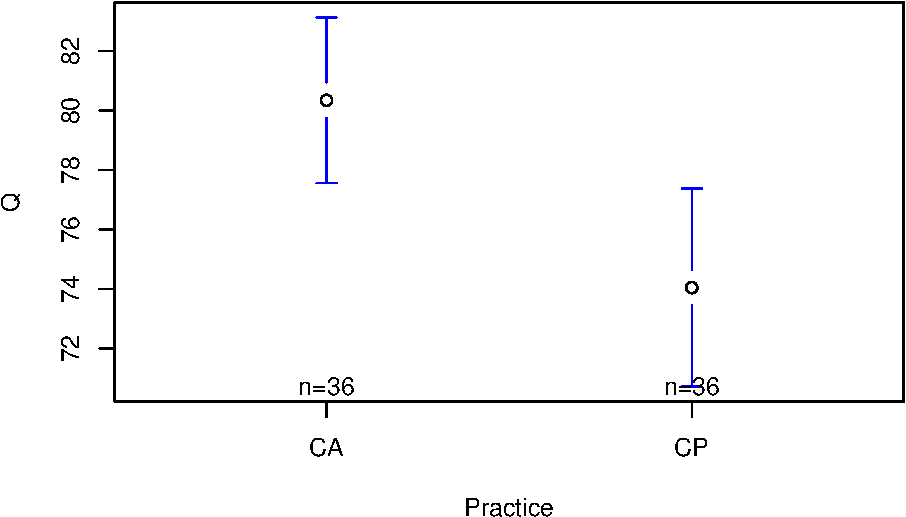
\includegraphics{Doc_pdf_files/figure-latex/unnamed-chunk-12-1.pdf}

\begin{Shaded}
\begin{Highlighting}[]
\FunctionTok{plotmeans}\NormalTok{(Q}\SpecialCharTok{\textasciitilde{}}\NormalTok{Soil, FD\_q0, }\AttributeTok{connect=}\NormalTok{F)}
\end{Highlighting}
\end{Shaded}

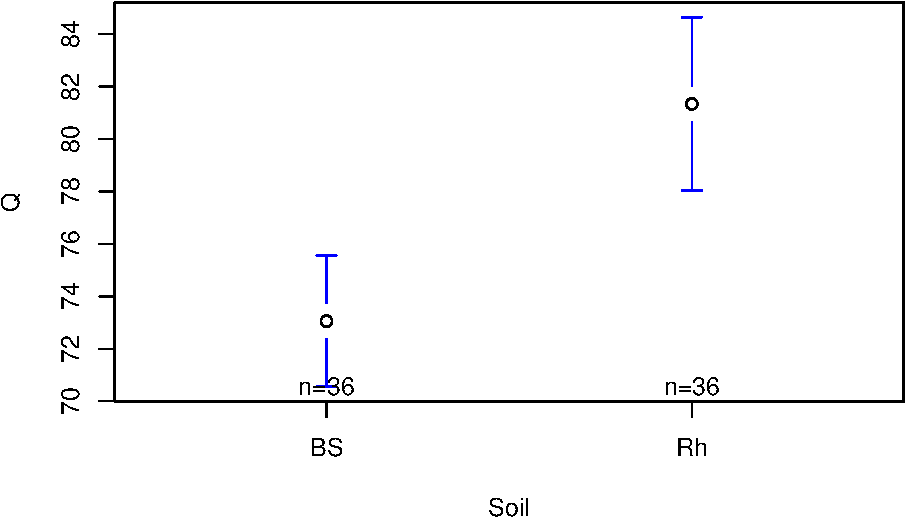
\includegraphics{Doc_pdf_files/figure-latex/unnamed-chunk-12-2.pdf}

\begin{Shaded}
\begin{Highlighting}[]
\FunctionTok{plotmeans}\NormalTok{(Q}\SpecialCharTok{\textasciitilde{}}\NormalTok{Stage, FD\_q1, }\AttributeTok{connect=}\NormalTok{F)}
\end{Highlighting}
\end{Shaded}

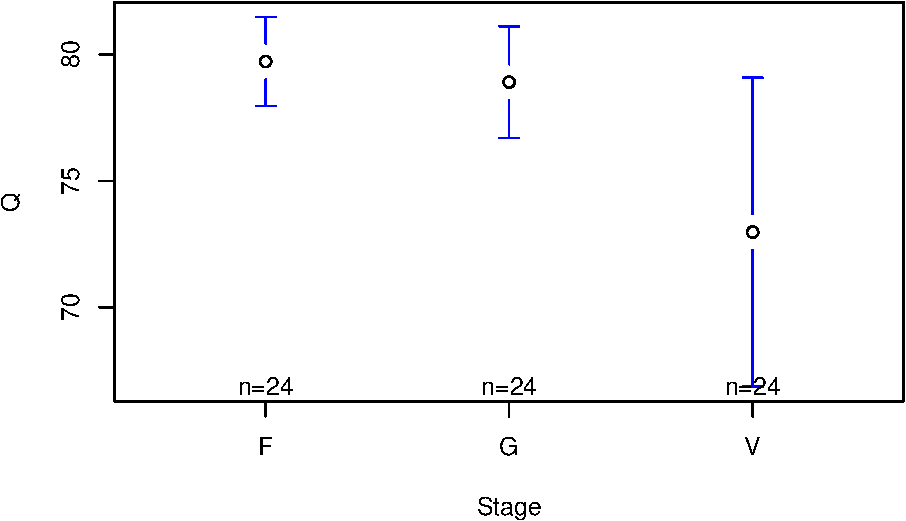
\includegraphics{Doc_pdf_files/figure-latex/unnamed-chunk-12-3.pdf}

\begin{Shaded}
\begin{Highlighting}[]
\FunctionTok{plotmeans}\NormalTok{(Q}\SpecialCharTok{\textasciitilde{}}\NormalTok{Practice, FD\_q0, }\AttributeTok{connect=}\NormalTok{F)}
\end{Highlighting}
\end{Shaded}

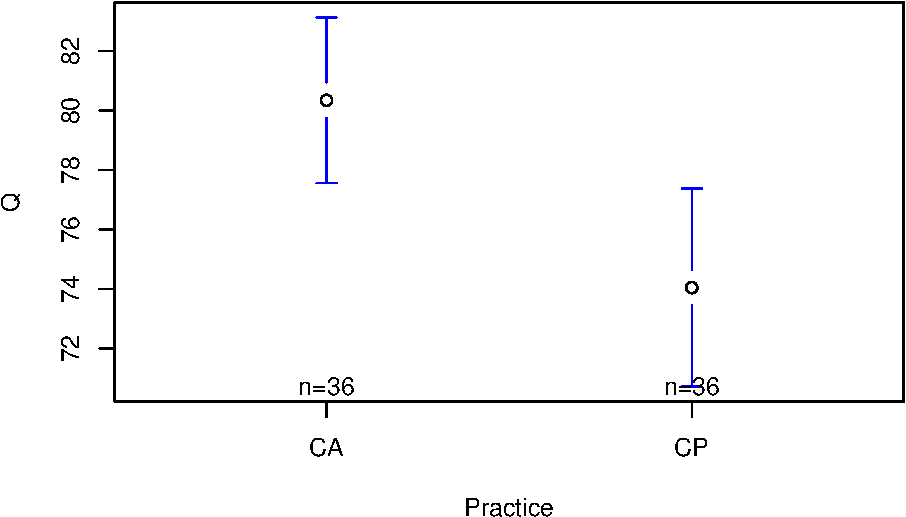
\includegraphics{Doc_pdf_files/figure-latex/unnamed-chunk-12-4.pdf}

\begin{Shaded}
\begin{Highlighting}[]
\FunctionTok{plotmeans}\NormalTok{(FD\_q}\SpecialCharTok{\textasciitilde{}}\NormalTok{Stage, FD\_q1, }\AttributeTok{connect=}\NormalTok{F)}
\end{Highlighting}
\end{Shaded}

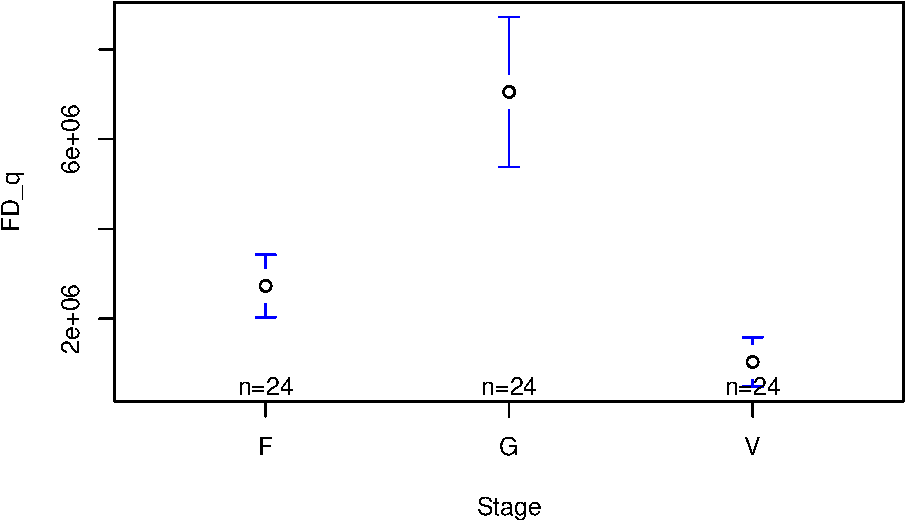
\includegraphics{Doc_pdf_files/figure-latex/unnamed-chunk-12-5.pdf}

\begin{Shaded}
\begin{Highlighting}[]
\FunctionTok{plotmeans}\NormalTok{(D\_q}\SpecialCharTok{\textasciitilde{}}\NormalTok{Soil, FD\_q0, }\AttributeTok{connect=}\NormalTok{F)}
\end{Highlighting}
\end{Shaded}

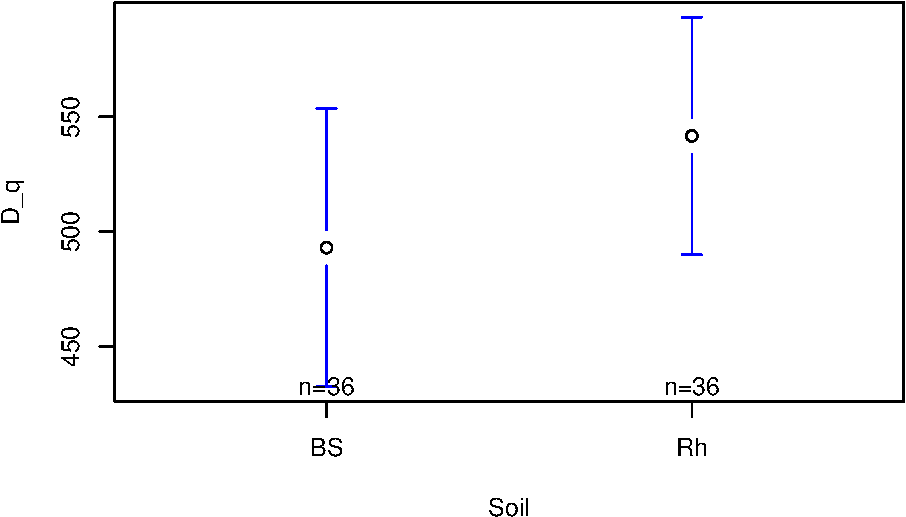
\includegraphics{Doc_pdf_files/figure-latex/unnamed-chunk-12-6.pdf}

\begin{Shaded}
\begin{Highlighting}[]
\FunctionTok{plotmeans}\NormalTok{(D\_q}\SpecialCharTok{\textasciitilde{}}\NormalTok{Soil, FD\_q1, }\AttributeTok{connect=}\NormalTok{F)}
\end{Highlighting}
\end{Shaded}

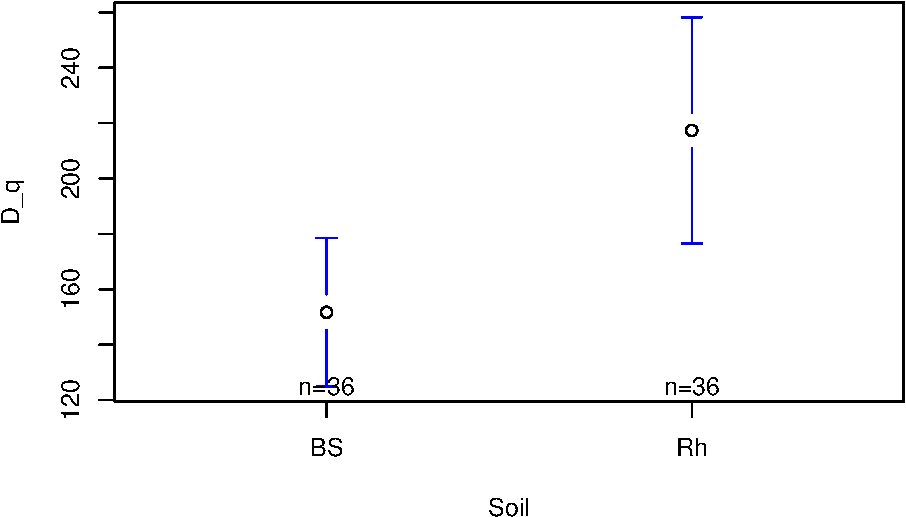
\includegraphics{Doc_pdf_files/figure-latex/unnamed-chunk-12-7.pdf}

\begin{Shaded}
\begin{Highlighting}[]
\FunctionTok{plotmeans}\NormalTok{(D\_q}\SpecialCharTok{\textasciitilde{}}\NormalTok{Soil, FD\_q2, }\AttributeTok{connect=}\NormalTok{F)}
\end{Highlighting}
\end{Shaded}

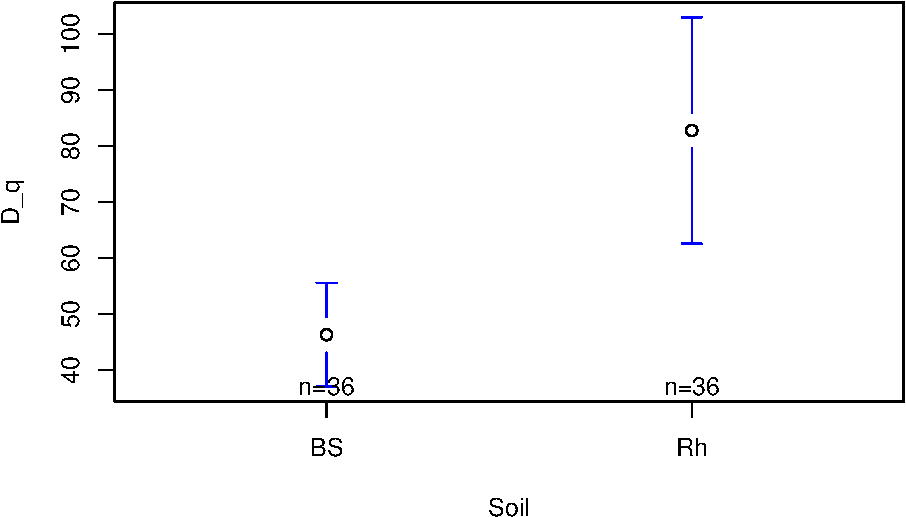
\includegraphics{Doc_pdf_files/figure-latex/unnamed-chunk-12-8.pdf}

\hypertarget{general-linear-model-of-functional-diversity}{%
\subsubsection{General linear model of functional
diversity}\label{general-linear-model-of-functional-diversity}}

\begin{Shaded}
\begin{Highlighting}[]
\NormalTok{func\_MDq}\OtherTok{\textless{}{-}} \FunctionTok{read.delim}\NormalTok{(}\StringTok{"../Data/func\_MDq.txt"}\NormalTok{, }\AttributeTok{check.names =}\NormalTok{ F, }\AttributeTok{row.names =} \DecValTok{1}\NormalTok{)}
  
\NormalTok{a}\OtherTok{\textless{}{-}}\FunctionTok{lme}\NormalTok{(FD\_q}\SpecialCharTok{\textasciitilde{}}\NormalTok{Practice.Location}\SpecialCharTok{*}\NormalTok{Stage, }\AttributeTok{random=}\SpecialCharTok{\textasciitilde{}}\DecValTok{1} \SpecialCharTok{|}\NormalTok{Plot, FD\_q2)}\SpecialCharTok{\%\textgreater{}\%}\NormalTok{PermTest}
\FunctionTok{summary}\NormalTok{(a)}
\end{Highlighting}
\end{Shaded}

\begin{verbatim}
##           Length Class      Mode   
## resultats 1      data.frame list   
## B         1      -none-     numeric
## call      2      -none-     call
\end{verbatim}

\begin{Shaded}
\begin{Highlighting}[]
\NormalTok{b}\OtherTok{\textless{}{-}}\FunctionTok{lme}\NormalTok{(FD\_q}\SpecialCharTok{\textasciitilde{}}\NormalTok{Soil, }\AttributeTok{random=}\SpecialCharTok{\textasciitilde{}}\DecValTok{1} \SpecialCharTok{|}\NormalTok{Plot, FD\_q2)}
\FunctionTok{summary}\NormalTok{(b)}
\end{Highlighting}
\end{Shaded}

\begin{verbatim}
## Linear mixed-effects model fit by REML
##   Data: FD_q2 
##        AIC      BIC    logLik
##   2100.708 2109.702 -1046.354
## 
## Random effects:
##  Formula: ~1 | Plot
##         (Intercept) Residual
## StdDev:    145905.9 704699.1
## 
## Fixed effects:  FD_q ~ Soil 
##                Value Std.Error DF  t-value p-value
## (Intercept) 216353.2  138262.8 67 1.564797  0.1223
## SoilRh      618085.1  166099.2 67 3.721181  0.0004
##  Correlation: 
##        (Intr)
## SoilRh -0.601
## 
## Standardized Within-Group Residuals:
##         Min          Q1         Med          Q3         Max 
## -1.23073653 -0.63084391 -0.15614166  0.08395973  3.69128696 
## 
## Number of Observations: 72
## Number of Groups: 4
\end{verbatim}

\begin{Shaded}
\begin{Highlighting}[]
\NormalTok{c}\OtherTok{\textless{}{-}} \FunctionTok{lme}\NormalTok{(FD\_q}\SpecialCharTok{\textasciitilde{}}\NormalTok{Stage, }\AttributeTok{random=}\SpecialCharTok{\textasciitilde{}}\DecValTok{1} \SpecialCharTok{|}\NormalTok{Plot, FD\_q2)}\SpecialCharTok{\%\textgreater{}\%}
\NormalTok{PermTest}


\NormalTok{O}\OtherTok{\textless{}{-}}\FunctionTok{ggplot}\NormalTok{(func\_MDq, }\FunctionTok{aes}\NormalTok{(}\AttributeTok{x=}\NormalTok{Practice, }\AttributeTok{y=}\NormalTok{MD\_q0, }\AttributeTok{fill=}\NormalTok{Soil))}\SpecialCharTok{+}
  \FunctionTok{geom\_boxplot}\NormalTok{()}
  

\NormalTok{I}\OtherTok{\textless{}{-}}\FunctionTok{ggplot}\NormalTok{(FD\_q1, }\FunctionTok{aes}\NormalTok{(}\AttributeTok{x=}\NormalTok{Practice, }\AttributeTok{y=}\NormalTok{MD\_q, }\AttributeTok{fill=}\NormalTok{Soil))}\SpecialCharTok{+}
  \FunctionTok{geom\_boxplot}\NormalTok{()}

\NormalTok{II}\OtherTok{\textless{}{-}} \FunctionTok{ggplot}\NormalTok{(FD\_q2, }\FunctionTok{aes}\NormalTok{(}\AttributeTok{x=}\NormalTok{Practice, }\AttributeTok{y=}\NormalTok{MD\_q, }\AttributeTok{fill=}\NormalTok{Soil))}\SpecialCharTok{+}
  \FunctionTok{geom\_boxplot}\NormalTok{()}
  
\NormalTok{Os}\OtherTok{\textless{}{-}}\FunctionTok{ggplot}\NormalTok{(FD\_q0, }\FunctionTok{aes}\NormalTok{(}\AttributeTok{x=}\NormalTok{Soil, }\AttributeTok{y=}\NormalTok{MD\_q, }\AttributeTok{fill=}\NormalTok{Stage))}\SpecialCharTok{+}
  \FunctionTok{geom\_boxplot}\NormalTok{()}

\NormalTok{Is}\OtherTok{\textless{}{-}}\FunctionTok{ggplot}\NormalTok{(FD\_q1, }\FunctionTok{aes}\NormalTok{(}\AttributeTok{x=}\NormalTok{Soil, }\AttributeTok{y=}\NormalTok{MD\_q, }\AttributeTok{fill=}\NormalTok{Stage))}\SpecialCharTok{+}
  \FunctionTok{geom\_boxplot}\NormalTok{()}

\NormalTok{IIs}\OtherTok{\textless{}{-}} \FunctionTok{ggplot}\NormalTok{(FD\_q2, }\FunctionTok{aes}\NormalTok{(}\AttributeTok{x=}\NormalTok{Soil, }\AttributeTok{y=}\NormalTok{MD\_q, }\AttributeTok{fill=}\NormalTok{Stage))}\SpecialCharTok{+}
  \FunctionTok{geom\_boxplot}\NormalTok{()}

\NormalTok{Oss}\OtherTok{\textless{}{-}}\FunctionTok{ggplot}\NormalTok{(FD\_q0, }\FunctionTok{aes}\NormalTok{(}\AttributeTok{x=}\NormalTok{Practice.Location, }\AttributeTok{y=}\NormalTok{MD\_q, }\AttributeTok{fill=}\NormalTok{Stage))}\SpecialCharTok{+}
  \FunctionTok{geom\_boxplot}\NormalTok{()}

\NormalTok{Iss}\OtherTok{\textless{}{-}}\FunctionTok{ggplot}\NormalTok{(FD\_q1, }\FunctionTok{aes}\NormalTok{(}\AttributeTok{x=}\NormalTok{Practice.Location, }\AttributeTok{y=}\NormalTok{MD\_q, }\AttributeTok{fill=}\NormalTok{Stage))}\SpecialCharTok{+}
  \FunctionTok{geom\_boxplot}\NormalTok{()}

\NormalTok{IIss}\OtherTok{\textless{}{-}} \FunctionTok{ggplot}\NormalTok{(FD\_q2, }\FunctionTok{aes}\NormalTok{(}\AttributeTok{x=}\NormalTok{Practice.Location, }\AttributeTok{y=}\NormalTok{MD\_q, }\AttributeTok{fill=}\NormalTok{Stage))}\SpecialCharTok{+}
  \FunctionTok{geom\_boxplot}\NormalTok{()}

\NormalTok{r}\OtherTok{\textless{}{-}}\FunctionTok{plot\_grid}\NormalTok{(O, I, II, Os, Is, IIs, Oss, Iss, IIss, }
          \AttributeTok{labels =} \StringTok{"AUTO"}\NormalTok{, }
          \AttributeTok{label\_size =} \DecValTok{17}\NormalTok{, }\AttributeTok{nrow=}\DecValTok{3}\NormalTok{, }\AttributeTok{ncol =} \DecValTok{3}\NormalTok{)}
\NormalTok{r}
\end{Highlighting}
\end{Shaded}

\begin{center}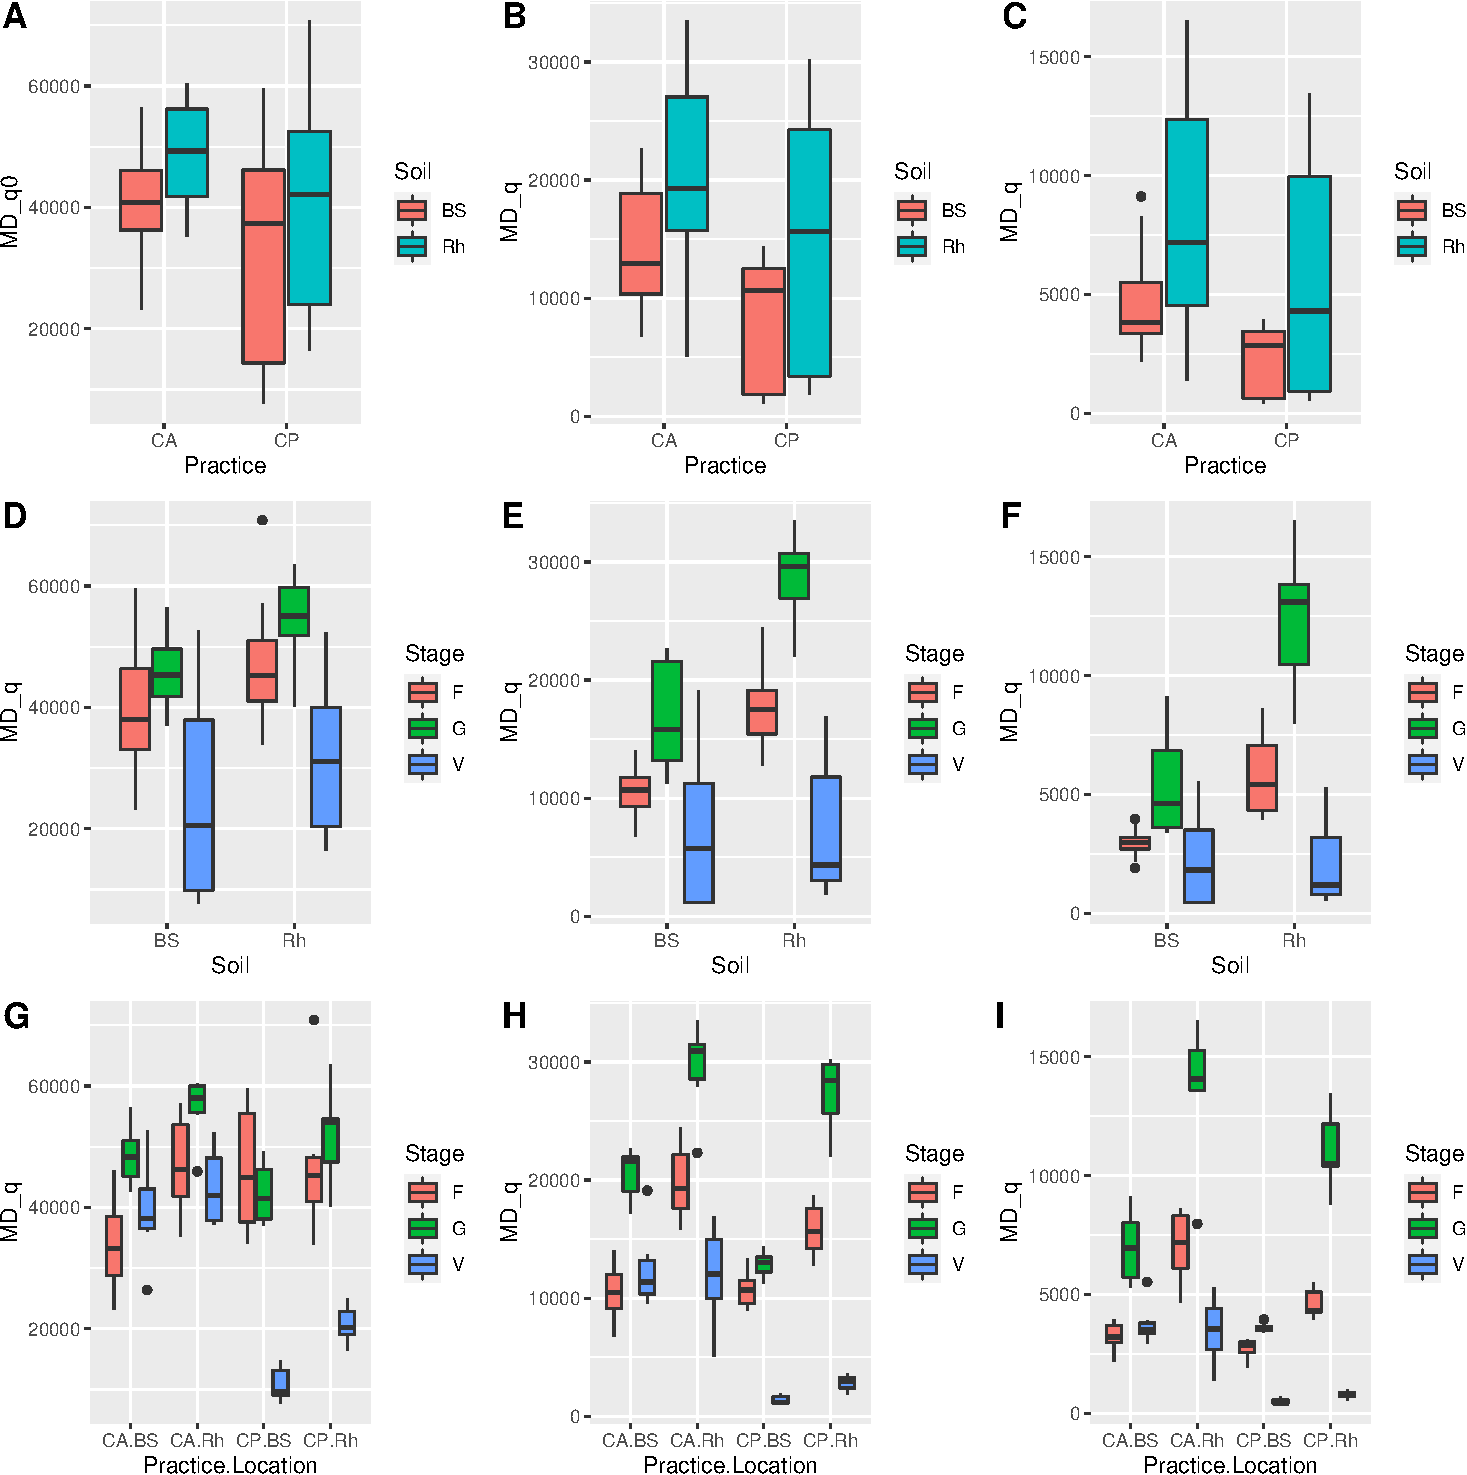
\includegraphics{Doc_pdf_files/figure-latex/unnamed-chunk-13-1} \end{center}

\begin{Shaded}
\begin{Highlighting}[]
\CommentTok{\#pdf("FigX\_FUNDIV{-}interactions.pdf", width=10, height=8)}
\CommentTok{\#print(r)}
\CommentTok{\#dev.off()}
\end{Highlighting}
\end{Shaded}

Plot S3

\begin{Shaded}
\begin{Highlighting}[]
\FunctionTok{library}\NormalTok{(ggpubr)}
\FunctionTok{library}\NormalTok{(cowplot)}
\NormalTok{func\_MDq }\OtherTok{\textless{}{-}} \FunctionTok{read.delim}\NormalTok{(}\StringTok{"../Data/func\_MDq.txt"}\NormalTok{, }\AttributeTok{row.names=}\DecValTok{1}\NormalTok{)}

\NormalTok{F0.p }\OtherTok{\textless{}{-}} \FunctionTok{ggboxplot}\NormalTok{(}\AttributeTok{data =}\NormalTok{ func\_MDq, }\AttributeTok{x =} \StringTok{"Practice"}\NormalTok{, }\AttributeTok{y=} \StringTok{"MD\_q0"}\NormalTok{,}
                \AttributeTok{fill=} \StringTok{"Practice"}\NormalTok{, }\AttributeTok{palette =} \FunctionTok{c}\NormalTok{(}\StringTok{"\#212F3D"}\NormalTok{, }\StringTok{"\#839192"}\NormalTok{), }
                \AttributeTok{width =} \FloatTok{0.6}\NormalTok{, }\AttributeTok{lwd=}\FloatTok{0.8}\NormalTok{, }\AttributeTok{facet.by =} \StringTok{"Stage"}\NormalTok{)  }\SpecialCharTok{+}
    \FunctionTok{labs}\NormalTok{(}\AttributeTok{x =} \FunctionTok{element\_blank}\NormalTok{(), }\AttributeTok{y =} \StringTok{"Mean functional diversity"}\NormalTok{)}\SpecialCharTok{+}
  \FunctionTok{theme\_gray}\NormalTok{() }\SpecialCharTok{+}
  \FunctionTok{theme}\NormalTok{(}\AttributeTok{text =} \FunctionTok{element\_text}\NormalTok{ (}\AttributeTok{size =} \DecValTok{12}\NormalTok{))}\SpecialCharTok{+}
  \FunctionTok{theme}\NormalTok{(}\AttributeTok{legend.position =} \StringTok{"none"}\NormalTok{)}\SpecialCharTok{+}
  \FunctionTok{theme}\NormalTok{(}\AttributeTok{plot.title =} \FunctionTok{element\_text}\NormalTok{(}\StringTok{"q=0"}\NormalTok{))}\SpecialCharTok{+}
  \FunctionTok{theme}\NormalTok{(}\AttributeTok{legend.position =} \StringTok{"none"}\NormalTok{,}
        \AttributeTok{axis.ticks.x =} \FunctionTok{element\_blank}\NormalTok{())}\SpecialCharTok{+}
  \FunctionTok{stat\_compare\_means}\NormalTok{(}\AttributeTok{method =} \StringTok{"t.test"}\NormalTok{)}
\NormalTok{F1.p }\OtherTok{\textless{}{-}} \FunctionTok{ggboxplot}\NormalTok{(}\AttributeTok{data =}\NormalTok{ func\_MDq, }\AttributeTok{x =} \StringTok{"Practice"}\NormalTok{, }\AttributeTok{y=} \StringTok{"MD\_q1"}\NormalTok{,}
                  \AttributeTok{fill =} \StringTok{"Practice"}\NormalTok{, }\AttributeTok{palette =} \FunctionTok{c}\NormalTok{(}\StringTok{"\#212F3D"}\NormalTok{, }\StringTok{"\#839192"}\NormalTok{), }
                  \AttributeTok{width =} \FloatTok{0.6}\NormalTok{, }\AttributeTok{lwd=}\FloatTok{0.8}\NormalTok{, }\AttributeTok{facet.by =} \StringTok{"Stage"}\NormalTok{)  }\SpecialCharTok{+}
  \FunctionTok{labs}\NormalTok{(}\AttributeTok{x =} \FunctionTok{element\_blank}\NormalTok{(), }\AttributeTok{y =} \StringTok{"Mean functional diversity"}\NormalTok{)}\SpecialCharTok{+}
  \FunctionTok{theme\_gray}\NormalTok{() }\SpecialCharTok{+}
  \FunctionTok{theme}\NormalTok{(}\AttributeTok{text =} \FunctionTok{element\_text}\NormalTok{ (}\AttributeTok{size =} \DecValTok{12}\NormalTok{))}\SpecialCharTok{+}
  \FunctionTok{theme}\NormalTok{(}\AttributeTok{legend.position =} \StringTok{"none"}\NormalTok{)}\SpecialCharTok{+}
  \FunctionTok{theme}\NormalTok{(}\AttributeTok{plot.title =} \FunctionTok{element\_text}\NormalTok{(}\StringTok{"q=0"}\NormalTok{))}\SpecialCharTok{+}
  \FunctionTok{theme}\NormalTok{(}\AttributeTok{legend.position =} \StringTok{"none"}\NormalTok{,}
        \AttributeTok{axis.ticks.x =} \FunctionTok{element\_blank}\NormalTok{())}\SpecialCharTok{+}
  \FunctionTok{stat\_compare\_means}\NormalTok{(}\AttributeTok{method =} \StringTok{"t.test"}\NormalTok{)}
\NormalTok{F2.p }\OtherTok{\textless{}{-}} \FunctionTok{ggboxplot}\NormalTok{(}\AttributeTok{data =}\NormalTok{ func\_MDq, }\AttributeTok{x =} \StringTok{"Practice"}\NormalTok{, }\AttributeTok{y=} \StringTok{"MD\_q2"}\NormalTok{,}
                  \AttributeTok{fill =} \StringTok{"Practice"}\NormalTok{, }\AttributeTok{palette =} \FunctionTok{c}\NormalTok{(}\StringTok{"\#212F3D"}\NormalTok{, }\StringTok{"\#839192"}\NormalTok{), }
                  \AttributeTok{width =} \FloatTok{0.6}\NormalTok{, }\AttributeTok{lwd=}\FloatTok{0.8}\NormalTok{, }\AttributeTok{facet.by =} \StringTok{"Stage"}\NormalTok{)  }\SpecialCharTok{+}
  \FunctionTok{labs}\NormalTok{(}\AttributeTok{x =} \FunctionTok{element\_blank}\NormalTok{(), }\AttributeTok{y =} \StringTok{"Mean functional diversity"}\NormalTok{)}\SpecialCharTok{+}
  \FunctionTok{theme\_gray}\NormalTok{() }\SpecialCharTok{+}
  \FunctionTok{theme}\NormalTok{(}\AttributeTok{text =} \FunctionTok{element\_text}\NormalTok{ (}\AttributeTok{size =} \DecValTok{12}\NormalTok{))}\SpecialCharTok{+}
  \FunctionTok{theme}\NormalTok{(}\AttributeTok{legend.position =} \StringTok{"none"}\NormalTok{)}\SpecialCharTok{+}
  \FunctionTok{theme}\NormalTok{(}\AttributeTok{plot.title =} \FunctionTok{element\_text}\NormalTok{(}\StringTok{"q=0"}\NormalTok{))}\SpecialCharTok{+}
  \FunctionTok{theme}\NormalTok{(}\AttributeTok{legend.position =} \StringTok{"none"}\NormalTok{,}
        \AttributeTok{axis.ticks.x =} \FunctionTok{element\_blank}\NormalTok{())}\SpecialCharTok{+}
  \FunctionTok{stat\_compare\_means}\NormalTok{(}\AttributeTok{method =} \StringTok{"t.test"}\NormalTok{)}
        
\NormalTok{F0.s }\OtherTok{\textless{}{-}} \FunctionTok{ggboxplot}\NormalTok{(}\AttributeTok{data =}\NormalTok{ func\_MDq, }\AttributeTok{x =} \StringTok{"Soil"}\NormalTok{, }\AttributeTok{y=} \StringTok{"MD\_q0"}\NormalTok{,}
                  \AttributeTok{fill =} \StringTok{"Soil"}\NormalTok{, }\AttributeTok{palette =} \FunctionTok{c}\NormalTok{(}\StringTok{"darkgoldenrod4"}\NormalTok{, }\StringTok{"\#365238"}\NormalTok{), }
                  \AttributeTok{width =} \FloatTok{0.6}\NormalTok{, }\AttributeTok{lwd=}\FloatTok{0.8}\NormalTok{, }\AttributeTok{facet.by =} \StringTok{"Stage"}\NormalTok{)  }\SpecialCharTok{+}
  \FunctionTok{labs}\NormalTok{(}\AttributeTok{x =} \FunctionTok{element\_blank}\NormalTok{(), }\AttributeTok{y =} \StringTok{"Mean functional diversity"}\NormalTok{)}\SpecialCharTok{+}
  \FunctionTok{theme\_gray}\NormalTok{() }\SpecialCharTok{+}
  \FunctionTok{theme}\NormalTok{(}\AttributeTok{text =} \FunctionTok{element\_text}\NormalTok{ (}\AttributeTok{size =} \DecValTok{12}\NormalTok{))}\SpecialCharTok{+}
  \FunctionTok{theme}\NormalTok{(}\AttributeTok{legend.position =} \StringTok{"none"}\NormalTok{)}\SpecialCharTok{+}
  \FunctionTok{theme}\NormalTok{(}\AttributeTok{plot.title =} \FunctionTok{element\_text}\NormalTok{(}\StringTok{"q=0"}\NormalTok{))}\SpecialCharTok{+}
  \FunctionTok{theme}\NormalTok{(}\AttributeTok{legend.position =} \StringTok{"none"}\NormalTok{,}
        \AttributeTok{axis.ticks.x =} \FunctionTok{element\_blank}\NormalTok{())}\SpecialCharTok{+}
  \FunctionTok{stat\_compare\_means}\NormalTok{(}\AttributeTok{method =} \StringTok{"t.test"}\NormalTok{)}
\NormalTok{F1.s }\OtherTok{\textless{}{-}} \FunctionTok{ggboxplot}\NormalTok{(}\AttributeTok{data =}\NormalTok{ func\_MDq, }\AttributeTok{x =} \StringTok{"Soil"}\NormalTok{, }\AttributeTok{y=} \StringTok{"MD\_q1"}\NormalTok{,}
                  \AttributeTok{fill =} \StringTok{"Soil"}\NormalTok{, }\AttributeTok{palette =} \FunctionTok{c}\NormalTok{(}\StringTok{"darkgoldenrod4"}\NormalTok{, }\StringTok{"\#365238"}\NormalTok{), }
                  \AttributeTok{width =} \FloatTok{0.6}\NormalTok{, }\AttributeTok{lwd=}\FloatTok{0.8}\NormalTok{, }\AttributeTok{facet.by =} \StringTok{"Stage"}\NormalTok{)  }\SpecialCharTok{+}
  \FunctionTok{labs}\NormalTok{(}\AttributeTok{x =} \FunctionTok{element\_blank}\NormalTok{(), }\AttributeTok{y =} \StringTok{"Mean functional diversity"}\NormalTok{)}\SpecialCharTok{+}
  \FunctionTok{theme\_gray}\NormalTok{() }\SpecialCharTok{+}
  \FunctionTok{theme}\NormalTok{(}\AttributeTok{text =} \FunctionTok{element\_text}\NormalTok{ (}\AttributeTok{size =} \DecValTok{12}\NormalTok{))}\SpecialCharTok{+}
  \FunctionTok{theme}\NormalTok{(}\AttributeTok{legend.position =} \StringTok{"none"}\NormalTok{)}\SpecialCharTok{+}
  \FunctionTok{theme}\NormalTok{(}\AttributeTok{plot.title =} \FunctionTok{element\_text}\NormalTok{(}\StringTok{"q=0"}\NormalTok{))}\SpecialCharTok{+}
  \FunctionTok{theme}\NormalTok{(}\AttributeTok{legend.position =} \StringTok{"none"}\NormalTok{,}
        \AttributeTok{axis.ticks.x =} \FunctionTok{element\_blank}\NormalTok{())}\SpecialCharTok{+}
  \FunctionTok{stat\_compare\_means}\NormalTok{(}\AttributeTok{method =} \StringTok{"t.test"}\NormalTok{)}
\NormalTok{F2.s }\OtherTok{\textless{}{-}} \FunctionTok{ggboxplot}\NormalTok{(}\AttributeTok{data =}\NormalTok{ func\_MDq, }\AttributeTok{x =} \StringTok{"Soil"}\NormalTok{, }\AttributeTok{y=} \StringTok{"MD\_q2"}\NormalTok{,}
                  \AttributeTok{fill =} \StringTok{"Soil"}\NormalTok{, }\AttributeTok{palette =} \FunctionTok{c}\NormalTok{(}\StringTok{"darkgoldenrod4"}\NormalTok{, }\StringTok{"\#365238"}\NormalTok{), }
                  \AttributeTok{width =} \FloatTok{0.6}\NormalTok{, }\AttributeTok{lwd=}\FloatTok{0.8}\NormalTok{, }\AttributeTok{facet.by =} \StringTok{"Stage"}\NormalTok{)  }\SpecialCharTok{+}
  \FunctionTok{labs}\NormalTok{(}\AttributeTok{x =} \FunctionTok{element\_blank}\NormalTok{(), }\AttributeTok{y =} \StringTok{"Mean functional diversity"}\NormalTok{)}\SpecialCharTok{+}
  \FunctionTok{theme\_gray}\NormalTok{() }\SpecialCharTok{+}
  \FunctionTok{theme}\NormalTok{(}\AttributeTok{text =} \FunctionTok{element\_text}\NormalTok{ (}\AttributeTok{size =} \DecValTok{12}\NormalTok{))}\SpecialCharTok{+}
  \FunctionTok{theme}\NormalTok{(}\AttributeTok{legend.position =} \StringTok{"none"}\NormalTok{)}\SpecialCharTok{+}
  \FunctionTok{theme}\NormalTok{(}\AttributeTok{plot.title =} \FunctionTok{element\_text}\NormalTok{(}\StringTok{"q=0"}\NormalTok{))}\SpecialCharTok{+}
  \FunctionTok{theme}\NormalTok{(}\AttributeTok{legend.position =} \StringTok{"none"}\NormalTok{,}
        \AttributeTok{axis.ticks.x =} \FunctionTok{element\_blank}\NormalTok{())}\SpecialCharTok{+}
  \FunctionTok{stat\_compare\_means}\NormalTok{(}\AttributeTok{method =} \StringTok{"t.test"}\NormalTok{)}

\NormalTok{div }\OtherTok{\textless{}{-}} \FunctionTok{read.delim}\NormalTok{(}\StringTok{"../Data/Alpha{-}t\_asv\_table.txt"}\NormalTok{, }\AttributeTok{row.names=}\DecValTok{1}\NormalTok{)}

\NormalTok{D0.p }\OtherTok{\textless{}{-}} \FunctionTok{ggboxplot}\NormalTok{(}\AttributeTok{data =}\NormalTok{ div, }\AttributeTok{x =} \StringTok{"Practice"}\NormalTok{, }\AttributeTok{y=} \StringTok{"q0"}\NormalTok{,}
                  \AttributeTok{fill =} \StringTok{"Practice"}\NormalTok{, }\AttributeTok{palette =} \FunctionTok{c}\NormalTok{(}\StringTok{"\#212F3D"}\NormalTok{, }\StringTok{"\#839192"}\NormalTok{), }
                  \AttributeTok{width =} \FloatTok{0.6}\NormalTok{, }\AttributeTok{lwd=}\FloatTok{0.8}\NormalTok{, }\AttributeTok{facet.by =} \StringTok{"Stage"}\NormalTok{)  }\SpecialCharTok{+}
  \FunctionTok{labs}\NormalTok{(}\AttributeTok{x =} \FunctionTok{element\_blank}\NormalTok{(), }\AttributeTok{y =} \StringTok{"Effective number of OTUs"}\NormalTok{)}\SpecialCharTok{+}
  \FunctionTok{theme\_gray}\NormalTok{() }\SpecialCharTok{+}
  \FunctionTok{theme}\NormalTok{(}\AttributeTok{text =} \FunctionTok{element\_text}\NormalTok{ (}\AttributeTok{size =} \DecValTok{12}\NormalTok{))}\SpecialCharTok{+}
  \FunctionTok{theme}\NormalTok{(}\AttributeTok{legend.position =} \StringTok{"none"}\NormalTok{)}\SpecialCharTok{+}
  \FunctionTok{theme}\NormalTok{(}\AttributeTok{plot.title =} \FunctionTok{element\_text}\NormalTok{(}\StringTok{"q=0"}\NormalTok{))}\SpecialCharTok{+}
  \FunctionTok{theme}\NormalTok{(}\AttributeTok{legend.position =} \StringTok{"none"}\NormalTok{,}
        \AttributeTok{axis.ticks.x =} \FunctionTok{element\_blank}\NormalTok{())}\SpecialCharTok{+}
  \FunctionTok{stat\_compare\_means}\NormalTok{(}\AttributeTok{method =} \StringTok{"t.test"}\NormalTok{)}
\NormalTok{D1.p }\OtherTok{\textless{}{-}} \FunctionTok{ggboxplot}\NormalTok{(}\AttributeTok{data =}\NormalTok{ div, }\AttributeTok{x =} \StringTok{"Practice"}\NormalTok{, }\AttributeTok{y=} \StringTok{"q1"}\NormalTok{,}
                  \AttributeTok{fill =} \StringTok{"Practice"}\NormalTok{, }\AttributeTok{palette =} \FunctionTok{c}\NormalTok{(}\StringTok{"\#212F3D"}\NormalTok{, }\StringTok{"\#839192"}\NormalTok{), }
                  \AttributeTok{width =} \FloatTok{0.6}\NormalTok{, }\AttributeTok{lwd=}\FloatTok{0.8}\NormalTok{, }\AttributeTok{facet.by =} \StringTok{"Stage"}\NormalTok{)  }\SpecialCharTok{+}
  \FunctionTok{labs}\NormalTok{(}\AttributeTok{x =} \FunctionTok{element\_blank}\NormalTok{(), }\AttributeTok{y =} \StringTok{"Effective number of OTUs"}\NormalTok{)}\SpecialCharTok{+}
  \FunctionTok{theme\_gray}\NormalTok{() }\SpecialCharTok{+}
  \FunctionTok{theme}\NormalTok{(}\AttributeTok{text =} \FunctionTok{element\_text}\NormalTok{ (}\AttributeTok{size =} \DecValTok{12}\NormalTok{))}\SpecialCharTok{+}
  \FunctionTok{theme}\NormalTok{(}\AttributeTok{legend.position =} \StringTok{"none"}\NormalTok{)}\SpecialCharTok{+}
  \FunctionTok{theme}\NormalTok{(}\AttributeTok{plot.title =} \FunctionTok{element\_text}\NormalTok{(}\StringTok{"q=0"}\NormalTok{))}\SpecialCharTok{+}
  \FunctionTok{theme}\NormalTok{(}\AttributeTok{legend.position =} \StringTok{"none"}\NormalTok{,}
        \AttributeTok{axis.ticks.x =} \FunctionTok{element\_blank}\NormalTok{())}\SpecialCharTok{+}
  \FunctionTok{stat\_compare\_means}\NormalTok{(}\AttributeTok{method =} \StringTok{"t.test"}\NormalTok{)}

\NormalTok{D2.p }\OtherTok{\textless{}{-}} \FunctionTok{ggboxplot}\NormalTok{(}\AttributeTok{data =}\NormalTok{ div, }\AttributeTok{x =} \StringTok{"Practice"}\NormalTok{, }\AttributeTok{y=} \StringTok{"q2"}\NormalTok{,}
                  \AttributeTok{fill =} \StringTok{"Practice"}\NormalTok{, }\AttributeTok{palette =} \FunctionTok{c}\NormalTok{(}\StringTok{"\#212F3D"}\NormalTok{, }\StringTok{"\#839192"}\NormalTok{), }
                  \AttributeTok{width =} \FloatTok{0.6}\NormalTok{, }\AttributeTok{lwd=}\FloatTok{0.8}\NormalTok{, }\AttributeTok{facet.by =} \StringTok{"Stage"}\NormalTok{)  }\SpecialCharTok{+}
  \FunctionTok{labs}\NormalTok{(}\AttributeTok{x =} \FunctionTok{element\_blank}\NormalTok{(), }\AttributeTok{y =} \StringTok{"Effective number of OTUs"}\NormalTok{)}\SpecialCharTok{+}
  \FunctionTok{theme\_gray}\NormalTok{() }\SpecialCharTok{+}
  \FunctionTok{theme}\NormalTok{(}\AttributeTok{text =} \FunctionTok{element\_text}\NormalTok{ (}\AttributeTok{size =} \DecValTok{12}\NormalTok{))}\SpecialCharTok{+}
  \FunctionTok{theme}\NormalTok{(}\AttributeTok{legend.position =} \StringTok{"none"}\NormalTok{)}\SpecialCharTok{+}
  \FunctionTok{theme}\NormalTok{(}\AttributeTok{plot.title =} \FunctionTok{element\_text}\NormalTok{(}\StringTok{"q=0"}\NormalTok{))}\SpecialCharTok{+}
  \FunctionTok{theme}\NormalTok{(}\AttributeTok{legend.position =} \StringTok{"none"}\NormalTok{,}
        \AttributeTok{axis.ticks.x =} \FunctionTok{element\_blank}\NormalTok{())}\SpecialCharTok{+}
  \FunctionTok{stat\_compare\_means}\NormalTok{(}\AttributeTok{method =} \StringTok{"t.test"}\NormalTok{)}

\NormalTok{D0.s }\OtherTok{\textless{}{-}} \FunctionTok{ggboxplot}\NormalTok{(}\AttributeTok{data =}\NormalTok{ div, }\AttributeTok{x =} \StringTok{"Soil"}\NormalTok{, }\AttributeTok{y=} \StringTok{"q0"}\NormalTok{,}
                  \AttributeTok{fill =} \StringTok{"Soil"}\NormalTok{, }\AttributeTok{palette =} \FunctionTok{c}\NormalTok{(}\StringTok{"darkgoldenrod4"}\NormalTok{, }\StringTok{"\#365238"}\NormalTok{), }
                  \AttributeTok{width =} \FloatTok{0.6}\NormalTok{, }\AttributeTok{lwd=}\FloatTok{0.8}\NormalTok{, }\AttributeTok{facet.by =} \StringTok{"Stage"}\NormalTok{)  }\SpecialCharTok{+}
  \FunctionTok{labs}\NormalTok{(}\AttributeTok{x =} \FunctionTok{element\_blank}\NormalTok{(), }\AttributeTok{y =} \StringTok{"Effective number of OTUs"}\NormalTok{)}\SpecialCharTok{+}
  \FunctionTok{theme\_gray}\NormalTok{() }\SpecialCharTok{+}
  \FunctionTok{theme}\NormalTok{(}\AttributeTok{text =} \FunctionTok{element\_text}\NormalTok{ (}\AttributeTok{size =} \DecValTok{12}\NormalTok{))}\SpecialCharTok{+}
  \FunctionTok{theme}\NormalTok{(}\AttributeTok{legend.position =} \StringTok{"none"}\NormalTok{)}\SpecialCharTok{+}
  \FunctionTok{theme}\NormalTok{(}\AttributeTok{plot.title =} \FunctionTok{element\_text}\NormalTok{(}\StringTok{"q=0"}\NormalTok{))}\SpecialCharTok{+}
  \FunctionTok{theme}\NormalTok{(}\AttributeTok{legend.position =} \StringTok{"none"}\NormalTok{,}
        \AttributeTok{axis.ticks.x =} \FunctionTok{element\_blank}\NormalTok{())}\SpecialCharTok{+}
  \FunctionTok{stat\_compare\_means}\NormalTok{(}\AttributeTok{method =} \StringTok{"t.test"}\NormalTok{)}
\NormalTok{D1.s }\OtherTok{\textless{}{-}} \FunctionTok{ggboxplot}\NormalTok{(}\AttributeTok{data =}\NormalTok{ div, }\AttributeTok{x =} \StringTok{"Soil"}\NormalTok{, }\AttributeTok{y=} \StringTok{"q1"}\NormalTok{,}
                  \AttributeTok{fill =} \StringTok{"Soil"}\NormalTok{, }\AttributeTok{palette =} \FunctionTok{c}\NormalTok{(}\StringTok{"darkgoldenrod4"}\NormalTok{, }\StringTok{"\#365238"}\NormalTok{), }
                  \AttributeTok{width =} \FloatTok{0.6}\NormalTok{, }\AttributeTok{lwd=}\FloatTok{0.8}\NormalTok{, }\AttributeTok{facet.by =} \StringTok{"Stage"}\NormalTok{)  }\SpecialCharTok{+}
  \FunctionTok{labs}\NormalTok{(}\AttributeTok{x =} \FunctionTok{element\_blank}\NormalTok{(), }\AttributeTok{y =} \StringTok{"Effective number of OTUs"}\NormalTok{)}\SpecialCharTok{+}
  \FunctionTok{theme\_gray}\NormalTok{() }\SpecialCharTok{+}
  \FunctionTok{theme}\NormalTok{(}\AttributeTok{text =} \FunctionTok{element\_text}\NormalTok{ (}\AttributeTok{size =} \DecValTok{12}\NormalTok{))}\SpecialCharTok{+}
  \FunctionTok{theme}\NormalTok{(}\AttributeTok{legend.position =} \StringTok{"none"}\NormalTok{)}\SpecialCharTok{+}
  \FunctionTok{theme}\NormalTok{(}\AttributeTok{plot.title =} \FunctionTok{element\_text}\NormalTok{(}\StringTok{"q=0"}\NormalTok{))}\SpecialCharTok{+}
  \FunctionTok{theme}\NormalTok{(}\AttributeTok{legend.position =} \StringTok{"none"}\NormalTok{,}
        \AttributeTok{axis.ticks.x =} \FunctionTok{element\_blank}\NormalTok{())}\SpecialCharTok{+}
  \FunctionTok{stat\_compare\_means}\NormalTok{(}\AttributeTok{method =} \StringTok{"t.test"}\NormalTok{)}

\NormalTok{D2.s }\OtherTok{\textless{}{-}} \FunctionTok{ggboxplot}\NormalTok{(}\AttributeTok{data =}\NormalTok{ div, }\AttributeTok{x =} \StringTok{"Soil"}\NormalTok{, }\AttributeTok{y=} \StringTok{"q2"}\NormalTok{,}
                  \AttributeTok{fill =} \StringTok{"Soil"}\NormalTok{, }\AttributeTok{palette =} \FunctionTok{c}\NormalTok{(}\StringTok{"darkgoldenrod4"}\NormalTok{, }\StringTok{"\#365238"}\NormalTok{), }
                  \AttributeTok{width =} \FloatTok{0.6}\NormalTok{, }\AttributeTok{lwd=}\FloatTok{0.8}\NormalTok{, }\AttributeTok{facet.by =} \StringTok{"Stage"}\NormalTok{)  }\SpecialCharTok{+}
  \FunctionTok{labs}\NormalTok{(}\AttributeTok{x =} \FunctionTok{element\_blank}\NormalTok{(), }\AttributeTok{y =} \StringTok{"Effective number of OTUs"}\NormalTok{)}\SpecialCharTok{+}
  \FunctionTok{theme\_gray}\NormalTok{() }\SpecialCharTok{+}
  \FunctionTok{theme}\NormalTok{(}\AttributeTok{text =} \FunctionTok{element\_text}\NormalTok{ (}\AttributeTok{size =} \DecValTok{12}\NormalTok{))}\SpecialCharTok{+}
  \FunctionTok{theme}\NormalTok{(}\AttributeTok{legend.position =} \StringTok{"none"}\NormalTok{)}\SpecialCharTok{+}
  \FunctionTok{theme}\NormalTok{(}\AttributeTok{plot.title =} \FunctionTok{element\_text}\NormalTok{(}\StringTok{"q=0"}\NormalTok{))}\SpecialCharTok{+}
  \FunctionTok{theme}\NormalTok{(}\AttributeTok{legend.position =} \StringTok{"none"}\NormalTok{,}
        \AttributeTok{axis.ticks.x =} \FunctionTok{element\_blank}\NormalTok{())}\SpecialCharTok{+}
  \FunctionTok{stat\_compare\_means}\NormalTok{(}\AttributeTok{method =} \StringTok{"t.test"}\NormalTok{)}


\NormalTok{r}\OtherTok{\textless{}{-}}\FunctionTok{plot\_grid}\NormalTok{(D0.p, D1.p,D2.p,D0.s,D1.s,D2.s, F0.p, F1.p,F2.p,F0.s,F1.s,F2.s, }
             \AttributeTok{labels =} \StringTok{"AUTO"}\NormalTok{, }
             \AttributeTok{label\_size =} \DecValTok{17}\NormalTok{, }\AttributeTok{nrow=}\DecValTok{4}\NormalTok{, }\AttributeTok{ncol =} \DecValTok{3}\NormalTok{)}
\NormalTok{r}
\end{Highlighting}
\end{Shaded}

\begin{center}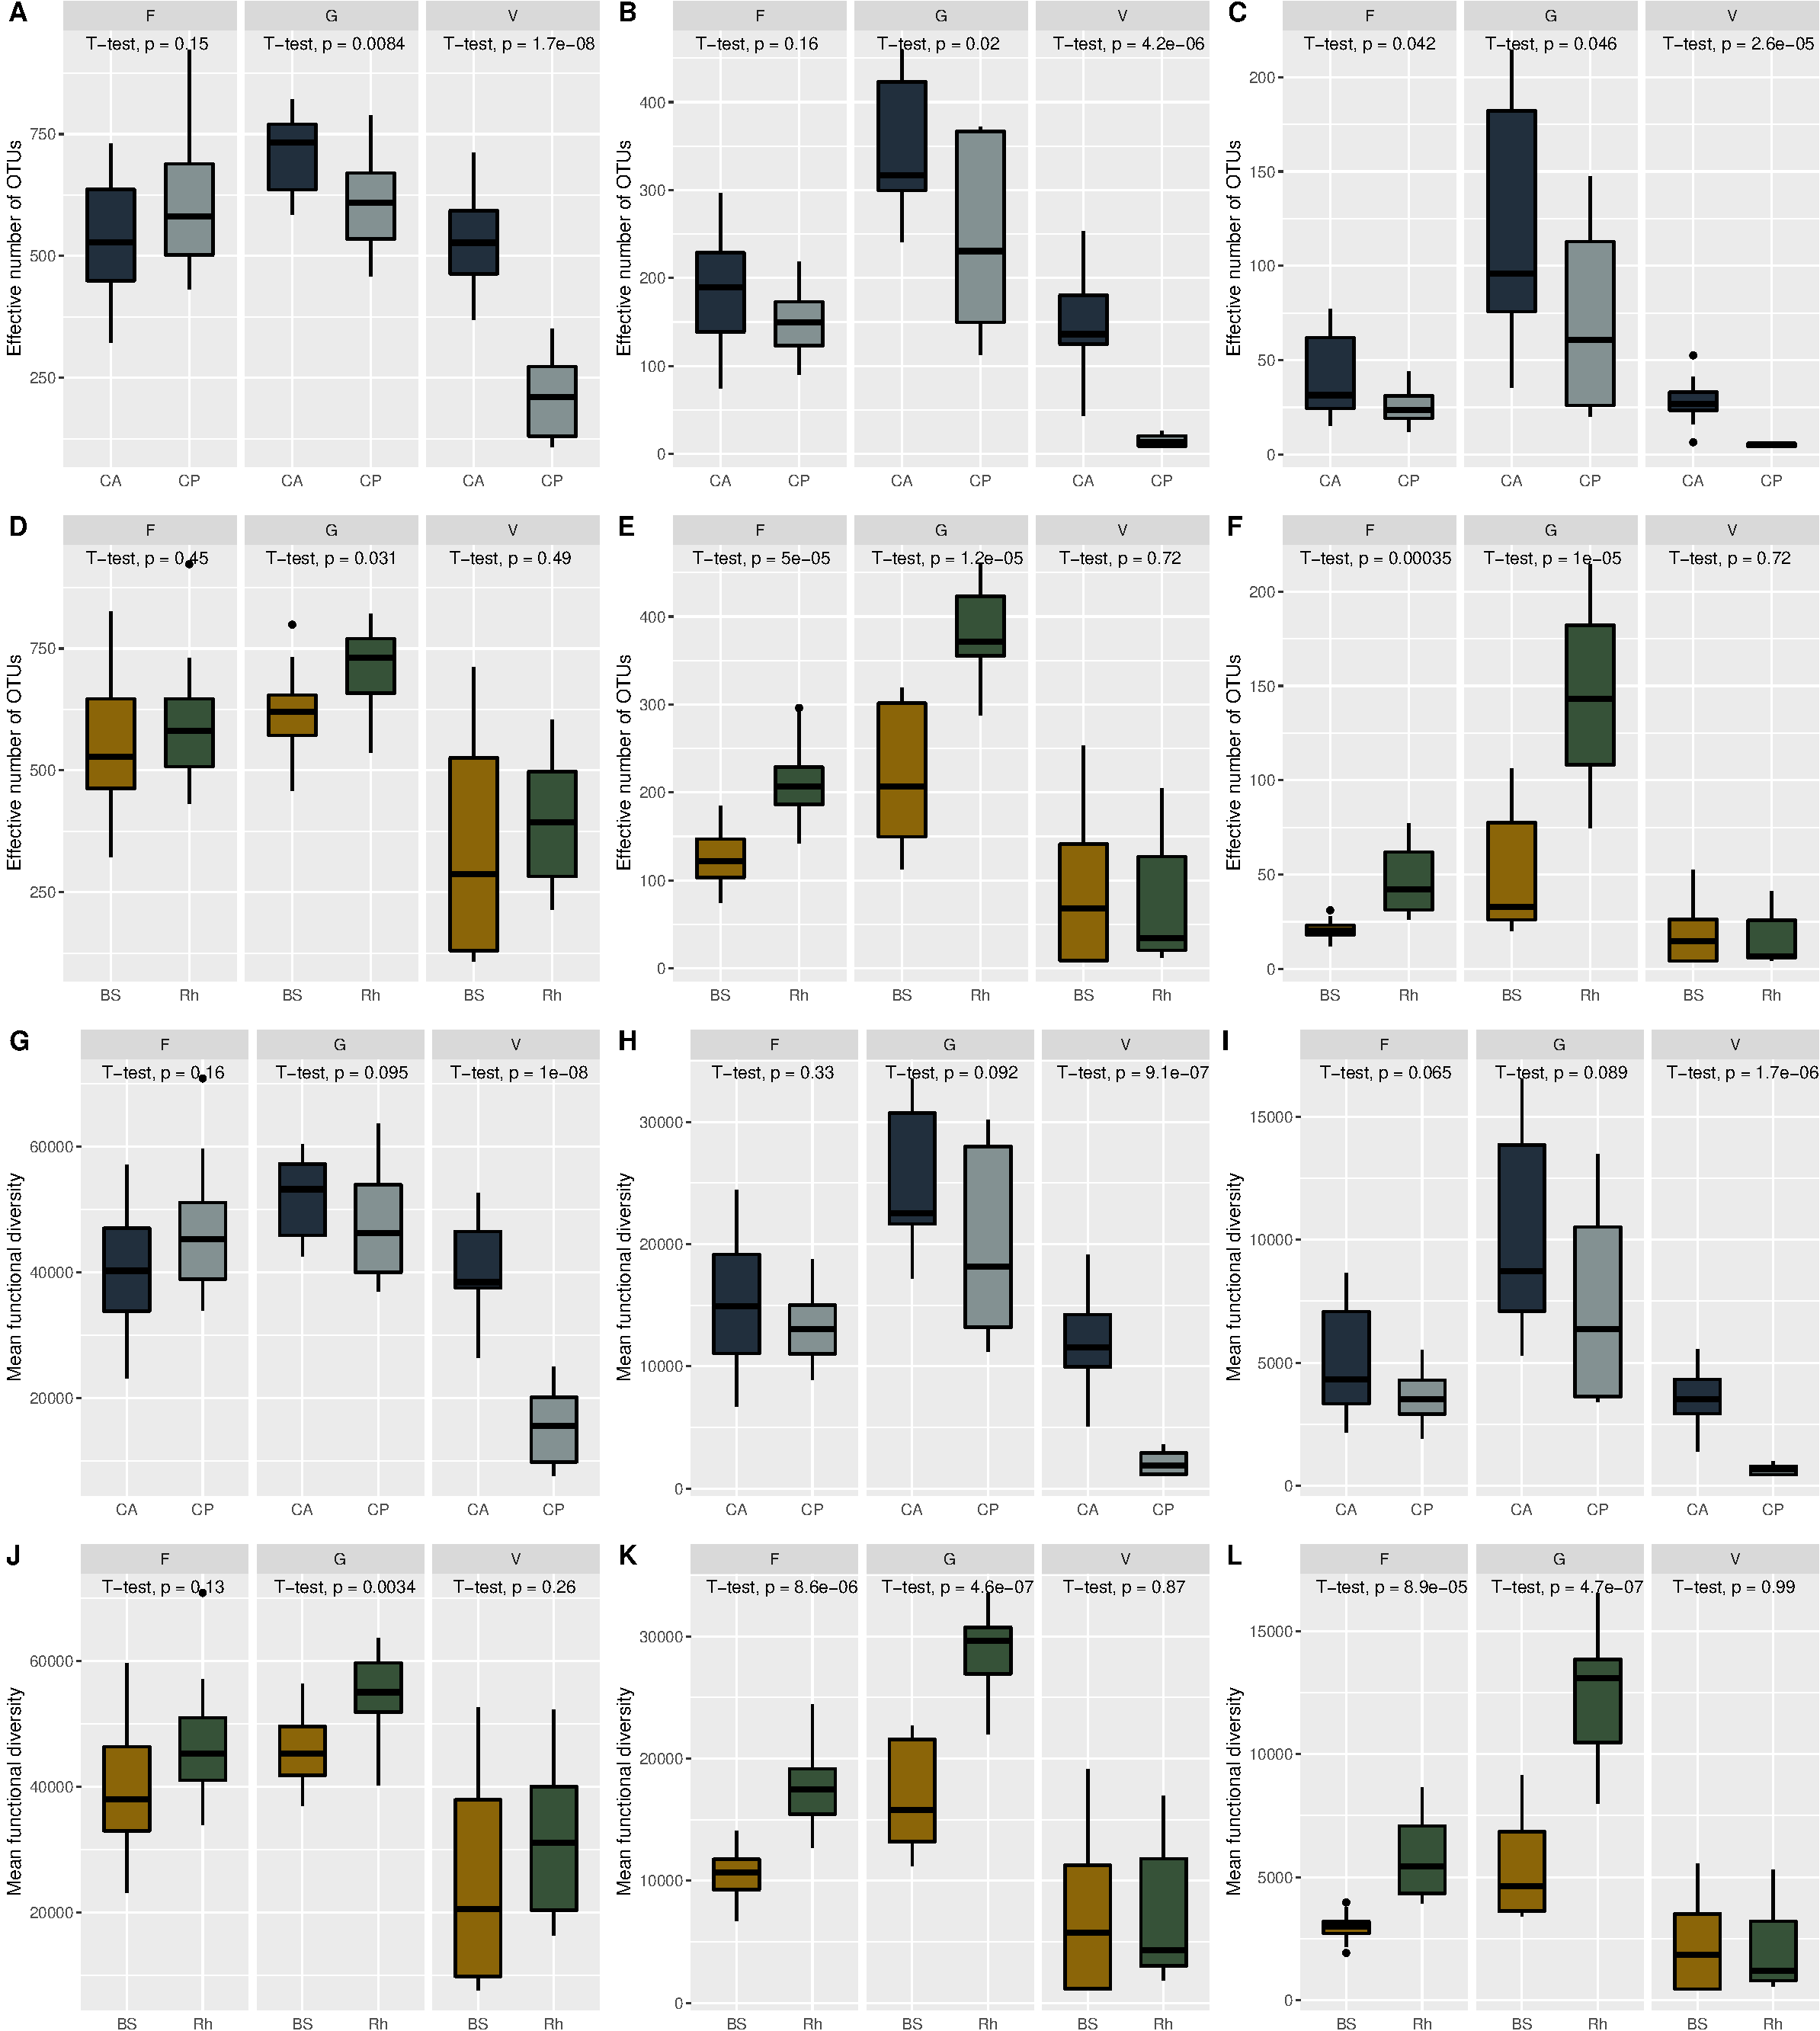
\includegraphics{Doc_pdf_files/figure-latex/unnamed-chunk-14-1} \end{center}

\begin{Shaded}
\begin{Highlighting}[]
\CommentTok{\#pdf("FigS3\_Div\_block\_by\_stage.pdf", width=16, height=18)}
\CommentTok{\#print(r)}
\CommentTok{\#dev.off()}
\end{Highlighting}
\end{Shaded}

\begin{center}\rule{0.5\linewidth}{0.5pt}\end{center}

\begin{center}\rule{0.5\linewidth}{0.5pt}\end{center}

\hypertarget{iii.-beta-diversity-plot}{%
\section{III. BETA-DIVERSITY PLOT}\label{iii.-beta-diversity-plot}}

\hypertarget{loading-libraries-1}{%
\subsubsection{Loading libraries}\label{loading-libraries-1}}

\begin{Shaded}
\begin{Highlighting}[]
\FunctionTok{library}\NormalTok{(cowplot)}
\FunctionTok{library}\NormalTok{(tidyverse)}
\FunctionTok{library}\NormalTok{(ggpubr)}
\FunctionTok{library}\NormalTok{(circlize)}
\FunctionTok{library}\NormalTok{(viridis)}
\FunctionTok{library}\NormalTok{(RColorBrewer)}
\FunctionTok{library}\NormalTok{(grid)}
\FunctionTok{library}\NormalTok{(ggplot2)}
\end{Highlighting}
\end{Shaded}

\hypertarget{loading-and-formatting-files}{%
\subsubsection{Loading and formatting
files}\label{loading-and-formatting-files}}

\begin{Shaded}
\begin{Highlighting}[]
\NormalTok{beta}\OtherTok{\textless{}{-}} \FunctionTok{read\_tsv}\NormalTok{(}\StringTok{"../Data/beta\_diversity.txt"}\NormalTok{) }\SpecialCharTok{\%\textgreater{}\%} \FunctionTok{mutate}\NormalTok{(}\AttributeTok{qs =} \FunctionTok{case\_when}\NormalTok{(}
\NormalTok{  q }\SpecialCharTok{==} \DecValTok{0}  \SpecialCharTok{\textasciitilde{}} \StringTok{"q=0 (species richness)"}\NormalTok{,}
\NormalTok{  q }\SpecialCharTok{==} \DecValTok{1} \SpecialCharTok{\textasciitilde{}} \StringTok{"q=1 (frequent species)"}\NormalTok{,}
\NormalTok{  q }\SpecialCharTok{==} \DecValTok{2} \SpecialCharTok{\textasciitilde{}} \StringTok{"q=2 (dominant species)"}\NormalTok{)) }\SpecialCharTok{\%\textgreater{}\%} \FunctionTok{rename}\NormalTok{(}\StringTok{"ASVs\_turnover"} \OtherTok{=}\NormalTok{ TurnoverComp)}
\FunctionTok{head}\NormalTok{(beta)}
\end{Highlighting}
\end{Shaded}

\begin{verbatim}
## # A tibble: 6 x 12
##       q ID1   ID2    beta LocalOverlap RegionalOverlap Homogeneity ASVs_turnover
##   <dbl> <chr> <chr> <dbl>        <dbl>           <dbl>       <dbl>         <dbl>
## 1     0 CAFB~ CAFR~  1.66        0.343           0.207       0.207         0.343
## 2     1 CAFB~ CAFR~  1.35        0.572           0.572       0.486         0.654
## 3     2 CAFB~ CAFR~  1.04        0.923           0.960       0.923         0.960
## 4     0 CAFB~ CAFR~  1.63        0.370           0.227       0.227         0.370
## 5     1 CAFB~ CAFR~  1.32        0.598           0.598       0.513         0.678
## 6     2 CAFB~ CAFR~  1.09        0.828           0.906       0.828         0.906
## # ... with 4 more variables: Comparison <chr>, PlotCompare <chr>, Type <chr>,
## #   qs <chr>
\end{verbatim}

\hypertarget{treatment-plot}{%
\subsubsection{Treatment plot}\label{treatment-plot}}

\begin{Shaded}
\begin{Highlighting}[]
\NormalTok{ann\_text\_treatment}\OtherTok{\textless{}{-}}\FunctionTok{data.frame}\NormalTok{(}
  \AttributeTok{Comparison=}\FunctionTok{c}\NormalTok{(}\StringTok{"CA\_BSvsRh"}\NormalTok{, }\StringTok{"CA\_BSvsRh"}\NormalTok{, }\StringTok{"CA\_BSvsRh"}\NormalTok{),}
  \StringTok{"ASVs\_turnover"}\OtherTok{=}\FunctionTok{c}\NormalTok{(}\DecValTok{1}\NormalTok{,}\DecValTok{1}\NormalTok{,}\DecValTok{1}\NormalTok{),}
  \AttributeTok{qs=}\FunctionTok{c}\NormalTok{(}\StringTok{"q=0 (species richness)"}\NormalTok{,}\StringTok{"q=1 (frequent species)"}\NormalTok{,}\StringTok{"q=2 (dominant species)"}\NormalTok{),}
  \AttributeTok{label=}\FunctionTok{c}\NormalTok{(}\StringTok{"p\textless{}0.001"}\NormalTok{,}\StringTok{"p=0.399"}\NormalTok{, }\StringTok{"p=0.365"}\NormalTok{)) }\CommentTok{\#tittles and positiong in y axis}

\NormalTok{beta\_treatment}\OtherTok{\textless{}{-}}\NormalTok{ beta }\SpecialCharTok{\%\textgreater{}\%}
  \FunctionTok{filter}\NormalTok{(}\FunctionTok{str\_detect}\NormalTok{(Comparison, }\StringTok{\textquotesingle{}\^{}CA|\^{}CP\textquotesingle{}}\NormalTok{))}\SpecialCharTok{\%\textgreater{}\%} \FunctionTok{ggplot}\NormalTok{(}
    \FunctionTok{aes}\NormalTok{(}\AttributeTok{y=}\StringTok{\textasciigrave{}}\AttributeTok{ASVs\_turnover}\StringTok{\textasciigrave{}}\NormalTok{,}\AttributeTok{x=}\NormalTok{Comparison,  }\AttributeTok{fill=}\NormalTok{Comparison)) }\SpecialCharTok{+}
  \FunctionTok{geom\_boxplot}\NormalTok{(}\AttributeTok{position=}\FunctionTok{position\_dodge}\NormalTok{(}\DecValTok{1}\NormalTok{), }\AttributeTok{outlier.shape =} \ConstantTok{NA}\NormalTok{, }\AttributeTok{color=}\StringTok{"black"}\NormalTok{,}
               \AttributeTok{width=}\FloatTok{0.6}\NormalTok{)}\SpecialCharTok{+}\FunctionTok{theme\_bw}\NormalTok{()}\SpecialCharTok{+}
  \FunctionTok{labs}\NormalTok{(}\AttributeTok{y =} \StringTok{"Proportion of ASVs turnover"}\NormalTok{)}\SpecialCharTok{+}
  \FunctionTok{facet\_grid}\NormalTok{(}\SpecialCharTok{\textasciitilde{}}\NormalTok{qs, }\AttributeTok{scales =} \StringTok{"free"}\NormalTok{)}\SpecialCharTok{+}
  \FunctionTok{theme}\NormalTok{(}\AttributeTok{panel.spacing=}\FunctionTok{unit}\NormalTok{(}\DecValTok{1}\NormalTok{,}\StringTok{"lines"}\NormalTok{),}
        \CommentTok{\# strip.background=element\_rect(color="grey30", fill="gray90"),}
        \CommentTok{\# panel.border=element\_rect(color="black"),}
        \CommentTok{\#strip.text.x = element\_text(}
        \CommentTok{\#  size = 12, color = "black", face = "bold"),}
        \AttributeTok{strip.text.x =} \FunctionTok{element\_text}\NormalTok{(}\AttributeTok{size =} \DecValTok{10}\NormalTok{),}
        \AttributeTok{axis.text =}  \FunctionTok{element\_text}\NormalTok{(}\AttributeTok{colour =} \StringTok{"black"}\NormalTok{, }\AttributeTok{size =} \DecValTok{10}\NormalTok{),}
        \AttributeTok{axis.ticks.x=}\FunctionTok{element\_blank}\NormalTok{(), }
        \AttributeTok{axis.title.x =} \FunctionTok{element\_blank}\NormalTok{(), }
        \AttributeTok{legend.title =} \FunctionTok{element\_blank}\NormalTok{(),}
        \AttributeTok{axis.title.y =} \FunctionTok{element\_text}\NormalTok{(}\AttributeTok{size =} \DecValTok{14}\NormalTok{),}
        \CommentTok{\# legend.text = element\_text(size=16), }
        \CommentTok{\# axis.text.x = element\_blank(),}
        \AttributeTok{panel.grid.major =} \FunctionTok{element\_blank}\NormalTok{(), }\AttributeTok{panel.grid.minor =} \FunctionTok{element\_blank}\NormalTok{(),}
        \CommentTok{\# legend.position = c(0.6,0.8), }
        \AttributeTok{legend.direction =} \StringTok{"vertical"}\NormalTok{ ,}
        \AttributeTok{legend.position =} \StringTok{"none"}\NormalTok{)}\SpecialCharTok{+}\FunctionTok{scale\_fill\_manual}\NormalTok{(}\AttributeTok{values =} \FunctionTok{c}\NormalTok{(}\StringTok{"\#212F3D"}\NormalTok{,}\StringTok{"\#839192"}\NormalTok{))}\SpecialCharTok{+}  
  \FunctionTok{geom\_text}\NormalTok{(}\AttributeTok{data =}\NormalTok{ ann\_text\_treatment,}\AttributeTok{label=}\NormalTok{ann\_text\_treatment}\SpecialCharTok{$}\NormalTok{label)}
\NormalTok{beta\_treatment}
\end{Highlighting}
\end{Shaded}

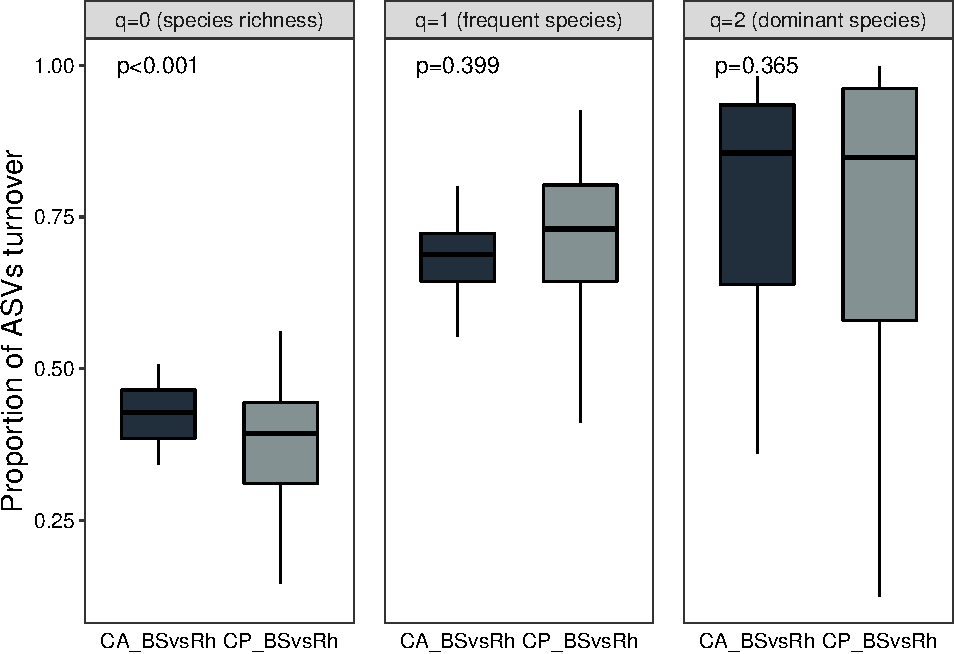
\includegraphics{Doc_pdf_files/figure-latex/unnamed-chunk-18-1.pdf}

\begin{Shaded}
\begin{Highlighting}[]
\CommentTok{\#pdf("fig\_beta\_treatment.pdf", width=6, height=3)}
\CommentTok{\#print(beta\_treatment)}
\CommentTok{\#dev.off()}
\end{Highlighting}
\end{Shaded}

\hypertarget{soil-plot}{%
\subsubsection{Soil Plot}\label{soil-plot}}

\begin{Shaded}
\begin{Highlighting}[]
\NormalTok{ann\_text\_soil}\OtherTok{\textless{}{-}}\FunctionTok{data.frame}\NormalTok{(}
  \AttributeTok{Comparison=}\FunctionTok{c}\NormalTok{(}\StringTok{"BS\_CPvsCA"}\NormalTok{, }\StringTok{"BS\_CPvsCA"}\NormalTok{, }\StringTok{"BS\_CPvsCA"}\NormalTok{),}
  \StringTok{"ASVs\_turnover"}\OtherTok{=}\FunctionTok{c}\NormalTok{(}\DecValTok{1}\NormalTok{,}\DecValTok{1}\NormalTok{,}\DecValTok{1}\NormalTok{),}
  \AttributeTok{qs=}\FunctionTok{c}\NormalTok{(}\StringTok{"q=0 (species richness)"}\NormalTok{,}\StringTok{"q=1 (frequent species)"}\NormalTok{,}\StringTok{"q=2 (dominant species)"}\NormalTok{),}
  \AttributeTok{label=}\FunctionTok{c}\NormalTok{(}\StringTok{"p\textless{}0.001"}\NormalTok{,}\StringTok{"p\textless{}0.001"}\NormalTok{, }\StringTok{"p\textless{}0.001"}\NormalTok{)) }\CommentTok{\#tittles and positiong in y axis}

\NormalTok{beta\_soil}\OtherTok{\textless{}{-}}\NormalTok{ beta }\SpecialCharTok{\%\textgreater{}\%}
  \FunctionTok{filter}\NormalTok{(}\SpecialCharTok{!}\FunctionTok{str\_detect}\NormalTok{(Comparison, }\StringTok{\textquotesingle{}\^{}CA|\^{}CP\textquotesingle{}}\NormalTok{))}\SpecialCharTok{\%\textgreater{}\%} \FunctionTok{ggplot}\NormalTok{(}
    \FunctionTok{aes}\NormalTok{(}\AttributeTok{y=}\StringTok{\textasciigrave{}}\AttributeTok{ASVs\_turnover}\StringTok{\textasciigrave{}}\NormalTok{,}\AttributeTok{x=}\NormalTok{Comparison,  }\AttributeTok{fill=}\NormalTok{Comparison)) }\SpecialCharTok{+}
  \FunctionTok{geom\_boxplot}\NormalTok{(}\AttributeTok{position=}\FunctionTok{position\_dodge}\NormalTok{(}\DecValTok{1}\NormalTok{), }\AttributeTok{outlier.shape =} \ConstantTok{NA}\NormalTok{, }\AttributeTok{color=}\StringTok{"black"}\NormalTok{,}
               \AttributeTok{width=}\FloatTok{0.6}\NormalTok{)}\SpecialCharTok{+}\FunctionTok{theme\_bw}\NormalTok{()}\SpecialCharTok{+}
  \FunctionTok{labs}\NormalTok{(}\AttributeTok{y =} \StringTok{"Proportion of ASVs turnover"}\NormalTok{)}\SpecialCharTok{+}
  \FunctionTok{facet\_grid}\NormalTok{(}\SpecialCharTok{\textasciitilde{}}\NormalTok{qs, }\AttributeTok{scales =} \StringTok{"free"}\NormalTok{)}\SpecialCharTok{+}
  \FunctionTok{theme}\NormalTok{(}\AttributeTok{panel.spacing=}\FunctionTok{unit}\NormalTok{(}\DecValTok{1}\NormalTok{,}\StringTok{"lines"}\NormalTok{),}
        \CommentTok{\# strip.background=element\_rect(color="grey30", fill="gray90"),}
        \CommentTok{\# panel.border=element\_rect(color="black"),}
        \CommentTok{\#strip.text.x = element\_text(}
        \CommentTok{\#  size = 12, color = "black", face = "bold"),}
        \AttributeTok{strip.text.x =} \FunctionTok{element\_text}\NormalTok{(}\AttributeTok{size =} \DecValTok{10}\NormalTok{),}
        \AttributeTok{axis.text =}  \FunctionTok{element\_text}\NormalTok{(}\AttributeTok{colour =} \StringTok{"black"}\NormalTok{, }\AttributeTok{size =} \DecValTok{10}\NormalTok{),}
        \AttributeTok{axis.ticks.x=}\FunctionTok{element\_blank}\NormalTok{(), }
        \AttributeTok{axis.title.x =} \FunctionTok{element\_blank}\NormalTok{(), }
        \AttributeTok{legend.title =} \FunctionTok{element\_blank}\NormalTok{(),}
        \AttributeTok{axis.title.y =} \FunctionTok{element\_text}\NormalTok{(}\AttributeTok{size =} \DecValTok{14}\NormalTok{),}
        \CommentTok{\# legend.text = element\_text(size=16), }
        \CommentTok{\# axis.text.x = element\_blank(),}
        \AttributeTok{panel.grid.major =} \FunctionTok{element\_blank}\NormalTok{(), }\AttributeTok{panel.grid.minor =} \FunctionTok{element\_blank}\NormalTok{(),}
        \CommentTok{\# legend.position = c(0.6,0.8), }
        \AttributeTok{legend.direction =} \StringTok{"vertical"}\NormalTok{ ,}
        \AttributeTok{legend.position =} \StringTok{"none"}\NormalTok{)}\SpecialCharTok{+}\FunctionTok{scale\_fill\_manual}\NormalTok{(}\AttributeTok{values =} \FunctionTok{c}\NormalTok{(}\StringTok{"darkgoldenrod4"}\NormalTok{, }\StringTok{"\#365238"}\NormalTok{))}\SpecialCharTok{+}  
  \FunctionTok{geom\_text}\NormalTok{(}\AttributeTok{data =}\NormalTok{ ann\_text\_soil,}\AttributeTok{label=}\NormalTok{ann\_text\_soil}\SpecialCharTok{$}\NormalTok{label)}
\NormalTok{beta\_soil}
\end{Highlighting}
\end{Shaded}

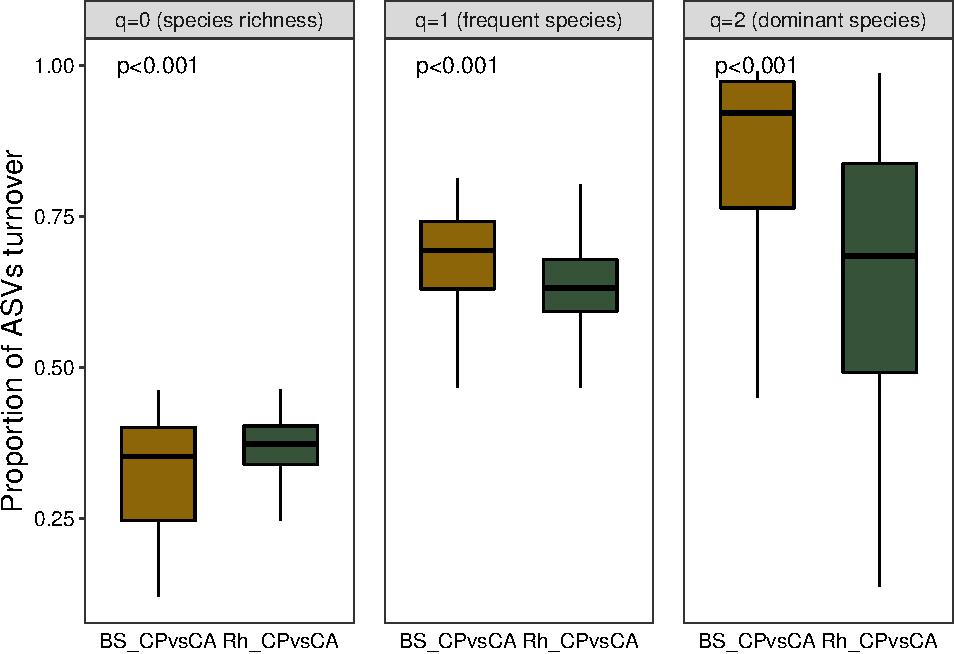
\includegraphics{Doc_pdf_files/figure-latex/unnamed-chunk-19-1.pdf}

\begin{Shaded}
\begin{Highlighting}[]
\CommentTok{\#pdf("fig\_beta\_soil.pdf", width=6, height=3)}
\CommentTok{\#print(beta\_soil)}
\CommentTok{\#dev.off()}
\end{Highlighting}
\end{Shaded}

\hypertarget{iv.-soil-figure}{%
\section{IV. SOIL FIGURE}\label{iv.-soil-figure}}

\hypertarget{loading-libraries-2}{%
\subsubsection{Loading libraries}\label{loading-libraries-2}}

\begin{Shaded}
\begin{Highlighting}[]
\FunctionTok{library}\NormalTok{(cowplot)}
\FunctionTok{library}\NormalTok{(tidyverse)}
\FunctionTok{library}\NormalTok{(ggpubr)}
\FunctionTok{library}\NormalTok{(ComplexHeatmap)}
\FunctionTok{library}\NormalTok{(circlize)}
\FunctionTok{library}\NormalTok{(viridis)}
\FunctionTok{library}\NormalTok{(RColorBrewer)}
\FunctionTok{library}\NormalTok{(grid)}
\FunctionTok{library}\NormalTok{(CoDaSeq)}
\FunctionTok{library}\NormalTok{(ggplot2)}
\FunctionTok{require}\NormalTok{(compositions) }\CommentTok{\# exploratory d ata analysis of compositional data}
\FunctionTok{require}\NormalTok{(zCompositions) }\CommentTok{\# used for 0 substitution}
\FunctionTok{require}\NormalTok{(ALDEx2) }\CommentTok{\# used for per{-}OTU comparisons}
\FunctionTok{library}\NormalTok{(CoDaSeq)}
\FunctionTok{library}\NormalTok{(ggrepel)}
\end{Highlighting}
\end{Shaded}

\hypertarget{loadings-files-and-barplot-text-annotations}{%
\subsubsection{Loadings files and Barplot Text
annotations}\label{loadings-files-and-barplot-text-annotations}}

\begin{Shaded}
\begin{Highlighting}[]
\NormalTok{alpha}\OtherTok{\textless{}{-}} \FunctionTok{read.table}\NormalTok{(}\StringTok{"../Data/alpha\_diversity"}\NormalTok{) }\SpecialCharTok{\%\textgreater{}\%} \FunctionTok{gather}\NormalTok{(}
\NormalTok{  q0}\SpecialCharTok{:}\NormalTok{q4, }\AttributeTok{key =} \StringTok{"q"}\NormalTok{, }\AttributeTok{value =} \StringTok{"value"}\NormalTok{) }\SpecialCharTok{\%\textgreater{}\%} \FunctionTok{filter}\NormalTok{(}
\NormalTok{    q }\SpecialCharTok{\%in\%} \FunctionTok{c}\NormalTok{(}\StringTok{"q0"}\NormalTok{, }\StringTok{"q1"}\NormalTok{, }\StringTok{"q2"}\NormalTok{))}\SpecialCharTok{\%\textgreater{}\%}\FunctionTok{mutate}\NormalTok{(}\AttributeTok{qs=} \FunctionTok{case\_when}\NormalTok{(}
  \FunctionTok{str\_detect}\NormalTok{(q, }\StringTok{"q0"}\NormalTok{) }\SpecialCharTok{\textasciitilde{}} \StringTok{"q=0 (species richness)"}\NormalTok{,}
  \FunctionTok{str\_detect}\NormalTok{(q, }\StringTok{"q1"}\NormalTok{) }\SpecialCharTok{\textasciitilde{}} \StringTok{"q=1 (frequent species)"}\NormalTok{,}
  \FunctionTok{str\_detect}\NormalTok{(q, }\StringTok{"q2"}\NormalTok{) }\SpecialCharTok{\textasciitilde{}} \StringTok{"q=2 (dominant species)"}\NormalTok{))}
\FunctionTok{head}\NormalTok{(alpha)}
\end{Highlighting}
\end{Shaded}

\begin{verbatim}
##   Practice Soil Practice.Location Stage Age Plant Plot ExpUnit  q value
## 1       CA   BS             CA.BS     F   1     1   18 CA.BS.F q0   426
## 2       CA   BS             CA.BS     F   1     2   18 CA.BS.F q0   646
## 3       CA   BS             CA.BS     F   1     3   18 CA.BS.F q0   510
## 4       CA   BS             CA.BS     F   1     1   59 CA.BS.F q0   546
## 5       CA   BS             CA.BS     F   1     2   59 CA.BS.F q0   391
## 6       CA   BS             CA.BS     F   1     3   59 CA.BS.F q0   322
##                       qs
## 1 q=0 (species richness)
## 2 q=0 (species richness)
## 3 q=0 (species richness)
## 4 q=0 (species richness)
## 5 q=0 (species richness)
## 6 q=0 (species richness)
\end{verbatim}

\begin{Shaded}
\begin{Highlighting}[]
\NormalTok{func}\OtherTok{\textless{}{-}} \FunctionTok{read.table}\NormalTok{(}\StringTok{"../Data/func\_MDq.txt"}\NormalTok{) }\SpecialCharTok{\%\textgreater{}\%} \FunctionTok{gather}\NormalTok{(}
\NormalTok{  MD\_q0}\SpecialCharTok{:}\NormalTok{MD\_q2, }\AttributeTok{key =} \StringTok{"q"}\NormalTok{, }\AttributeTok{value =} \StringTok{"value"}\NormalTok{)}\SpecialCharTok{\%\textgreater{}\%}\FunctionTok{mutate}\NormalTok{(}\AttributeTok{fs=} \FunctionTok{case\_when}\NormalTok{(}
  \FunctionTok{str\_detect}\NormalTok{(q, }\StringTok{"q0"}\NormalTok{) }\SpecialCharTok{\textasciitilde{}} \StringTok{"q=0 (species richness)"}\NormalTok{,}
  \FunctionTok{str\_detect}\NormalTok{(q, }\StringTok{"q1"}\NormalTok{) }\SpecialCharTok{\textasciitilde{}} \StringTok{"q=1 (frequent species)"}\NormalTok{,}
  \FunctionTok{str\_detect}\NormalTok{(q, }\StringTok{"q2"}\NormalTok{) }\SpecialCharTok{\textasciitilde{}} \StringTok{"q=2 (dominant species)"}\NormalTok{))}
\FunctionTok{head}\NormalTok{(func) }
\end{Highlighting}
\end{Shaded}

\begin{verbatim}
##   Practice Soil Practice.Location Stage Age Plant Plot ExpUnit     q    value
## 1       CA   BS             CA.BS     F   1     1   18 CA.BS.F MD_q0 29629.84
## 2       CA   BS             CA.BS     F   1     2   18 CA.BS.F MD_q0 46138.20
## 3       CA   BS             CA.BS     F   1     3   18 CA.BS.F MD_q0 36859.81
## 4       CA   BS             CA.BS     F   1     1   59 CA.BS.F MD_q0 39086.65
## 5       CA   BS             CA.BS     F   1     2   59 CA.BS.F MD_q0 28482.32
## 6       CA   BS             CA.BS     F   1     3   59 CA.BS.F MD_q0 23152.35
##                       fs
## 1 q=0 (species richness)
## 2 q=0 (species richness)
## 3 q=0 (species richness)
## 4 q=0 (species richness)
## 5 q=0 (species richness)
## 6 q=0 (species richness)
\end{verbatim}

\begin{Shaded}
\begin{Highlighting}[]
\CommentTok{\#df with the p values to show in the figures}
\NormalTok{ann\_text}\OtherTok{\textless{}{-}}\FunctionTok{data.frame}\NormalTok{(}\AttributeTok{Soil=}\FunctionTok{c}\NormalTok{(}\StringTok{"BS"}\NormalTok{, }\StringTok{"BS"}\NormalTok{, }\StringTok{"BS"}\NormalTok{),}\AttributeTok{value=}\FunctionTok{c}\NormalTok{(}\DecValTok{800}\NormalTok{,}\DecValTok{350}\NormalTok{,}\DecValTok{150}\NormalTok{),}
\AttributeTok{qs=}\FunctionTok{c}\NormalTok{(}\StringTok{"q=0 (species richness)"}\NormalTok{,}\StringTok{"q=1 (frequent species)"}\NormalTok{,}
\StringTok{"q=2 (dominant species)"}\NormalTok{),}\AttributeTok{label=}\FunctionTok{c}\NormalTok{(}\StringTok{"p=0.157"}\NormalTok{,}\StringTok{"p=0.001"}\NormalTok{, }\StringTok{"p\textless{}0.0001"}\NormalTok{))}
\CommentTok{\#tittles and position in y axis}


\NormalTok{ann\_text\_f}\OtherTok{\textless{}{-}}\FunctionTok{data.frame}\NormalTok{(}\AttributeTok{Soil=}\FunctionTok{c}\NormalTok{(}\StringTok{"BS"}\NormalTok{, }\StringTok{"BS"}\NormalTok{, }\StringTok{"BS"}\NormalTok{),}\AttributeTok{value=}\FunctionTok{c}\NormalTok{(}\DecValTok{60000}\NormalTok{,}\DecValTok{30000}\NormalTok{,}\DecValTok{10000}\NormalTok{),}
\AttributeTok{fs=}\FunctionTok{c}\NormalTok{(}\StringTok{"q=0 (species richness)"}\NormalTok{,}\StringTok{"q=1 (frequent species)"}\NormalTok{,}
\StringTok{"q=2 (dominant species)"}\NormalTok{),}\AttributeTok{label=}\FunctionTok{c}\NormalTok{(}\StringTok{"p=0.075"}\NormalTok{,}\StringTok{"p\textless{}0.0001"}\NormalTok{, }\StringTok{"p\textless{}0.0001"}\NormalTok{)) }
\CommentTok{\#tittles and position in y axis}
\end{Highlighting}
\end{Shaded}

\hypertarget{barplots-alpha-and-functional-diversity}{%
\subsubsection{Barplots alpha and functional
diversity}\label{barplots-alpha-and-functional-diversity}}

\begin{Shaded}
\begin{Highlighting}[]
\CommentTok{\#Alpha diversity barplot soil}
\NormalTok{boxplot\_soil}\OtherTok{\textless{}{-}}\NormalTok{alpha }\SpecialCharTok{\%\textgreater{}\%} 
  \FunctionTok{ggbarplot}\NormalTok{(}\AttributeTok{x=}\StringTok{"qs"}\NormalTok{, }\AttributeTok{y=}\StringTok{"value"}\NormalTok{, }\AttributeTok{fill =} \StringTok{"Soil"}\NormalTok{, }\AttributeTok{add =} \StringTok{"mean\_se"}\NormalTok{, }
            \AttributeTok{position =} \FunctionTok{position\_dodge}\NormalTok{())}\SpecialCharTok{+}
    \FunctionTok{theme\_bw}\NormalTok{()}\SpecialCharTok{+}
  \FunctionTok{labs}\NormalTok{(}\AttributeTok{y =} \StringTok{"Effective number of ASVs"}\NormalTok{)}\SpecialCharTok{+}
  \FunctionTok{facet\_wrap}\NormalTok{(}\SpecialCharTok{\textasciitilde{}}\NormalTok{qs, }\AttributeTok{scales =} \StringTok{"free"}\NormalTok{, }\AttributeTok{dir =} \StringTok{"v"}\NormalTok{)}\SpecialCharTok{+}
  \FunctionTok{theme}\NormalTok{(}\AttributeTok{panel.spacing=}\FunctionTok{unit}\NormalTok{(}\DecValTok{1}\NormalTok{,}\StringTok{"lines"}\NormalTok{),}
        \AttributeTok{strip.text.x =} \FunctionTok{element\_text}\NormalTok{(}\AttributeTok{size =} \DecValTok{10}\NormalTok{),}
        \AttributeTok{axis.text =}  \FunctionTok{element\_text}\NormalTok{(}\AttributeTok{colour =} \StringTok{"black"}\NormalTok{, }\AttributeTok{size =} \DecValTok{10}\NormalTok{),}
        \AttributeTok{axis.ticks.x=}\FunctionTok{element\_blank}\NormalTok{(), }
        \AttributeTok{legend.title =} \FunctionTok{element\_text}\NormalTok{(}\AttributeTok{size =} \DecValTok{14}\NormalTok{),}
        \AttributeTok{legend.text =} \FunctionTok{element\_text}\NormalTok{(}\AttributeTok{size=}\DecValTok{14}\NormalTok{), }
        \AttributeTok{axis.text.x =} \FunctionTok{element\_blank}\NormalTok{(),}
        \AttributeTok{panel.grid.major =} \FunctionTok{element\_blank}\NormalTok{(), }\AttributeTok{panel.grid.minor =} \FunctionTok{element\_blank}\NormalTok{(),}
        \AttributeTok{legend.direction =} \StringTok{"horizontal"}\NormalTok{ ,}
        \AttributeTok{legend.position =} \StringTok{"top"}\NormalTok{)}\SpecialCharTok{+}\FunctionTok{scale\_fill\_manual}\NormalTok{(}
          \AttributeTok{values =} \FunctionTok{c}\NormalTok{(}\StringTok{"darkgoldenrod4"}\NormalTok{, }\StringTok{"\#365238"}\NormalTok{))}\SpecialCharTok{+} \FunctionTok{labs}\NormalTok{(}\AttributeTok{fill =} \StringTok{"Soil"}\NormalTok{)}

\NormalTok{boxplot\_soil}\OtherTok{\textless{}{-}}\NormalTok{boxplot\_soil }\SpecialCharTok{+}  \FunctionTok{geom\_text}\NormalTok{(}\AttributeTok{data =}\NormalTok{ ann\_text,}\AttributeTok{label=}\NormalTok{ann\_text}\SpecialCharTok{$}\NormalTok{label)}

\NormalTok{boxplot\_soil}
\end{Highlighting}
\end{Shaded}

\begin{center}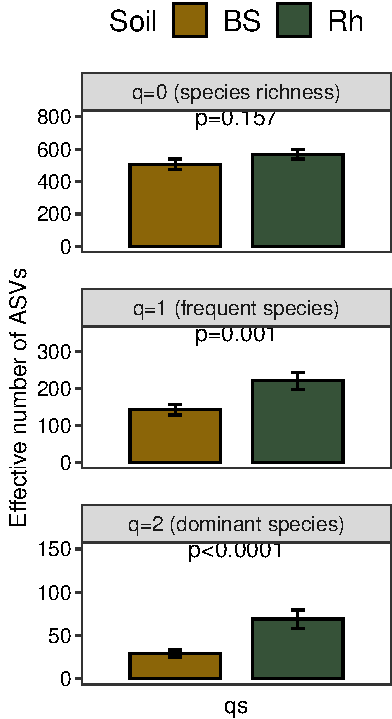
\includegraphics{Doc_pdf_files/figure-latex/unnamed-chunk-22-1} \end{center}

\begin{Shaded}
\begin{Highlighting}[]
\CommentTok{\#Functional diversity barplot soil}
\NormalTok{boxplot\_soil\_f}\OtherTok{\textless{}{-}}\NormalTok{func }\SpecialCharTok{\%\textgreater{}\%} 
  \FunctionTok{ggbarplot}\NormalTok{(}\AttributeTok{x=}\StringTok{"fs"}\NormalTok{, }\AttributeTok{y=}\StringTok{"value"}\NormalTok{, }\AttributeTok{fill =} \StringTok{"Soil"}\NormalTok{, }\AttributeTok{add =} \StringTok{"mean\_se"}\NormalTok{, }
            \AttributeTok{position =} \FunctionTok{position\_dodge}\NormalTok{())}\SpecialCharTok{+}
  \FunctionTok{theme\_bw}\NormalTok{()}\SpecialCharTok{+}
  \FunctionTok{labs}\NormalTok{(}\AttributeTok{y =} \StringTok{"Mean functional diversity"}\NormalTok{)}\SpecialCharTok{+}
  \FunctionTok{facet\_wrap}\NormalTok{(}\SpecialCharTok{\textasciitilde{}}\NormalTok{fs, }\AttributeTok{scales =} \StringTok{"free"}\NormalTok{, }\AttributeTok{dir =} \StringTok{"v"}\NormalTok{)}\SpecialCharTok{+}
  \FunctionTok{theme}\NormalTok{(}\AttributeTok{panel.spacing=}\FunctionTok{unit}\NormalTok{(}\DecValTok{1}\NormalTok{,}\StringTok{"lines"}\NormalTok{),}
        \AttributeTok{strip.text.x =} \FunctionTok{element\_text}\NormalTok{(}\AttributeTok{size =} \DecValTok{10}\NormalTok{),}
        \AttributeTok{axis.text =}  \FunctionTok{element\_text}\NormalTok{(}\AttributeTok{colour =} \StringTok{"black"}\NormalTok{, }\AttributeTok{size =} \DecValTok{10}\NormalTok{),}
        \AttributeTok{axis.ticks.x=}\FunctionTok{element\_blank}\NormalTok{(), }
        \AttributeTok{legend.title =} \FunctionTok{element\_text}\NormalTok{(}\AttributeTok{size =} \DecValTok{14}\NormalTok{),}
        \AttributeTok{legend.text =} \FunctionTok{element\_text}\NormalTok{(}\AttributeTok{size=}\DecValTok{14}\NormalTok{), }
        \AttributeTok{axis.text.x =} \FunctionTok{element\_blank}\NormalTok{(),}
        \AttributeTok{panel.grid.major =} \FunctionTok{element\_blank}\NormalTok{(), }\AttributeTok{panel.grid.minor =} \FunctionTok{element\_blank}\NormalTok{(),}
        \AttributeTok{legend.direction =} \StringTok{"horizontal"}\NormalTok{ ,}
        \AttributeTok{legend.position =} \StringTok{"top"}\NormalTok{)}\SpecialCharTok{+}\FunctionTok{scale\_fill\_manual}\NormalTok{(}\AttributeTok{values =} \FunctionTok{c}\NormalTok{(}
          \StringTok{"darkgoldenrod4"}\NormalTok{, }\StringTok{"\#365238"}\NormalTok{))}\SpecialCharTok{+} \FunctionTok{labs}\NormalTok{(}\AttributeTok{fill =} \StringTok{"Soil"}\NormalTok{)}

\NormalTok{boxplot\_soil\_f}\OtherTok{\textless{}{-}}\NormalTok{boxplot\_soil\_f }\SpecialCharTok{+}  \FunctionTok{geom\_text}\NormalTok{(}\AttributeTok{data =}\NormalTok{ ann\_text\_f,}\AttributeTok{label=}\NormalTok{ann\_text\_f}\SpecialCharTok{$}\NormalTok{label)}

\NormalTok{boxplot\_soil\_f}
\end{Highlighting}
\end{Shaded}

\begin{center}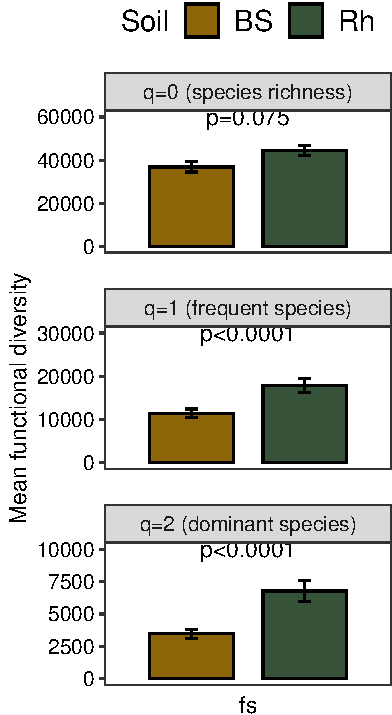
\includegraphics{Doc_pdf_files/figure-latex/unnamed-chunk-22-2} \end{center}

\begin{Shaded}
\begin{Highlighting}[]
\CommentTok{\#ggsave(\textquotesingle{}./fig\_alpha\_soil.png\textquotesingle{},}
 \CommentTok{\#   width = 2.5, height = 5, dpi = 300, plot = boxplot\_soil)}

\CommentTok{\#ggsave(\textquotesingle{}./fig\_func\_soil.png\textquotesingle{},}
 \CommentTok{\#      width = 2.5, height = 5, dpi = 300, plot = boxplot\_soil\_f)}

\CommentTok{\#pdf("fig\_alpha\_soil.pdf", width=2.5, height=5)}
\CommentTok{\#print(boxplot\_soil)}
\CommentTok{\#dev.off()}
\CommentTok{\#pdf("fig\_func\_soil.pdf", width=2.5, height=5)}
\CommentTok{\#print(boxplot\_soil\_f)}
\CommentTok{\#dev.off()}
\end{Highlighting}
\end{Shaded}

\hypertarget{aldex-results-heatmap-from-soil}{%
\subsubsection{Aldex results heatmap from
Soil}\label{aldex-results-heatmap-from-soil}}

\begin{Shaded}
\begin{Highlighting}[]
\CommentTok{\#file to heatmap}
\NormalTok{aldex\_all\_dif}\OtherTok{\textless{}{-}} \FunctionTok{read\_tsv}\NormalTok{(}\StringTok{"../Data/aldex\_soil.tsv"}\NormalTok{)}

\NormalTok{my\_fun }\OtherTok{\textless{}{-}} \ControlFlowTok{function}\NormalTok{(x) \{ }
\NormalTok{  x }\SpecialCharTok{\%\textgreater{}\%} \FunctionTok{separate}\NormalTok{(}
    \StringTok{"Taxon"}\NormalTok{, }\FunctionTok{c}\NormalTok{(}\StringTok{"k"}\NormalTok{, }\StringTok{"phylum"}\NormalTok{,}\StringTok{"c"}\NormalTok{, }\StringTok{"o"}\NormalTok{,}\StringTok{"f"}\NormalTok{,}\StringTok{"g"}\NormalTok{),}
    \AttributeTok{sep =} \StringTok{"}\SpecialCharTok{\textbackslash{}\textbackslash{}}\StringTok{;"}\NormalTok{, }\AttributeTok{remove =}\NormalTok{ F) }\SpecialCharTok{\%\textgreater{}\%}\NormalTok{ dplyr}\SpecialCharTok{::}\FunctionTok{select}\NormalTok{(}
\NormalTok{      Taxon, p.value, effect, diff.btw, rab.win}\FloatTok{.0}\NormalTok{, rab.win}\FloatTok{.1}\NormalTok{, phylum, }
      \StringTok{"FeatureID"}\OtherTok{=}\StringTok{"Feature.ID"}\NormalTok{ )}\SpecialCharTok{\%\textgreater{}\%} 
    \FunctionTok{drop\_na}\NormalTok{(.)}\SpecialCharTok{\%\textgreater{}\%} 
    \FunctionTok{rownames\_to\_column}\NormalTok{(}\AttributeTok{var=}\StringTok{"rows"}\NormalTok{)}\SpecialCharTok{\%\textgreater{}\%}       
    \FunctionTok{mutate\_all}\NormalTok{(}\FunctionTok{funs}\NormalTok{(}\FunctionTok{str\_replace}\NormalTok{(., }\StringTok{"k\_\_Bacteria;"}\NormalTok{, }\StringTok{""}\NormalTok{)))}\SpecialCharTok{\%\textgreater{}\%}
    \FunctionTok{mutate\_all}\NormalTok{(}\FunctionTok{funs}\NormalTok{(}\FunctionTok{str\_replace}\NormalTok{(., }\StringTok{"; c\_\_; o\_\_; f\_\_; g\_\_; s\_\_"}\NormalTok{, }\StringTok{""}\NormalTok{)))}\SpecialCharTok{\%\textgreater{}\%} 
    \FunctionTok{mutate\_all}\NormalTok{(}\FunctionTok{funs}\NormalTok{(}\FunctionTok{str\_replace}\NormalTok{(., }\StringTok{"; o\_\_; f\_\_; g\_\_; s\_\_"}\NormalTok{, }\StringTok{""}\NormalTok{)))}\SpecialCharTok{\%\textgreater{}\%} 
    \FunctionTok{mutate\_all}\NormalTok{(}\FunctionTok{funs}\NormalTok{(}\FunctionTok{str\_replace}\NormalTok{(., }\StringTok{"; f\_\_; g\_\_; s\_\_"}\NormalTok{, }\StringTok{""}\NormalTok{)))}\SpecialCharTok{\%\textgreater{}\%}
    \FunctionTok{mutate\_all}\NormalTok{(}\FunctionTok{funs}\NormalTok{(}\FunctionTok{str\_replace}\NormalTok{(., }\StringTok{"; g\_\_; s\_\_"}\NormalTok{, }\StringTok{""}\NormalTok{)))}\SpecialCharTok{\%\textgreater{}\%}
    \FunctionTok{mutate\_all}\NormalTok{(}\FunctionTok{funs}\NormalTok{(}\FunctionTok{str\_replace}\NormalTok{(., }\StringTok{"; s\_\_"}\NormalTok{, }\StringTok{""}\NormalTok{)))}\SpecialCharTok{\%\textgreater{}\%}\FunctionTok{mutate}\NormalTok{(}
      \AttributeTok{tax=} \FunctionTok{str\_extract}\NormalTok{(Taxon, }\StringTok{"[\^{}\_]+$"}\NormalTok{)) }\SpecialCharTok{\%\textgreater{}\%}\FunctionTok{mutate}\NormalTok{(}
        \AttributeTok{taxo =} \FunctionTok{paste}\NormalTok{(rows,}\StringTok{"\_"}\NormalTok{,tax))}\SpecialCharTok{\%\textgreater{}\%} \FunctionTok{mutate\_at}\NormalTok{(}
          \FunctionTok{c}\NormalTok{(}\DecValTok{3}\SpecialCharTok{:}\DecValTok{7}\NormalTok{), as.numeric) }\SpecialCharTok{\%\textgreater{}\%}
    \FunctionTok{mutate\_at}\NormalTok{(}\FunctionTok{c}\NormalTok{(}\DecValTok{3}\NormalTok{), }\FunctionTok{funs}\NormalTok{(}\AttributeTok{p.Value =} \FunctionTok{case\_when}\NormalTok{(}
\NormalTok{      . }\SpecialCharTok{\textless{}=} \FloatTok{0.001} \SpecialCharTok{\textasciitilde{}} \StringTok{"\textless{}0.001"}\NormalTok{,}
\NormalTok{      . }\SpecialCharTok{\textgreater{}}  \FloatTok{0.001} \SpecialCharTok{\&}\NormalTok{ .  }\SpecialCharTok{\textless{}=} \FloatTok{0.01} \SpecialCharTok{\textasciitilde{}} \StringTok{"\textless{}0.01"}\NormalTok{,}
\NormalTok{      . }\SpecialCharTok{\textgreater{}}  \FloatTok{0.01} \SpecialCharTok{\&}\NormalTok{ .  }\SpecialCharTok{\textless{}=} \FloatTok{0.05} \SpecialCharTok{\textasciitilde{}} \StringTok{"\textless{}0.05"}\NormalTok{)))}\SpecialCharTok{\%\textgreater{}\%}
    \FunctionTok{arrange}\NormalTok{(diff.btw)}\SpecialCharTok{\%\textgreater{}\%}\FunctionTok{column\_to\_rownames}\NormalTok{(}
      \AttributeTok{var =} \StringTok{"taxo"}\NormalTok{)}\SpecialCharTok{\%\textgreater{}\%} \FunctionTok{mutate\_at}\NormalTok{(}\FunctionTok{c}\NormalTok{(}\DecValTok{8}\NormalTok{),}\FunctionTok{funs}\NormalTok{(}\FunctionTok{str\_replace}\NormalTok{(., }\StringTok{"p\_\_"}\NormalTok{, }\StringTok{""}\NormalTok{)))}
\NormalTok{\}}
\CommentTok{\#We are going to multiplicate for {-}1 in order to change }
\CommentTok{\#the direction of the figure (e.g, bulk soil first and then rhizosphere)}

\NormalTok{annotation\_heatmap }\OtherTok{\textless{}{-}} \FunctionTok{my\_fun}\NormalTok{(aldex\_all\_dif) }\SpecialCharTok{\%\textgreater{}\%} \FunctionTok{mutate}\NormalTok{(}
  \AttributeTok{diff.btw2 =}\NormalTok{ diff.btw}\SpecialCharTok{*{-}}\DecValTok{1}\NormalTok{, }\AttributeTok{effect2 =}\NormalTok{ effect}\SpecialCharTok{*{-}}\DecValTok{1}\NormalTok{ ) }\SpecialCharTok{\%\textgreater{}\%} \FunctionTok{arrange}\NormalTok{(diff.btw2) }\SpecialCharTok{\%\textgreater{}\%} \FunctionTok{mutate}\NormalTok{(}
    \AttributeTok{taxo=} \FunctionTok{paste}\NormalTok{(rows,tax, }\AttributeTok{sep =} \StringTok{"\_"}\NormalTok{))}
\NormalTok{data\_heatmap}\OtherTok{\textless{}{-}}\NormalTok{ annotation\_heatmap}\SpecialCharTok{\%\textgreater{}\%}\NormalTok{dplyr}\SpecialCharTok{::}\FunctionTok{select}\NormalTok{(rab.win}\FloatTok{.1}\NormalTok{, rab.win}\FloatTok{.0}\NormalTok{) }\SpecialCharTok{\%\textgreater{}\%} \FunctionTok{rename}\NormalTok{(}
  \AttributeTok{rab.win.Rh=}\NormalTok{rab.win}\FloatTok{.0}\NormalTok{ , }\AttributeTok{rab.win.Bs=}\NormalTok{rab.win}\FloatTok{.1}\NormalTok{)}


\NormalTok{color\_heatmap}\OtherTok{=} \FunctionTok{colorRamp2}\NormalTok{(}\FunctionTok{seq}\NormalTok{(}\FunctionTok{min}\NormalTok{(data\_heatmap), }\FunctionTok{max}\NormalTok{(data\_heatmap), }\AttributeTok{length =} \DecValTok{5}\NormalTok{), }\FunctionTok{c}\NormalTok{(}
  \StringTok{"\#0000FF"}\NormalTok{,}\StringTok{"\#5499C7"}\NormalTok{, }\StringTok{"\#DAE7E4"}\NormalTok{,  }\StringTok{"red"}\NormalTok{, }\StringTok{"\#FF0000"}\NormalTok{))}

\CommentTok{\#Annotation Phylum}
\NormalTok{cols\_ann }\OtherTok{\textless{}{-}} \FunctionTok{list}\NormalTok{(}\StringTok{\textquotesingle{}phylum\textquotesingle{}} \OtherTok{=} \FunctionTok{c}\NormalTok{(}
  \StringTok{" Acidobacteria"} \OtherTok{=} \StringTok{\textquotesingle{}red2\textquotesingle{}}\NormalTok{,}
  \StringTok{" Actinobacteria"} \OtherTok{=} \StringTok{\textquotesingle{}royalblue\textquotesingle{}}\NormalTok{,}
  \StringTok{" Bacteroidetes"}\OtherTok{=}\StringTok{"yellow"}\NormalTok{,}
  \StringTok{" Chloroflexi"} \OtherTok{=}\StringTok{"pink"}\NormalTok{,}
  \StringTok{" Firmicutes"}\OtherTok{=} \StringTok{"green"}\NormalTok{,}
  \StringTok{" Gemmatimonadetes"} \OtherTok{=} \StringTok{"black"}\NormalTok{,}
  \StringTok{" Nitrospirae"} \OtherTok{=}\StringTok{"purple"}\NormalTok{,}
  \StringTok{" Planctomycetes"} \OtherTok{=}\StringTok{"dark green"}\NormalTok{,}
  \StringTok{" Proteobacteria"}  \OtherTok{=}\StringTok{"gray"}\NormalTok{,}
  \StringTok{" Verrucomicrobia"} \OtherTok{=}\StringTok{"brown"}\NormalTok{))}
\NormalTok{colAnn }\OtherTok{\textless{}{-}} \FunctionTok{HeatmapAnnotation}\NormalTok{(}\AttributeTok{phylum =}\NormalTok{ annotation\_heatmap}\SpecialCharTok{$}\NormalTok{phylum,}
                            \AttributeTok{which =} \StringTok{\textquotesingle{}row\textquotesingle{}}\NormalTok{,}
                            \AttributeTok{col =}\NormalTok{ cols\_ann,}
                            \AttributeTok{show\_legend =}\NormalTok{ T)}


\CommentTok{\#Annotation pvalue}

\NormalTok{cols\_pvalue }\OtherTok{\textless{}{-}} \FunctionTok{list}\NormalTok{(}\StringTok{\textquotesingle{}p{-}value\textquotesingle{}} \OtherTok{=} \FunctionTok{c}\NormalTok{(}\StringTok{"\textless{}0.001"} \OtherTok{=} \StringTok{\textquotesingle{}\#AB0000\textquotesingle{}}\NormalTok{,}
                                  \StringTok{"\textless{}0.01"} \OtherTok{=} \StringTok{\textquotesingle{}\#FF0000\textquotesingle{}}\NormalTok{,}
                                  \StringTok{"\textless{}0.05"}\OtherTok{=}\StringTok{"\#FFB6B6"}\NormalTok{))}

\NormalTok{annP2 }\OtherTok{=} \FunctionTok{HeatmapAnnotation}\NormalTok{(}\StringTok{"p{-}value"} \OtherTok{=}\NormalTok{ annotation\_heatmap}\SpecialCharTok{$}\NormalTok{p.Value,}
                          \AttributeTok{which =} \StringTok{"row"}\NormalTok{, }\AttributeTok{col =}\NormalTok{ cols\_pvalue,}
                          \AttributeTok{show\_legend =}\NormalTok{ T)}\CommentTok{\#, gp = gpar(col = "white"))}


\CommentTok{\#Annotation effect size}
\NormalTok{effect\_col\_fun }\OtherTok{=}\FunctionTok{colorRamp2}\NormalTok{(}\FunctionTok{c}\NormalTok{(}\SpecialCharTok{{-}}\FloatTok{1.5}\NormalTok{, }\DecValTok{0}\NormalTok{, }\FloatTok{1.5}\NormalTok{), }\FunctionTok{c}\NormalTok{(}\StringTok{"lightsalmon4"}\NormalTok{, }\StringTok{"white"}\NormalTok{, }\StringTok{"lightseagreen"}\NormalTok{))}

\NormalTok{annEffect }\OtherTok{=} \FunctionTok{HeatmapAnnotation}\NormalTok{(}\StringTok{"effect{-}size"} \OtherTok{=}\NormalTok{ annotation\_heatmap}\SpecialCharTok{$}\NormalTok{effect2,}
                              \AttributeTok{which =} \StringTok{"row"}\NormalTok{, }\AttributeTok{col =} \FunctionTok{list}\NormalTok{(}\StringTok{"effect{-}size"} \OtherTok{=}\NormalTok{ effect\_col\_fun),}
                              \AttributeTok{show\_legend =}\NormalTok{ T, }
                              \AttributeTok{gp =} \FunctionTok{gpar}\NormalTok{(}\AttributeTok{col =} \StringTok{"white"}\NormalTok{))}
\CommentTok{\# gap = unit(10, "cm"))}

\CommentTok{\#Annotation barplot}
\NormalTok{bardif}\OtherTok{=} \FunctionTok{rowAnnotation}\NormalTok{(}\StringTok{"difference }\SpecialCharTok{\textbackslash{}n}\StringTok{ between groups"} \OtherTok{=} \FunctionTok{anno\_barplot}\NormalTok{(}
\NormalTok{  annotation\_heatmap}\SpecialCharTok{$}\NormalTok{diff.btw2, }\AttributeTok{width =} \FunctionTok{unit}\NormalTok{(}\DecValTok{4}\NormalTok{, }\StringTok{"cm"}\NormalTok{)))}

\CommentTok{\#Annotation taxonomy}


\NormalTok{labels }\OtherTok{=} \FunctionTok{c}\NormalTok{(}\StringTok{"RB41"}\NormalTok{, }\StringTok{"iii1{-}15"}\NormalTok{, }\StringTok{"Bacillus"}\NormalTok{, }\StringTok{"Halomonas"}\NormalTok{, }\FunctionTok{rep}\NormalTok{(}\StringTok{""}\NormalTok{, }\DecValTok{7}\NormalTok{),}\StringTok{"Burkholderiaceae"}\NormalTok{,}
           \StringTok{"Comamonadaceae"}\NormalTok{,}\StringTok{"Comamonadaceae"}\NormalTok{, }\StringTok{"Xanthomonadales"}\NormalTok{, }\StringTok{"Oxalobacteraceae"}\NormalTok{,}
           \StringTok{"Rhodospirillaceae"}\NormalTok{, }\StringTok{"Solibacterales"}\NormalTok{,}\StringTok{"Comamonadaceae"}\NormalTok{, }\StringTok{"Rhizobiales"}\NormalTok{,}\StringTok{"Rhizobiales"}\NormalTok{,}
           \StringTok{"Comamonadaceae"}\NormalTok{ , }\StringTok{"Oxalobacteraceae"}\NormalTok{)}

\CommentTok{\#Heat map}
\NormalTok{heatmap\_aldex\_soil}\OtherTok{\textless{}{-}}\NormalTok{ComplexHeatmap}\SpecialCharTok{::}  \FunctionTok{Heatmap}\NormalTok{(data\_heatmap, }\AttributeTok{col =}\NormalTok{ color\_heatmap, }
\AttributeTok{row\_dend\_reorder =}\NormalTok{ F, }\AttributeTok{width =} \FunctionTok{ncol}\NormalTok{(data\_heatmap)}\SpecialCharTok{*}\FunctionTok{unit}\NormalTok{(}\DecValTok{1}\NormalTok{, }\StringTok{"cm"}\NormalTok{),}
\AttributeTok{height =} \FunctionTok{ncol}\NormalTok{(data\_heatmap)}\SpecialCharTok{*}\FunctionTok{unit}\NormalTok{(}\FloatTok{2.2}\NormalTok{, }\StringTok{"cm"}\NormalTok{),}
\AttributeTok{left\_annotation =}  \FunctionTok{c}\NormalTok{(annP2, annEffect, colAnn),}
\AttributeTok{cluster\_column\_slices =}\NormalTok{ F,}
\AttributeTok{heatmap\_legend\_param =} \FunctionTok{list}\NormalTok{(}\AttributeTok{direction =} \StringTok{"horizontal"}\NormalTok{ ),}
\AttributeTok{right\_annotation =} \FunctionTok{c}\NormalTok{(bardif),}
\AttributeTok{column\_split =} \FunctionTok{c}\NormalTok{(}\StringTok{"BS"}\NormalTok{, }\StringTok{"Rh"}\NormalTok{),}
\AttributeTok{cluster\_rows =}\NormalTok{ F,}
\AttributeTok{cluster\_columns =}\NormalTok{ F,}
\AttributeTok{column\_km =} \DecValTok{1}\NormalTok{, }
\AttributeTok{column\_title\_gp =} \FunctionTok{gpar}\NormalTok{(}\AttributeTok{fill =} \FunctionTok{c}\NormalTok{(}\StringTok{"darkgoldenrod4"}\NormalTok{, }\StringTok{"\#365238"}\NormalTok{ ), }\AttributeTok{col=}\StringTok{"white"}\NormalTok{),}
\AttributeTok{border =}\NormalTok{ F, }\AttributeTok{column\_gap =} \FunctionTok{unit}\NormalTok{(}\FloatTok{0.5}\NormalTok{, }\StringTok{"mm"}\NormalTok{), }\AttributeTok{row\_dend\_side =} \StringTok{"left"}\NormalTok{,}
\AttributeTok{row\_names\_side =} \StringTok{"right"}\NormalTok{, }\AttributeTok{show\_row\_names =}\NormalTok{ F,}
\AttributeTok{rect\_gp =} \FunctionTok{gpar}\NormalTok{(}\AttributeTok{col =} \StringTok{"white"}\NormalTok{, }\AttributeTok{lwd =} \FloatTok{0.2}\NormalTok{), }
\AttributeTok{row\_names\_gp =} \FunctionTok{gpar}\NormalTok{(}\AttributeTok{fontface =}\StringTok{"italic"}\NormalTok{, }\AttributeTok{fontsize=}\DecValTok{10}\NormalTok{),}
\AttributeTok{show\_column\_names =}\NormalTok{ F, }\AttributeTok{name =} \StringTok{"rab.Win"}\NormalTok{)}\SpecialCharTok{+}
\FunctionTok{rowAnnotation}\NormalTok{(}\AttributeTok{labels =} \FunctionTok{anno\_text}\NormalTok{(labels, }\AttributeTok{which =} \StringTok{"row"}\NormalTok{,}
\FunctionTok{gpar}\NormalTok{(}\AttributeTok{col =} \StringTok{"black"}\NormalTok{, }\AttributeTok{fontsize =} \DecValTok{6}\NormalTok{)), }
\AttributeTok{width =} \FunctionTok{unit}\NormalTok{(}\DecValTok{2}\NormalTok{, }\StringTok{"cm"}\NormalTok{))}

\NormalTok{heatmap\_aldex\_soil}
\end{Highlighting}
\end{Shaded}

\begin{center}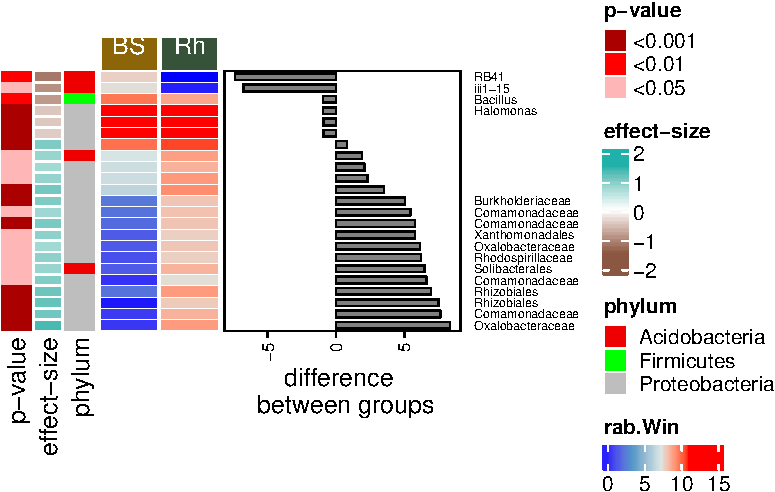
\includegraphics{Doc_pdf_files/figure-latex/unnamed-chunk-23-1} \end{center}

\begin{Shaded}
\begin{Highlighting}[]
\CommentTok{\#pdf("fig\_aldex\_soil.pdf", width=6, height=5)}
\CommentTok{\#print(heatmap\_aldex\_soil)}
\CommentTok{\#dev.off()}
\end{Highlighting}
\end{Shaded}

\hypertarget{pca-plot}{%
\subsubsection{PCA plot}\label{pca-plot}}

\begin{Shaded}
\begin{Highlighting}[]
\CommentTok{\#loading files and formatting}

\NormalTok{d.pro}\FloatTok{.0}\OtherTok{\textless{}{-}} \FunctionTok{read\_tsv}\NormalTok{(}\StringTok{"../Data/otutable.tsv"}\NormalTok{)}\SpecialCharTok{\%\textgreater{}\%} \FunctionTok{column\_to\_rownames}\NormalTok{(}\AttributeTok{var =} \StringTok{"\#OTU ID"}\NormalTok{)}
\NormalTok{meta}\OtherTok{\textless{}{-}}\FunctionTok{read\_tsv}\NormalTok{(}\StringTok{"../Data/metadata.tsv"}\NormalTok{)}

\NormalTok{meta}\SpecialCharTok{$}\NormalTok{Soil}\OtherTok{\textless{}{-}} \FunctionTok{factor}\NormalTok{(meta}\SpecialCharTok{$}\NormalTok{Soil\_sample,}
                   \AttributeTok{levels =} \FunctionTok{c}\NormalTok{( }\StringTok{"bulksoil"}\NormalTok{, }\StringTok{"Rhizosphere"}\NormalTok{),}
                   \AttributeTok{labels =} \FunctionTok{c}\NormalTok{(}\StringTok{"BS"}\NormalTok{, }\StringTok{"Rh"}\NormalTok{))}

\NormalTok{tax}\OtherTok{\textless{}{-}}\FunctionTok{read\_tsv}\NormalTok{(}\StringTok{"../Data/taxonomy.tsv"}\NormalTok{) }\SpecialCharTok{\%\textgreater{}\%}\NormalTok{ dplyr}\SpecialCharTok{::}\FunctionTok{select}\NormalTok{(}\SpecialCharTok{{-}}\NormalTok{Confidence)}\SpecialCharTok{\%\textgreater{}\%}
  \FunctionTok{mutate\_all}\NormalTok{(}\FunctionTok{funs}\NormalTok{(}\FunctionTok{str\_replace}\NormalTok{(., }\StringTok{"k\_\_Bacteria;"}\NormalTok{, }\StringTok{""}\NormalTok{)))}\SpecialCharTok{\%\textgreater{}\%} 
  \FunctionTok{mutate\_all}\NormalTok{(}\FunctionTok{funs}\NormalTok{(}\FunctionTok{str\_replace}\NormalTok{(., }\StringTok{"p\_\_"}\NormalTok{, }\StringTok{""}\NormalTok{)))}\SpecialCharTok{\%\textgreater{}\%} 
  \FunctionTok{mutate\_all}\NormalTok{(}\FunctionTok{funs}\NormalTok{(}\FunctionTok{str\_replace}\NormalTok{(., }\StringTok{"c\_\_"}\NormalTok{, }\StringTok{""}\NormalTok{)))}\SpecialCharTok{\%\textgreater{}\%} 
  \FunctionTok{mutate\_all}\NormalTok{(}\FunctionTok{funs}\NormalTok{(}\FunctionTok{str\_replace}\NormalTok{(., }\StringTok{"o\_\_"}\NormalTok{, }\StringTok{""}\NormalTok{)))}\SpecialCharTok{\%\textgreater{}\%} 
  \FunctionTok{mutate\_all}\NormalTok{(}\FunctionTok{funs}\NormalTok{(}\FunctionTok{str\_replace}\NormalTok{(., }\StringTok{"f\_\_"}\NormalTok{, }\StringTok{""}\NormalTok{)))}\SpecialCharTok{\%\textgreater{}\%} 
  \FunctionTok{mutate\_all}\NormalTok{(}\FunctionTok{funs}\NormalTok{(}\FunctionTok{str\_replace}\NormalTok{(., }\StringTok{"g\_\_"}\NormalTok{, }\StringTok{""}\NormalTok{)))}\SpecialCharTok{\%\textgreater{}\%} 
  \FunctionTok{mutate\_all}\NormalTok{(}\FunctionTok{funs}\NormalTok{(}\FunctionTok{str\_replace}\NormalTok{(., }\StringTok{"s\_\_"}\NormalTok{, }\StringTok{""}\NormalTok{)))}\SpecialCharTok{\%\textgreater{}\%} 
  \FunctionTok{mutate\_all}\NormalTok{(}\FunctionTok{funs}\NormalTok{(}\FunctionTok{str\_replace}\NormalTok{(., }\StringTok{"; ; ;"}\NormalTok{, }\StringTok{""}\NormalTok{)))}\SpecialCharTok{\%\textgreater{}\%} 
  \FunctionTok{mutate\_all}\NormalTok{(}\FunctionTok{funs}\NormalTok{(}\FunctionTok{str\_replace}\NormalTok{(., }\StringTok{"; ; "}\NormalTok{, }\StringTok{""}\NormalTok{))) }\SpecialCharTok{\%\textgreater{}\%} \FunctionTok{rename}\NormalTok{(}
    \StringTok{"FeatureID"}\OtherTok{=}\StringTok{\textasciigrave{}}\AttributeTok{\#OTU ID}\StringTok{\textasciigrave{}}\NormalTok{, }\AttributeTok{Taxon=}\NormalTok{ taxonomy)}

\NormalTok{tax2}\OtherTok{\textless{}{-}} \FunctionTok{read\_tsv}\NormalTok{(}\StringTok{"../Data/taxonomy.tsv"}\NormalTok{) }\SpecialCharTok{\%\textgreater{}\%}\NormalTok{ dplyr}\SpecialCharTok{::}\FunctionTok{select}\NormalTok{(}
  \SpecialCharTok{{-}}\NormalTok{Confidence) }\SpecialCharTok{\%\textgreater{}\%} \FunctionTok{rename}\NormalTok{(}
    \StringTok{"FeatureID"}\OtherTok{=}\StringTok{\textasciigrave{}}\AttributeTok{\#OTU ID}\StringTok{\textasciigrave{}}\NormalTok{, }\AttributeTok{Taxon=}\NormalTok{ taxonomy)}


\CommentTok{\#transforming data}
\NormalTok{d.pro }\OtherTok{\textless{}{-}} \FunctionTok{cmultRepl}\NormalTok{(}\FunctionTok{t}\NormalTok{(d.pro}\FloatTok{.0}\NormalTok{), }\AttributeTok{method=}\StringTok{"CZM"}\NormalTok{, }\AttributeTok{output=}\StringTok{"p{-}counts"}\NormalTok{)}
\NormalTok{d.clr.abund.codaseq}\OtherTok{\textless{}{-}}\FunctionTok{codaSeq.clr}\NormalTok{(}\AttributeTok{x =}\NormalTok{ d.pro,}\AttributeTok{samples.by.row =}\NormalTok{ F)}

\CommentTok{\#run pca}
\NormalTok{pcx.abund }\OtherTok{\textless{}{-}} \FunctionTok{prcomp}\NormalTok{(d.clr.abund.codaseq)}

\CommentTok{\#labels to pca axis}

\NormalTok{PC1 }\OtherTok{\textless{}{-}} \FunctionTok{paste}\NormalTok{(}\StringTok{"PC1"}\NormalTok{, }\FunctionTok{round}\NormalTok{(}\FunctionTok{sum}\NormalTok{(pcx.abund}\SpecialCharTok{$}\NormalTok{sdev[}\DecValTok{1}\NormalTok{] }\SpecialCharTok{\^{}} \DecValTok{2}\NormalTok{) }\SpecialCharTok{/} \FunctionTok{mvar}\NormalTok{(d.clr.abund.codaseq) }\SpecialCharTok{*} \DecValTok{100}\NormalTok{, }\DecValTok{1}\NormalTok{), }\StringTok{"\%"}\NormalTok{)}
\NormalTok{PC2 }\OtherTok{\textless{}{-}} \FunctionTok{paste}\NormalTok{(}\StringTok{"P21"}\NormalTok{, }\FunctionTok{round}\NormalTok{(}\FunctionTok{sum}\NormalTok{(pcx.abund}\SpecialCharTok{$}\NormalTok{sdev[}\DecValTok{2}\NormalTok{] }\SpecialCharTok{\^{}} \DecValTok{2}\NormalTok{) }\SpecialCharTok{/} \FunctionTok{mvar}\NormalTok{(d.clr.abund.codaseq) }\SpecialCharTok{*} \DecValTok{100}\NormalTok{, }\DecValTok{1}\NormalTok{), }\StringTok{"\%"}\NormalTok{)}


\CommentTok{\#let\textquotesingle{}s choose som of the significant groups from aldex analysis }

\NormalTok{vars\_chosen}\OtherTok{\textless{}{-}} \FunctionTok{c}\NormalTok{(}\StringTok{"14\_RB41"}\NormalTok{, }
                \StringTok{"3\_iii1{-}15"}\NormalTok{,}
                \StringTok{"16\_Oxalobacteraceae"}\NormalTok{ , }
                \StringTok{"11\_Comamonadaceae"}\NormalTok{, }
                \StringTok{"13\_Rhizobiales"}\NormalTok{,}
                \StringTok{"21\_Solibacterales"}\NormalTok{,}
                \StringTok{"20\_Rhodospirillaceae"}\NormalTok{)}
\CommentTok{\#these ones were chosen from before (some aldex significant groups)}

\NormalTok{vars\_to\_choose}\OtherTok{\textless{}{-}}\NormalTok{ annotation\_heatmap }\SpecialCharTok{\%\textgreater{}\%}  \FunctionTok{filter}\NormalTok{(taxo }\SpecialCharTok{\%in\%}\NormalTok{ vars\_chosen)}

\NormalTok{vars\_choosing}\OtherTok{\textless{}{-}} \FunctionTok{data.frame}\NormalTok{(pcx.abund}\SpecialCharTok{$}\NormalTok{rotation) }\SpecialCharTok{\%\textgreater{}\%}  \FunctionTok{rownames\_to\_column}\NormalTok{(}\AttributeTok{var =} \StringTok{"FeatureID"}\NormalTok{)}\SpecialCharTok{\%\textgreater{}\%}   
  \FunctionTok{mutate}\NormalTok{(}\AttributeTok{a=}\FunctionTok{sqrt}\NormalTok{(PC1}\SpecialCharTok{\^{}}\DecValTok{2}\SpecialCharTok{+}\NormalTok{PC2}\SpecialCharTok{\^{}}\DecValTok{2}\NormalTok{)) }\SpecialCharTok{\%\textgreater{}\%}
  \FunctionTok{mutate}\NormalTok{(}\AttributeTok{PC1=}\NormalTok{PC1}\SpecialCharTok{*}\DecValTok{500}\NormalTok{, }\AttributeTok{PC2=}\NormalTok{PC2}\SpecialCharTok{*}\DecValTok{500}\NormalTok{) }\SpecialCharTok{\%\textgreater{}\%} \FunctionTok{left\_join}\NormalTok{(tax2)}\SpecialCharTok{\%\textgreater{}\%}\NormalTok{ dplyr}\SpecialCharTok{::}\FunctionTok{select}\NormalTok{(}
\NormalTok{    Taxon, PC1, PC2, FeatureID)}\SpecialCharTok{\%\textgreater{}\%}\FunctionTok{right\_join}\NormalTok{(vars\_to\_choose, }\AttributeTok{by =} \StringTok{"FeatureID"}\NormalTok{)}

\CommentTok{\#create the base plot with only the arrows}
\NormalTok{pca\_soil\_arrows}\OtherTok{\textless{}{-}} \FunctionTok{ggplot}\NormalTok{() }\SpecialCharTok{+}
  \FunctionTok{theme\_bw}\NormalTok{() }\SpecialCharTok{+}
  \FunctionTok{xlab}\NormalTok{(PC1) }\SpecialCharTok{+}
  \FunctionTok{ylab}\NormalTok{(PC2) }\SpecialCharTok{+}
  \FunctionTok{theme}\NormalTok{(}\AttributeTok{axis.text =} \FunctionTok{element\_text}\NormalTok{(}\AttributeTok{colour =} \StringTok{"black"}\NormalTok{, }\AttributeTok{size =} \DecValTok{14}\NormalTok{),}\CommentTok{\#setting theme}
        \AttributeTok{axis.title =} \FunctionTok{element\_text}\NormalTok{(}\AttributeTok{colour =} \StringTok{"black"}\NormalTok{, }\AttributeTok{size =} \DecValTok{14}\NormalTok{),}
        \AttributeTok{legend.text =} \FunctionTok{element\_text}\NormalTok{(}\AttributeTok{size =} \DecValTok{14}\NormalTok{),}
        \AttributeTok{legend.title =} \FunctionTok{element\_blank}\NormalTok{(), }
        \AttributeTok{legend.position =} \StringTok{"bottom"}\NormalTok{) }\SpecialCharTok{+}
  \FunctionTok{geom\_point}\NormalTok{(                              }\CommentTok{\#individuals}
    \AttributeTok{data=}\FunctionTok{data.frame}\NormalTok{(pcx.abund}\SpecialCharTok{$}\NormalTok{x) }\SpecialCharTok{\%\textgreater{}\%}   \FunctionTok{rownames\_to\_column}\NormalTok{(}\AttributeTok{var =} \StringTok{"SampleID"}\NormalTok{)}\SpecialCharTok{\%\textgreater{}\%}
      \FunctionTok{left\_join}\NormalTok{(meta, }\AttributeTok{by =} \StringTok{"SampleID"}\NormalTok{),}
    \FunctionTok{aes}\NormalTok{(}\AttributeTok{x=}\NormalTok{PC1, }\AttributeTok{y=}\NormalTok{PC2, }\AttributeTok{fill=}\NormalTok{Soil), }
    \AttributeTok{shape=}\DecValTok{21}\NormalTok{, }\AttributeTok{size=}\DecValTok{4}\NormalTok{) }\SpecialCharTok{+}
  \FunctionTok{geom\_vline}\NormalTok{(}\AttributeTok{xintercept =} \DecValTok{0}\NormalTok{, }\AttributeTok{linetype =} \DecValTok{2}\NormalTok{) }\SpecialCharTok{+}   \CommentTok{\#lines{-}cross}
  \FunctionTok{geom\_hline}\NormalTok{(}\AttributeTok{yintercept =} \DecValTok{0}\NormalTok{, }\AttributeTok{linetype =} \DecValTok{2}\NormalTok{) }\SpecialCharTok{+}
  \FunctionTok{scale\_fill\_manual}\NormalTok{(}\AttributeTok{values =} \FunctionTok{c}\NormalTok{(}\StringTok{"darkgoldenrod4"}\NormalTok{, }\StringTok{"\#365238"}\NormalTok{))}\SpecialCharTok{+}
\NormalTok{  ggrepel}\SpecialCharTok{::}\FunctionTok{geom\_label\_repel}\NormalTok{(}\AttributeTok{data =}\NormalTok{ vars\_choosing, }\FunctionTok{aes}\NormalTok{(}\AttributeTok{x=}\NormalTok{PC1, }\AttributeTok{y=}\NormalTok{PC2, }\AttributeTok{label=}\NormalTok{ tax),}
                            \AttributeTok{segment.colour =} \ConstantTok{NA}\NormalTok{, }\AttributeTok{box.padding =} \DecValTok{2}\NormalTok{, }\AttributeTok{fontface=}\StringTok{"italic"}\NormalTok{)}\SpecialCharTok{+}
  \FunctionTok{geom\_segment}\NormalTok{(}\AttributeTok{data =}\NormalTok{ vars\_choosing,  }\CommentTok{\#arrows and names}
               \FunctionTok{aes}\NormalTok{(}\AttributeTok{x=}\DecValTok{0}\NormalTok{, }\AttributeTok{y=}\DecValTok{0}\NormalTok{, }\AttributeTok{xend=}\NormalTok{PC1, }\AttributeTok{yend=}\NormalTok{PC2), }
               \AttributeTok{arrow=}\FunctionTok{arrow}\NormalTok{(}\AttributeTok{length=}\FunctionTok{unit}\NormalTok{(}\FloatTok{0.15}\NormalTok{,}\StringTok{"cm"}\NormalTok{)),}
               \AttributeTok{size=} \FloatTok{0.6}\NormalTok{)}

\NormalTok{pca\_soil\_arrows}
\end{Highlighting}
\end{Shaded}

\begin{center}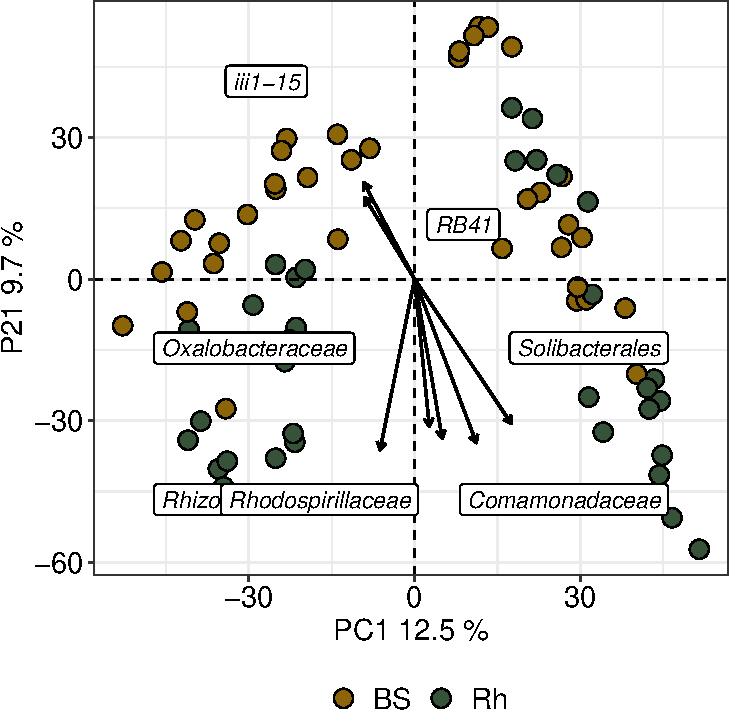
\includegraphics{Doc_pdf_files/figure-latex/unnamed-chunk-24-1} \end{center}

\begin{Shaded}
\begin{Highlighting}[]
\CommentTok{\#pdf("fig\_pca\_soil.pdf", width=5, height=5)}
\CommentTok{\#print(pca\_soil\_arrows)}
\CommentTok{\#dev.off()}
\end{Highlighting}
\end{Shaded}

\hypertarget{v.-treatment-figure}{%
\section{V. TREATMENT FIGURE}\label{v.-treatment-figure}}

\hypertarget{loading-libraries-3}{%
\subsubsection{Loading libraries}\label{loading-libraries-3}}

\begin{Shaded}
\begin{Highlighting}[]
\FunctionTok{library}\NormalTok{(cowplot)}
\FunctionTok{library}\NormalTok{(tidyverse)}
\FunctionTok{library}\NormalTok{(ggpubr)}
\FunctionTok{library}\NormalTok{(ComplexHeatmap)}
\FunctionTok{library}\NormalTok{(circlize)}
\FunctionTok{library}\NormalTok{(viridis)}
\FunctionTok{library}\NormalTok{(RColorBrewer)}
\FunctionTok{library}\NormalTok{(grid)}
\FunctionTok{library}\NormalTok{(CoDaSeq)}
\FunctionTok{library}\NormalTok{(ggplot2)}
\FunctionTok{require}\NormalTok{(compositions) }\CommentTok{\# exploratory d ata analysis of compositional data}
\FunctionTok{require}\NormalTok{(zCompositions) }\CommentTok{\# used for 0 substitution}
\FunctionTok{require}\NormalTok{(ALDEx2) }\CommentTok{\# used for per{-}OTU comparisons}
\FunctionTok{library}\NormalTok{(CoDaSeq)}
\FunctionTok{library}\NormalTok{(ggrepel)}
\end{Highlighting}
\end{Shaded}

\hypertarget{loadings-files-and-barplot-text-annotations-1}{%
\subsubsection{Loadings files and Barplot Text
annotations}\label{loadings-files-and-barplot-text-annotations-1}}

\begin{Shaded}
\begin{Highlighting}[]
\NormalTok{alpha}\OtherTok{\textless{}{-}} \FunctionTok{read.table}\NormalTok{(}\StringTok{"../Data/alpha\_diversity"}\NormalTok{) }\SpecialCharTok{\%\textgreater{}\%} \FunctionTok{gather}\NormalTok{(}
\NormalTok{  q0}\SpecialCharTok{:}\NormalTok{q4, }\AttributeTok{key =} \StringTok{"q"}\NormalTok{, }\AttributeTok{value =} \StringTok{"value"}\NormalTok{) }\SpecialCharTok{\%\textgreater{}\%} \FunctionTok{filter}\NormalTok{(}
\NormalTok{    q }\SpecialCharTok{\%in\%} \FunctionTok{c}\NormalTok{(}\StringTok{"q0"}\NormalTok{, }\StringTok{"q1"}\NormalTok{, }\StringTok{"q2"}\NormalTok{))}\SpecialCharTok{\%\textgreater{}\%}\FunctionTok{mutate}\NormalTok{(}\AttributeTok{qs=} \FunctionTok{case\_when}\NormalTok{(}
  \FunctionTok{str\_detect}\NormalTok{(q, }\StringTok{"q0"}\NormalTok{) }\SpecialCharTok{\textasciitilde{}} \StringTok{"q=0 (species richness)"}\NormalTok{,}
  \FunctionTok{str\_detect}\NormalTok{(q, }\StringTok{"q1"}\NormalTok{) }\SpecialCharTok{\textasciitilde{}} \StringTok{"q=1 (frequent species)"}\NormalTok{,}
  \FunctionTok{str\_detect}\NormalTok{(q, }\StringTok{"q2"}\NormalTok{) }\SpecialCharTok{\textasciitilde{}} \StringTok{"q=2 (dominant species)"}\NormalTok{))}
\FunctionTok{head}\NormalTok{(alpha)}
\end{Highlighting}
\end{Shaded}

\begin{verbatim}
##   Practice Soil Practice.Location Stage Age Plant Plot ExpUnit  q value
## 1       CA   BS             CA.BS     F   1     1   18 CA.BS.F q0   426
## 2       CA   BS             CA.BS     F   1     2   18 CA.BS.F q0   646
## 3       CA   BS             CA.BS     F   1     3   18 CA.BS.F q0   510
## 4       CA   BS             CA.BS     F   1     1   59 CA.BS.F q0   546
## 5       CA   BS             CA.BS     F   1     2   59 CA.BS.F q0   391
## 6       CA   BS             CA.BS     F   1     3   59 CA.BS.F q0   322
##                       qs
## 1 q=0 (species richness)
## 2 q=0 (species richness)
## 3 q=0 (species richness)
## 4 q=0 (species richness)
## 5 q=0 (species richness)
## 6 q=0 (species richness)
\end{verbatim}

\begin{Shaded}
\begin{Highlighting}[]
\NormalTok{func}\OtherTok{\textless{}{-}} \FunctionTok{read.table}\NormalTok{(}\StringTok{"../Data/func\_MDq.txt"}\NormalTok{) }\SpecialCharTok{\%\textgreater{}\%} \FunctionTok{gather}\NormalTok{(}
\NormalTok{  MD\_q0}\SpecialCharTok{:}\NormalTok{MD\_q2, }\AttributeTok{key =} \StringTok{"q"}\NormalTok{, }\AttributeTok{value =} \StringTok{"value"}\NormalTok{)}\SpecialCharTok{\%\textgreater{}\%}\FunctionTok{mutate}\NormalTok{(}\AttributeTok{fs=} \FunctionTok{case\_when}\NormalTok{(}
  \FunctionTok{str\_detect}\NormalTok{(q, }\StringTok{"q0"}\NormalTok{) }\SpecialCharTok{\textasciitilde{}} \StringTok{"q=0 (species richness)"}\NormalTok{,}
  \FunctionTok{str\_detect}\NormalTok{(q, }\StringTok{"q1"}\NormalTok{) }\SpecialCharTok{\textasciitilde{}} \StringTok{"q=1 (frequent species)"}\NormalTok{,}
  \FunctionTok{str\_detect}\NormalTok{(q, }\StringTok{"q2"}\NormalTok{) }\SpecialCharTok{\textasciitilde{}} \StringTok{"q=2 (dominant species)"}\NormalTok{))}
\FunctionTok{head}\NormalTok{(func) }
\end{Highlighting}
\end{Shaded}

\begin{verbatim}
##   Practice Soil Practice.Location Stage Age Plant Plot ExpUnit     q    value
## 1       CA   BS             CA.BS     F   1     1   18 CA.BS.F MD_q0 29629.84
## 2       CA   BS             CA.BS     F   1     2   18 CA.BS.F MD_q0 46138.20
## 3       CA   BS             CA.BS     F   1     3   18 CA.BS.F MD_q0 36859.81
## 4       CA   BS             CA.BS     F   1     1   59 CA.BS.F MD_q0 39086.65
## 5       CA   BS             CA.BS     F   1     2   59 CA.BS.F MD_q0 28482.32
## 6       CA   BS             CA.BS     F   1     3   59 CA.BS.F MD_q0 23152.35
##                       fs
## 1 q=0 (species richness)
## 2 q=0 (species richness)
## 3 q=0 (species richness)
## 4 q=0 (species richness)
## 5 q=0 (species richness)
## 6 q=0 (species richness)
\end{verbatim}

\begin{Shaded}
\begin{Highlighting}[]
\CommentTok{\#df with the p values to show in the figures}
\NormalTok{ann\_text}\OtherTok{\textless{}{-}}\FunctionTok{data.frame}\NormalTok{(}\AttributeTok{Practice=}\FunctionTok{c}\NormalTok{(}\StringTok{"CA"}\NormalTok{, }\StringTok{"CA"}\NormalTok{, }\StringTok{"CA"}\NormalTok{),}\AttributeTok{value=}\FunctionTok{c}\NormalTok{(}\DecValTok{800}\NormalTok{,}\DecValTok{350}\NormalTok{,}\DecValTok{150}\NormalTok{),}
\AttributeTok{qs=}\FunctionTok{c}\NormalTok{(}\StringTok{"q=0 (species richness)"}\NormalTok{,}\StringTok{"q=1 (frequent species)"}\NormalTok{,}
\StringTok{"q=2 (dominant species)"}\NormalTok{),}\AttributeTok{label=}\FunctionTok{c}\NormalTok{(}\StringTok{"p=0.009"}\NormalTok{,}\StringTok{"p=0.002"}\NormalTok{, }\StringTok{"p=0.011"}\NormalTok{)) }
\CommentTok{\#tittles and positiong in y axis}

\NormalTok{ann\_text\_f}\OtherTok{\textless{}{-}}\FunctionTok{data.frame}\NormalTok{(}\AttributeTok{Practice=}\FunctionTok{c}\NormalTok{(}\StringTok{"BS"}\NormalTok{, }\StringTok{"BS"}\NormalTok{, }\StringTok{"BS"}\NormalTok{),}\AttributeTok{value=}\FunctionTok{c}\NormalTok{(}\DecValTok{60000}\NormalTok{,}\DecValTok{30000}\NormalTok{,}\DecValTok{10000}\NormalTok{),}
\AttributeTok{fs=}\FunctionTok{c}\NormalTok{(}\StringTok{"q=0 (species richness)"}\NormalTok{,}\StringTok{"q=1 (frequent species)"}\NormalTok{,}
\StringTok{"q=2 (dominant species)"}\NormalTok{),}\AttributeTok{label=}\FunctionTok{c}\NormalTok{(}\StringTok{"p=0.059"}\NormalTok{,}\StringTok{"p=0.015"}\NormalTok{, }\StringTok{"p=0.026"}\NormalTok{))}
\CommentTok{\#tittles and positiong in y axis}
\end{Highlighting}
\end{Shaded}

\hypertarget{barplots-alpha-and-functional-diversity-1}{%
\subsubsection{Barplots alpha and functional
diversity}\label{barplots-alpha-and-functional-diversity-1}}

\begin{Shaded}
\begin{Highlighting}[]
\CommentTok{\#Alpha diversity barplot soil}
\NormalTok{boxplot\_practice}\OtherTok{\textless{}{-}}\NormalTok{alpha }\SpecialCharTok{\%\textgreater{}\%} 
  \FunctionTok{ggbarplot}\NormalTok{(}\AttributeTok{x=}\StringTok{"qs"}\NormalTok{, }\AttributeTok{y=}\StringTok{"value"}\NormalTok{, }\AttributeTok{fill =} \StringTok{"Practice"}\NormalTok{, }\AttributeTok{add =} \StringTok{"mean\_se"}\NormalTok{, }
            \AttributeTok{position =} \FunctionTok{position\_dodge}\NormalTok{())}\SpecialCharTok{+}
  \FunctionTok{theme\_bw}\NormalTok{()}\SpecialCharTok{+}
  \FunctionTok{labs}\NormalTok{(}\AttributeTok{y =} \StringTok{"Effective number of ASVs"}\NormalTok{)}\SpecialCharTok{+}
  \FunctionTok{facet\_wrap}\NormalTok{(}\SpecialCharTok{\textasciitilde{}}\NormalTok{qs, }\AttributeTok{scales =} \StringTok{"free"}\NormalTok{, }\AttributeTok{dir =} \StringTok{"v"}\NormalTok{)}\SpecialCharTok{+}
  \FunctionTok{theme}\NormalTok{(}\AttributeTok{panel.spacing=}\FunctionTok{unit}\NormalTok{(}\DecValTok{1}\NormalTok{,}\StringTok{"lines"}\NormalTok{),}
        \AttributeTok{strip.text.x =} \FunctionTok{element\_text}\NormalTok{(}\AttributeTok{size =} \DecValTok{10}\NormalTok{),}
        \AttributeTok{axis.text =}  \FunctionTok{element\_text}\NormalTok{(}\AttributeTok{colour =} \StringTok{"black"}\NormalTok{, }\AttributeTok{size =} \DecValTok{10}\NormalTok{),}
        \AttributeTok{axis.ticks.x=}\FunctionTok{element\_blank}\NormalTok{(), }
        \AttributeTok{legend.title =} \FunctionTok{element\_text}\NormalTok{(}\AttributeTok{size =} \DecValTok{14}\NormalTok{),}
        \AttributeTok{legend.text =} \FunctionTok{element\_text}\NormalTok{(}\AttributeTok{size=}\DecValTok{14}\NormalTok{), }
        \AttributeTok{axis.text.x =} \FunctionTok{element\_blank}\NormalTok{(),}
        \AttributeTok{panel.grid.major =} \FunctionTok{element\_blank}\NormalTok{(), }\AttributeTok{panel.grid.minor =} \FunctionTok{element\_blank}\NormalTok{(),}
        \AttributeTok{legend.direction =} \StringTok{"horizontal"}\NormalTok{ ,}
        \AttributeTok{legend.position =} \StringTok{"top"}\NormalTok{)}\SpecialCharTok{+}\FunctionTok{scale\_fill\_manual}\NormalTok{(}\AttributeTok{values =} \FunctionTok{c}\NormalTok{(}\StringTok{"\#212F3D"}\NormalTok{, }\StringTok{"\#839192"}\NormalTok{))}\SpecialCharTok{+} \FunctionTok{labs}\NormalTok{(}\AttributeTok{fill =} \StringTok{"Practice"}\NormalTok{)}

\NormalTok{boxplot\_practice}\OtherTok{\textless{}{-}}\NormalTok{boxplot\_practice }\SpecialCharTok{+}  \FunctionTok{geom\_text}\NormalTok{(}\AttributeTok{data =}\NormalTok{ ann\_text,}\AttributeTok{label=}\NormalTok{ann\_text}\SpecialCharTok{$}\NormalTok{label)}

\NormalTok{boxplot\_practice}
\end{Highlighting}
\end{Shaded}

\begin{center}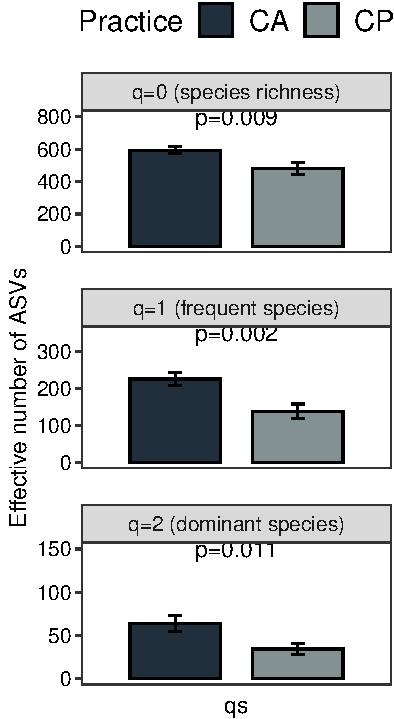
\includegraphics{Doc_pdf_files/figure-latex/unnamed-chunk-27-1} \end{center}

\begin{Shaded}
\begin{Highlighting}[]
\CommentTok{\#boxplot}
\NormalTok{boxplot\_practice\_f}\OtherTok{\textless{}{-}}\NormalTok{func }\SpecialCharTok{\%\textgreater{}\%} 
  \FunctionTok{ggbarplot}\NormalTok{(}\AttributeTok{x=}\StringTok{"fs"}\NormalTok{, }\AttributeTok{y=}\StringTok{"value"}\NormalTok{, }\AttributeTok{fill =} \StringTok{"Practice"}\NormalTok{, }\AttributeTok{add =} \StringTok{"mean\_se"}\NormalTok{, }
            \AttributeTok{position =} \FunctionTok{position\_dodge}\NormalTok{())}\SpecialCharTok{+}
  \FunctionTok{theme\_bw}\NormalTok{()}\SpecialCharTok{+}
  \FunctionTok{labs}\NormalTok{(}\AttributeTok{y =} \StringTok{"Mean functional diversity"}\NormalTok{)}\SpecialCharTok{+}
  \FunctionTok{facet\_wrap}\NormalTok{(}\SpecialCharTok{\textasciitilde{}}\NormalTok{fs, }\AttributeTok{scales =} \StringTok{"free"}\NormalTok{, }\AttributeTok{dir =} \StringTok{"v"}\NormalTok{)}\SpecialCharTok{+}
  \FunctionTok{theme}\NormalTok{(}\AttributeTok{panel.spacing=}\FunctionTok{unit}\NormalTok{(}\DecValTok{1}\NormalTok{,}\StringTok{"lines"}\NormalTok{),}
        \AttributeTok{strip.text.x =} \FunctionTok{element\_text}\NormalTok{(}\AttributeTok{size =} \DecValTok{10}\NormalTok{),}
        \AttributeTok{axis.text =}  \FunctionTok{element\_text}\NormalTok{(}\AttributeTok{colour =} \StringTok{"black"}\NormalTok{, }\AttributeTok{size =} \DecValTok{10}\NormalTok{),}
        \AttributeTok{axis.ticks.x=}\FunctionTok{element\_blank}\NormalTok{(), }
        \AttributeTok{legend.title =} \FunctionTok{element\_text}\NormalTok{(}\AttributeTok{size =} \DecValTok{14}\NormalTok{),}
        \AttributeTok{legend.text =} \FunctionTok{element\_text}\NormalTok{(}\AttributeTok{size=}\DecValTok{14}\NormalTok{), }
        \AttributeTok{axis.text.x =} \FunctionTok{element\_blank}\NormalTok{(),}
        \AttributeTok{panel.grid.major =} \FunctionTok{element\_blank}\NormalTok{(), }\AttributeTok{panel.grid.minor =} \FunctionTok{element\_blank}\NormalTok{(),}
        \AttributeTok{legend.direction =} \StringTok{"horizontal"}\NormalTok{ ,}
        \AttributeTok{legend.position =} \StringTok{"top"}\NormalTok{)}\SpecialCharTok{+}\FunctionTok{scale\_fill\_manual}\NormalTok{(}\AttributeTok{values =} \FunctionTok{c}\NormalTok{(}\StringTok{"\#212F3D"}\NormalTok{, }\StringTok{"\#839192"}\NormalTok{))}\SpecialCharTok{+} \FunctionTok{labs}\NormalTok{(}\AttributeTok{fill =} \StringTok{"Practice"}\NormalTok{)}

\NormalTok{boxplot\_practice\_f}\OtherTok{\textless{}{-}}\NormalTok{boxplot\_practice\_f }\SpecialCharTok{+}  \FunctionTok{geom\_text}\NormalTok{(}\AttributeTok{data =}\NormalTok{ ann\_text\_f,}\AttributeTok{label=}\NormalTok{ann\_text\_f}\SpecialCharTok{$}\NormalTok{label)}

\NormalTok{boxplot\_practice\_f}
\end{Highlighting}
\end{Shaded}

\begin{center}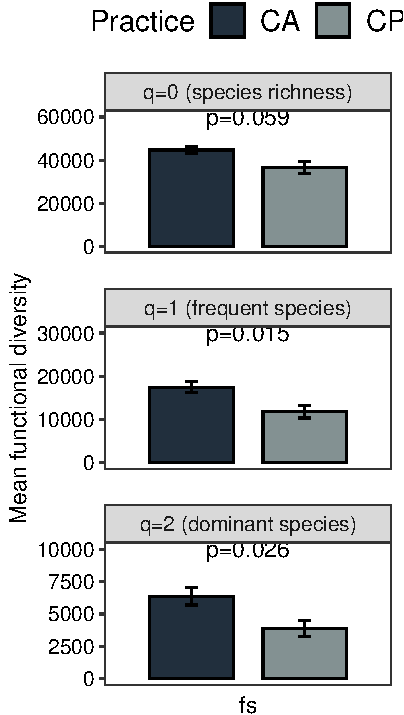
\includegraphics{Doc_pdf_files/figure-latex/unnamed-chunk-27-2} \end{center}

\begin{Shaded}
\begin{Highlighting}[]
\CommentTok{\#pdf("fig\_alpha\_practice.pdf", width=2.7, height=5)}
\CommentTok{\#print(boxplot\_practice)}
\CommentTok{\#dev.off()}
\CommentTok{\#pdf("fig\_func\_practice.pdf", width=2.7, height=5)}
\CommentTok{\#print(boxplot\_practice\_f)}
\CommentTok{\#dev.off()}
\end{Highlighting}
\end{Shaded}

\hypertarget{aldex-results-heatmap-from-soil-1}{%
\subsubsection{Aldex results heatmap from
Soil}\label{aldex-results-heatmap-from-soil-1}}

\begin{Shaded}
\begin{Highlighting}[]
\CommentTok{\#file to heatmap}
\NormalTok{aldex\_all\_dif}\OtherTok{\textless{}{-}} \FunctionTok{read\_tsv}\NormalTok{(}\StringTok{"../Data/aldex\_treatment.tsv"}\NormalTok{)}

\NormalTok{my\_fun }\OtherTok{\textless{}{-}} \ControlFlowTok{function}\NormalTok{(x) \{ }
\NormalTok{  x }\SpecialCharTok{\%\textgreater{}\%} \FunctionTok{separate}\NormalTok{(}
    \StringTok{"Taxon"}\NormalTok{, }\FunctionTok{c}\NormalTok{(}\StringTok{"k"}\NormalTok{, }\StringTok{"phylum"}\NormalTok{,}\StringTok{"c"}\NormalTok{, }\StringTok{"o"}\NormalTok{,}\StringTok{"f"}\NormalTok{,}\StringTok{"g"}\NormalTok{),}
    \AttributeTok{sep =} \StringTok{"}\SpecialCharTok{\textbackslash{}\textbackslash{}}\StringTok{;"}\NormalTok{, }\AttributeTok{remove =}\NormalTok{ F) }\SpecialCharTok{\%\textgreater{}\%}\NormalTok{ dplyr}\SpecialCharTok{::}\FunctionTok{select}\NormalTok{(}
\NormalTok{      Taxon, p.value, effect, diff.btw, rab.win}\FloatTok{.0}\NormalTok{, rab.win}\FloatTok{.1}\NormalTok{, phylum, }
      \StringTok{"FeatureID"}\OtherTok{=}\StringTok{"Feature.ID"}\NormalTok{ )}\SpecialCharTok{\%\textgreater{}\%} 
    \FunctionTok{drop\_na}\NormalTok{(.)}\SpecialCharTok{\%\textgreater{}\%} 
    \FunctionTok{rownames\_to\_column}\NormalTok{(}\AttributeTok{var=}\StringTok{"rows"}\NormalTok{)}\SpecialCharTok{\%\textgreater{}\%}       
    \FunctionTok{mutate\_all}\NormalTok{(}\FunctionTok{funs}\NormalTok{(}\FunctionTok{str\_replace}\NormalTok{(., }\StringTok{"k\_\_Bacteria;"}\NormalTok{, }\StringTok{""}\NormalTok{)))}\SpecialCharTok{\%\textgreater{}\%}
    \FunctionTok{mutate\_all}\NormalTok{(}\FunctionTok{funs}\NormalTok{(}\FunctionTok{str\_replace}\NormalTok{(., }\StringTok{"; c\_\_; o\_\_; f\_\_; g\_\_; s\_\_"}\NormalTok{, }\StringTok{""}\NormalTok{)))}\SpecialCharTok{\%\textgreater{}\%} 
    \FunctionTok{mutate\_all}\NormalTok{(}\FunctionTok{funs}\NormalTok{(}\FunctionTok{str\_replace}\NormalTok{(., }\StringTok{"; o\_\_; f\_\_; g\_\_; s\_\_"}\NormalTok{, }\StringTok{""}\NormalTok{)))}\SpecialCharTok{\%\textgreater{}\%} 
    \FunctionTok{mutate\_all}\NormalTok{(}\FunctionTok{funs}\NormalTok{(}\FunctionTok{str\_replace}\NormalTok{(., }\StringTok{"; f\_\_; g\_\_; s\_\_"}\NormalTok{, }\StringTok{""}\NormalTok{)))}\SpecialCharTok{\%\textgreater{}\%}
    \FunctionTok{mutate\_all}\NormalTok{(}\FunctionTok{funs}\NormalTok{(}\FunctionTok{str\_replace}\NormalTok{(., }\StringTok{"; g\_\_; s\_\_"}\NormalTok{, }\StringTok{""}\NormalTok{)))}\SpecialCharTok{\%\textgreater{}\%}
    \FunctionTok{mutate\_all}\NormalTok{(}\FunctionTok{funs}\NormalTok{(}\FunctionTok{str\_replace}\NormalTok{(., }\StringTok{"; s\_\_"}\NormalTok{, }\StringTok{""}\NormalTok{)))}\SpecialCharTok{\%\textgreater{}\%}\FunctionTok{mutate}\NormalTok{(}
      \AttributeTok{tax=} \FunctionTok{str\_extract}\NormalTok{(Taxon, }\StringTok{"[\^{}\_]+$"}\NormalTok{)) }\SpecialCharTok{\%\textgreater{}\%}\FunctionTok{mutate}\NormalTok{(}
        \AttributeTok{taxo =} \FunctionTok{paste}\NormalTok{(rows,}\StringTok{"\_"}\NormalTok{,tax))}\SpecialCharTok{\%\textgreater{}\%} \FunctionTok{mutate\_at}\NormalTok{(}
          \FunctionTok{c}\NormalTok{(}\DecValTok{3}\SpecialCharTok{:}\DecValTok{7}\NormalTok{), as.numeric) }\SpecialCharTok{\%\textgreater{}\%}
    \FunctionTok{mutate\_at}\NormalTok{(}\FunctionTok{c}\NormalTok{(}\DecValTok{3}\NormalTok{), }\FunctionTok{funs}\NormalTok{(}\AttributeTok{p.Value =} \FunctionTok{case\_when}\NormalTok{(}
\NormalTok{      . }\SpecialCharTok{\textless{}=} \FloatTok{0.001} \SpecialCharTok{\textasciitilde{}} \StringTok{"\textless{}0.001"}\NormalTok{,}
\NormalTok{      . }\SpecialCharTok{\textgreater{}}  \FloatTok{0.001} \SpecialCharTok{\&}\NormalTok{ .  }\SpecialCharTok{\textless{}=} \FloatTok{0.01} \SpecialCharTok{\textasciitilde{}} \StringTok{"\textless{}0.01"}\NormalTok{,}
\NormalTok{      . }\SpecialCharTok{\textgreater{}}  \FloatTok{0.01} \SpecialCharTok{\&}\NormalTok{ .  }\SpecialCharTok{\textless{}=} \FloatTok{0.05} \SpecialCharTok{\textasciitilde{}} \StringTok{"\textless{}0.05"}\NormalTok{)))}\SpecialCharTok{\%\textgreater{}\%}
    \FunctionTok{arrange}\NormalTok{(diff.btw)}\SpecialCharTok{\%\textgreater{}\%}\FunctionTok{column\_to\_rownames}\NormalTok{(}
      \AttributeTok{var =} \StringTok{"taxo"}\NormalTok{)}\SpecialCharTok{\%\textgreater{}\%} \FunctionTok{mutate\_at}\NormalTok{(}\FunctionTok{c}\NormalTok{(}\DecValTok{8}\NormalTok{),}\FunctionTok{funs}\NormalTok{(}\FunctionTok{str\_replace}\NormalTok{(., }\StringTok{"p\_\_"}\NormalTok{, }\StringTok{""}\NormalTok{)))}
\NormalTok{\}}
\CommentTok{\#We are going to multiplicate for {-}1 in order to change }
\CommentTok{\#the direction of the figure (e.g, bulk soil first and then rhizosphere)}

\NormalTok{annotation\_heatmap }\OtherTok{\textless{}{-}} \FunctionTok{my\_fun}\NormalTok{(aldex\_all\_dif) }\SpecialCharTok{\%\textgreater{}\%} 
  \FunctionTok{rename}\NormalTok{(}\AttributeTok{rab.win.CA =}\NormalTok{ rab.win}\FloatTok{.0}\NormalTok{, }\AttributeTok{rab.win.CP =}\NormalTok{ rab.win}\FloatTok{.1}\NormalTok{) }\SpecialCharTok{\%\textgreater{}\%} 
  \FunctionTok{mutate}\NormalTok{(}\AttributeTok{taxo=} \FunctionTok{paste}\NormalTok{(rows,tax, }\AttributeTok{sep =} \StringTok{"\_"}\NormalTok{))}
\NormalTok{data\_heatmap}\OtherTok{\textless{}{-}}\NormalTok{ annotation\_heatmap}\SpecialCharTok{\%\textgreater{}\%}\NormalTok{dplyr}\SpecialCharTok{::}\FunctionTok{select}\NormalTok{(rab.win.CA, rab.win.CP)}

\NormalTok{color\_heatmap}\OtherTok{=} \FunctionTok{colorRamp2}\NormalTok{(}\FunctionTok{seq}\NormalTok{(}\FunctionTok{min}\NormalTok{(data\_heatmap), }\FunctionTok{max}\NormalTok{(data\_heatmap), }\AttributeTok{length =} \DecValTok{5}\NormalTok{), }
                          \FunctionTok{c}\NormalTok{(}\StringTok{"\#0000FF"}\NormalTok{,}\StringTok{"\#5499C7"}\NormalTok{, }\StringTok{"\#DAE7E4"}\NormalTok{,  }\StringTok{"red"}\NormalTok{, }\StringTok{"\#FF0000"}\NormalTok{))}


\CommentTok{\#Annotation Phylum}
\NormalTok{cols\_ann }\OtherTok{\textless{}{-}} \FunctionTok{list}\NormalTok{(}\StringTok{\textquotesingle{}phylum\textquotesingle{}} \OtherTok{=} \FunctionTok{c}\NormalTok{(}
  \StringTok{" Acidobacteria"} \OtherTok{=} \StringTok{\textquotesingle{}red2\textquotesingle{}}\NormalTok{,}
  \StringTok{" Actinobacteria"} \OtherTok{=} \StringTok{\textquotesingle{}royalblue\textquotesingle{}}\NormalTok{,}
  \StringTok{" Bacteroidetes"}\OtherTok{=}\StringTok{"yellow"}\NormalTok{,}
  \StringTok{" Chloroflexi"} \OtherTok{=}\StringTok{"pink"}\NormalTok{,}
  \StringTok{" Firmicutes"}\OtherTok{=} \StringTok{"green"}\NormalTok{,}
  \StringTok{" Gemmatimonadetes"} \OtherTok{=} \StringTok{"black"}\NormalTok{,}
  \StringTok{" Nitrospirae"} \OtherTok{=}\StringTok{"purple"}\NormalTok{,}
  \StringTok{" Planctomycetes"} \OtherTok{=}\StringTok{"dark green"}\NormalTok{,}
  \StringTok{" Proteobacteria"}  \OtherTok{=}\StringTok{"gray"}\NormalTok{,}
  \StringTok{" Verrucomicrobia"} \OtherTok{=}\StringTok{"brown"}\NormalTok{))}
\NormalTok{colAnn }\OtherTok{\textless{}{-}} \FunctionTok{HeatmapAnnotation}\NormalTok{(}\AttributeTok{phylum =}\NormalTok{ annotation\_heatmap}\SpecialCharTok{$}\NormalTok{phylum,}
                            \AttributeTok{which =} \StringTok{\textquotesingle{}row\textquotesingle{}}\NormalTok{,}
                            \AttributeTok{col =}\NormalTok{ cols\_ann,}
                            \AttributeTok{show\_legend =}\NormalTok{ T)}

\NormalTok{cols\_pvalue }\OtherTok{\textless{}{-}} \FunctionTok{list}\NormalTok{(}\StringTok{\textquotesingle{}p{-}value\textquotesingle{}} \OtherTok{=} \FunctionTok{c}\NormalTok{(}\StringTok{"\textless{}0.001"} \OtherTok{=} \StringTok{\textquotesingle{}\#AB0000\textquotesingle{}}\NormalTok{,}
                                  \StringTok{"\textless{}0.01"} \OtherTok{=} \StringTok{\textquotesingle{}\#FF0000\textquotesingle{}}\NormalTok{,}
                                  \StringTok{"\textless{}0.05"}\OtherTok{=}\StringTok{"\#FFB6B6"}\NormalTok{))}

\NormalTok{annP2 }\OtherTok{=} \FunctionTok{HeatmapAnnotation}\NormalTok{(}\StringTok{"p{-}value"} \OtherTok{=}\NormalTok{ annotation\_heatmap}\SpecialCharTok{$}\NormalTok{p.Value,}
                          \AttributeTok{which =} \StringTok{"row"}\NormalTok{, }\AttributeTok{col =}\NormalTok{ cols\_pvalue,}
                          \AttributeTok{show\_legend =}\NormalTok{ T)}\CommentTok{\#, gp = gpar(col = "white"))}


\CommentTok{\#Annotation effect size}
\NormalTok{effect\_col\_fun }\OtherTok{=}\FunctionTok{colorRamp2}\NormalTok{(}\FunctionTok{c}\NormalTok{(}\SpecialCharTok{{-}}\FloatTok{1.5}\NormalTok{, }\DecValTok{0}\NormalTok{, }\FloatTok{1.5}\NormalTok{), }\FunctionTok{c}\NormalTok{(}\StringTok{"lightsalmon4"}\NormalTok{, }\StringTok{"white"}\NormalTok{, }\StringTok{"lightseagreen"}\NormalTok{))}

\NormalTok{annEffect }\OtherTok{=} \FunctionTok{HeatmapAnnotation}\NormalTok{(}\StringTok{"effect{-}size"} \OtherTok{=}\NormalTok{ annotation\_heatmap}\SpecialCharTok{$}\NormalTok{effect,}
                              \AttributeTok{which =} \StringTok{"row"}\NormalTok{, }\AttributeTok{col =} \FunctionTok{list}\NormalTok{(}\StringTok{"effect{-}size"} \OtherTok{=}\NormalTok{ effect\_col\_fun),}
                              \AttributeTok{show\_legend =}\NormalTok{ T, }
                              \AttributeTok{gp =} \FunctionTok{gpar}\NormalTok{(}\AttributeTok{col =} \StringTok{"white"}\NormalTok{))}

\CommentTok{\#Annotation barplot}
\NormalTok{bardif}\OtherTok{=} \FunctionTok{rowAnnotation}\NormalTok{(}\StringTok{"difference }\SpecialCharTok{\textbackslash{}n}\StringTok{ between groups"} \OtherTok{=} \FunctionTok{anno\_barplot}\NormalTok{(}
\NormalTok{  annotation\_heatmap}\SpecialCharTok{$}\NormalTok{diff.btw, }\AttributeTok{width =} \FunctionTok{unit}\NormalTok{(}\DecValTok{4}\NormalTok{, }\StringTok{"cm"}\NormalTok{)))}


\CommentTok{\#Annotation taxonomy}

\NormalTok{labels }\OtherTok{=} \FunctionTok{c}\NormalTok{(}\StringTok{"Ellin6075"}\NormalTok{, }\StringTok{"SC{-}I{-}84"}\NormalTok{, }\StringTok{""}\NormalTok{, }\StringTok{"iii1{-}15"}\NormalTok{ ,  }\StringTok{"Gemm{-}1"}\NormalTok{,}\StringTok{""}\NormalTok{, }
\StringTok{"Rhizobiales"}\NormalTok{ , }\StringTok{"Ellin5301"}\NormalTok{,  }\StringTok{"Xanthomonadaceae"}\NormalTok{  , }
\StringTok{"Cytophagaceae"}\NormalTok{ ,}\StringTok{"iii1{-}15"}\NormalTok{, }\StringTok{""}\NormalTok{ ,}\StringTok{"Flavisolibacter"}\NormalTok{ , }\StringTok{"iii1{-}15"}\NormalTok{, }\StringTok{"Chitinophagaceae"}\NormalTok{,}
\StringTok{"Acidobacteria{-}6"}\NormalTok{,  }\StringTok{"Chitinophagaceae"}\NormalTok{, }\StringTok{"iii1{-}15"}\NormalTok{ , }\StringTok{"iii1{-}15"}\NormalTok{, }\StringTok{"OR{-}59"}\NormalTok{, }\StringTok{"Ellin6075"}\NormalTok{, }
\StringTok{"Microbacteriaceae"}\NormalTok{,}\StringTok{"Nitrospira"}\NormalTok{ ,}\StringTok{"Chitinophagaceae"}\NormalTok{,}\StringTok{"Ellin5290"}\NormalTok{,  }\StringTok{""}\NormalTok{,}\StringTok{"Ellin6529"}\NormalTok{ ,}
\StringTok{"Flavobacterium"}\NormalTok{  , }\StringTok{"Cytophagaceae"}\NormalTok{, }\StringTok{"Chitinophagaceae"}\NormalTok{,}\StringTok{"Xanthomonadaceae"}\NormalTok{ ,}\StringTok{"Chitinophagaceae"}\NormalTok{, }
\StringTok{"OR{-}59"}\NormalTok{,  }\StringTok{"Chitinophagaceae"}\NormalTok{  ,  }\StringTok{"Chitinophagaceae"}\NormalTok{ ,}\StringTok{"mb2424"}\NormalTok{, }
\StringTok{"Xanthomonadaceae"}\NormalTok{, }\StringTok{"Chitinophagaceae"}\NormalTok{  ,  }\StringTok{"iii1{-}15"}\NormalTok{,}\StringTok{"Chitinophagaceae"}\NormalTok{ ,}\StringTok{""}\NormalTok{  , }\StringTok{"Xanthomonadaceae"}\NormalTok{,}
\StringTok{"[Chthoniobacteraceae]"}\NormalTok{,  }\StringTok{"C111"}\NormalTok{  ,  }\StringTok{"iii1{-}15"}\NormalTok{  , }\StringTok{"Flavisolibacter"}\NormalTok{,  }\StringTok{""}\NormalTok{,  }\StringTok{"[Chthoniobacteraceae]"}\NormalTok{ ,}
\StringTok{""}\NormalTok{, }\StringTok{""}\NormalTok{ ,}\StringTok{"Micromonosporaceae"}\NormalTok{ , }\StringTok{"Rhizobiales"}\NormalTok{  , }\StringTok{"WD2101"}\NormalTok{ , }\StringTok{"iii1{-}15"}\NormalTok{ ,  }
\StringTok{"Flavobacterium"}\NormalTok{, }\FunctionTok{rep}\NormalTok{(}\StringTok{""}\NormalTok{, }\DecValTok{11}\NormalTok{), }\StringTok{"Roseococcus"}\NormalTok{  , }\StringTok{"Comamonadaceae"}\NormalTok{ ,  }\StringTok{"Chitinophagaceae"}\NormalTok{ ,  }
\StringTok{"Chitinophagaceae"}\NormalTok{ ,}\StringTok{"DA{-}101"}\NormalTok{ ,  }\StringTok{""}\NormalTok{, }\StringTok{"WD2101"}\NormalTok{ , }\StringTok{""}\NormalTok{  ,}\StringTok{"WD2101"}\NormalTok{, }
\StringTok{"Oxalobacteraceae"}\NormalTok{, }\StringTok{"Ellin5301"}\NormalTok{,  }\StringTok{"iii1{-}15"}\NormalTok{,}\StringTok{"iii1{-}15"}\NormalTok{ ,}\StringTok{"Ellin5290"}\NormalTok{ , }\StringTok{""}\NormalTok{ ,}
\StringTok{""}\NormalTok{ , }\StringTok{""}\NormalTok{, }\StringTok{"Flavisolibacter"}\NormalTok{,}\StringTok{"Oxalobacteraceae"}\NormalTok{, }\StringTok{"RB41"}\NormalTok{,}\StringTok{"iii1{-}15"}\NormalTok{) }

\NormalTok{heatmap\_aldex\_treatment}\OtherTok{\textless{}{-}}\NormalTok{ComplexHeatmap}\SpecialCharTok{::}  \FunctionTok{Heatmap}\NormalTok{(data\_heatmap, }\AttributeTok{col =}\NormalTok{ color\_heatmap, }\AttributeTok{row\_dend\_reorder =}\NormalTok{ F, }\AttributeTok{width =} \FunctionTok{ncol}\NormalTok{(data\_heatmap)}\SpecialCharTok{*}\FunctionTok{unit}\NormalTok{(}\DecValTok{1}\NormalTok{, }\StringTok{"cm"}\NormalTok{),}
\AttributeTok{height =} \FunctionTok{ncol}\NormalTok{(data\_heatmap)}\SpecialCharTok{*}\FunctionTok{unit}\NormalTok{(}\DecValTok{8}\NormalTok{, }\StringTok{"cm"}\NormalTok{),}
\AttributeTok{left\_annotation =}  \FunctionTok{c}\NormalTok{(annP2, annEffect, colAnn),}
\AttributeTok{cluster\_column\_slices =}\NormalTok{ F,}
 \AttributeTok{heatmap\_legend\_param =} \FunctionTok{list}\NormalTok{(}\AttributeTok{direction =} \StringTok{"horizontal"}\NormalTok{ ),}
\AttributeTok{right\_annotation =} \FunctionTok{c}\NormalTok{(bardif),}
\AttributeTok{column\_split =} \FunctionTok{rep}\NormalTok{(}\FunctionTok{c}\NormalTok{(}\StringTok{"CA"}\NormalTok{, }\StringTok{"CP"}\NormalTok{)),}
\AttributeTok{cluster\_rows =}\NormalTok{ F,}
\AttributeTok{cluster\_columns =}\NormalTok{ F,}
\AttributeTok{column\_km =} \DecValTok{1}\NormalTok{, }\AttributeTok{column\_title\_gp =} \FunctionTok{gpar}\NormalTok{(}
\AttributeTok{fill =} \FunctionTok{c}\NormalTok{(}\StringTok{"\#212F3D"}\NormalTok{, }\StringTok{"\#839192"}\NormalTok{ ), }\AttributeTok{col=}\StringTok{"white"}\NormalTok{),}
\AttributeTok{border =}\NormalTok{ F, }\AttributeTok{column\_gap =} \FunctionTok{unit}\NormalTok{(}\FloatTok{0.5}\NormalTok{, }\StringTok{"mm"}\NormalTok{), }
\AttributeTok{row\_dend\_side =} \StringTok{"left"}\NormalTok{,}\AttributeTok{row\_names\_side =} \StringTok{"right"}\NormalTok{,}
\AttributeTok{show\_row\_names =}\NormalTok{ F ,}\AttributeTok{rect\_gp =} \FunctionTok{gpar}\NormalTok{(}\AttributeTok{col =} \StringTok{"white"}\NormalTok{, }\AttributeTok{lwd =} \FloatTok{0.2}\NormalTok{), }
\AttributeTok{row\_names\_gp =} \FunctionTok{gpar}\NormalTok{(}\AttributeTok{fontface =}\StringTok{"italic"}\NormalTok{, }\AttributeTok{fontsize=}\DecValTok{10}\NormalTok{),}
\AttributeTok{show\_column\_names =}\NormalTok{ F, }\AttributeTok{name =} \StringTok{"rab.Win"}\NormalTok{) }\SpecialCharTok{+} 
\FunctionTok{rowAnnotation}\NormalTok{(}\AttributeTok{labels =} \FunctionTok{anno\_text}\NormalTok{(labels, }\AttributeTok{which =} \StringTok{"row"}\NormalTok{, }\FunctionTok{gpar}\NormalTok{(}
  \AttributeTok{col =} \StringTok{"black"}\NormalTok{, }\AttributeTok{fontsize =} \DecValTok{6}\NormalTok{)), }\AttributeTok{width =} \FunctionTok{unit}\NormalTok{(}\DecValTok{2}\NormalTok{, }\StringTok{"cm"}\NormalTok{))}

\NormalTok{heatmap\_aldex\_treatment}
\end{Highlighting}
\end{Shaded}

\begin{center}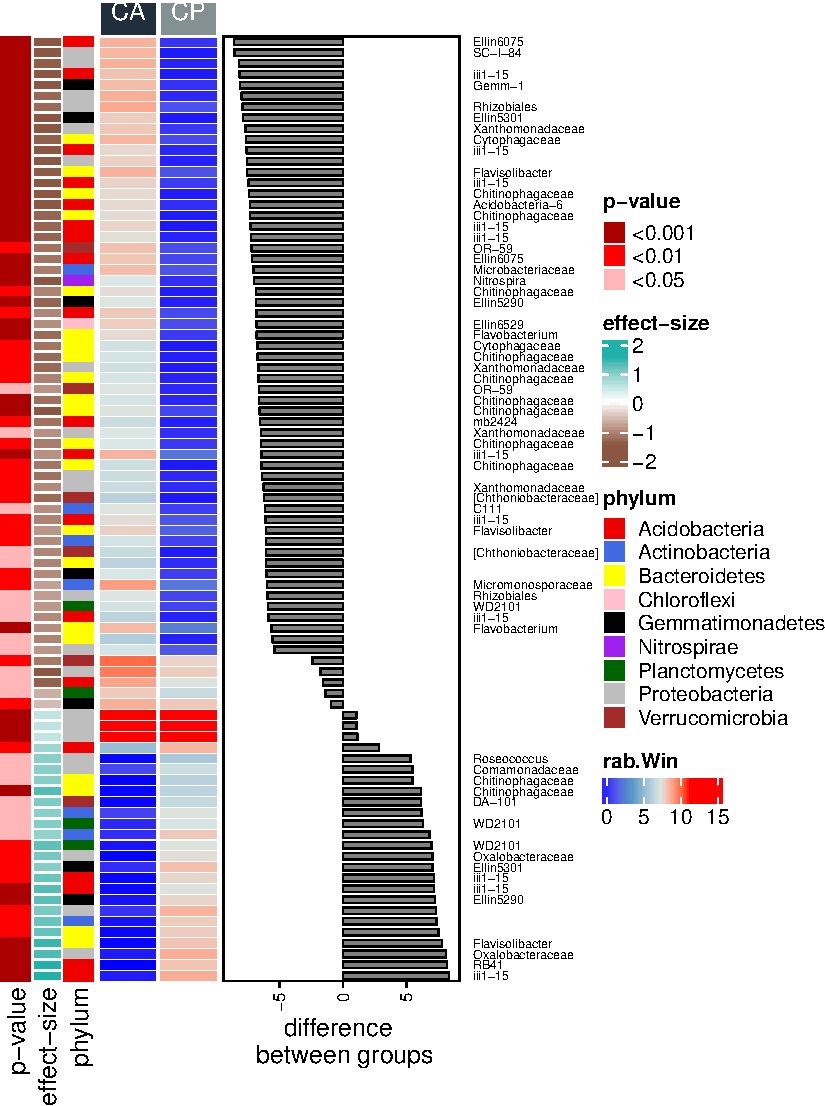
\includegraphics{Doc_pdf_files/figure-latex/unnamed-chunk-28-1} \end{center}

\begin{Shaded}
\begin{Highlighting}[]
\CommentTok{\#pdf("fig\_aldex\_TREATMENT.pdf", width=6, height=8)}
\CommentTok{\#print(heatmap\_aldex\_treatment)}
\CommentTok{\#dev.off()}
\end{Highlighting}
\end{Shaded}

\hypertarget{pca-plot-1}{%
\subsubsection{PCA plot}\label{pca-plot-1}}

\begin{Shaded}
\begin{Highlighting}[]
\CommentTok{\#loading files and formatting}

\NormalTok{d.pro}\FloatTok{.0}\OtherTok{\textless{}{-}} \FunctionTok{read\_tsv}\NormalTok{(}\StringTok{"../Data/otutable.tsv"}\NormalTok{)}\SpecialCharTok{\%\textgreater{}\%} \FunctionTok{column\_to\_rownames}\NormalTok{(}\AttributeTok{var =} \StringTok{"\#OTU ID"}\NormalTok{)}
\NormalTok{meta}\OtherTok{\textless{}{-}}\FunctionTok{read\_tsv}\NormalTok{(}\StringTok{"../Data/metadata.tsv"}\NormalTok{)}

\NormalTok{meta}\SpecialCharTok{$}\NormalTok{Treatment}\OtherTok{\textless{}{-}} \FunctionTok{factor}\NormalTok{(meta}\SpecialCharTok{$}\NormalTok{Treatment,}
                       \AttributeTok{levels =} \FunctionTok{c}\NormalTok{( }\StringTok{"AC"}\NormalTok{, }\StringTok{"AT"}\NormalTok{),}
                       \AttributeTok{labels =} \FunctionTok{c}\NormalTok{(}\StringTok{"CA"}\NormalTok{, }\StringTok{"CP"}\NormalTok{))}

\NormalTok{tax}\OtherTok{\textless{}{-}}\FunctionTok{read\_tsv}\NormalTok{(}\StringTok{"../Data/taxonomy.tsv"}\NormalTok{) }\SpecialCharTok{\%\textgreater{}\%}\NormalTok{ dplyr}\SpecialCharTok{::}\FunctionTok{select}\NormalTok{(}\SpecialCharTok{{-}}\NormalTok{Confidence)}\SpecialCharTok{\%\textgreater{}\%}
  \FunctionTok{mutate\_all}\NormalTok{(}\FunctionTok{funs}\NormalTok{(}\FunctionTok{str\_replace}\NormalTok{(., }\StringTok{"k\_\_Bacteria;"}\NormalTok{, }\StringTok{""}\NormalTok{)))}\SpecialCharTok{\%\textgreater{}\%} 
  \FunctionTok{mutate\_all}\NormalTok{(}\FunctionTok{funs}\NormalTok{(}\FunctionTok{str\_replace}\NormalTok{(., }\StringTok{"p\_\_"}\NormalTok{, }\StringTok{""}\NormalTok{)))}\SpecialCharTok{\%\textgreater{}\%} 
  \FunctionTok{mutate\_all}\NormalTok{(}\FunctionTok{funs}\NormalTok{(}\FunctionTok{str\_replace}\NormalTok{(., }\StringTok{"c\_\_"}\NormalTok{, }\StringTok{""}\NormalTok{)))}\SpecialCharTok{\%\textgreater{}\%} 
  \FunctionTok{mutate\_all}\NormalTok{(}\FunctionTok{funs}\NormalTok{(}\FunctionTok{str\_replace}\NormalTok{(., }\StringTok{"o\_\_"}\NormalTok{, }\StringTok{""}\NormalTok{)))}\SpecialCharTok{\%\textgreater{}\%} 
  \FunctionTok{mutate\_all}\NormalTok{(}\FunctionTok{funs}\NormalTok{(}\FunctionTok{str\_replace}\NormalTok{(., }\StringTok{"f\_\_"}\NormalTok{, }\StringTok{""}\NormalTok{)))}\SpecialCharTok{\%\textgreater{}\%} 
  \FunctionTok{mutate\_all}\NormalTok{(}\FunctionTok{funs}\NormalTok{(}\FunctionTok{str\_replace}\NormalTok{(., }\StringTok{"g\_\_"}\NormalTok{, }\StringTok{""}\NormalTok{)))}\SpecialCharTok{\%\textgreater{}\%} 
  \FunctionTok{mutate\_all}\NormalTok{(}\FunctionTok{funs}\NormalTok{(}\FunctionTok{str\_replace}\NormalTok{(., }\StringTok{"s\_\_"}\NormalTok{, }\StringTok{""}\NormalTok{)))}\SpecialCharTok{\%\textgreater{}\%} 
  \FunctionTok{mutate\_all}\NormalTok{(}\FunctionTok{funs}\NormalTok{(}\FunctionTok{str\_replace}\NormalTok{(., }\StringTok{"; ; ;"}\NormalTok{, }\StringTok{""}\NormalTok{)))}\SpecialCharTok{\%\textgreater{}\%} 
  \FunctionTok{mutate\_all}\NormalTok{(}\FunctionTok{funs}\NormalTok{(}\FunctionTok{str\_replace}\NormalTok{(., }\StringTok{"; ; "}\NormalTok{, }\StringTok{""}\NormalTok{))) }\SpecialCharTok{\%\textgreater{}\%} \FunctionTok{rename}\NormalTok{(}
    \StringTok{"FeatureID"}\OtherTok{=}\StringTok{\textasciigrave{}}\AttributeTok{\#OTU ID}\StringTok{\textasciigrave{}}\NormalTok{, }\AttributeTok{Taxon=}\NormalTok{ taxonomy)}

\NormalTok{tax2}\OtherTok{\textless{}{-}} \FunctionTok{read\_tsv}\NormalTok{(}\StringTok{"../Data/taxonomy.tsv"}\NormalTok{) }\SpecialCharTok{\%\textgreater{}\%}\NormalTok{ dplyr}\SpecialCharTok{::}\FunctionTok{select}\NormalTok{(}
  \SpecialCharTok{{-}}\NormalTok{Confidence) }\SpecialCharTok{\%\textgreater{}\%} \FunctionTok{rename}\NormalTok{(}
    \StringTok{"FeatureID"}\OtherTok{=}\StringTok{\textasciigrave{}}\AttributeTok{\#OTU ID}\StringTok{\textasciigrave{}}\NormalTok{, }\AttributeTok{Taxon=}\NormalTok{ taxonomy)}


\CommentTok{\#transforming data}
\NormalTok{d.pro }\OtherTok{\textless{}{-}} \FunctionTok{cmultRepl}\NormalTok{(}\FunctionTok{t}\NormalTok{(d.pro}\FloatTok{.0}\NormalTok{), }\AttributeTok{method=}\StringTok{"CZM"}\NormalTok{, }\AttributeTok{output=}\StringTok{"p{-}counts"}\NormalTok{)}
\NormalTok{d.clr.abund.codaseq}\OtherTok{\textless{}{-}}\FunctionTok{codaSeq.clr}\NormalTok{(}\AttributeTok{x =}\NormalTok{ d.pro,}\AttributeTok{samples.by.row =}\NormalTok{ F)}

\CommentTok{\#run pca}
\NormalTok{pcx.abund }\OtherTok{\textless{}{-}} \FunctionTok{prcomp}\NormalTok{(d.clr.abund.codaseq)}

\CommentTok{\#labels to pca axis}

\NormalTok{PC1 }\OtherTok{\textless{}{-}} \FunctionTok{paste}\NormalTok{(}\StringTok{"PC1"}\NormalTok{, }\FunctionTok{round}\NormalTok{(}\FunctionTok{sum}\NormalTok{(pcx.abund}\SpecialCharTok{$}\NormalTok{sdev[}\DecValTok{1}\NormalTok{] }\SpecialCharTok{\^{}} \DecValTok{2}\NormalTok{) }\SpecialCharTok{/} \FunctionTok{mvar}\NormalTok{(d.clr.abund.codaseq) }\SpecialCharTok{*} \DecValTok{100}\NormalTok{, }\DecValTok{1}\NormalTok{), }\StringTok{"\%"}\NormalTok{)}
\NormalTok{PC2 }\OtherTok{\textless{}{-}} \FunctionTok{paste}\NormalTok{(}\StringTok{"P21"}\NormalTok{, }\FunctionTok{round}\NormalTok{(}\FunctionTok{sum}\NormalTok{(pcx.abund}\SpecialCharTok{$}\NormalTok{sdev[}\DecValTok{2}\NormalTok{] }\SpecialCharTok{\^{}} \DecValTok{2}\NormalTok{) }\SpecialCharTok{/} \FunctionTok{mvar}\NormalTok{(d.clr.abund.codaseq) }\SpecialCharTok{*} \DecValTok{100}\NormalTok{, }\DecValTok{1}\NormalTok{), }\StringTok{"\%"}\NormalTok{)}


\CommentTok{\#let\textquotesingle{}s choose som of the significant groups from aldex analysis }

\NormalTok{vars\_chosen}\OtherTok{\textless{}{-}} \FunctionTok{c}\NormalTok{(}\StringTok{"52\_Flavisolibacter"}\NormalTok{, }
                \StringTok{"37\_OR{-}59"}\NormalTok{,}
                \StringTok{"47\_Nitrospira"}\NormalTok{ , }
                \StringTok{"16\_Halomonas"}\NormalTok{, }
                \StringTok{"29\_Flavobacterium"}\NormalTok{,}
                \StringTok{"   27\_Steroidobacter"}\NormalTok{ , }
                \StringTok{"36\_Roseococcus"}\NormalTok{) }
\CommentTok{\#these ones were chosen from before (some aldex significant groups)}
\CommentTok{\#these ones were chosen from before (some aldex significant groups)}

\NormalTok{vars\_to\_choose}\OtherTok{\textless{}{-}}\NormalTok{ annotation\_heatmap }\SpecialCharTok{\%\textgreater{}\%}  \FunctionTok{filter}\NormalTok{(taxo }\SpecialCharTok{\%in\%}\NormalTok{ vars\_chosen)}

\NormalTok{vars\_choosing}\OtherTok{\textless{}{-}} \FunctionTok{data.frame}\NormalTok{(pcx.abund}\SpecialCharTok{$}\NormalTok{rotation) }\SpecialCharTok{\%\textgreater{}\%}  \FunctionTok{rownames\_to\_column}\NormalTok{(}\AttributeTok{var =} \StringTok{"FeatureID"}\NormalTok{)}\SpecialCharTok{\%\textgreater{}\%}   
  \FunctionTok{mutate}\NormalTok{(}\AttributeTok{a=}\FunctionTok{sqrt}\NormalTok{(PC1}\SpecialCharTok{\^{}}\DecValTok{2}\SpecialCharTok{+}\NormalTok{PC2}\SpecialCharTok{\^{}}\DecValTok{2}\NormalTok{)) }\SpecialCharTok{\%\textgreater{}\%}
  \FunctionTok{mutate}\NormalTok{(}\AttributeTok{PC1=}\NormalTok{PC1}\SpecialCharTok{*}\DecValTok{500}\NormalTok{, }\AttributeTok{PC2=}\NormalTok{PC2}\SpecialCharTok{*}\DecValTok{500}\NormalTok{) }\SpecialCharTok{\%\textgreater{}\%} \FunctionTok{left\_join}\NormalTok{(tax2)}\SpecialCharTok{\%\textgreater{}\%}\NormalTok{ dplyr}\SpecialCharTok{::}\FunctionTok{select}\NormalTok{(}
\NormalTok{    Taxon, PC1, PC2, FeatureID)}\SpecialCharTok{\%\textgreater{}\%}\FunctionTok{right\_join}\NormalTok{(vars\_to\_choose, }\AttributeTok{by =} \StringTok{"FeatureID"}\NormalTok{)}

\CommentTok{\#pca plot}
\NormalTok{pca\_treatment\_arrows}\OtherTok{\textless{}{-}} \FunctionTok{ggplot}\NormalTok{() }\SpecialCharTok{+}
  \FunctionTok{theme\_bw}\NormalTok{() }\SpecialCharTok{+}
  \FunctionTok{xlab}\NormalTok{(PC1) }\SpecialCharTok{+}
  \FunctionTok{ylab}\NormalTok{(PC2) }\SpecialCharTok{+}
  \FunctionTok{theme}\NormalTok{(}\AttributeTok{axis.text =} \FunctionTok{element\_text}\NormalTok{(}\AttributeTok{colour =} \StringTok{"black"}\NormalTok{, }\AttributeTok{size =} \DecValTok{14}\NormalTok{),}\CommentTok{\#setiing theme}
        \AttributeTok{axis.title =} \FunctionTok{element\_text}\NormalTok{(}\AttributeTok{colour =} \StringTok{"black"}\NormalTok{, }\AttributeTok{size =} \DecValTok{14}\NormalTok{),}
        \AttributeTok{legend.text =} \FunctionTok{element\_text}\NormalTok{(}\AttributeTok{size =} \DecValTok{14}\NormalTok{),}
        \AttributeTok{legend.title =} \FunctionTok{element\_blank}\NormalTok{(), }
        \AttributeTok{legend.position =} \StringTok{"bottom"}\NormalTok{) }\SpecialCharTok{+}
  \FunctionTok{geom\_point}\NormalTok{(                              }\CommentTok{\#individuals}
    \AttributeTok{data=}\FunctionTok{data.frame}\NormalTok{(pcx.abund}\SpecialCharTok{$}\NormalTok{x) }\SpecialCharTok{\%\textgreater{}\%}   \FunctionTok{rownames\_to\_column}\NormalTok{(}\AttributeTok{var =} \StringTok{"SampleID"}\NormalTok{)}\SpecialCharTok{\%\textgreater{}\%}
      \FunctionTok{left\_join}\NormalTok{(meta, }\AttributeTok{by =} \StringTok{"SampleID"}\NormalTok{),}
    \FunctionTok{aes}\NormalTok{(}\AttributeTok{x=}\NormalTok{PC1, }\AttributeTok{y=}\NormalTok{PC2, }\AttributeTok{fill=}\NormalTok{Treatment), }
    \AttributeTok{shape=}\DecValTok{21}\NormalTok{, }\AttributeTok{size=}\DecValTok{4}\NormalTok{) }\SpecialCharTok{+} 
  \FunctionTok{geom\_vline}\NormalTok{(}\AttributeTok{xintercept =} \DecValTok{0}\NormalTok{, }\AttributeTok{linetype =} \DecValTok{2}\NormalTok{) }\SpecialCharTok{+}   \CommentTok{\#lines{-}cross}
  \FunctionTok{geom\_hline}\NormalTok{(}\AttributeTok{yintercept =} \DecValTok{0}\NormalTok{, }\AttributeTok{linetype =} \DecValTok{2}\NormalTok{) }\SpecialCharTok{+}
  \FunctionTok{scale\_fill\_manual}\NormalTok{(}\AttributeTok{values =} \FunctionTok{c}\NormalTok{(}\StringTok{"\#212F3D"}\NormalTok{,}\StringTok{"\#839192"}\NormalTok{))}\SpecialCharTok{+}
\NormalTok{  ggrepel}\SpecialCharTok{::}\FunctionTok{geom\_label\_repel}\NormalTok{(}\AttributeTok{data =}\NormalTok{ vars\_choosing, }\FunctionTok{aes}\NormalTok{(}\AttributeTok{x=}\NormalTok{PC1, }\AttributeTok{y=}\NormalTok{PC2, }\AttributeTok{label=}\NormalTok{ tax),}
                            \AttributeTok{segment.colour =} \ConstantTok{NA}\NormalTok{, }\AttributeTok{box.padding =} \DecValTok{2}\NormalTok{, }\AttributeTok{fontface=}\StringTok{"italic"}\NormalTok{)}\SpecialCharTok{+}
  \FunctionTok{geom\_segment}\NormalTok{(}\AttributeTok{data =}\NormalTok{ vars\_choosing, }\FunctionTok{aes}\NormalTok{(}\AttributeTok{x=}\DecValTok{0}\NormalTok{, }\AttributeTok{y=}\DecValTok{0}\NormalTok{, }\AttributeTok{xend=}\NormalTok{PC1, }\AttributeTok{yend=}\NormalTok{PC2), }
               \AttributeTok{arrow=}\FunctionTok{arrow}\NormalTok{(}\AttributeTok{length=}\FunctionTok{unit}\NormalTok{(}\FloatTok{0.15}\NormalTok{,}\StringTok{"cm"}\NormalTok{)),}
               \AttributeTok{size=} \FloatTok{0.6}\NormalTok{)}

\NormalTok{pca\_treatment\_arrows}
\end{Highlighting}
\end{Shaded}

\begin{center}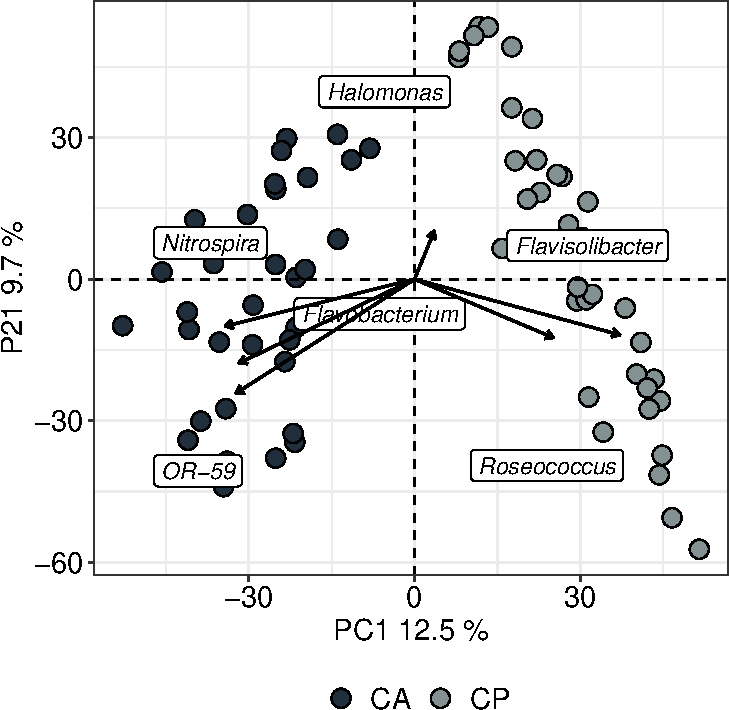
\includegraphics{Doc_pdf_files/figure-latex/unnamed-chunk-29-1} \end{center}

\begin{Shaded}
\begin{Highlighting}[]
\CommentTok{\#pdf("fig\_pca\_treatment.pdf", width=5, height=5)}
\CommentTok{\#print(pca\_treatment\_arrows)}
\CommentTok{\#dev.off()}
\end{Highlighting}
\end{Shaded}

\hypertarget{vi.-stage-figure}{%
\section{VI. STAGE FIGURE}\label{vi.-stage-figure}}

\hypertarget{loading-libraries-4}{%
\subsubsection{Loading libraries}\label{loading-libraries-4}}

\begin{Shaded}
\begin{Highlighting}[]
\FunctionTok{library}\NormalTok{(cowplot)}
\FunctionTok{library}\NormalTok{(tidyverse)}
\FunctionTok{library}\NormalTok{(ggpubr)}
\FunctionTok{library}\NormalTok{(ComplexHeatmap)}
\FunctionTok{library}\NormalTok{(circlize)}
\FunctionTok{library}\NormalTok{(viridis)}
\FunctionTok{library}\NormalTok{(RColorBrewer)}
\FunctionTok{library}\NormalTok{(grid)}
\FunctionTok{library}\NormalTok{(CoDaSeq)}
\FunctionTok{library}\NormalTok{(ggplot2)}
\FunctionTok{require}\NormalTok{(compositions) }\CommentTok{\# exploratory d ata analysis of compositional data}
\FunctionTok{require}\NormalTok{(zCompositions) }\CommentTok{\# used for 0 substitution}
\FunctionTok{require}\NormalTok{(ALDEx2) }\CommentTok{\# used for per{-}OTU comparisons}
\FunctionTok{library}\NormalTok{(CoDaSeq)}
\FunctionTok{library}\NormalTok{(ggrepel)}
\end{Highlighting}
\end{Shaded}

\hypertarget{loadings-files-and-barplot-text-annotations-2}{%
\subsubsection{Loadings files and Barplot Text
annotations}\label{loadings-files-and-barplot-text-annotations-2}}

\begin{Shaded}
\begin{Highlighting}[]
\NormalTok{alpha}\OtherTok{\textless{}{-}} \FunctionTok{read.delim}\NormalTok{(}\StringTok{"../Data/Alpha{-}t\_asv\_table.txt"}\NormalTok{) }\SpecialCharTok{\%\textgreater{}\%} \FunctionTok{gather}\NormalTok{(}
\NormalTok{  q0}\SpecialCharTok{:}\NormalTok{q4, }\AttributeTok{key =} \StringTok{"q"}\NormalTok{, }\AttributeTok{value =} \StringTok{"value"}\NormalTok{) }\SpecialCharTok{\%\textgreater{}\%} \FunctionTok{filter}\NormalTok{(}
\NormalTok{  q }\SpecialCharTok{\%in\%} \FunctionTok{c}\NormalTok{(}\StringTok{"q0"}\NormalTok{, }\StringTok{"q1"}\NormalTok{, }\StringTok{"q2"}\NormalTok{))}\SpecialCharTok{\%\textgreater{}\%}\FunctionTok{mutate}\NormalTok{(}\AttributeTok{qs=} \FunctionTok{case\_when}\NormalTok{(}
  \FunctionTok{str\_detect}\NormalTok{(q, }\StringTok{"q0"}\NormalTok{) }\SpecialCharTok{\textasciitilde{}} \StringTok{"q0 (species richness)"}\NormalTok{,}
  \FunctionTok{str\_detect}\NormalTok{(q, }\StringTok{"q1"}\NormalTok{) }\SpecialCharTok{\textasciitilde{}} \StringTok{"q1 (frequent species)"}\NormalTok{,}
  \FunctionTok{str\_detect}\NormalTok{(q, }\StringTok{"q2"}\NormalTok{) }\SpecialCharTok{\textasciitilde{}} \StringTok{"q2 (dominant species)"}\NormalTok{))}

\NormalTok{alpha}\SpecialCharTok{$}\NormalTok{Stage }\OtherTok{\textless{}{-}} \FunctionTok{factor}\NormalTok{(alpha}\SpecialCharTok{$}\NormalTok{Stage,}
                      \AttributeTok{levels =} \FunctionTok{c}\NormalTok{(}\StringTok{\textquotesingle{}V\textquotesingle{}}\NormalTok{,}\StringTok{\textquotesingle{}F\textquotesingle{}}\NormalTok{, }\StringTok{\textquotesingle{}G\textquotesingle{}}\NormalTok{),}\AttributeTok{ordered =} \ConstantTok{TRUE}\NormalTok{)}

\NormalTok{alpha}\OtherTok{\textless{}{-}}\NormalTok{alpha}\SpecialCharTok{\%\textgreater{}\%}\FunctionTok{arrange}\NormalTok{(Stage)}

\FunctionTok{head}\NormalTok{(alpha)}
\end{Highlighting}
\end{Shaded}

\begin{verbatim}
##            X Practice Soil Practice.Location Stage Age Plant Plot ExpUnit  q
## 1 CAVBS.18.1       CA   BS             CA.BS     V   3     1   18 CA.BS.V q0
## 2 CAVBS.18.2       CA   BS             CA.BS     V   3     2   18 CA.BS.V q0
## 3 CAVBS.18.3       CA   BS             CA.BS     V   3     3   18 CA.BS.V q0
## 4 CAVBS.59.1       CA   BS             CA.BS     V   3     1   59 CA.BS.V q0
## 5 CAVBS.59.2       CA   BS             CA.BS     V   3     2   59 CA.BS.V q0
## 6 CAVBS.59.3       CA   BS             CA.BS     V   3     3   59 CA.BS.V q0
##   value                    qs
## 1   524 q0 (species richness)
## 2   711 q0 (species richness)
## 3   516 q0 (species richness)
## 4   625 q0 (species richness)
## 5   369 q0 (species richness)
## 6   530 q0 (species richness)
\end{verbatim}

\begin{Shaded}
\begin{Highlighting}[]
\NormalTok{func}\OtherTok{\textless{}{-}} \FunctionTok{read.table}\NormalTok{(}\StringTok{"../Data/func\_MDq.txt"}\NormalTok{) }\SpecialCharTok{\%\textgreater{}\%} \FunctionTok{gather}\NormalTok{(}
\NormalTok{  MD\_q0}\SpecialCharTok{:}\NormalTok{MD\_q2, }\AttributeTok{key =} \StringTok{"q"}\NormalTok{, }\AttributeTok{value =} \StringTok{"value"}\NormalTok{)}\SpecialCharTok{\%\textgreater{}\%}\FunctionTok{mutate}\NormalTok{(}\AttributeTok{fs=} \FunctionTok{case\_when}\NormalTok{(}
  \FunctionTok{str\_detect}\NormalTok{(q, }\StringTok{"q0"}\NormalTok{) }\SpecialCharTok{\textasciitilde{}} \StringTok{"q=0 (species richness)"}\NormalTok{,}
  \FunctionTok{str\_detect}\NormalTok{(q, }\StringTok{"q1"}\NormalTok{) }\SpecialCharTok{\textasciitilde{}} \StringTok{"q=1 (frequent species)"}\NormalTok{,}
  \FunctionTok{str\_detect}\NormalTok{(q, }\StringTok{"q2"}\NormalTok{) }\SpecialCharTok{\textasciitilde{}} \StringTok{"q=2 (dominant species)"}\NormalTok{))}

\NormalTok{func}\SpecialCharTok{$}\NormalTok{Stage }\OtherTok{\textless{}{-}} \FunctionTok{factor}\NormalTok{(func}\SpecialCharTok{$}\NormalTok{Stage,}
                      \AttributeTok{levels =} \FunctionTok{c}\NormalTok{(}\StringTok{\textquotesingle{}V\textquotesingle{}}\NormalTok{,}\StringTok{\textquotesingle{}F\textquotesingle{}}\NormalTok{, }\StringTok{\textquotesingle{}G\textquotesingle{}}\NormalTok{),}\AttributeTok{ordered =} \ConstantTok{TRUE}\NormalTok{)}

\NormalTok{func}\OtherTok{\textless{}{-}}\NormalTok{func}\SpecialCharTok{\%\textgreater{}\%}\FunctionTok{arrange}\NormalTok{(Stage)}

\FunctionTok{head}\NormalTok{(func)}
\end{Highlighting}
\end{Shaded}

\begin{verbatim}
##   Practice Soil Practice.Location Stage Age Plant Plot ExpUnit     q    value
## 1       CA   BS             CA.BS     V   3     1   18 CA.BS.V MD_q0 37655.61
## 2       CA   BS             CA.BS     V   3     2   18 CA.BS.V MD_q0 52669.45
## 3       CA   BS             CA.BS     V   3     3   18 CA.BS.V MD_q0 36080.17
## 4       CA   BS             CA.BS     V   3     1   59 CA.BS.V MD_q0 44486.28
## 5       CA   BS             CA.BS     V   3     2   59 CA.BS.V MD_q0 26415.95
## 6       CA   BS             CA.BS     V   3     3   59 CA.BS.V MD_q0 38715.64
##                       fs
## 1 q=0 (species richness)
## 2 q=0 (species richness)
## 3 q=0 (species richness)
## 4 q=0 (species richness)
## 5 q=0 (species richness)
## 6 q=0 (species richness)
\end{verbatim}

\begin{Shaded}
\begin{Highlighting}[]
\CommentTok{\#df with the p values to show in the figures}
\NormalTok{ann\_text}\OtherTok{\textless{}{-}}\FunctionTok{data.frame}\NormalTok{(}\AttributeTok{Stage=}\FunctionTok{c}\NormalTok{(}\StringTok{"G"}\NormalTok{, }\StringTok{"G"}\NormalTok{, }\StringTok{"G"}\NormalTok{),}\AttributeTok{value=}\FunctionTok{c}\NormalTok{(}\DecValTok{890}\NormalTok{,}\DecValTok{400}\NormalTok{,}\DecValTok{200}\NormalTok{),}
     \AttributeTok{qs=}\FunctionTok{c}\NormalTok{(}\StringTok{"q0 (species richness)"}\NormalTok{,}\StringTok{"q1 (frequent species)"}\NormalTok{,}\StringTok{"q2 (dominant species)"}\NormalTok{),}\AttributeTok{label=}\FunctionTok{c}\NormalTok{(}
       \StringTok{"p\textless{}0.0001"}\NormalTok{,}\StringTok{"p\textless{}0.0001"}\NormalTok{, }\StringTok{"p\textless{}0.0001"}\NormalTok{)) }\CommentTok{\#tittles and positiong in y axis}
\CommentTok{\#tittles and position in y axis}


\NormalTok{ann\_text\_f}\OtherTok{\textless{}{-}}\FunctionTok{data.frame}\NormalTok{(}\AttributeTok{Practice=}\FunctionTok{c}\NormalTok{(}\StringTok{"G"}\NormalTok{, }\StringTok{"G"}\NormalTok{, }\StringTok{"G"}\NormalTok{),}\AttributeTok{value=}\FunctionTok{c}\NormalTok{(}\DecValTok{60000}\NormalTok{,}\DecValTok{30000}\NormalTok{,}\DecValTok{15000}\NormalTok{),}
                       \AttributeTok{fs=}\FunctionTok{c}\NormalTok{(}\StringTok{"q=0 (species richness)"}\NormalTok{,}\StringTok{"q=1 (frequent species)"}\NormalTok{,}
                            \StringTok{"q=2 (dominant species)"}\NormalTok{),}\AttributeTok{label=}\FunctionTok{c}\NormalTok{(}
                              \StringTok{"p\textless{}0.0001"}\NormalTok{,}\StringTok{"p\textless{}0.0001"}\NormalTok{, }\StringTok{"p\textless{}0.0001"}\NormalTok{))}
\CommentTok{\#tittles and positiong in y axis}
\end{Highlighting}
\end{Shaded}

\hypertarget{barplots-alpha-and-functional-diversity-2}{%
\subsubsection{Barplots alpha and functional
diversity}\label{barplots-alpha-and-functional-diversity-2}}

\begin{Shaded}
\begin{Highlighting}[]
\CommentTok{\#Alpha diversity barplot }
\NormalTok{boxplot\_rhizo\_stage}\OtherTok{\textless{}{-}}\FunctionTok{subset}\NormalTok{(alpha, Soil}\SpecialCharTok{==}\StringTok{"Rh"}\NormalTok{) }\SpecialCharTok{\%\textgreater{}\%} 
  \FunctionTok{ggbarplot}\NormalTok{(}\AttributeTok{x=}\StringTok{"qs"}\NormalTok{, }\AttributeTok{y=}\StringTok{"value"}\NormalTok{, }\AttributeTok{fill =} \StringTok{"Stage"}\NormalTok{, }\AttributeTok{add =} \StringTok{"mean\_se"}\NormalTok{,}
            \AttributeTok{position =} \FunctionTok{position\_dodge}\NormalTok{())}\SpecialCharTok{+}
  \FunctionTok{theme\_bw}\NormalTok{()}\SpecialCharTok{+}
  \FunctionTok{labs}\NormalTok{(}\AttributeTok{y =} \StringTok{"Effective number of ASVs"}\NormalTok{)}\SpecialCharTok{+}
  \FunctionTok{facet\_wrap}\NormalTok{(}\SpecialCharTok{\textasciitilde{}}\NormalTok{qs, }\AttributeTok{scales =} \StringTok{"free"}\NormalTok{, }\AttributeTok{dir =} \StringTok{"v"}\NormalTok{)}\SpecialCharTok{+}
  \FunctionTok{theme}\NormalTok{(}\AttributeTok{panel.spacing=}\FunctionTok{unit}\NormalTok{(}\DecValTok{1}\NormalTok{,}\StringTok{"lines"}\NormalTok{),}
        \AttributeTok{strip.text.x =} \FunctionTok{element\_text}\NormalTok{(}\AttributeTok{size =} \DecValTok{10}\NormalTok{),}
        \AttributeTok{axis.text =}  \FunctionTok{element\_text}\NormalTok{(}\AttributeTok{colour =} \StringTok{"black"}\NormalTok{, }\AttributeTok{size =} \DecValTok{10}\NormalTok{),}
        \AttributeTok{axis.ticks.x=}\FunctionTok{element\_blank}\NormalTok{(), }
        \AttributeTok{legend.title =} \FunctionTok{element\_text}\NormalTok{(}\AttributeTok{size =} \DecValTok{14}\NormalTok{),}
        \AttributeTok{legend.text =} \FunctionTok{element\_text}\NormalTok{(}\AttributeTok{size=}\DecValTok{14}\NormalTok{), }
        \AttributeTok{axis.text.x =} \FunctionTok{element\_blank}\NormalTok{(),}
        \AttributeTok{panel.grid.major =} \FunctionTok{element\_blank}\NormalTok{(), }\AttributeTok{panel.grid.minor =} \FunctionTok{element\_blank}\NormalTok{(),}
        \AttributeTok{legend.direction =} \StringTok{"horizontal"}\NormalTok{ ,}
        \AttributeTok{legend.position =} \StringTok{"top"}\NormalTok{)}\SpecialCharTok{+}\FunctionTok{scale\_fill\_manual}\NormalTok{(}\AttributeTok{values =} \FunctionTok{c}\NormalTok{(}
          \StringTok{"darkolivegreen1"}\NormalTok{,}\StringTok{"darkolivegreen3"}\NormalTok{,}\StringTok{"darkolivegreen"}\NormalTok{))}\SpecialCharTok{+} \FunctionTok{labs}\NormalTok{(}\AttributeTok{fill =} \StringTok{"Stage"}\NormalTok{)}

\NormalTok{boxplot\_rhizo\_stage}\OtherTok{\textless{}{-}}\NormalTok{boxplot\_rhizo\_stage }\SpecialCharTok{+}  \FunctionTok{geom\_text}\NormalTok{(}\AttributeTok{data =}\NormalTok{ ann\_text,}\AttributeTok{label=}\NormalTok{ann\_text}\SpecialCharTok{$}\NormalTok{label)}

\NormalTok{boxplot\_rhizo\_stage}
\end{Highlighting}
\end{Shaded}

\begin{center}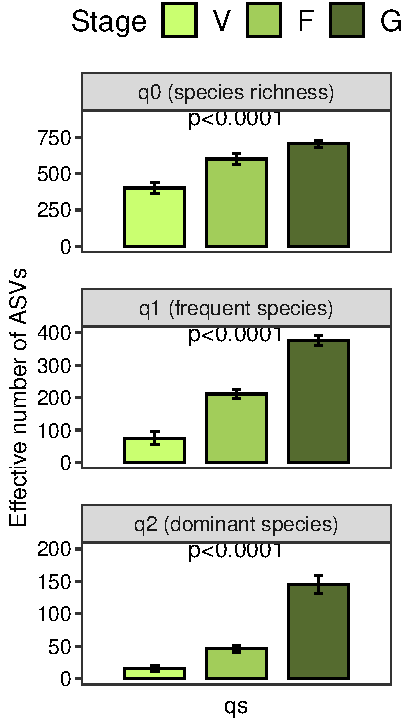
\includegraphics{Doc_pdf_files/figure-latex/unnamed-chunk-32-1} \end{center}

\begin{Shaded}
\begin{Highlighting}[]
\NormalTok{boxplot\_bulk\_stage}\OtherTok{\textless{}{-}}\FunctionTok{subset}\NormalTok{(alpha, Soil}\SpecialCharTok{==}\StringTok{"BS"}\NormalTok{) }\SpecialCharTok{\%\textgreater{}\%} 
  \FunctionTok{ggbarplot}\NormalTok{(}\AttributeTok{x=}\StringTok{"qs"}\NormalTok{, }\AttributeTok{y=}\StringTok{"value"}\NormalTok{, }\AttributeTok{fill =} \StringTok{"Stage"}\NormalTok{, }\AttributeTok{add =} \StringTok{"mean\_se"}\NormalTok{,}
            \AttributeTok{position =} \FunctionTok{position\_dodge}\NormalTok{())}\SpecialCharTok{+}
  \FunctionTok{theme\_bw}\NormalTok{()}\SpecialCharTok{+}
  \FunctionTok{labs}\NormalTok{(}\AttributeTok{y =} \StringTok{"Effective number of ASVs"}\NormalTok{)}\SpecialCharTok{+}
  \FunctionTok{facet\_wrap}\NormalTok{(}\SpecialCharTok{\textasciitilde{}}\NormalTok{qs, }\AttributeTok{scales =} \StringTok{"free"}\NormalTok{, }\AttributeTok{dir =} \StringTok{"v"}\NormalTok{)}\SpecialCharTok{+}
  \FunctionTok{theme}\NormalTok{(}\AttributeTok{panel.spacing=}\FunctionTok{unit}\NormalTok{(}\DecValTok{1}\NormalTok{,}\StringTok{"lines"}\NormalTok{),}
        \AttributeTok{strip.text.x =} \FunctionTok{element\_text}\NormalTok{(}\AttributeTok{size =} \DecValTok{10}\NormalTok{),}
        \AttributeTok{axis.text =}  \FunctionTok{element\_text}\NormalTok{(}\AttributeTok{colour =} \StringTok{"black"}\NormalTok{, }\AttributeTok{size =} \DecValTok{10}\NormalTok{),}
        \AttributeTok{axis.ticks.x=}\FunctionTok{element\_blank}\NormalTok{(), }
        \AttributeTok{legend.title =} \FunctionTok{element\_text}\NormalTok{(}\AttributeTok{size =} \DecValTok{14}\NormalTok{),}
        \AttributeTok{legend.text =} \FunctionTok{element\_text}\NormalTok{(}\AttributeTok{size=}\DecValTok{14}\NormalTok{), }
        \AttributeTok{axis.text.x =} \FunctionTok{element\_blank}\NormalTok{(),}
        \AttributeTok{panel.grid.major =} \FunctionTok{element\_blank}\NormalTok{(), }\AttributeTok{panel.grid.minor =} \FunctionTok{element\_blank}\NormalTok{(),}
        \AttributeTok{legend.direction =} \StringTok{"horizontal"}\NormalTok{ ,}
        \AttributeTok{legend.position =} \StringTok{"top"}\NormalTok{)}\SpecialCharTok{+}\FunctionTok{scale\_fill\_manual}\NormalTok{(}\AttributeTok{values =} \FunctionTok{c}\NormalTok{(}
          \StringTok{"darkolivegreen1"}\NormalTok{,}\StringTok{"darkolivegreen3"}\NormalTok{,}\StringTok{"darkolivegreen"}\NormalTok{))}\SpecialCharTok{+} \FunctionTok{labs}\NormalTok{(}\AttributeTok{fill =} \StringTok{"Stage"}\NormalTok{)}

\NormalTok{boxplot\_bulk\_stage}\OtherTok{\textless{}{-}}\NormalTok{boxplot\_bulk\_stage }\SpecialCharTok{+}  \FunctionTok{geom\_text}\NormalTok{(}\AttributeTok{data =}\NormalTok{ ann\_text,}\AttributeTok{label=}\NormalTok{ann\_text}\SpecialCharTok{$}\NormalTok{label)}

\NormalTok{boxplot\_bulk\_stage}
\end{Highlighting}
\end{Shaded}

\begin{center}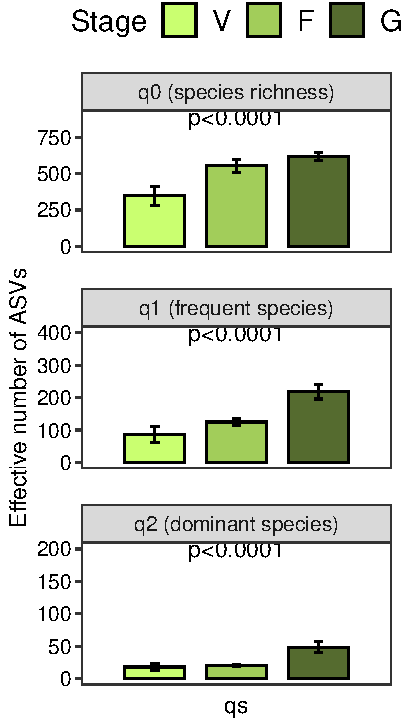
\includegraphics{Doc_pdf_files/figure-latex/unnamed-chunk-32-2} \end{center}

\begin{Shaded}
\begin{Highlighting}[]
\CommentTok{\#pdf("fig\_bulk\_stage.pdf", width=2.7, height=5)}
\CommentTok{\#print(boxplot\_bulk\_stage)}
\CommentTok{\#dev.off()}
\CommentTok{\#pdf("fig\_rhizo\_stage.pdf", width=2.7, height=5)}
\CommentTok{\#print(boxplot\_rhizo\_stage)}
\CommentTok{\#dev.off()}
\end{Highlighting}
\end{Shaded}

\begin{Shaded}
\begin{Highlighting}[]
\CommentTok{\#Functional diversity barplot }

\NormalTok{boxplot\_rhizo\_stage\_f}\OtherTok{\textless{}{-}}\FunctionTok{subset}\NormalTok{(func, Soil}\SpecialCharTok{==}\StringTok{"Rh"}\NormalTok{) }\SpecialCharTok{\%\textgreater{}\%} 
  \FunctionTok{ggbarplot}\NormalTok{(}\AttributeTok{x=}\StringTok{"fs"}\NormalTok{, }\AttributeTok{y=}\StringTok{"value"}\NormalTok{, }\AttributeTok{fill =} \StringTok{"Stage"}\NormalTok{, }\AttributeTok{add =} \StringTok{"mean\_se"}\NormalTok{,}
            \AttributeTok{position =} \FunctionTok{position\_dodge}\NormalTok{())}\SpecialCharTok{+}
  \FunctionTok{theme\_bw}\NormalTok{()}\SpecialCharTok{+}
  \FunctionTok{labs}\NormalTok{(}\AttributeTok{y =} \StringTok{"Mean functional diversity"}\NormalTok{)}\SpecialCharTok{+}
  \FunctionTok{facet\_wrap}\NormalTok{(}\SpecialCharTok{\textasciitilde{}}\NormalTok{fs, }\AttributeTok{scales =} \StringTok{"free"}\NormalTok{, }\AttributeTok{dir =} \StringTok{"v"}\NormalTok{)}\SpecialCharTok{+}
  \FunctionTok{theme}\NormalTok{(}\AttributeTok{panel.spacing=}\FunctionTok{unit}\NormalTok{(}\DecValTok{1}\NormalTok{,}\StringTok{"lines"}\NormalTok{),}
        \AttributeTok{strip.text.x =} \FunctionTok{element\_text}\NormalTok{(}\AttributeTok{size =} \DecValTok{10}\NormalTok{),}
        \AttributeTok{axis.text =}  \FunctionTok{element\_text}\NormalTok{(}\AttributeTok{colour =} \StringTok{"black"}\NormalTok{, }\AttributeTok{size =} \DecValTok{10}\NormalTok{),}
        \AttributeTok{axis.ticks.x=}\FunctionTok{element\_blank}\NormalTok{(), }
        \AttributeTok{legend.title =} \FunctionTok{element\_text}\NormalTok{(}\AttributeTok{size =} \DecValTok{14}\NormalTok{),}
        \AttributeTok{legend.text =} \FunctionTok{element\_text}\NormalTok{(}\AttributeTok{size=}\DecValTok{14}\NormalTok{), }
        \AttributeTok{axis.text.x =} \FunctionTok{element\_blank}\NormalTok{(),}
        \AttributeTok{panel.grid.major =} \FunctionTok{element\_blank}\NormalTok{(), }\AttributeTok{panel.grid.minor =} \FunctionTok{element\_blank}\NormalTok{(),}
        \AttributeTok{legend.direction =} \StringTok{"horizontal"}\NormalTok{ ,}
        \AttributeTok{legend.position =} \StringTok{"top"}\NormalTok{)}\SpecialCharTok{+}\FunctionTok{scale\_fill\_manual}\NormalTok{(}\AttributeTok{values =} \FunctionTok{c}\NormalTok{(}\StringTok{"darkolivegreen1"}\NormalTok{,}\StringTok{"darkolivegreen3"}\NormalTok{,}\StringTok{"darkolivegreen"}\NormalTok{))}\SpecialCharTok{+} \FunctionTok{labs}\NormalTok{(}\AttributeTok{fill =} \StringTok{"Stage"}\NormalTok{)}

\NormalTok{boxplot\_rhizo\_stage\_f}\OtherTok{\textless{}{-}}\NormalTok{boxplot\_rhizo\_stage\_f }\SpecialCharTok{+}  \FunctionTok{geom\_text}\NormalTok{(}\AttributeTok{data =}\NormalTok{ ann\_text\_f,}\AttributeTok{label=}\NormalTok{ann\_text\_f}\SpecialCharTok{$}\NormalTok{label)}

\NormalTok{boxplot\_rhizo\_stage\_f}
\end{Highlighting}
\end{Shaded}

\begin{center}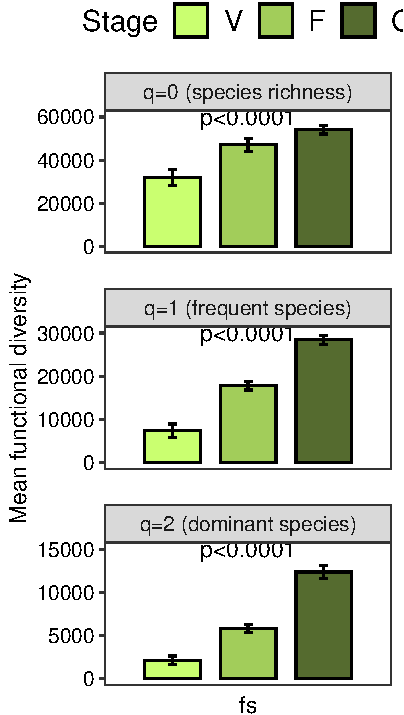
\includegraphics{Doc_pdf_files/figure-latex/unnamed-chunk-33-1} \end{center}

\begin{Shaded}
\begin{Highlighting}[]
\NormalTok{boxplot\_bulk\_stage\_f}\OtherTok{\textless{}{-}}\FunctionTok{subset}\NormalTok{(func, Soil}\SpecialCharTok{==}\StringTok{"BS"}\NormalTok{) }\SpecialCharTok{\%\textgreater{}\%} 
  \FunctionTok{ggbarplot}\NormalTok{(}\AttributeTok{x=}\StringTok{"fs"}\NormalTok{, }\AttributeTok{y=}\StringTok{"value"}\NormalTok{, }\AttributeTok{fill =} \StringTok{"Stage"}\NormalTok{, }\AttributeTok{add =} \StringTok{"mean\_se"}\NormalTok{,}
            \AttributeTok{position =} \FunctionTok{position\_dodge}\NormalTok{())}\SpecialCharTok{+}
  \FunctionTok{theme\_bw}\NormalTok{()}\SpecialCharTok{+}
  \FunctionTok{labs}\NormalTok{(}\AttributeTok{y =} \StringTok{"Mean functional diversity"}\NormalTok{)}\SpecialCharTok{+}
  \FunctionTok{facet\_wrap}\NormalTok{(}\SpecialCharTok{\textasciitilde{}}\NormalTok{fs, }\AttributeTok{scales =} \StringTok{"free"}\NormalTok{, }\AttributeTok{dir =} \StringTok{"v"}\NormalTok{)}\SpecialCharTok{+}
  \FunctionTok{theme}\NormalTok{(}\AttributeTok{panel.spacing=}\FunctionTok{unit}\NormalTok{(}\DecValTok{1}\NormalTok{,}\StringTok{"lines"}\NormalTok{),}
        \AttributeTok{strip.text.x =} \FunctionTok{element\_text}\NormalTok{(}\AttributeTok{size =} \DecValTok{10}\NormalTok{),}
        \AttributeTok{axis.text =}  \FunctionTok{element\_text}\NormalTok{(}\AttributeTok{colour =} \StringTok{"black"}\NormalTok{, }\AttributeTok{size =} \DecValTok{10}\NormalTok{),}
        \AttributeTok{axis.ticks.x=}\FunctionTok{element\_blank}\NormalTok{(), }
        \AttributeTok{legend.title =} \FunctionTok{element\_text}\NormalTok{(}\AttributeTok{size =} \DecValTok{14}\NormalTok{),}
        \AttributeTok{legend.text =} \FunctionTok{element\_text}\NormalTok{(}\AttributeTok{size=}\DecValTok{14}\NormalTok{), }
        \AttributeTok{axis.text.x =} \FunctionTok{element\_blank}\NormalTok{(),}
        \AttributeTok{panel.grid.major =} \FunctionTok{element\_blank}\NormalTok{(), }\AttributeTok{panel.grid.minor =} \FunctionTok{element\_blank}\NormalTok{(),}
        \AttributeTok{legend.direction =} \StringTok{"horizontal"}\NormalTok{ ,}
        \AttributeTok{legend.position =} \StringTok{"top"}\NormalTok{)}\SpecialCharTok{+}\FunctionTok{scale\_fill\_manual}\NormalTok{(}\AttributeTok{values =} \FunctionTok{c}\NormalTok{(}\StringTok{"darkolivegreen1"}\NormalTok{,}\StringTok{"darkolivegreen3"}\NormalTok{,}\StringTok{"darkolivegreen"}\NormalTok{))}\SpecialCharTok{+} \FunctionTok{labs}\NormalTok{(}\AttributeTok{fill =} \StringTok{"Stage"}\NormalTok{)}

\NormalTok{boxplot\_bulk\_stage\_f}\OtherTok{\textless{}{-}}\NormalTok{boxplot\_bulk\_stage\_f }\SpecialCharTok{+}  \FunctionTok{geom\_text}\NormalTok{(}\AttributeTok{data =}\NormalTok{ ann\_text\_f,}\AttributeTok{label=}\NormalTok{ann\_text\_f}\SpecialCharTok{$}\NormalTok{label)}

\NormalTok{boxplot\_bulk\_stage\_f}
\end{Highlighting}
\end{Shaded}

\begin{center}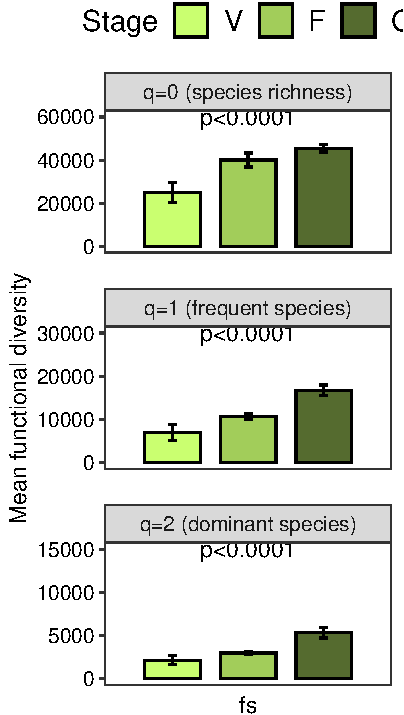
\includegraphics{Doc_pdf_files/figure-latex/unnamed-chunk-33-2} \end{center}

\begin{Shaded}
\begin{Highlighting}[]
\CommentTok{\#pdf("fig\_bulk\_stage\_f.pdf", width=2.7, height=5)}
\CommentTok{\#print(boxplot\_bulk\_stage\_f)}
\CommentTok{\#dev.off()}
\CommentTok{\#pdf("fig\_rhizo\_stage\_f.pdf", width=2.7, height=5)}
\CommentTok{\#print(boxplot\_rhizo\_stage\_f)}
\CommentTok{\#dev.off()}
\end{Highlighting}
\end{Shaded}

\hypertarget{aldex-results-heatmap-from-soil-2}{%
\subsubsection{Aldex results heatmap from
Soil}\label{aldex-results-heatmap-from-soil-2}}

\begin{Shaded}
\begin{Highlighting}[]
\CommentTok{\#function to heatmap}
\NormalTok{my\_fun }\OtherTok{\textless{}{-}} \ControlFlowTok{function}\NormalTok{(x) \{ }
\NormalTok{  x }\SpecialCharTok{\%\textgreater{}\%} \FunctionTok{separate}\NormalTok{(}
    \StringTok{"Taxon"}\NormalTok{, }\FunctionTok{c}\NormalTok{(}\StringTok{"k"}\NormalTok{, }\StringTok{"phylum"}\NormalTok{,}\StringTok{"c"}\NormalTok{, }\StringTok{"o"}\NormalTok{,}\StringTok{"f"}\NormalTok{,}\StringTok{"g"}\NormalTok{),}
    \AttributeTok{sep =} \StringTok{"}\SpecialCharTok{\textbackslash{}\textbackslash{}}\StringTok{;"}\NormalTok{, }\AttributeTok{remove =}\NormalTok{ F) }\SpecialCharTok{\%\textgreater{}\%}\NormalTok{ dplyr}\SpecialCharTok{::}\FunctionTok{select}\NormalTok{(}
\NormalTok{      Taxon, p.value, effect, diff.btw, rab.win}\FloatTok{.0}\NormalTok{, rab.win}\FloatTok{.1}\NormalTok{, phylum, }
      \StringTok{"FeatureID"}\OtherTok{=}\StringTok{"Feature.ID"}\NormalTok{ )}\SpecialCharTok{\%\textgreater{}\%} 
    \FunctionTok{drop\_na}\NormalTok{(.)}\SpecialCharTok{\%\textgreater{}\%} 
    \FunctionTok{rownames\_to\_column}\NormalTok{(}\AttributeTok{var=}\StringTok{"rows"}\NormalTok{)}\SpecialCharTok{\%\textgreater{}\%}       
    \FunctionTok{mutate\_all}\NormalTok{(}\FunctionTok{funs}\NormalTok{(}\FunctionTok{str\_replace}\NormalTok{(., }\StringTok{"k\_\_Bacteria;"}\NormalTok{, }\StringTok{""}\NormalTok{)))}\SpecialCharTok{\%\textgreater{}\%}
    \FunctionTok{mutate\_all}\NormalTok{(}\FunctionTok{funs}\NormalTok{(}\FunctionTok{str\_replace}\NormalTok{(., }\StringTok{"; c\_\_; o\_\_; f\_\_; g\_\_; s\_\_"}\NormalTok{, }\StringTok{""}\NormalTok{)))}\SpecialCharTok{\%\textgreater{}\%} 
    \FunctionTok{mutate\_all}\NormalTok{(}\FunctionTok{funs}\NormalTok{(}\FunctionTok{str\_replace}\NormalTok{(., }\StringTok{"; o\_\_; f\_\_; g\_\_; s\_\_"}\NormalTok{, }\StringTok{""}\NormalTok{)))}\SpecialCharTok{\%\textgreater{}\%} 
    \FunctionTok{mutate\_all}\NormalTok{(}\FunctionTok{funs}\NormalTok{(}\FunctionTok{str\_replace}\NormalTok{(., }\StringTok{"; f\_\_; g\_\_; s\_\_"}\NormalTok{, }\StringTok{""}\NormalTok{)))}\SpecialCharTok{\%\textgreater{}\%}
    \FunctionTok{mutate\_all}\NormalTok{(}\FunctionTok{funs}\NormalTok{(}\FunctionTok{str\_replace}\NormalTok{(., }\StringTok{"; g\_\_; s\_\_"}\NormalTok{, }\StringTok{""}\NormalTok{)))}\SpecialCharTok{\%\textgreater{}\%}
    \FunctionTok{mutate\_all}\NormalTok{(}\FunctionTok{funs}\NormalTok{(}\FunctionTok{str\_replace}\NormalTok{(., }\StringTok{"; s\_\_"}\NormalTok{, }\StringTok{""}\NormalTok{)))}\SpecialCharTok{\%\textgreater{}\%}\FunctionTok{mutate}\NormalTok{(}
      \AttributeTok{tax=} \FunctionTok{str\_extract}\NormalTok{(Taxon, }\StringTok{"[\^{}\_]+$"}\NormalTok{)) }\SpecialCharTok{\%\textgreater{}\%}\FunctionTok{mutate}\NormalTok{(}
        \AttributeTok{taxo =} \FunctionTok{paste}\NormalTok{(rows,}\StringTok{"\_"}\NormalTok{,tax))}\SpecialCharTok{\%\textgreater{}\%} \FunctionTok{mutate\_at}\NormalTok{(}
          \FunctionTok{c}\NormalTok{(}\DecValTok{3}\SpecialCharTok{:}\DecValTok{7}\NormalTok{), as.numeric) }\SpecialCharTok{\%\textgreater{}\%}
    \FunctionTok{mutate\_at}\NormalTok{(}\FunctionTok{c}\NormalTok{(}\DecValTok{3}\NormalTok{), }\FunctionTok{funs}\NormalTok{(}\AttributeTok{p.Value =} \FunctionTok{case\_when}\NormalTok{(}
\NormalTok{      . }\SpecialCharTok{\textless{}=} \FloatTok{0.001} \SpecialCharTok{\textasciitilde{}} \StringTok{"\textless{}0.001"}\NormalTok{,}
\NormalTok{      . }\SpecialCharTok{\textgreater{}}  \FloatTok{0.001} \SpecialCharTok{\&}\NormalTok{ .  }\SpecialCharTok{\textless{}=} \FloatTok{0.01} \SpecialCharTok{\textasciitilde{}} \StringTok{"\textless{}0.01"}\NormalTok{,}
\NormalTok{      . }\SpecialCharTok{\textgreater{}}  \FloatTok{0.01} \SpecialCharTok{\&}\NormalTok{ .  }\SpecialCharTok{\textless{}=} \FloatTok{0.05} \SpecialCharTok{\textasciitilde{}} \StringTok{"\textless{}0.05"}\NormalTok{)))}\SpecialCharTok{\%\textgreater{}\%}
    \FunctionTok{arrange}\NormalTok{(diff.btw)}\SpecialCharTok{\%\textgreater{}\%}\FunctionTok{column\_to\_rownames}\NormalTok{(}
      \AttributeTok{var =} \StringTok{"taxo"}\NormalTok{)}\SpecialCharTok{\%\textgreater{}\%} \FunctionTok{mutate\_at}\NormalTok{(}\FunctionTok{c}\NormalTok{(}\DecValTok{8}\NormalTok{),}\FunctionTok{funs}\NormalTok{(}\FunctionTok{str\_replace}\NormalTok{(., }\StringTok{"p\_\_"}\NormalTok{, }\StringTok{""}\NormalTok{)))\}}

\CommentTok{\#VvsF}
\CommentTok{\#file to heatmap}
\NormalTok{aldex\_all\_dif\_VvsF}\OtherTok{\textless{}{-}} \FunctionTok{read\_tsv}\NormalTok{(}\StringTok{"../Data/aldex\_all\_dif\_VvsF.tsv"}\NormalTok{)}

\NormalTok{annotation\_heatmap1 }\OtherTok{\textless{}{-}} \FunctionTok{my\_fun}\NormalTok{(aldex\_all\_dif\_VvsF) }
\NormalTok{data\_heatmap}\OtherTok{\textless{}{-}}\NormalTok{ annotation\_heatmap1}\SpecialCharTok{\%\textgreater{}\%}\NormalTok{dplyr}\SpecialCharTok{::}\FunctionTok{select}\NormalTok{(rab.win}\FloatTok{.0}\NormalTok{, rab.win}\FloatTok{.1}\NormalTok{)}

\CommentTok{\#Setting colors to heatmap}
\NormalTok{colo\_heatmap}\OtherTok{=} \FunctionTok{colorRamp2}\NormalTok{(}\FunctionTok{seq}\NormalTok{(}\FunctionTok{min}\NormalTok{(data\_heatmap), }\FunctionTok{max}\NormalTok{(}
\NormalTok{  data\_heatmap), }\AttributeTok{length =} \DecValTok{5}\NormalTok{), }\FunctionTok{c}\NormalTok{(}
    \StringTok{"\#0000FF"}\NormalTok{,}\StringTok{"\#5499C7"}\NormalTok{, }\StringTok{"\#DAE7E4"}\NormalTok{,  }\StringTok{"red"}\NormalTok{, }\StringTok{"\#FF0000"}\NormalTok{))}

\CommentTok{\#annotation phylum}
\NormalTok{cols\_ann }\OtherTok{\textless{}{-}} \FunctionTok{list}\NormalTok{(}\StringTok{\textquotesingle{}phylum\textquotesingle{}} \OtherTok{=} \FunctionTok{c}\NormalTok{(}\StringTok{" Acidobacteria"} \OtherTok{=} \StringTok{\textquotesingle{}red2\textquotesingle{}}\NormalTok{,}
                              \StringTok{" Actinobacteria"} \OtherTok{=} \StringTok{\textquotesingle{}royalblue\textquotesingle{}}\NormalTok{,}
                              \StringTok{" Bacteroidetes"}\OtherTok{=}\StringTok{"yellow"}\NormalTok{,}
                              \StringTok{" Chloroflexi"} \OtherTok{=}\StringTok{"pink"}\NormalTok{,}
                              \StringTok{" Firmicutes"}\OtherTok{=} \StringTok{"green"}\NormalTok{,}
                              \StringTok{" Gemmatimonadetes"} \OtherTok{=} \StringTok{"black"}\NormalTok{,}
                              \StringTok{" Proteobacteria"}  \OtherTok{=}\StringTok{"gray"}\NormalTok{,}
                              \StringTok{" Verrucomicrobia"} \OtherTok{=}\StringTok{"brown"}\NormalTok{, }
                              \StringTok{" Nitrospirae"} \OtherTok{=}\StringTok{"DarkGreen"}\NormalTok{, }
                              \StringTok{" TM7"}\OtherTok{=} \StringTok{"blue"}\NormalTok{, }
                              \StringTok{" Planctomycetes"} \OtherTok{=}\StringTok{"purple"}\NormalTok{))}
\NormalTok{colAnn }\OtherTok{\textless{}{-}} \FunctionTok{HeatmapAnnotation}\NormalTok{(}\AttributeTok{phylum =}\NormalTok{ annotation\_heatmap1}\SpecialCharTok{$}\NormalTok{phylum,}
                            \AttributeTok{which =} \StringTok{\textquotesingle{}row\textquotesingle{}}\NormalTok{,}
                            \AttributeTok{col =}\NormalTok{ cols\_ann,}
                            \AttributeTok{show\_legend =}\NormalTok{ T)}

\CommentTok{\#pvalue annotation}

\NormalTok{cols\_pvalue }\OtherTok{\textless{}{-}} \FunctionTok{list}\NormalTok{(}\StringTok{\textquotesingle{}p{-}value\textquotesingle{}} \OtherTok{=} \FunctionTok{c}\NormalTok{(}\StringTok{"\textless{}0.001"} \OtherTok{=} \StringTok{\textquotesingle{}\#AB0000\textquotesingle{}}\NormalTok{,}
                                  \StringTok{"\textless{}0.01"} \OtherTok{=} \StringTok{\textquotesingle{}\#FF0000\textquotesingle{}}\NormalTok{,}
                                  \StringTok{"\textless{}0.05"}\OtherTok{=}\StringTok{"\#FFB6B6"}\NormalTok{))}

\NormalTok{annP2 }\OtherTok{=} \FunctionTok{HeatmapAnnotation}\NormalTok{(}\StringTok{"p{-}value"} \OtherTok{=}\NormalTok{ annotation\_heatmap1}\SpecialCharTok{$}\NormalTok{p.Value,}
                          \AttributeTok{which =} \StringTok{"row"}\NormalTok{, }\AttributeTok{col =}\NormalTok{ cols\_pvalue,}
                          \AttributeTok{show\_legend =}\NormalTok{ T)}\CommentTok{\#, gp = gpar(col = "white"))}


\CommentTok{\#effect annotation}
\NormalTok{effect\_col\_fun }\OtherTok{=}\FunctionTok{colorRamp2}\NormalTok{(}\FunctionTok{c}\NormalTok{(}\SpecialCharTok{{-}}\FloatTok{1.5}\NormalTok{, }\DecValTok{0}\NormalTok{, }\FloatTok{1.5}\NormalTok{), }\FunctionTok{c}\NormalTok{(}
  \StringTok{"lightsalmon4"}\NormalTok{, }\StringTok{"white"}\NormalTok{, }\StringTok{"lightseagreen"}\NormalTok{))}

\NormalTok{annEffect }\OtherTok{=} \FunctionTok{HeatmapAnnotation}\NormalTok{(}\StringTok{"effect{-}size"} \OtherTok{=}\NormalTok{ annotation\_heatmap1}\SpecialCharTok{$}\NormalTok{effect,}
                              \AttributeTok{which =} \StringTok{"row"}\NormalTok{, }\AttributeTok{col =} \FunctionTok{list}\NormalTok{(}\StringTok{"effect{-}size"} \OtherTok{=}\NormalTok{ effect\_col\_fun),}
                              \AttributeTok{show\_legend =}\NormalTok{ T, }
                              \AttributeTok{gp =} \FunctionTok{gpar}\NormalTok{(}\AttributeTok{col =} \StringTok{"white"}\NormalTok{))}
\CommentTok{\#barplot annotation}
\NormalTok{bardif}\OtherTok{=} \FunctionTok{rowAnnotation}\NormalTok{(}
  \StringTok{"difference }\SpecialCharTok{\textbackslash{}n}\StringTok{ between groups"} \OtherTok{=} \FunctionTok{anno\_barplot}\NormalTok{(}
\NormalTok{    annotation\_heatmap1}\SpecialCharTok{$}\NormalTok{diff.btw, }\AttributeTok{width =} \FunctionTok{unit}\NormalTok{(}\DecValTok{4}\NormalTok{, }\StringTok{"cm"}\NormalTok{)))}

\NormalTok{labels1 }\OtherTok{=}\NormalTok{ (annotation\_heatmap1}\SpecialCharTok{$}\NormalTok{tax)}

\NormalTok{htVvsF}\OtherTok{\textless{}{-}}\NormalTok{  ComplexHeatmap}\SpecialCharTok{::}\FunctionTok{Heatmap}\NormalTok{(}
  \FunctionTok{as.matrix}\NormalTok{(data\_heatmap), }\AttributeTok{col =}\NormalTok{ colo\_heatmap, }\AttributeTok{row\_dend\_reorder =}\NormalTok{ F,                                   }\AttributeTok{width =} \FunctionTok{ncol}\NormalTok{(data\_heatmap)}\SpecialCharTok{*}\FunctionTok{unit}\NormalTok{(}\DecValTok{1}\NormalTok{, }\StringTok{"cm"}\NormalTok{),}
  \AttributeTok{height =} \FunctionTok{ncol}\NormalTok{(data\_heatmap)}\SpecialCharTok{*}\FunctionTok{unit}\NormalTok{(}\FloatTok{1.4}\NormalTok{, }\StringTok{"cm"}\NormalTok{),}
  \AttributeTok{left\_annotation =}  \FunctionTok{c}\NormalTok{(annP2,annEffect, colAnn),}
  \AttributeTok{heatmap\_legend\_param =} \FunctionTok{list}\NormalTok{(}\AttributeTok{direction =} \StringTok{"horizontal"}\NormalTok{ ),}
  \AttributeTok{right\_annotation =} \FunctionTok{c}\NormalTok{(bardif),}
  \AttributeTok{column\_split =} \FunctionTok{factor}\NormalTok{(}\FunctionTok{rep}\NormalTok{(}\FunctionTok{c}\NormalTok{(}\StringTok{"V"}\NormalTok{, }\StringTok{"F"}\NormalTok{)), }\AttributeTok{levels =} \FunctionTok{c}\NormalTok{(}\StringTok{"V"}\NormalTok{, }\StringTok{"F"}\NormalTok{)),}
  \AttributeTok{cluster\_rows =}\NormalTok{ F, }\AttributeTok{column\_km =} \DecValTok{1}\NormalTok{, }
  \AttributeTok{column\_title\_gp =} \FunctionTok{gpar}\NormalTok{(}\AttributeTok{fill =} \FunctionTok{c}\NormalTok{(}\StringTok{"darkolivegreen1"}\NormalTok{,}\StringTok{"darkolivegreen3"}\NormalTok{), }\AttributeTok{col=}\StringTok{"white"}\NormalTok{),}
  \AttributeTok{border =}\NormalTok{ F, }\AttributeTok{column\_gap =} \FunctionTok{unit}\NormalTok{(}\FloatTok{0.5}\NormalTok{, }\StringTok{"mm"}\NormalTok{), }\AttributeTok{row\_dend\_side =} \StringTok{"left"}\NormalTok{,}
  \AttributeTok{row\_names\_side =} \StringTok{"right"}\NormalTok{,}\AttributeTok{show\_row\_names =}\NormalTok{ F ,}
  \AttributeTok{rect\_gp =} \FunctionTok{gpar}\NormalTok{(}\AttributeTok{col =} \StringTok{"white"}\NormalTok{, }\AttributeTok{lwd =} \FloatTok{0.2}\NormalTok{), }\AttributeTok{row\_names\_gp =} \FunctionTok{gpar}\NormalTok{(}
  \AttributeTok{fontface =}\StringTok{"italic"}\NormalTok{, }\AttributeTok{fontsize=}\DecValTok{10}\NormalTok{),}\AttributeTok{show\_column\_names =}\NormalTok{ F, }\AttributeTok{name =} \StringTok{"rab.Win"}\NormalTok{,}
  \AttributeTok{cluster\_column\_slices =}\NormalTok{ F) }\SpecialCharTok{+}\FunctionTok{rowAnnotation}\NormalTok{(}\AttributeTok{labels =} \FunctionTok{anno\_text}\NormalTok{(}
\NormalTok{  labels1, }\AttributeTok{which =} \StringTok{"row"}\NormalTok{, }\FunctionTok{gpar}\NormalTok{(}\AttributeTok{col =} \StringTok{"black"}\NormalTok{, }\AttributeTok{fontsize =} \DecValTok{6}\NormalTok{)),}\AttributeTok{width =} \FunctionTok{unit}\NormalTok{(}\DecValTok{2}\NormalTok{, }\StringTok{"cm"}\NormalTok{))}


\NormalTok{htVvsF}
\end{Highlighting}
\end{Shaded}

\begin{center}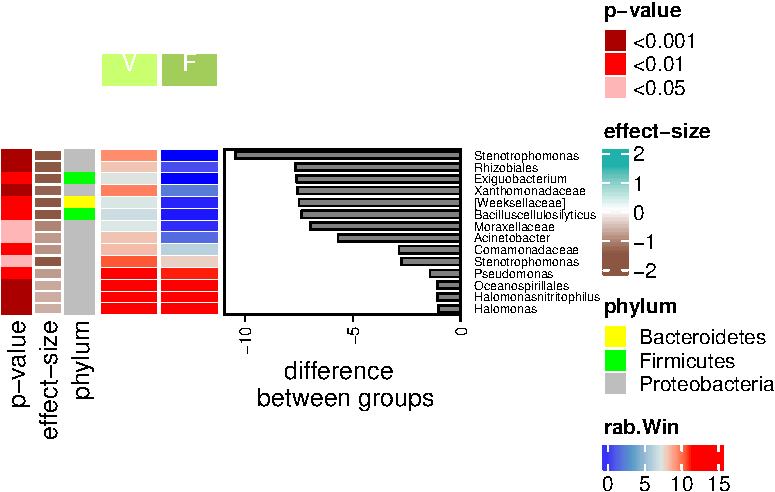
\includegraphics{Doc_pdf_files/figure-latex/unnamed-chunk-34-1} \end{center}

\begin{Shaded}
\begin{Highlighting}[]
\CommentTok{\#pdf("fig\_aldex\_VvsF.pdf", width=6, height=5)}
\CommentTok{\#print(htVvsF)}
\CommentTok{\#dev.off()}

\NormalTok{htVvsF}\FloatTok{.2}\OtherTok{\textless{}{-}}\FunctionTok{draw}\NormalTok{(htVvsF, }\AttributeTok{heatmap\_legend\_side =} \StringTok{"bottom"}\NormalTok{, }
               \AttributeTok{annotation\_legend\_side =} \StringTok{"bottom"}\NormalTok{)}
\end{Highlighting}
\end{Shaded}

\begin{center}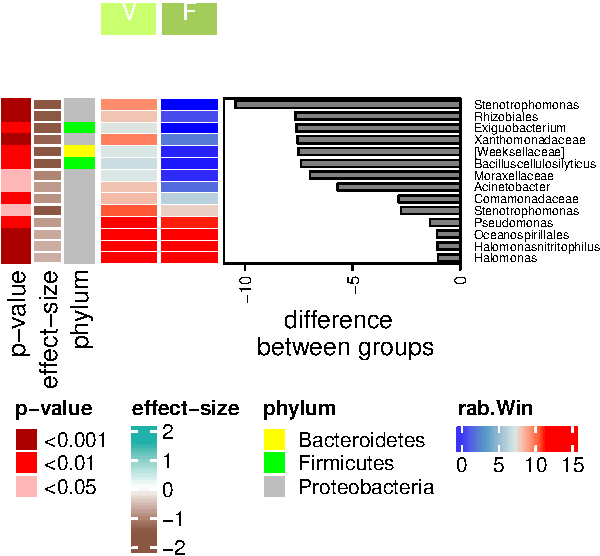
\includegraphics{Doc_pdf_files/figure-latex/unnamed-chunk-34-2} \end{center}

\begin{Shaded}
\begin{Highlighting}[]
\CommentTok{\#pdf("fig\_aldex\_VvsF2.pdf", width=6, height=6)}
\CommentTok{\#print(htVvsF.2)}
\CommentTok{\#dev.off()}


\CommentTok{\#FVSG}
\CommentTok{\#loading file}
\NormalTok{aldex\_all\_dif\_FvsG}\OtherTok{\textless{}{-}}\FunctionTok{read\_tsv}\NormalTok{(}\StringTok{"../Data/aldex\_all\_dif\_FvsG.tsv"}\NormalTok{)}

\NormalTok{annotation\_heatmap2 }\OtherTok{\textless{}{-}} \FunctionTok{my\_fun}\NormalTok{(aldex\_all\_dif\_FvsG) }
\NormalTok{data\_heatmap}\OtherTok{\textless{}{-}}\NormalTok{ annotation\_heatmap2}\SpecialCharTok{\%\textgreater{}\%}\NormalTok{dplyr}\SpecialCharTok{::}\FunctionTok{select}\NormalTok{(rab.win}\FloatTok{.0}\NormalTok{, rab.win}\FloatTok{.1}\NormalTok{)}

\CommentTok{\#Setting colors to heatmap}
\NormalTok{colo\_heatmap}\OtherTok{=} \FunctionTok{colorRamp2}\NormalTok{(}\FunctionTok{seq}\NormalTok{(}\FunctionTok{min}\NormalTok{(data\_heatmap), }\FunctionTok{max}\NormalTok{(data\_heatmap),}
\AttributeTok{length =} \DecValTok{5}\NormalTok{), }\FunctionTok{c}\NormalTok{(}\StringTok{"\#0000FF"}\NormalTok{,}\StringTok{"\#5499C7"}\NormalTok{, }\StringTok{"\#DAE7E4"}\NormalTok{,  }\StringTok{"red"}\NormalTok{, }\StringTok{"\#FF0000"}\NormalTok{))}

\CommentTok{\#annotation phylum}
\NormalTok{cols\_ann }\OtherTok{\textless{}{-}} \FunctionTok{list}\NormalTok{(}\StringTok{\textquotesingle{}phylum\textquotesingle{}} \OtherTok{=} \FunctionTok{c}\NormalTok{(}
  \StringTok{" Acidobacteria"} \OtherTok{=} \StringTok{\textquotesingle{}red2\textquotesingle{}}\NormalTok{,}
  \StringTok{" Actinobacteria"} \OtherTok{=} \StringTok{\textquotesingle{}royalblue\textquotesingle{}}\NormalTok{,}
  \StringTok{" Bacteroidetes"}\OtherTok{=}\StringTok{"yellow"}\NormalTok{,}
  \StringTok{" Chloroflexi"} \OtherTok{=}\StringTok{"pink"}\NormalTok{,}
  \StringTok{" Firmicutes"}\OtherTok{=} \StringTok{"green"}\NormalTok{,}
  \StringTok{" Gemmatimonadetes"} \OtherTok{=} \StringTok{"black"}\NormalTok{,}
  \StringTok{" Proteobacteria"}  \OtherTok{=}\StringTok{"gray"}\NormalTok{,}
  \StringTok{" Verrucomicrobia"} \OtherTok{=}\StringTok{"brown"}\NormalTok{, }
  \StringTok{" TM7"}\OtherTok{=} \StringTok{"blue"}\NormalTok{, }
  \StringTok{" Planctomycetes"} \OtherTok{=}\StringTok{"purple"}\NormalTok{))}

\NormalTok{colAnn }\OtherTok{\textless{}{-}} \FunctionTok{HeatmapAnnotation}\NormalTok{(}\AttributeTok{phylum =}\NormalTok{ annotation\_heatmap2}\SpecialCharTok{$}\NormalTok{phylum,}
                            \AttributeTok{which =} \StringTok{\textquotesingle{}row\textquotesingle{}}\NormalTok{,}
                            \AttributeTok{col =}\NormalTok{ cols\_ann,}
                            \AttributeTok{show\_legend =}\NormalTok{ F)}


\CommentTok{\#pvalue annotation}

\NormalTok{cols\_pvalue }\OtherTok{\textless{}{-}} \FunctionTok{list}\NormalTok{(}\StringTok{\textquotesingle{}p{-}value\textquotesingle{}} \OtherTok{=} \FunctionTok{c}\NormalTok{(}\StringTok{"\textless{}0.001"} \OtherTok{=} \StringTok{\textquotesingle{}\#AB0000\textquotesingle{}}\NormalTok{,}
                                  \StringTok{"\textless{}0.01"} \OtherTok{=} \StringTok{\textquotesingle{}\#FF0000\textquotesingle{}}\NormalTok{,}
                                  \StringTok{"\textless{}0.05"}\OtherTok{=}\StringTok{"\#FFB6B6"}\NormalTok{))}

\NormalTok{annP2 }\OtherTok{=} \FunctionTok{HeatmapAnnotation}\NormalTok{(}\StringTok{"p{-}value"} \OtherTok{=}\NormalTok{ annotation\_heatmap2}\SpecialCharTok{$}\NormalTok{p.Value,}
                          \AttributeTok{which =} \StringTok{"row"}\NormalTok{, }\AttributeTok{col =}\NormalTok{ cols\_pvalue,}
                          \AttributeTok{show\_legend =}\NormalTok{ F)}

\CommentTok{\#effect annotation}
\NormalTok{effect\_col\_fun }\OtherTok{=}\FunctionTok{colorRamp2}\NormalTok{(}\FunctionTok{c}\NormalTok{(}\SpecialCharTok{{-}}\FloatTok{1.5}\NormalTok{, }\DecValTok{0}\NormalTok{, }\FloatTok{1.5}\NormalTok{), }\FunctionTok{c}\NormalTok{(}
  \StringTok{"lightsalmon4"}\NormalTok{, }\StringTok{"white"}\NormalTok{, }\StringTok{"lightseagreen"}\NormalTok{))}

\NormalTok{annEffect }\OtherTok{=} \FunctionTok{HeatmapAnnotation}\NormalTok{(}\StringTok{"effect{-}size"} \OtherTok{=}\NormalTok{ annotation\_heatmap2}\SpecialCharTok{$}\NormalTok{effect,}
                              \AttributeTok{which =} \StringTok{"row"}\NormalTok{, }\AttributeTok{col =} \FunctionTok{list}\NormalTok{(}
                                \StringTok{"effect{-}size"} \OtherTok{=}\NormalTok{ effect\_col\_fun),}
                              \AttributeTok{show\_legend =}\NormalTok{ F, }
                              \AttributeTok{gp =} \FunctionTok{gpar}\NormalTok{(}\AttributeTok{col =} \StringTok{"white"}\NormalTok{))}

\CommentTok{\#barplot annotation}
\NormalTok{bardif}\OtherTok{=} \FunctionTok{rowAnnotation}\NormalTok{(}
  \StringTok{"difference }\SpecialCharTok{\textbackslash{}n}\StringTok{ between groups"} \OtherTok{=} \FunctionTok{anno\_barplot}\NormalTok{(}
\NormalTok{    annotation\_heatmap2}\SpecialCharTok{$}\NormalTok{diff.btw, }\AttributeTok{width =} \FunctionTok{unit}\NormalTok{(}\DecValTok{4}\NormalTok{, }\StringTok{"cm"}\NormalTok{)))}

\NormalTok{labels2 }\OtherTok{=}\NormalTok{ (annotation\_heatmap2}\SpecialCharTok{$}\NormalTok{tax)}

\NormalTok{htFvsG}\OtherTok{\textless{}{-}}\NormalTok{ComplexHeatmap}\SpecialCharTok{::}\FunctionTok{Heatmap}\NormalTok{(}
\NormalTok{  data\_heatmap, }\AttributeTok{col =}\NormalTok{ colo\_heatmap, }\AttributeTok{row\_dend\_reorder =}\NormalTok{ F, }
  \AttributeTok{width =} \FunctionTok{ncol}\NormalTok{(data\_heatmap)}\SpecialCharTok{*}\FunctionTok{unit}\NormalTok{(}\DecValTok{1}\NormalTok{, }\StringTok{"cm"}\NormalTok{),}
  \AttributeTok{height =} \FunctionTok{ncol}\NormalTok{(data\_heatmap)}\SpecialCharTok{*}\FunctionTok{unit}\NormalTok{(}\DecValTok{1}\NormalTok{, }\StringTok{"cm"}\NormalTok{),}
  \AttributeTok{left\_annotation =}  \FunctionTok{c}\NormalTok{(annP2, annEffect, colAnn),}
  \AttributeTok{heatmap\_legend\_param =} \FunctionTok{list}\NormalTok{(}\AttributeTok{direction =} \StringTok{"horizontal"}\NormalTok{ ),}
  \AttributeTok{right\_annotation =} \FunctionTok{c}\NormalTok{(bardif),}
  \AttributeTok{column\_split =} \FunctionTok{rep}\NormalTok{(}\FunctionTok{c}\NormalTok{(}\StringTok{"F"}\NormalTok{, }\StringTok{"G"}\NormalTok{)),}
  \AttributeTok{cluster\_rows =}\NormalTok{ F, }\AttributeTok{show\_heatmap\_legend =}\NormalTok{ F,}
  \AttributeTok{cluster\_column\_slices =}\NormalTok{ F,}
  \AttributeTok{column\_km =} \DecValTok{1}\NormalTok{, }\AttributeTok{column\_title\_gp =} \FunctionTok{gpar}\NormalTok{(}
  \AttributeTok{fill =} \FunctionTok{c}\NormalTok{(}\StringTok{"darkolivegreen3"}\NormalTok{,}\StringTok{"darkolivegreen"}\NormalTok{), }\AttributeTok{col=}\StringTok{"white"}\NormalTok{),}
  \AttributeTok{border =}\NormalTok{ F, }\AttributeTok{column\_gap =} \FunctionTok{unit}\NormalTok{(}\FloatTok{0.5}\NormalTok{, }\StringTok{"mm"}\NormalTok{), }
  \AttributeTok{row\_dend\_side =} \StringTok{"left"}\NormalTok{,}\AttributeTok{row\_names\_side =} \StringTok{"right"}\NormalTok{,}\AttributeTok{show\_row\_names =}\NormalTok{ F ,}
  \AttributeTok{rect\_gp =} \FunctionTok{gpar}\NormalTok{(}\AttributeTok{col =} \StringTok{"white"}\NormalTok{, }\AttributeTok{lwd =} \FloatTok{0.2}\NormalTok{), }\AttributeTok{row\_names\_gp =} \FunctionTok{gpar}\NormalTok{(}
  \AttributeTok{fontface =}\StringTok{"italic"}\NormalTok{, }\AttributeTok{fontsize=}\DecValTok{10}\NormalTok{),}\AttributeTok{show\_column\_names =}\NormalTok{ F, }
  \AttributeTok{name =} \StringTok{"rab.Win"}\NormalTok{)}\SpecialCharTok{+}  \FunctionTok{rowAnnotation}\NormalTok{(}
    \AttributeTok{labels =} \FunctionTok{anno\_text}\NormalTok{(labels2, }\AttributeTok{which =} \StringTok{"row"}\NormalTok{, }\FunctionTok{gpar}\NormalTok{(}
  \AttributeTok{col =} \StringTok{"black"}\NormalTok{, }\AttributeTok{fontsize =} \DecValTok{6}\NormalTok{)), }\AttributeTok{width =} \FunctionTok{unit}\NormalTok{(}\DecValTok{2}\NormalTok{, }\StringTok{"cm"}\NormalTok{))}

\NormalTok{htFvsG}
\end{Highlighting}
\end{Shaded}

\begin{center}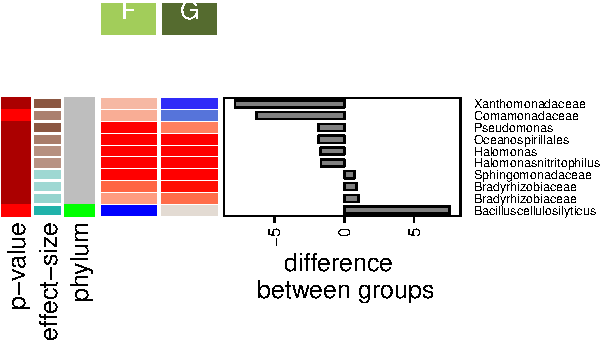
\includegraphics{Doc_pdf_files/figure-latex/unnamed-chunk-34-3} \end{center}

\begin{Shaded}
\begin{Highlighting}[]
\CommentTok{\#pdf("fig\_aldex\_FvsG.pdf", width=6, height=5)}
\CommentTok{\#print(htFvsG)}
\CommentTok{\#dev.off()}

\CommentTok{\# VvsG}

\NormalTok{aldex\_all\_dif\_VvsG}\OtherTok{\textless{}{-}}\FunctionTok{read\_tsv}\NormalTok{(}\StringTok{"../Data/aldex\_all\_dif\_VvsG.tsv"}\NormalTok{)}
\NormalTok{annotation\_heatmap3 }\OtherTok{\textless{}{-}} \FunctionTok{my\_fun}\NormalTok{(aldex\_all\_dif\_VvsG) }
\NormalTok{data\_heatmap}\OtherTok{\textless{}{-}}\NormalTok{ annotation\_heatmap3}\SpecialCharTok{\%\textgreater{}\%}\NormalTok{dplyr}\SpecialCharTok{::}\FunctionTok{select}\NormalTok{(rab.win}\FloatTok{.0}\NormalTok{, rab.win}\FloatTok{.1}\NormalTok{)}

\CommentTok{\#Setting colors to heatmap}
\NormalTok{colo\_heatmap}\OtherTok{=} \FunctionTok{colorRamp2}\NormalTok{(}\FunctionTok{seq}\NormalTok{(}\FunctionTok{min}\NormalTok{(data\_heatmap), }\FunctionTok{max}\NormalTok{(data\_heatmap),}
\AttributeTok{length =} \DecValTok{5}\NormalTok{), }\FunctionTok{c}\NormalTok{(}\StringTok{"\#0000FF"}\NormalTok{,}\StringTok{"\#5499C7"}\NormalTok{, }\StringTok{"\#DAE7E4"}\NormalTok{,  }\StringTok{"red"}\NormalTok{, }\StringTok{"\#FF0000"}\NormalTok{))}

\CommentTok{\#annotation phylum}
\NormalTok{cols\_ann }\OtherTok{\textless{}{-}} \FunctionTok{list}\NormalTok{(}\StringTok{\textquotesingle{}phylum\textquotesingle{}} \OtherTok{=} \FunctionTok{c}\NormalTok{(}
  \StringTok{" Acidobacteria"} \OtherTok{=} \StringTok{\textquotesingle{}red2\textquotesingle{}}\NormalTok{,}
  \StringTok{" Actinobacteria"} \OtherTok{=} \StringTok{\textquotesingle{}royalblue\textquotesingle{}}\NormalTok{,}
  \StringTok{" Bacteroidetes"}\OtherTok{=}\StringTok{"yellow"}\NormalTok{,}
  \StringTok{" Chloroflexi"} \OtherTok{=}\StringTok{"pink"}\NormalTok{,}
  \StringTok{" Firmicutes"}\OtherTok{=} \StringTok{"green"}\NormalTok{,}
  \StringTok{" Gemmatimonadetes"} \OtherTok{=} \StringTok{"black"}\NormalTok{,}
  \StringTok{" Proteobacteria"}  \OtherTok{=}\StringTok{"gray"}\NormalTok{,}
  \StringTok{" Verrucomicrobia"} \OtherTok{=}\StringTok{"brown"}\NormalTok{, }
  \StringTok{" TM7"}\OtherTok{=} \StringTok{"blue"}\NormalTok{, }
  \StringTok{" Planctomycetes"} \OtherTok{=}\StringTok{"purple"}\NormalTok{))}

\NormalTok{colAnn }\OtherTok{\textless{}{-}} \FunctionTok{HeatmapAnnotation}\NormalTok{(}\AttributeTok{phylum =}\NormalTok{ annotation\_heatmap3}\SpecialCharTok{$}\NormalTok{phylum,}
                            \AttributeTok{which =} \StringTok{\textquotesingle{}row\textquotesingle{}}\NormalTok{,}
                            \AttributeTok{col =}\NormalTok{ cols\_ann,}
                            \AttributeTok{show\_legend =}\NormalTok{ F)}

\CommentTok{\#pvalue annotation}

\NormalTok{cols\_pvalue }\OtherTok{\textless{}{-}} \FunctionTok{list}\NormalTok{(}\StringTok{\textquotesingle{}p{-}value\textquotesingle{}} \OtherTok{=} \FunctionTok{c}\NormalTok{(}\StringTok{"\textless{}0.001"} \OtherTok{=} \StringTok{\textquotesingle{}\#AB0000\textquotesingle{}}\NormalTok{,}
                                  \StringTok{"\textless{}0.01"} \OtherTok{=} \StringTok{\textquotesingle{}\#FF0000\textquotesingle{}}\NormalTok{,}
                                  \StringTok{"\textless{}0.05"}\OtherTok{=}\StringTok{"\#FFB6B6"}\NormalTok{))}

\NormalTok{annP2 }\OtherTok{=} \FunctionTok{HeatmapAnnotation}\NormalTok{(}\StringTok{"p{-}value"} \OtherTok{=}\NormalTok{ annotation\_heatmap3}\SpecialCharTok{$}\NormalTok{p.Value,}
                          \AttributeTok{which =} \StringTok{"row"}\NormalTok{, }\AttributeTok{col =}\NormalTok{ cols\_pvalue,}
                          \AttributeTok{show\_legend =}\NormalTok{ F)}\CommentTok{\#, gp = gpar(col = "white"))}


\CommentTok{\#effect annotation}
\NormalTok{effect\_col\_fun }\OtherTok{=}\FunctionTok{colorRamp2}\NormalTok{(}\FunctionTok{c}\NormalTok{(}\SpecialCharTok{{-}}\FloatTok{1.5}\NormalTok{, }\DecValTok{0}\NormalTok{, }\FloatTok{1.5}\NormalTok{), }\FunctionTok{c}\NormalTok{(}
  \StringTok{"lightsalmon4"}\NormalTok{, }\StringTok{"white"}\NormalTok{, }\StringTok{"lightseagreen"}\NormalTok{))}

\NormalTok{annEffect }\OtherTok{=} \FunctionTok{HeatmapAnnotation}\NormalTok{(}\StringTok{"effect{-}size"} \OtherTok{=}\NormalTok{ annotation\_heatmap3}\SpecialCharTok{$}\NormalTok{effect,}
                              \AttributeTok{which =} \StringTok{"row"}\NormalTok{, }
                              \AttributeTok{col =} \FunctionTok{list}\NormalTok{(}\StringTok{"effect{-}size"} \OtherTok{=}\NormalTok{ effect\_col\_fun),}
                              \AttributeTok{show\_legend =}\NormalTok{ F, }
                              \AttributeTok{gp =} \FunctionTok{gpar}\NormalTok{(}\AttributeTok{col =} \StringTok{"white"}\NormalTok{))}
\CommentTok{\#barplot annotation}
\NormalTok{bardif}\OtherTok{=} \FunctionTok{rowAnnotation}\NormalTok{(}
  \StringTok{"difference }\SpecialCharTok{\textbackslash{}n}\StringTok{ between groups"} \OtherTok{=} \FunctionTok{anno\_barplot}\NormalTok{(}
\NormalTok{    annotation\_heatmap3}\SpecialCharTok{$}\NormalTok{diff.btw, }\AttributeTok{width =} \FunctionTok{unit}\NormalTok{(}\DecValTok{4}\NormalTok{, }\StringTok{"cm"}\NormalTok{)))}

\NormalTok{labels3 }\OtherTok{=}\NormalTok{ (annotation\_heatmap3}\SpecialCharTok{$}\NormalTok{tax)}

\NormalTok{htVvsG}\OtherTok{\textless{}{-}}\NormalTok{ComplexHeatmap}\SpecialCharTok{::}\FunctionTok{Heatmap}\NormalTok{(}
\NormalTok{  data\_heatmap, }\AttributeTok{col =}\NormalTok{ colo\_heatmap, }\AttributeTok{row\_dend\_reorder =}\NormalTok{ F, }
  \AttributeTok{width =} \FunctionTok{ncol}\NormalTok{(data\_heatmap)}\SpecialCharTok{*}\FunctionTok{unit}\NormalTok{(}\DecValTok{1}\NormalTok{, }\StringTok{"cm"}\NormalTok{),}
  \AttributeTok{height =} \FunctionTok{ncol}\NormalTok{(data\_heatmap)}\SpecialCharTok{*}\FunctionTok{unit}\NormalTok{(}\FloatTok{1.4}\NormalTok{, }\StringTok{"cm"}\NormalTok{),}
  \AttributeTok{left\_annotation =}  \FunctionTok{c}\NormalTok{(annP2, annEffect, colAnn),}
  \AttributeTok{heatmap\_legend\_param =} \FunctionTok{list}\NormalTok{(}\AttributeTok{direction =} \StringTok{"horizontal"}\NormalTok{ ),}
  \AttributeTok{right\_annotation =} \FunctionTok{c}\NormalTok{(bardif),}
  \AttributeTok{column\_split =} \FunctionTok{factor}\NormalTok{(}\FunctionTok{rep}\NormalTok{(}\FunctionTok{c}\NormalTok{(}\StringTok{"V"}\NormalTok{, }\StringTok{"G"}\NormalTok{)), }\AttributeTok{levels =} \FunctionTok{c}\NormalTok{(}\StringTok{"V"}\NormalTok{, }\StringTok{"G"}\NormalTok{)),}
  \AttributeTok{cluster\_rows =}\NormalTok{ F,}\AttributeTok{show\_heatmap\_legend =}\NormalTok{ F,}
  \AttributeTok{column\_km =} \DecValTok{1}\NormalTok{, }\AttributeTok{column\_title\_gp =} \FunctionTok{gpar}\NormalTok{(}\AttributeTok{fill =} \FunctionTok{c}\NormalTok{(}
 \StringTok{"darkolivegreen1"}\NormalTok{,}\StringTok{"darkolivegreen"}\NormalTok{), }\AttributeTok{col=}\StringTok{"white"}\NormalTok{),}
 \AttributeTok{border =}\NormalTok{ F, }\AttributeTok{column\_gap =} \FunctionTok{unit}\NormalTok{(}\FloatTok{0.5}\NormalTok{, }\StringTok{"mm"}\NormalTok{), }
 \AttributeTok{row\_dend\_side =} \StringTok{"left"}\NormalTok{,}\AttributeTok{row\_names\_side =} \StringTok{"right"}\NormalTok{,}\AttributeTok{show\_row\_names =}\NormalTok{ F ,}
 \AttributeTok{rect\_gp =} \FunctionTok{gpar}\NormalTok{(}\AttributeTok{col =} \StringTok{"white"}\NormalTok{, }\AttributeTok{lwd =} \FloatTok{0.2}\NormalTok{), }\AttributeTok{row\_names\_gp =} \FunctionTok{gpar}\NormalTok{(}
\AttributeTok{fontface =}\StringTok{"italic"}\NormalTok{, }\AttributeTok{fontsize=}\DecValTok{10}\NormalTok{),}\AttributeTok{show\_column\_names =}\NormalTok{ F, }\AttributeTok{name =} \StringTok{"rab.Win"}\NormalTok{)}\SpecialCharTok{+}
\FunctionTok{rowAnnotation}\NormalTok{(}\AttributeTok{labels =} \FunctionTok{anno\_text}\NormalTok{(labels3, }\AttributeTok{which =} \StringTok{"row"}\NormalTok{, }
\FunctionTok{gpar}\NormalTok{(}\AttributeTok{col =} \StringTok{"black"}\NormalTok{, }\AttributeTok{fontsize =} \DecValTok{6}\NormalTok{)),}\AttributeTok{width =} \FunctionTok{unit}\NormalTok{(}\DecValTok{2}\NormalTok{, }\StringTok{"cm"}\NormalTok{))}

\CommentTok{\#pdf("fig\_aldex\_VvsG.pdf", width=6, height=5)}
\CommentTok{\#print(htVvsG)}
\CommentTok{\#dev.off()}
\end{Highlighting}
\end{Shaded}

\hypertarget{pca-plot-2}{%
\subsubsection{PCA plot}\label{pca-plot-2}}

\begin{Shaded}
\begin{Highlighting}[]
\CommentTok{\#loading files and formatting}
\NormalTok{d.pro}\FloatTok{.0}\OtherTok{\textless{}{-}} \FunctionTok{read\_tsv}\NormalTok{(}\StringTok{"../Data/otutable.tsv"}\NormalTok{) }\SpecialCharTok{\%\textgreater{}\%} \FunctionTok{column\_to\_rownames}\NormalTok{(}\AttributeTok{var =} \StringTok{"\#OTU ID"}\NormalTok{)}

\NormalTok{meta}\OtherTok{\textless{}{-}}\FunctionTok{read\_tsv}\NormalTok{(}\StringTok{"../Data/metadata.tsv"}\NormalTok{)}

\NormalTok{meta}\SpecialCharTok{$}\NormalTok{Stage}\OtherTok{\textless{}{-}} \FunctionTok{factor}\NormalTok{(meta}\SpecialCharTok{$}\NormalTok{Maize\_development\_stage,}
                    \AttributeTok{levels =} \FunctionTok{c}\NormalTok{( }\StringTok{"Vegetative"}\NormalTok{, }\StringTok{"Flowering"}\NormalTok{, }\StringTok{"Grainfilling"}\NormalTok{),}
                    \AttributeTok{labels =} \FunctionTok{c}\NormalTok{(}\StringTok{"V"}\NormalTok{, }\StringTok{"F"}\NormalTok{, }\StringTok{"G"}\NormalTok{))}

\NormalTok{tax2}\OtherTok{\textless{}{-}} \FunctionTok{read\_tsv}\NormalTok{(}\StringTok{"../Data/taxonomy.tsv"}\NormalTok{)}\SpecialCharTok{\%\textgreater{}\%} \FunctionTok{rename}\NormalTok{(}
    \StringTok{"FeatureID"}\OtherTok{=}\StringTok{\textasciigrave{}}\AttributeTok{\#OTU ID}\StringTok{\textasciigrave{}}\NormalTok{, }\AttributeTok{Taxon=}\NormalTok{ taxonomy)}

\NormalTok{tax3}\OtherTok{\textless{}{-}}\NormalTok{tax2}\SpecialCharTok{\%\textgreater{}\%} \FunctionTok{separate}\NormalTok{(}
  \StringTok{"Taxon"}\NormalTok{, }\FunctionTok{c}\NormalTok{(}\StringTok{"k"}\NormalTok{, }\StringTok{"phylum"}\NormalTok{,}\StringTok{"c"}\NormalTok{, }\StringTok{"o"}\NormalTok{,}\StringTok{"f"}\NormalTok{,}\StringTok{"g"}\NormalTok{),}
  \AttributeTok{sep =} \StringTok{"}\SpecialCharTok{\textbackslash{}\textbackslash{}}\StringTok{;"}\NormalTok{, }\AttributeTok{remove =}\NormalTok{ F) }\SpecialCharTok{\%\textgreater{}\%}
  \FunctionTok{rownames\_to\_column}\NormalTok{(}\AttributeTok{var=}\StringTok{"rows"}\NormalTok{)}\SpecialCharTok{\%\textgreater{}\%}       
  \FunctionTok{mutate\_all}\NormalTok{(}\FunctionTok{funs}\NormalTok{(}\FunctionTok{str\_replace}\NormalTok{(., }\StringTok{"k\_\_Bacteria;"}\NormalTok{, }\StringTok{""}\NormalTok{)))}\SpecialCharTok{\%\textgreater{}\%}
  \FunctionTok{mutate\_all}\NormalTok{(}\FunctionTok{funs}\NormalTok{(}\FunctionTok{str\_replace}\NormalTok{(., }\StringTok{"; c\_\_; o\_\_; f\_\_; g\_\_; s\_\_"}\NormalTok{, }\StringTok{""}\NormalTok{)))}\SpecialCharTok{\%\textgreater{}\%} 
  \FunctionTok{mutate\_all}\NormalTok{(}\FunctionTok{funs}\NormalTok{(}\FunctionTok{str\_replace}\NormalTok{(., }\StringTok{"; o\_\_; f\_\_; g\_\_; s\_\_"}\NormalTok{, }\StringTok{""}\NormalTok{)))}\SpecialCharTok{\%\textgreater{}\%} 
  \FunctionTok{mutate\_all}\NormalTok{(}\FunctionTok{funs}\NormalTok{(}\FunctionTok{str\_replace}\NormalTok{(., }\StringTok{"; f\_\_; g\_\_; s\_\_"}\NormalTok{, }\StringTok{""}\NormalTok{)))}\SpecialCharTok{\%\textgreater{}\%}
  \FunctionTok{mutate\_all}\NormalTok{(}\FunctionTok{funs}\NormalTok{(}\FunctionTok{str\_replace}\NormalTok{(., }\StringTok{"; g\_\_; s\_\_"}\NormalTok{, }\StringTok{""}\NormalTok{)))}\SpecialCharTok{\%\textgreater{}\%}
  \FunctionTok{mutate\_all}\NormalTok{(}\FunctionTok{funs}\NormalTok{(}\FunctionTok{str\_replace}\NormalTok{(., }\StringTok{"; s\_\_"}\NormalTok{, }\StringTok{""}\NormalTok{)))}\SpecialCharTok{\%\textgreater{}\%}\FunctionTok{mutate}\NormalTok{(}
    \AttributeTok{tax=} \FunctionTok{str\_extract}\NormalTok{(Taxon, }\StringTok{"[\^{}\_]+$"}\NormalTok{)) }

\NormalTok{sample\_to\_choose}\OtherTok{\textless{}{-}}\NormalTok{ meta }\SpecialCharTok{\%\textgreater{}\%} \FunctionTok{filter}\NormalTok{(Soil\_sample}\SpecialCharTok{==}\StringTok{"Rhizosphere"}\NormalTok{)}

\CommentTok{\#transforming data}
\NormalTok{d.pro.}\FloatTok{0.}\NormalTok{rhizo}\OtherTok{\textless{}{-}}\NormalTok{ d.pro}\FloatTok{.0}  \SpecialCharTok{\%\textgreater{}\%}\NormalTok{ dplyr}\SpecialCharTok{::}\FunctionTok{select}\NormalTok{(}\DecValTok{0}\NormalTok{, sample\_to\_choose}\SpecialCharTok{$}\NormalTok{SampleID)}
\NormalTok{d.pro.rhizo }\OtherTok{\textless{}{-}} \FunctionTok{t}\NormalTok{(}\FunctionTok{cmultRepl}\NormalTok{(}\FunctionTok{t}\NormalTok{(d.pro.}\FloatTok{0.}\NormalTok{rhizo), }\AttributeTok{method=}\StringTok{"CZM"}\NormalTok{, }\AttributeTok{output=}\StringTok{"p{-}counts"}\NormalTok{))}
\NormalTok{d.clr.abund.codaseq.rhizo}\OtherTok{\textless{}{-}}\FunctionTok{codaSeq.clr}\NormalTok{(}\AttributeTok{x =}\NormalTok{ d.pro.rhizo,}\AttributeTok{samples.by.row =}\NormalTok{ F)}

\CommentTok{\#run pca}
\NormalTok{pcx.abund.rhizo }\OtherTok{\textless{}{-}} \FunctionTok{prcomp}\NormalTok{(}\FunctionTok{t}\NormalTok{(d.clr.abund.codaseq.rhizo))}

\CommentTok{\#labels to pca axis}

\NormalTok{PC1 }\OtherTok{\textless{}{-}} \FunctionTok{paste}\NormalTok{(}
  \StringTok{"PC1"}\NormalTok{, }\FunctionTok{round}\NormalTok{(}\FunctionTok{sum}\NormalTok{(pcx.abund.rhizo}\SpecialCharTok{$}\NormalTok{sdev[}\DecValTok{1}\NormalTok{] }\SpecialCharTok{\^{}} \DecValTok{2}\NormalTok{) }\SpecialCharTok{/} \FunctionTok{mvar}\NormalTok{(d.clr.abund.codaseq.rhizo) , }\DecValTok{1}\NormalTok{), }\StringTok{"\%"}\NormalTok{)}
\NormalTok{PC2 }\OtherTok{\textless{}{-}} \FunctionTok{paste}\NormalTok{(}
  \StringTok{"PC2"}\NormalTok{, }\FunctionTok{round}\NormalTok{(}\FunctionTok{sum}\NormalTok{(pcx.abund.rhizo}\SpecialCharTok{$}\NormalTok{sdev[}\DecValTok{2}\NormalTok{] }\SpecialCharTok{\^{}} \DecValTok{2}\NormalTok{) }\SpecialCharTok{/} \FunctionTok{mvar}\NormalTok{(d.clr.abund.codaseq.rhizo) , }\DecValTok{1}\NormalTok{), }\StringTok{"\%"}\NormalTok{)}

\CommentTok{\#let\textquotesingle{}s choose som of the significant groups from aldex analysis }

\NormalTok{annot\_heat}\OtherTok{\textless{}{-}} \FunctionTok{merge}\NormalTok{(annotation\_heatmap1, }
\NormalTok{                   annotation\_heatmap2, }\AttributeTok{by =} \StringTok{"FeatureID"}\NormalTok{) }\SpecialCharTok{\%\textgreater{}\%}\FunctionTok{full\_join}\NormalTok{(}
\NormalTok{                     annotation\_heatmap3, }\AttributeTok{by =} \StringTok{"FeatureID"}\NormalTok{)}

\NormalTok{vars\_chosen}\OtherTok{\textless{}{-}} \FunctionTok{c}\NormalTok{(}\StringTok{"d0dbf2a66c655edf1f45eb0fe9415866"}\NormalTok{, }
                \StringTok{"2553e8df6ec901e443d9f4ed5f7ea2fe"}\NormalTok{,}
                \StringTok{"008e9d51155f32838e58a5a6eb48f335"}\NormalTok{ , }
                \CommentTok{\#"61d320df173b3b20ac4bb8a0b9adcb3c", }
                \StringTok{"f35cd29ecc2c92909b596ad30084ea48"}\NormalTok{,}
                \StringTok{"f75c3dab2258512ada2c3af6f86e5865"}\NormalTok{,}
                \StringTok{"cf75802eef23e2082bcb012af233a01b"}\NormalTok{) }
                \CommentTok{\# "3882df43374c4d647c02bb95fc46c3ed", }
                \CommentTok{\#"2553e8df6ec901e443d9f4ed5f7ea2fe", }
                \CommentTok{\#"087cf9bebbcc26a354bc475125443455")}
\CommentTok{\#these ones were chosen from before (some aldex significant groups)}

\NormalTok{vars\_to\_choose}\OtherTok{\textless{}{-}}\NormalTok{ annotation\_heatmap3 }\SpecialCharTok{\%\textgreater{}\%}  \FunctionTok{rownames\_to\_column}\NormalTok{(}
  \AttributeTok{var =} \StringTok{"ids"}\NormalTok{)}\SpecialCharTok{\%\textgreater{}\%}\FunctionTok{filter}\NormalTok{(FeatureID }\SpecialCharTok{\%in\%}\NormalTok{ vars\_chosen)}

\NormalTok{vars\_choosing}\OtherTok{\textless{}{-}} \FunctionTok{data.frame}\NormalTok{(}
\NormalTok{  pcx.abund.rhizo}\SpecialCharTok{$}\NormalTok{rotation) }\SpecialCharTok{\%\textgreater{}\%}  \FunctionTok{rownames\_to\_column}\NormalTok{(}
    \AttributeTok{var =} \StringTok{"FeatureID"}\NormalTok{)}\SpecialCharTok{\%\textgreater{}\%}   
  \FunctionTok{mutate}\NormalTok{(}\AttributeTok{a=}\FunctionTok{sqrt}\NormalTok{(PC1}\SpecialCharTok{\^{}}\DecValTok{2}\SpecialCharTok{+}\NormalTok{PC2}\SpecialCharTok{\^{}}\DecValTok{2}\NormalTok{)) }\SpecialCharTok{\%\textgreater{}\%}
  \FunctionTok{mutate}\NormalTok{(}\AttributeTok{PC1=}\NormalTok{PC1}\SpecialCharTok{*}\DecValTok{500}\NormalTok{, }\AttributeTok{PC2=}\NormalTok{PC2}\SpecialCharTok{*}\DecValTok{500}\NormalTok{) }\SpecialCharTok{\%\textgreater{}\%}\NormalTok{ dplyr}\SpecialCharTok{::}\FunctionTok{select}\NormalTok{(}
\NormalTok{    PC1, PC2, FeatureID)}\SpecialCharTok{\%\textgreater{}\%}\FunctionTok{right\_join}\NormalTok{(vars\_to\_choose, }\AttributeTok{by =} \StringTok{"FeatureID"}\NormalTok{)}

\CommentTok{\#pca{-}plot}
\NormalTok{pca\_stage\_arrows}\OtherTok{\textless{}{-}} \FunctionTok{ggplot}\NormalTok{() }\SpecialCharTok{+}
  \FunctionTok{theme\_bw}\NormalTok{() }\SpecialCharTok{+}
  \FunctionTok{xlab}\NormalTok{(PC1) }\SpecialCharTok{+}
  \FunctionTok{ylab}\NormalTok{(PC2) }\SpecialCharTok{+}
    \FunctionTok{theme}\NormalTok{(}\AttributeTok{axis.text =} \FunctionTok{element\_text}\NormalTok{(}\AttributeTok{colour =} \StringTok{"black"}\NormalTok{, }\AttributeTok{size =} \DecValTok{14}\NormalTok{), }\CommentTok{\#setting themes}
        \AttributeTok{axis.title =} \FunctionTok{element\_text}\NormalTok{(}\AttributeTok{colour =} \StringTok{"black"}\NormalTok{, }\AttributeTok{size =} \DecValTok{14}\NormalTok{),}
        \AttributeTok{legend.text =} \FunctionTok{element\_text}\NormalTok{(}\AttributeTok{size =} \DecValTok{14}\NormalTok{),}
        \AttributeTok{legend.title =} \FunctionTok{element\_blank}\NormalTok{(), }
        \AttributeTok{legend.position =} \StringTok{"bottom"}\NormalTok{, }
        \AttributeTok{legend.box =} \StringTok{"horizontal"}\NormalTok{, }
        \AttributeTok{legend.direction =} \StringTok{"horizontal"}\NormalTok{) }\SpecialCharTok{+}
  \FunctionTok{geom\_point}\NormalTok{(                              }\CommentTok{\#individuals}
    \AttributeTok{data=}\FunctionTok{data.frame}\NormalTok{(pcx.abund.rhizo}\SpecialCharTok{$}\NormalTok{x) }\SpecialCharTok{\%\textgreater{}\%}   \FunctionTok{rownames\_to\_column}\NormalTok{(}\AttributeTok{var =} \StringTok{"SampleID"}\NormalTok{)}\SpecialCharTok{\%\textgreater{}\%}
    \FunctionTok{left\_join}\NormalTok{(meta, }\AttributeTok{by =} \StringTok{"SampleID"}\NormalTok{),}
    \FunctionTok{aes}\NormalTok{(}\AttributeTok{x=}\NormalTok{PC1, }\AttributeTok{y=}\NormalTok{PC2, }\AttributeTok{fill=}\NormalTok{Stage), }
    \AttributeTok{shape=}\DecValTok{21}\NormalTok{, }\AttributeTok{size=}\DecValTok{4}\NormalTok{) }\SpecialCharTok{+} 
  \FunctionTok{geom\_vline}\NormalTok{(}\AttributeTok{xintercept =} \DecValTok{0}\NormalTok{, }\AttributeTok{linetype =} \DecValTok{2}\NormalTok{) }\SpecialCharTok{+}   \CommentTok{\#lines{-}cross}
  \FunctionTok{geom\_hline}\NormalTok{(}\AttributeTok{yintercept =} \DecValTok{0}\NormalTok{, }\AttributeTok{linetype =} \DecValTok{2}\NormalTok{) }\SpecialCharTok{+}
  \FunctionTok{scale\_fill\_manual}\NormalTok{(}\AttributeTok{values =} \FunctionTok{c}\NormalTok{( }\StringTok{"darkolivegreen1"}\NormalTok{,}\StringTok{"darkolivegreen3"}\NormalTok{,}\StringTok{"darkolivegreen"}\NormalTok{))}\SpecialCharTok{+}
\NormalTok{  ggrepel}\SpecialCharTok{::}\FunctionTok{geom\_label\_repel}\NormalTok{(}\AttributeTok{data =}\NormalTok{ vars\_choosing, }\FunctionTok{aes}\NormalTok{(}\AttributeTok{x=}\NormalTok{PC1, }\AttributeTok{y=}\NormalTok{PC2, }\AttributeTok{label=}\NormalTok{ tax),}
                            \AttributeTok{segment.colour =} \ConstantTok{NA}\NormalTok{, }\AttributeTok{box.padding =} \DecValTok{2}\NormalTok{, }\AttributeTok{fontface=}\StringTok{"italic"}\NormalTok{)}\SpecialCharTok{+}
  \FunctionTok{geom\_segment}\NormalTok{(}\AttributeTok{data =}\NormalTok{ vars\_choosing, }\FunctionTok{aes}\NormalTok{(}\AttributeTok{x =} \DecValTok{0}\NormalTok{, }\AttributeTok{y =} \DecValTok{0}\NormalTok{, }\AttributeTok{xend =}\NormalTok{ PC1, }\AttributeTok{yend =}\NormalTok{ PC2), }
               \AttributeTok{arrow=}\FunctionTok{arrow}\NormalTok{(}\AttributeTok{length=}\FunctionTok{unit}\NormalTok{(}\FloatTok{0.15}\NormalTok{,}\StringTok{"cm"}\NormalTok{)), }\CommentTok{\#arros and names}
               \AttributeTok{alpha =} \FloatTok{0.75}\NormalTok{, }\AttributeTok{color =} \StringTok{\textquotesingle{}black\textquotesingle{}}\NormalTok{, }\AttributeTok{size=} \FloatTok{0.6}\NormalTok{)}

\NormalTok{pca\_stage\_arrows}
\end{Highlighting}
\end{Shaded}

\begin{center}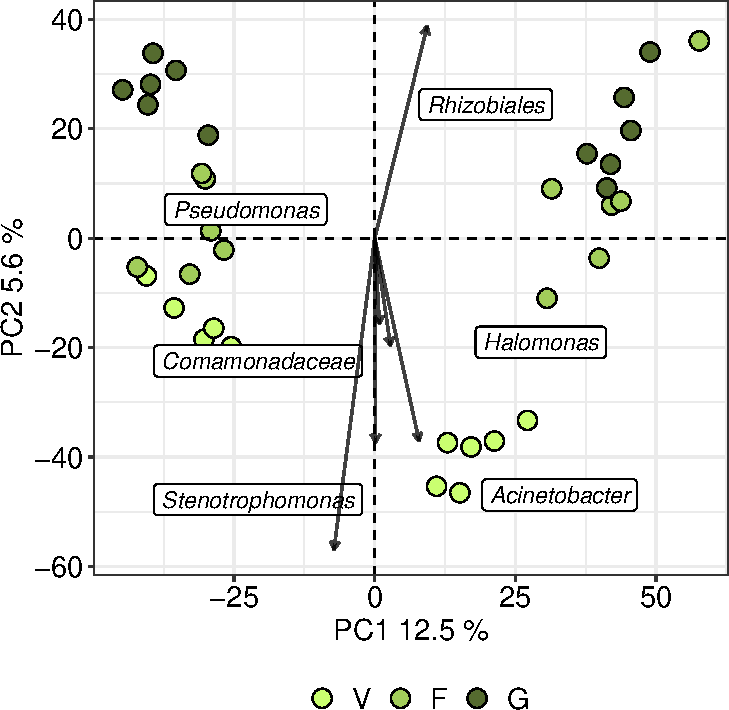
\includegraphics{Doc_pdf_files/figure-latex/unnamed-chunk-35-1} \end{center}

\begin{Shaded}
\begin{Highlighting}[]
\CommentTok{\#pdf("fig\_PCA\_rhizo\_stage.pdf", width=5, height=5)}
\CommentTok{\#print(pca\_stage\_arrows)}
\CommentTok{\#dev.off()}
\end{Highlighting}
\end{Shaded}

\begin{Shaded}
\begin{Highlighting}[]
\CommentTok{\# PCA VEGETATIVE STAGE}

\NormalTok{sample\_to\_choose\_v}\OtherTok{\textless{}{-}}\NormalTok{ meta }\SpecialCharTok{\%\textgreater{}\%} \FunctionTok{filter}\NormalTok{(Stage}\SpecialCharTok{==}\StringTok{"V"}\NormalTok{)}
\NormalTok{d.pro.}\FloatTok{0.}\NormalTok{V}\OtherTok{\textless{}{-}}\NormalTok{ d.pro}\FloatTok{.0}  \SpecialCharTok{\%\textgreater{}\%}\NormalTok{ dplyr}\SpecialCharTok{::}\FunctionTok{select}\NormalTok{(}\DecValTok{0}\NormalTok{, sample\_to\_choose\_v}\SpecialCharTok{$}\NormalTok{SampleID)}
\NormalTok{d.pro.V }\OtherTok{\textless{}{-}} \FunctionTok{t}\NormalTok{(}\FunctionTok{cmultRepl}\NormalTok{(}\FunctionTok{t}\NormalTok{(d.pro.}\FloatTok{0.}\NormalTok{V), }\AttributeTok{method=}\StringTok{"CZM"}\NormalTok{, }\AttributeTok{output=}\StringTok{"p{-}counts"}\NormalTok{)) }\CommentTok{\#tratamiento de 0}

\NormalTok{d.clr.abund.codaseq.V}\OtherTok{\textless{}{-}}\FunctionTok{codaSeq.clr}\NormalTok{(}\AttributeTok{x =}\NormalTok{ d.pro.V, }\AttributeTok{samples.by.row =}\NormalTok{ F) }\CommentTok{\#transformacion clr}

\NormalTok{pcx.abund.V }\OtherTok{\textless{}{-}} \FunctionTok{prcomp}\NormalTok{(}\FunctionTok{t}\NormalTok{(d.clr.abund.codaseq.V))}



\NormalTok{PC1 }\OtherTok{\textless{}{-}} \FunctionTok{paste}\NormalTok{(}
  \StringTok{"PC1"}\NormalTok{, }\FunctionTok{round}\NormalTok{(}\FunctionTok{sum}\NormalTok{(pcx.abund.V}\SpecialCharTok{$}\NormalTok{sdev[}\DecValTok{1}\NormalTok{] }\SpecialCharTok{\^{}} \DecValTok{2}\NormalTok{) }\SpecialCharTok{/} \FunctionTok{mvar}\NormalTok{(d.clr.abund.codaseq.V), }\DecValTok{1}\NormalTok{), }\StringTok{"\%"}\NormalTok{)}
\NormalTok{PC2 }\OtherTok{\textless{}{-}} \FunctionTok{paste}\NormalTok{(}
  \StringTok{"PC2"}\NormalTok{, }\FunctionTok{round}\NormalTok{(}\FunctionTok{sum}\NormalTok{(pcx.abund.V}\SpecialCharTok{$}\NormalTok{sdev[}\DecValTok{2}\NormalTok{] }\SpecialCharTok{\^{}} \DecValTok{2}\NormalTok{) }\SpecialCharTok{/} \FunctionTok{mvar}\NormalTok{(d.clr.abund.codaseq.V) , }\DecValTok{1}\NormalTok{), }\StringTok{"\%"}\NormalTok{)}

\NormalTok{vars\_choosing}\OtherTok{\textless{}{-}} \FunctionTok{data.frame}\NormalTok{(pcx.abund.V}\SpecialCharTok{$}\NormalTok{rotation) }\SpecialCharTok{\%\textgreater{}\%}  \FunctionTok{rownames\_to\_column}\NormalTok{(}\AttributeTok{var =} \StringTok{"FeatureID"}\NormalTok{)}\SpecialCharTok{\%\textgreater{}\%}   
  \FunctionTok{mutate}\NormalTok{(}\AttributeTok{a=}\FunctionTok{sqrt}\NormalTok{(PC1}\SpecialCharTok{\^{}}\DecValTok{2}\SpecialCharTok{+}\NormalTok{PC2}\SpecialCharTok{\^{}}\DecValTok{2}\NormalTok{)) }\SpecialCharTok{\%\textgreater{}\%}
  \FunctionTok{mutate}\NormalTok{(}\AttributeTok{PC1=}\NormalTok{PC1}\SpecialCharTok{*}\DecValTok{500}\NormalTok{, }\AttributeTok{PC2=}\NormalTok{PC2}\SpecialCharTok{*}\DecValTok{500}\NormalTok{) }\SpecialCharTok{\%\textgreater{}\%} \FunctionTok{top\_n}\NormalTok{(}\DecValTok{8}\NormalTok{, a) }\SpecialCharTok{\%\textgreater{}\%}\NormalTok{ dplyr}\SpecialCharTok{::}\FunctionTok{select}\NormalTok{(}
\NormalTok{    PC1, PC2, FeatureID) }\SpecialCharTok{\%\textgreater{}\%} \FunctionTok{right\_join}\NormalTok{(tax3, }\AttributeTok{by =} \StringTok{"FeatureID"}\NormalTok{)}

\CommentTok{\#pca{-}plot}
\NormalTok{pca\_stage\_arrows\_V}\OtherTok{\textless{}{-}} \FunctionTok{ggplot}\NormalTok{() }\SpecialCharTok{+}
  \FunctionTok{theme\_bw}\NormalTok{() }\SpecialCharTok{+}
  \FunctionTok{xlab}\NormalTok{(PC1) }\SpecialCharTok{+}
  \FunctionTok{ylab}\NormalTok{(PC2) }\SpecialCharTok{+}
  \FunctionTok{theme}\NormalTok{(}\AttributeTok{axis.text =} \FunctionTok{element\_text}\NormalTok{(}\AttributeTok{colour =} \StringTok{"black"}\NormalTok{, }\AttributeTok{size =} \DecValTok{14}\NormalTok{), }\CommentTok{\#setting theme}
        \AttributeTok{axis.title =} \FunctionTok{element\_text}\NormalTok{(}\AttributeTok{colour =} \StringTok{"black"}\NormalTok{, }\AttributeTok{size =} \DecValTok{14}\NormalTok{),}
        \AttributeTok{legend.text =} \FunctionTok{element\_text}\NormalTok{(}\AttributeTok{size =} \DecValTok{14}\NormalTok{),}
        \AttributeTok{legend.title =} \FunctionTok{element\_blank}\NormalTok{(), }
        \AttributeTok{legend.position =} \StringTok{"bottom"}\NormalTok{, }
        \AttributeTok{legend.box =} \StringTok{"horizontal"}\NormalTok{, }
        \AttributeTok{legend.direction =} \StringTok{"horizontal"}\NormalTok{) }\SpecialCharTok{+}
  \FunctionTok{geom\_point}\NormalTok{(                              }\CommentTok{\#individuals}
    \AttributeTok{data=}\FunctionTok{data.frame}\NormalTok{(pcx.abund.V}\SpecialCharTok{$}\NormalTok{x) }\SpecialCharTok{\%\textgreater{}\%}   \FunctionTok{rownames\_to\_column}\NormalTok{(}\AttributeTok{var =} \StringTok{"SampleID"}\NormalTok{)}\SpecialCharTok{\%\textgreater{}\%}
      \FunctionTok{left\_join}\NormalTok{(meta, }\AttributeTok{by =} \StringTok{"SampleID"}\NormalTok{),}
    \FunctionTok{aes}\NormalTok{(}\AttributeTok{x=}\NormalTok{PC1, }\AttributeTok{y=}\NormalTok{PC2, }\AttributeTok{fill=}\NormalTok{Soil\_sample), }
    \AttributeTok{shape=}\DecValTok{21}\NormalTok{, }\AttributeTok{size=}\DecValTok{4}\NormalTok{) }\SpecialCharTok{+}
  \FunctionTok{geom\_vline}\NormalTok{(}\AttributeTok{xintercept =} \DecValTok{0}\NormalTok{, }\AttributeTok{linetype =} \DecValTok{2}\NormalTok{) }\SpecialCharTok{+}   \CommentTok{\#lines{-}cross}
  \FunctionTok{geom\_hline}\NormalTok{(}\AttributeTok{yintercept =} \DecValTok{0}\NormalTok{, }\AttributeTok{linetype =} \DecValTok{2}\NormalTok{) }\SpecialCharTok{+}
  \FunctionTok{scale\_fill\_manual}\NormalTok{(}\AttributeTok{values =} \FunctionTok{c}\NormalTok{(}\StringTok{"darkgoldenrod4"}\NormalTok{, }\StringTok{"\#365238"}\NormalTok{))}\SpecialCharTok{+}
\NormalTok{  ggrepel}\SpecialCharTok{::}\FunctionTok{geom\_label\_repel}\NormalTok{(}\AttributeTok{data =}\NormalTok{ vars\_choosing, }\FunctionTok{aes}\NormalTok{(}\AttributeTok{x=}\NormalTok{PC1, }\AttributeTok{y=}\NormalTok{PC2, }\AttributeTok{label=}\NormalTok{ tax),}
                            \AttributeTok{segment.colour =} \ConstantTok{NA}\NormalTok{, }\AttributeTok{box.padding =} \DecValTok{2}\NormalTok{, }\AttributeTok{fontface=}\StringTok{"italic"}\NormalTok{)}\SpecialCharTok{+}
  \FunctionTok{geom\_segment}\NormalTok{(}\AttributeTok{data =}\NormalTok{ vars\_choosing, }\FunctionTok{aes}\NormalTok{(}\AttributeTok{x =} \DecValTok{0}\NormalTok{, }\AttributeTok{y =} \DecValTok{0}\NormalTok{, }\AttributeTok{xend =}\NormalTok{ PC1, }\AttributeTok{yend =}\NormalTok{ PC2), }
               \AttributeTok{arrow=}\FunctionTok{arrow}\NormalTok{(}\AttributeTok{length=}\FunctionTok{unit}\NormalTok{(}\FloatTok{0.15}\NormalTok{,}\StringTok{"cm"}\NormalTok{)), }\CommentTok{\#arrows and names}
               \AttributeTok{alpha =} \FloatTok{0.75}\NormalTok{, }\AttributeTok{color =} \StringTok{\textquotesingle{}black\textquotesingle{}}\NormalTok{, }\AttributeTok{size=} \FloatTok{0.6}\NormalTok{)}

\NormalTok{pca\_stage\_arrows\_V}
\end{Highlighting}
\end{Shaded}

\begin{center}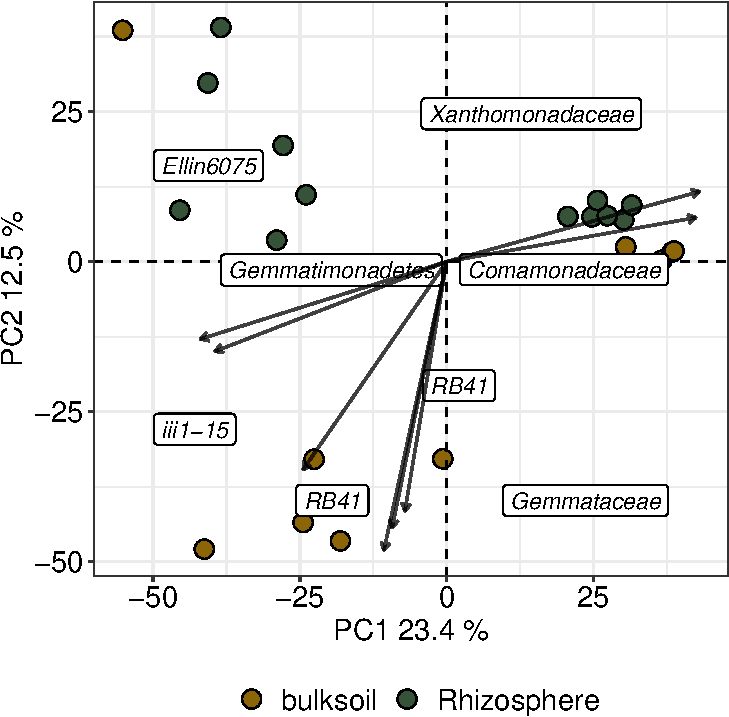
\includegraphics{Doc_pdf_files/figure-latex/unnamed-chunk-36-1} \end{center}

\begin{Shaded}
\begin{Highlighting}[]
\CommentTok{\#pdf("fig\_PCA\_vegetative.pdf", width=5, height=5)}
\CommentTok{\#print(pca\_stage\_arrows\_V)}
\CommentTok{\#dev.off()}
\end{Highlighting}
\end{Shaded}

\begin{Shaded}
\begin{Highlighting}[]
\CommentTok{\# PCA FLOWERING STAGE}

\NormalTok{sample\_to\_choose\_f}\OtherTok{\textless{}{-}}\NormalTok{ meta }\SpecialCharTok{\%\textgreater{}\%} \FunctionTok{filter}\NormalTok{(Stage}\SpecialCharTok{==}\StringTok{"F"}\NormalTok{)}
\NormalTok{d.pro.}\FloatTok{0.}\NormalTok{F}\OtherTok{\textless{}{-}}\NormalTok{ d.pro}\FloatTok{.0}  \SpecialCharTok{\%\textgreater{}\%}\NormalTok{ dplyr}\SpecialCharTok{::}\FunctionTok{select}\NormalTok{(}\DecValTok{0}\NormalTok{, sample\_to\_choose\_f}\SpecialCharTok{$}\NormalTok{SampleID)}
\NormalTok{d.pro.F }\OtherTok{\textless{}{-}} \FunctionTok{t}\NormalTok{(}\FunctionTok{cmultRepl}\NormalTok{(}\FunctionTok{t}\NormalTok{(d.pro.}\FloatTok{0.}\NormalTok{F), }\AttributeTok{method=}\StringTok{"CZM"}\NormalTok{, }\AttributeTok{output=}\StringTok{"p{-}counts"}\NormalTok{)) }\CommentTok{\#tratamiento de 0}

\NormalTok{d.clr.abund.codaseq.F}\OtherTok{\textless{}{-}}\FunctionTok{codaSeq.clr}\NormalTok{(}\AttributeTok{x =}\NormalTok{ d.pro.F, }\AttributeTok{samples.by.row =}\NormalTok{ F) }\CommentTok{\#transformacion clr}

\NormalTok{pcx.abund.F }\OtherTok{\textless{}{-}} \FunctionTok{prcomp}\NormalTok{(}\FunctionTok{t}\NormalTok{(d.clr.abund.codaseq.F))}


\NormalTok{PC1 }\OtherTok{\textless{}{-}} \FunctionTok{paste}\NormalTok{(}
  \StringTok{"PC1"}\NormalTok{, }\FunctionTok{round}\NormalTok{(}\FunctionTok{sum}\NormalTok{(pcx.abund.F}\SpecialCharTok{$}\NormalTok{sdev[}\DecValTok{1}\NormalTok{] }\SpecialCharTok{\^{}} \DecValTok{2}\NormalTok{) }\SpecialCharTok{/} \FunctionTok{mvar}\NormalTok{(d.clr.abund.codaseq.F) }\SpecialCharTok{*} \DecValTok{100}\NormalTok{, }\DecValTok{1}\NormalTok{), }\StringTok{"\%"}\NormalTok{)}
\NormalTok{PC2 }\OtherTok{\textless{}{-}} \FunctionTok{paste}\NormalTok{(}
  \StringTok{"PC2"}\NormalTok{, }\FunctionTok{round}\NormalTok{(}\FunctionTok{sum}\NormalTok{(pcx.abund.F}\SpecialCharTok{$}\NormalTok{sdev[}\DecValTok{2}\NormalTok{] }\SpecialCharTok{\^{}} \DecValTok{2}\NormalTok{) }\SpecialCharTok{/} \FunctionTok{mvar}\NormalTok{(d.clr.abund.codaseq.F) }\SpecialCharTok{*} \DecValTok{100}\NormalTok{, }\DecValTok{1}\NormalTok{), }\StringTok{"\%"}\NormalTok{)}

\NormalTok{vars\_choosing}\OtherTok{\textless{}{-}} \FunctionTok{data.frame}\NormalTok{(pcx.abund.F}\SpecialCharTok{$}\NormalTok{rotation) }\SpecialCharTok{\%\textgreater{}\%}  \FunctionTok{rownames\_to\_column}\NormalTok{(}\AttributeTok{var =} \StringTok{"FeatureID"}\NormalTok{)}\SpecialCharTok{\%\textgreater{}\%}   
  \FunctionTok{mutate}\NormalTok{(}\AttributeTok{a=}\FunctionTok{sqrt}\NormalTok{(PC1}\SpecialCharTok{\^{}}\DecValTok{2}\SpecialCharTok{+}\NormalTok{PC2}\SpecialCharTok{\^{}}\DecValTok{2}\NormalTok{)) }\SpecialCharTok{\%\textgreater{}\%}
  \FunctionTok{mutate}\NormalTok{(}\AttributeTok{PC1=}\NormalTok{PC1}\SpecialCharTok{*}\DecValTok{500}\NormalTok{, }\AttributeTok{PC2=}\NormalTok{PC2}\SpecialCharTok{*}\DecValTok{500}\NormalTok{) }\SpecialCharTok{\%\textgreater{}\%} \FunctionTok{top\_n}\NormalTok{(}\DecValTok{8}\NormalTok{, a) }\SpecialCharTok{\%\textgreater{}\%}\NormalTok{ dplyr}\SpecialCharTok{::}\FunctionTok{select}\NormalTok{(}
\NormalTok{    PC1, PC2, FeatureID) }\SpecialCharTok{\%\textgreater{}\%} \FunctionTok{right\_join}\NormalTok{(tax3, }\AttributeTok{by =} \StringTok{"FeatureID"}\NormalTok{)}

\CommentTok{\#create the base plot with only the arrows}
\NormalTok{pca\_stage\_arrows\_F}\OtherTok{\textless{}{-}} \FunctionTok{ggplot}\NormalTok{() }\SpecialCharTok{+}
  \FunctionTok{theme\_bw}\NormalTok{() }\SpecialCharTok{+}
  \FunctionTok{xlab}\NormalTok{(PC1) }\SpecialCharTok{+}
  \FunctionTok{ylab}\NormalTok{(PC2) }\SpecialCharTok{+}
  \FunctionTok{theme}\NormalTok{(}\AttributeTok{axis.text =} \FunctionTok{element\_text}\NormalTok{(}\AttributeTok{colour =} \StringTok{"black"}\NormalTok{, }\AttributeTok{size =} \DecValTok{14}\NormalTok{), }\CommentTok{\#setting themes}
        \AttributeTok{axis.title =} \FunctionTok{element\_text}\NormalTok{(}\AttributeTok{colour =} \StringTok{"black"}\NormalTok{, }\AttributeTok{size =} \DecValTok{14}\NormalTok{),}
        \AttributeTok{legend.text =} \FunctionTok{element\_text}\NormalTok{(}\AttributeTok{size =} \DecValTok{14}\NormalTok{),}
        \AttributeTok{legend.title =} \FunctionTok{element\_blank}\NormalTok{(), }
        \AttributeTok{legend.position =} \StringTok{"bottom"}\NormalTok{, }
        \AttributeTok{legend.box =} \StringTok{"horizontal"}\NormalTok{, }
        \AttributeTok{legend.direction =} \StringTok{"horizontal"}\NormalTok{) }\SpecialCharTok{+}
  \FunctionTok{geom\_point}\NormalTok{(                              }\CommentTok{\#individuals}
    \AttributeTok{data=}\FunctionTok{data.frame}\NormalTok{(pcx.abund.F}\SpecialCharTok{$}\NormalTok{x) }\SpecialCharTok{\%\textgreater{}\%}   \FunctionTok{rownames\_to\_column}\NormalTok{(}\AttributeTok{var =} \StringTok{"SampleID"}\NormalTok{)}\SpecialCharTok{\%\textgreater{}\%}
      \FunctionTok{left\_join}\NormalTok{(meta, }\AttributeTok{by =} \StringTok{"SampleID"}\NormalTok{),}
    \FunctionTok{aes}\NormalTok{(}\AttributeTok{x=}\NormalTok{PC1, }\AttributeTok{y=}\NormalTok{PC2, }\AttributeTok{fill=}\NormalTok{Soil\_sample), }
    \AttributeTok{shape=}\DecValTok{21}\NormalTok{, }\AttributeTok{size=}\DecValTok{4}\NormalTok{) }\SpecialCharTok{+} 
  \FunctionTok{geom\_vline}\NormalTok{(}\AttributeTok{xintercept =} \DecValTok{0}\NormalTok{, }\AttributeTok{linetype =} \DecValTok{2}\NormalTok{) }\SpecialCharTok{+}   \CommentTok{\#lines{-}cross}
  \FunctionTok{geom\_hline}\NormalTok{(}\AttributeTok{yintercept =} \DecValTok{0}\NormalTok{, }\AttributeTok{linetype =} \DecValTok{2}\NormalTok{) }\SpecialCharTok{+}
  \FunctionTok{scale\_fill\_manual}\NormalTok{(}\AttributeTok{values =} \FunctionTok{c}\NormalTok{(}\StringTok{"darkgoldenrod4"}\NormalTok{, }\StringTok{"\#365238"}\NormalTok{))}\SpecialCharTok{+}
\NormalTok{  ggrepel}\SpecialCharTok{::}\FunctionTok{geom\_label\_repel}\NormalTok{(}\AttributeTok{data =}\NormalTok{ vars\_choosing, }\FunctionTok{aes}\NormalTok{(}\AttributeTok{x=}\NormalTok{PC1, }\AttributeTok{y=}\NormalTok{PC2, }\AttributeTok{label=}\NormalTok{ tax),}
                            \AttributeTok{segment.colour =} \ConstantTok{NA}\NormalTok{, }\AttributeTok{box.padding =} \DecValTok{2}\NormalTok{, }\AttributeTok{fontface=}\StringTok{"italic"}\NormalTok{)}\SpecialCharTok{+}
  \FunctionTok{geom\_segment}\NormalTok{(}\AttributeTok{data =}\NormalTok{ vars\_choosing, }\FunctionTok{aes}\NormalTok{(}\AttributeTok{x =} \DecValTok{0}\NormalTok{, }\AttributeTok{y =} \DecValTok{0}\NormalTok{, }\AttributeTok{xend =}\NormalTok{ PC1, }\AttributeTok{yend =}\NormalTok{ PC2), }
               \AttributeTok{arrow=}\FunctionTok{arrow}\NormalTok{(}\AttributeTok{length=}\FunctionTok{unit}\NormalTok{(}\FloatTok{0.15}\NormalTok{,}\StringTok{"cm"}\NormalTok{)), }\CommentTok{\#arrows and names}
               \AttributeTok{alpha =} \FloatTok{0.75}\NormalTok{, }\AttributeTok{color =} \StringTok{\textquotesingle{}black\textquotesingle{}}\NormalTok{, }\AttributeTok{size=} \FloatTok{0.6}\NormalTok{)}

\NormalTok{pca\_stage\_arrows\_F}
\end{Highlighting}
\end{Shaded}

\begin{center}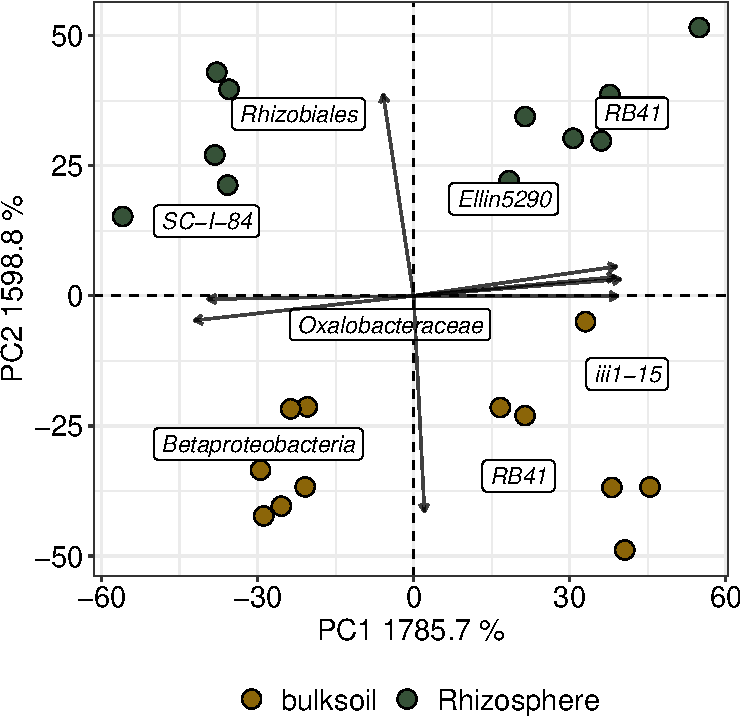
\includegraphics{Doc_pdf_files/figure-latex/unnamed-chunk-37-1} \end{center}

\begin{Shaded}
\begin{Highlighting}[]
\CommentTok{\#pdf("fig\_PCA\_flowering.pdf", width=5, height=5)}
\CommentTok{\#print(pca\_stage\_arrows\_F)}
\CommentTok{\#dev.off()}
\end{Highlighting}
\end{Shaded}

\begin{Shaded}
\begin{Highlighting}[]
\CommentTok{\# PCA GRAIN FILLING STAGE}

\NormalTok{sample\_to\_choose\_g}\OtherTok{\textless{}{-}}\NormalTok{ meta }\SpecialCharTok{\%\textgreater{}\%} \FunctionTok{filter}\NormalTok{(Stage}\SpecialCharTok{==}\StringTok{"G"}\NormalTok{)}
\NormalTok{d.pro.}\FloatTok{0.}\NormalTok{G}\OtherTok{\textless{}{-}}\NormalTok{ d.pro}\FloatTok{.0}  \SpecialCharTok{\%\textgreater{}\%}\NormalTok{ dplyr}\SpecialCharTok{::}\FunctionTok{select}\NormalTok{(}\DecValTok{0}\NormalTok{, sample\_to\_choose\_g}\SpecialCharTok{$}\NormalTok{SampleID)}
\NormalTok{d.pro.G }\OtherTok{\textless{}{-}} \FunctionTok{t}\NormalTok{(}\FunctionTok{cmultRepl}\NormalTok{(}\FunctionTok{t}\NormalTok{(d.pro.}\FloatTok{0.}\NormalTok{G), }\AttributeTok{method=}\StringTok{"CZM"}\NormalTok{, }\AttributeTok{output=}\StringTok{"p{-}counts"}\NormalTok{)) }\CommentTok{\#tratamiento de 0}

\NormalTok{d.clr.abund.codaseq.G}\OtherTok{\textless{}{-}}\FunctionTok{codaSeq.clr}\NormalTok{(}\AttributeTok{x =}\NormalTok{ d.pro.G, }\AttributeTok{samples.by.row =}\NormalTok{ F) }\CommentTok{\#transformacion clr}

\NormalTok{pcx.abund.G }\OtherTok{\textless{}{-}} \FunctionTok{prcomp}\NormalTok{(}\FunctionTok{t}\NormalTok{(d.clr.abund.codaseq.G))}



\NormalTok{PC1 }\OtherTok{\textless{}{-}} \FunctionTok{paste}\NormalTok{(}\StringTok{"PC1"}\NormalTok{, }\FunctionTok{round}\NormalTok{(}\FunctionTok{sum}\NormalTok{(pcx.abund.G}\SpecialCharTok{$}\NormalTok{sdev[}\DecValTok{1}\NormalTok{] }\SpecialCharTok{\^{}} \DecValTok{2}\NormalTok{) }\SpecialCharTok{/} \FunctionTok{mvar}\NormalTok{(d.clr.abund.codaseq.G) , }\DecValTok{1}\NormalTok{), }\StringTok{"\%"}\NormalTok{)}
\NormalTok{PC2 }\OtherTok{\textless{}{-}} \FunctionTok{paste}\NormalTok{(}\StringTok{"PC2"}\NormalTok{, }\FunctionTok{round}\NormalTok{(}\FunctionTok{sum}\NormalTok{(pcx.abund.G}\SpecialCharTok{$}\NormalTok{sdev[}\DecValTok{2}\NormalTok{] }\SpecialCharTok{\^{}} \DecValTok{2}\NormalTok{) }\SpecialCharTok{/} \FunctionTok{mvar}\NormalTok{(d.clr.abund.codaseq.G) , }\DecValTok{1}\NormalTok{), }\StringTok{"\%"}\NormalTok{)}

\NormalTok{vars\_choosing}\OtherTok{\textless{}{-}} \FunctionTok{data.frame}\NormalTok{(pcx.abund.G}\SpecialCharTok{$}\NormalTok{rotation) }\SpecialCharTok{\%\textgreater{}\%}  \FunctionTok{rownames\_to\_column}\NormalTok{(}\AttributeTok{var =} \StringTok{"FeatureID"}\NormalTok{)}\SpecialCharTok{\%\textgreater{}\%}   
  \FunctionTok{mutate}\NormalTok{(}\AttributeTok{a=}\FunctionTok{sqrt}\NormalTok{(PC1}\SpecialCharTok{\^{}}\DecValTok{2}\SpecialCharTok{+}\NormalTok{PC2}\SpecialCharTok{\^{}}\DecValTok{2}\NormalTok{)) }\SpecialCharTok{\%\textgreater{}\%}
  \FunctionTok{mutate}\NormalTok{(}\AttributeTok{PC1=}\NormalTok{PC1}\SpecialCharTok{*}\DecValTok{500}\NormalTok{, }\AttributeTok{PC2=}\NormalTok{PC2}\SpecialCharTok{*}\DecValTok{500}\NormalTok{) }\SpecialCharTok{\%\textgreater{}\%} \FunctionTok{top\_n}\NormalTok{(}\DecValTok{8}\NormalTok{, a) }\SpecialCharTok{\%\textgreater{}\%}\NormalTok{ dplyr}\SpecialCharTok{::}\FunctionTok{select}\NormalTok{(}
\NormalTok{    PC1, PC2, FeatureID) }\SpecialCharTok{\%\textgreater{}\%} \FunctionTok{right\_join}\NormalTok{(tax3, }\AttributeTok{by =} \StringTok{"FeatureID"}\NormalTok{)}

\CommentTok{\#create the base plot with only the arrows}
\NormalTok{pca\_stage\_arrows\_G}\OtherTok{\textless{}{-}} \FunctionTok{ggplot}\NormalTok{() }\SpecialCharTok{+}
  \FunctionTok{theme\_bw}\NormalTok{() }\SpecialCharTok{+}
  \FunctionTok{xlab}\NormalTok{(PC1) }\SpecialCharTok{+}
  \FunctionTok{ylab}\NormalTok{(PC2) }\SpecialCharTok{+}
  \FunctionTok{theme}\NormalTok{(}\AttributeTok{axis.text =} \FunctionTok{element\_text}\NormalTok{(}\AttributeTok{colour =} \StringTok{"black"}\NormalTok{, }\AttributeTok{size =} \DecValTok{14}\NormalTok{), }\CommentTok{\#setrting theme}
        \AttributeTok{axis.title =} \FunctionTok{element\_text}\NormalTok{(}\AttributeTok{colour =} \StringTok{"black"}\NormalTok{, }\AttributeTok{size =} \DecValTok{14}\NormalTok{),}
        \AttributeTok{legend.text =} \FunctionTok{element\_text}\NormalTok{(}\AttributeTok{size =} \DecValTok{14}\NormalTok{),}
        \AttributeTok{legend.title =} \FunctionTok{element\_blank}\NormalTok{(), }
        \AttributeTok{legend.position =} \StringTok{"bottom"}\NormalTok{, }
        \AttributeTok{legend.box =} \StringTok{"horizontal"}\NormalTok{, }
        \AttributeTok{legend.direction =} \StringTok{"horizontal"}\NormalTok{) }\SpecialCharTok{+}
  \FunctionTok{geom\_point}\NormalTok{(                              }\CommentTok{\#individuals}
    \AttributeTok{data=}\FunctionTok{data.frame}\NormalTok{(pcx.abund.G}\SpecialCharTok{$}\NormalTok{x) }\SpecialCharTok{\%\textgreater{}\%}   \FunctionTok{rownames\_to\_column}\NormalTok{(}\AttributeTok{var =} \StringTok{"SampleID"}\NormalTok{)}\SpecialCharTok{\%\textgreater{}\%}
      \FunctionTok{left\_join}\NormalTok{(meta, }\AttributeTok{by =} \StringTok{"SampleID"}\NormalTok{),}
    \FunctionTok{aes}\NormalTok{(}\AttributeTok{x=}\NormalTok{PC1, }\AttributeTok{y=}\NormalTok{PC2, }\AttributeTok{fill=}\NormalTok{Soil\_sample), }
    \AttributeTok{shape=}\DecValTok{21}\NormalTok{, }\AttributeTok{size=}\DecValTok{4}\NormalTok{) }\SpecialCharTok{+}
  \FunctionTok{geom\_vline}\NormalTok{(}\AttributeTok{xintercept =} \DecValTok{0}\NormalTok{, }\AttributeTok{linetype =} \DecValTok{2}\NormalTok{) }\SpecialCharTok{+}   \CommentTok{\#lines{-}cross}
  \FunctionTok{geom\_hline}\NormalTok{(}\AttributeTok{yintercept =} \DecValTok{0}\NormalTok{, }\AttributeTok{linetype =} \DecValTok{2}\NormalTok{) }\SpecialCharTok{+}
  \FunctionTok{scale\_fill\_manual}\NormalTok{(}\AttributeTok{values =} \FunctionTok{c}\NormalTok{(}\StringTok{"darkgoldenrod4"}\NormalTok{, }\StringTok{"\#365238"}\NormalTok{))}\SpecialCharTok{+}
\NormalTok{  ggrepel}\SpecialCharTok{::}\FunctionTok{geom\_label\_repel}\NormalTok{(}\AttributeTok{data =}\NormalTok{ vars\_choosing, }\FunctionTok{aes}\NormalTok{(}\AttributeTok{x=}\NormalTok{PC1, }\AttributeTok{y=}\NormalTok{PC2, }\AttributeTok{label=}\NormalTok{ tax),}
                            \AttributeTok{segment.colour =} \ConstantTok{NA}\NormalTok{, }\AttributeTok{box.padding =} \DecValTok{2}\NormalTok{, }\AttributeTok{fontface=}\StringTok{"italic"}\NormalTok{)}\SpecialCharTok{+}
  \FunctionTok{geom\_segment}\NormalTok{(}\AttributeTok{data =}\NormalTok{ vars\_choosing, }\FunctionTok{aes}\NormalTok{(}\AttributeTok{x =} \DecValTok{0}\NormalTok{, }\AttributeTok{y =} \DecValTok{0}\NormalTok{, }\AttributeTok{xend =}\NormalTok{ PC1, }\AttributeTok{yend =}\NormalTok{ PC2), }
               \AttributeTok{arrow=}\FunctionTok{arrow}\NormalTok{(}\AttributeTok{length=}\FunctionTok{unit}\NormalTok{(}\FloatTok{0.15}\NormalTok{,}\StringTok{"cm"}\NormalTok{)), }\CommentTok{\#arrows and names}
               \AttributeTok{alpha =} \FloatTok{0.75}\NormalTok{, }\AttributeTok{color =} \StringTok{\textquotesingle{}black\textquotesingle{}}\NormalTok{, }\AttributeTok{size=} \FloatTok{0.6}\NormalTok{)}

\NormalTok{pca\_stage\_arrows\_G}
\end{Highlighting}
\end{Shaded}

\begin{center}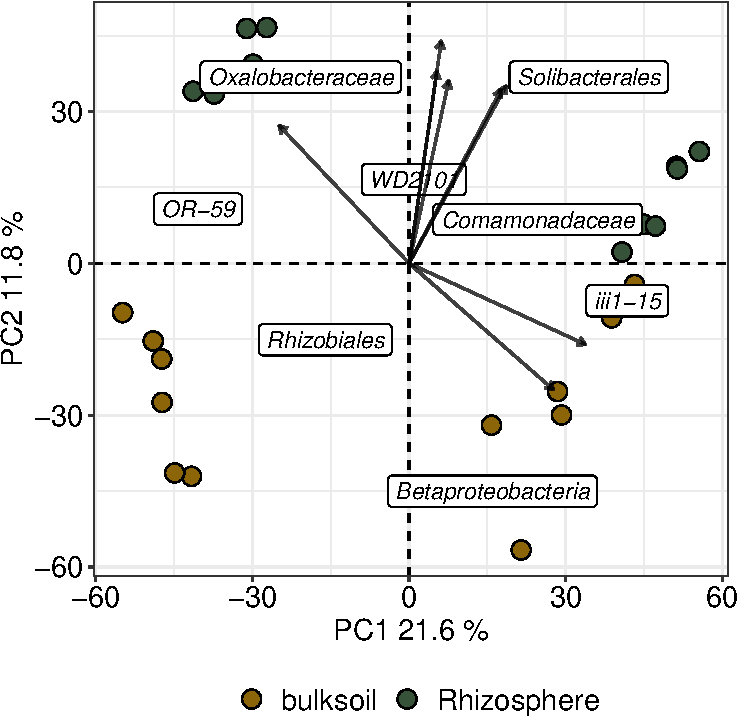
\includegraphics{Doc_pdf_files/figure-latex/unnamed-chunk-38-1} \end{center}

\begin{Shaded}
\begin{Highlighting}[]
\CommentTok{\#pdf("fig\_PCA\_grainfilling.pdf", width=5, height=5)}
\CommentTok{\#print(pca\_stage\_arrows\_G)}
\CommentTok{\#dev.off()}
\end{Highlighting}
\end{Shaded}

\hypertarget{vii.-picrust-plot}{%
\section{VII. PICRUST PLOT}\label{vii.-picrust-plot}}

\hypertarget{loading-libraries-5}{%
\subsubsection{Loading libraries}\label{loading-libraries-5}}

\begin{Shaded}
\begin{Highlighting}[]
\FunctionTok{library}\NormalTok{(ComplexHeatmap)}
\FunctionTok{library}\NormalTok{(tidyverse)}
\FunctionTok{library}\NormalTok{(circlize)}
\FunctionTok{library}\NormalTok{(viridis)}
\FunctionTok{library}\NormalTok{(RColorBrewer)}
\FunctionTok{library}\NormalTok{(cowplot)}
\end{Highlighting}
\end{Shaded}

\hypertarget{setting-common-annotations-to-heatmap}{%
\subsubsection{Setting common annotations to
heatmap}\label{setting-common-annotations-to-heatmap}}

\begin{Shaded}
\begin{Highlighting}[]
\NormalTok{levels}\OtherTok{\textless{}{-}} \FunctionTok{read\_tsv}\NormalTok{( }\StringTok{"../Data/levels.tsv"}\NormalTok{)}
\end{Highlighting}
\end{Shaded}

\begin{verbatim}
## 
## -- Column specification --------------------------------------------------------
## cols(
##   pathway = col_character(),
##   description = col_character(),
##   level1 = col_character(),
##   level2 = col_character(),
##   level3 = col_character()
## )
\end{verbatim}

\begin{Shaded}
\begin{Highlighting}[]
\NormalTok{cols\_ann }\OtherTok{\textless{}{-}} \FunctionTok{list}\NormalTok{(}\StringTok{\textquotesingle{}Superclass\textquotesingle{}} \OtherTok{=} \FunctionTok{c}\NormalTok{(}
  \StringTok{"Alcohol Degradation"}\OtherTok{=}\StringTok{"\#A6CEE3"}\NormalTok{,}
  \StringTok{"Aldehyde Degradation"}\OtherTok{=}\StringTok{"\#00FFFF"}\NormalTok{,}
  \StringTok{"Amine and Polyamine Biosynthesis"}\OtherTok{=}\StringTok{"\#B2DF8A"}\NormalTok{,}
  \StringTok{"Amine and Polyamine Degradation"}\OtherTok{=}\StringTok{"\#3300CC"}\NormalTok{,}
  \StringTok{"Amino Acid Biosynthesis"}\OtherTok{=}\StringTok{"\#33A02C"}\NormalTok{,}
  \StringTok{"Amino Acid Degradation"}\OtherTok{=}\StringTok{"\#99FFFF"}\NormalTok{,}
  \StringTok{"Aminoacyl{-}tRNA Charging"}\OtherTok{=}\StringTok{"\#99CC66"}\NormalTok{,}
  \StringTok{"Aromatic Compound Degradation"}\OtherTok{=}\StringTok{"\#006699"}\NormalTok{,}
  \StringTok{"C1 Compound Utilization and Assimilation"}\OtherTok{=}\StringTok{"\#6699CC"}\NormalTok{,}
  \StringTok{"Carbohydrate Biosynthesis"}\OtherTok{=}\StringTok{"\#B3DE69"}\NormalTok{,}
  \StringTok{"Carbohydrate Degradation"}\OtherTok{=}\StringTok{"\#6699FF"}\NormalTok{,}
  \StringTok{"Carboxylate Degradation"}\OtherTok{=}\StringTok{"\#0033CC"}\NormalTok{,}
  \StringTok{"Cell Structure Biosynthesis"}\OtherTok{=}\StringTok{"\#CCEBC5"}\NormalTok{,}
  \StringTok{"Cofactor, Carrier, and Vitamin Biosynthesis"}\OtherTok{=}\StringTok{"\#66FF00"}\NormalTok{,}
  \StringTok{"Cofactor, Prosthetic Group, Electron Carrier Degradation"}\OtherTok{=}\StringTok{"\#00CCFF"}\NormalTok{,}
  \StringTok{"Degradation/Utilization/Assimilation"}\OtherTok{=}\StringTok{"\#666699"}\NormalTok{,}
  \StringTok{"Fatty Acid and Lipid Biosynthesis"}\OtherTok{=}\StringTok{"\#66CC33"}\NormalTok{,}
  \StringTok{"Fatty Acid and Lipid Degradation"}\OtherTok{=}\StringTok{"\#000666"}\NormalTok{,}
  \StringTok{"Fermentation"}\OtherTok{=}\StringTok{"\#CC0000"}\NormalTok{,}
  \StringTok{"Glycolysis"}\OtherTok{=}\StringTok{"\#993333"}\NormalTok{,}
  \StringTok{"Inorganic Nutrient Metabolism"}\OtherTok{=}\StringTok{"\#6666FF"}\NormalTok{,}
  \StringTok{"Metabolic Regulator Biosynthesis"}\OtherTok{=}\StringTok{"\#669933"}\NormalTok{,}
  \StringTok{"Nucleic Acid Processing"}\OtherTok{=}\StringTok{"\#FFFF00"}\NormalTok{,}
  \StringTok{"Nucleoside and Nucleotide Biosynthesis"}\OtherTok{=}\StringTok{"\#339933"}\NormalTok{,}
  \StringTok{"Nucleoside and Nucleotide Degradation"}\OtherTok{=}\StringTok{"\#99CCFF"}\NormalTok{,}
  \StringTok{"Other"}\OtherTok{=}\StringTok{"\#000000"}\NormalTok{,}
  \StringTok{"Other Biosynthesis"}\OtherTok{=}\StringTok{"\#069966"}\NormalTok{,}
  \StringTok{"Pentose Phosphate Pathways"}\OtherTok{=}\StringTok{"\#FF6666"}\NormalTok{,}
  \StringTok{"Polyprenyl Biosynthesis"}\OtherTok{=}\StringTok{"\#00FF33"}\NormalTok{,}
  \StringTok{"Respiration"}\OtherTok{=}\StringTok{"\#CC6666"}\NormalTok{,}
  \StringTok{"Secondary Metabolite Biosynthesis"}\OtherTok{=}\StringTok{"\#99CC00"}\NormalTok{,}
  \StringTok{"Secondary Metabolite Degradation"}\OtherTok{=}\StringTok{"\#66CCCC"}\NormalTok{,}
  \StringTok{"TCA cycle"}\OtherTok{=}\StringTok{"\#990033"}\NormalTok{,}
  \StringTok{"Tetrapyrrole Biosynthesis"}\OtherTok{=}\StringTok{"\#CCFF99"}\NormalTok{))}

\NormalTok{cols\_pvalue }\OtherTok{\textless{}{-}} \FunctionTok{list}\NormalTok{(}\StringTok{\textquotesingle{}p{-}value\textquotesingle{}} \OtherTok{=} \FunctionTok{c}\NormalTok{(}\StringTok{"\textless{}0.001"} \OtherTok{=} \StringTok{\textquotesingle{}\#AB0000\textquotesingle{}}\NormalTok{,}
                                  \StringTok{"\textless{}0.01"} \OtherTok{=} \StringTok{\textquotesingle{}\#FF0000\textquotesingle{}}\NormalTok{,}
                                  \StringTok{"\textless{}0.05"}\OtherTok{=}\StringTok{"\#FFB6B6"}\NormalTok{))}

\NormalTok{effect\_col\_fun }\OtherTok{=}\FunctionTok{colorRamp2}\NormalTok{(}\FunctionTok{c}\NormalTok{(}\SpecialCharTok{{-}}\FloatTok{1.5}\NormalTok{, }\DecValTok{0}\NormalTok{, }\FloatTok{1.5}\NormalTok{), }\FunctionTok{c}\NormalTok{(}
  \StringTok{"lightsalmon4"}\NormalTok{, }\StringTok{"white"}\NormalTok{, }\StringTok{"lightseagreen"}\NormalTok{))}
\end{Highlighting}
\end{Shaded}

\hypertarget{treatment-picrust}{%
\subsubsection{Treatment Picrust}\label{treatment-picrust}}

\begin{Shaded}
\begin{Highlighting}[]
\NormalTok{aldex\_all\_dif}\OtherTok{\textless{}{-}} \FunctionTok{read\_tsv}\NormalTok{( }\StringTok{"../Data/aldex\_Treatment\_picrust.tsv"}\NormalTok{)}

\NormalTok{annotation\_heatmap}\OtherTok{\textless{}{-}}\NormalTok{ aldex\_all\_dif}\SpecialCharTok{\%\textgreater{}\%} \FunctionTok{left\_join}\NormalTok{(}
\NormalTok{  levels, }\AttributeTok{by =} \FunctionTok{c}\NormalTok{(}\StringTok{"Feature.ID"}\OtherTok{=}\StringTok{"pathway"}\NormalTok{))}\SpecialCharTok{\%\textgreater{}\%}\NormalTok{ dplyr}\SpecialCharTok{::}\FunctionTok{select}\NormalTok{(}
\NormalTok{  level2, Feature.ID, p.Value, effect, diff.btw) }\SpecialCharTok{\%\textgreater{}\%} \FunctionTok{mutate\_at}\NormalTok{(}\FunctionTok{c}\NormalTok{(}
    \DecValTok{3}\NormalTok{), }\FunctionTok{funs}\NormalTok{(}\AttributeTok{p.value =} \FunctionTok{case\_when}\NormalTok{(}
\NormalTok{    . }\SpecialCharTok{\textless{}=} \FloatTok{0.001} \SpecialCharTok{\textasciitilde{}} \StringTok{"\textless{}0.001"}\NormalTok{,}
\NormalTok{    . }\SpecialCharTok{\textgreater{}}  \FloatTok{0.001} \SpecialCharTok{\&}\NormalTok{ .  }\SpecialCharTok{\textless{}=} \FloatTok{0.01} \SpecialCharTok{\textasciitilde{}} \StringTok{"\textless{}0.01"}\NormalTok{,}
\NormalTok{    . }\SpecialCharTok{\textgreater{}}  \FloatTok{0.01} \SpecialCharTok{\&}\NormalTok{ .  }\SpecialCharTok{\textless{}=} \FloatTok{0.05} \SpecialCharTok{\textasciitilde{}} \StringTok{"\textless{}0.05"}\NormalTok{)))}\SpecialCharTok{\%\textgreater{}\%}\FunctionTok{arrange}\NormalTok{(}
\NormalTok{      diff.btw)}\SpecialCharTok{\%\textgreater{}\%}\FunctionTok{column\_to\_rownames}\NormalTok{(}\AttributeTok{var =} \StringTok{"Feature.ID"}\NormalTok{)}

\NormalTok{data\_heatmap}\OtherTok{\textless{}{-}}\NormalTok{ aldex\_all\_dif }\SpecialCharTok{\%\textgreater{}\%} \FunctionTok{arrange}\NormalTok{(diff.btw)}\SpecialCharTok{\%\textgreater{}\%}\FunctionTok{column\_to\_rownames}\NormalTok{(}
  \AttributeTok{var =} \StringTok{"Feature.ID"}\NormalTok{)}\SpecialCharTok{\%\textgreater{}\%}\NormalTok{dplyr}\SpecialCharTok{::}\FunctionTok{select}\NormalTok{(}
\NormalTok{    rab.win.CA, rab.win.CP, diff.btw) }\SpecialCharTok{\%\textgreater{}\%} \FunctionTok{arrange}\NormalTok{(diff.btw)}

\NormalTok{color\_heatmap}\OtherTok{=} \FunctionTok{colorRamp2}\NormalTok{(}\FunctionTok{seq}\NormalTok{(}\FunctionTok{min}\NormalTok{(data\_heatmap), }\FunctionTok{max}\NormalTok{(data\_heatmap), }\AttributeTok{length =} \DecValTok{5}\NormalTok{), }\FunctionTok{c}\NormalTok{(}
  \StringTok{"\#0000FF"}\NormalTok{,}\StringTok{"\#5499C7"}\NormalTok{, }\StringTok{"\#DAE7E4"}\NormalTok{,  }\StringTok{"red"}\NormalTok{, }\StringTok{"\#FF0000"}\NormalTok{))}

\NormalTok{colAnn }\OtherTok{\textless{}{-}} \FunctionTok{HeatmapAnnotation}\NormalTok{(}\AttributeTok{Superclass =}\NormalTok{ annotation\_heatmap}\SpecialCharTok{$}\NormalTok{level2,}
                            \AttributeTok{which =} \StringTok{\textquotesingle{}row\textquotesingle{}}\NormalTok{,}
                            \AttributeTok{col =}\NormalTok{ cols\_ann,}
                            \AttributeTok{show\_legend =}\NormalTok{ F)}

\NormalTok{annP2 }\OtherTok{=} \FunctionTok{HeatmapAnnotation}\NormalTok{(}\StringTok{"p{-}value"} \OtherTok{=}\NormalTok{ annotation\_heatmap}\SpecialCharTok{$}\NormalTok{p.value,}
                          \AttributeTok{which =} \StringTok{"row"}\NormalTok{, }\AttributeTok{col =}\NormalTok{ cols\_pvalue,}
                          \AttributeTok{show\_legend =}\NormalTok{ F)}

\NormalTok{annEffect }\OtherTok{=} \FunctionTok{HeatmapAnnotation}\NormalTok{(}\StringTok{"effect{-}size"} \OtherTok{=}\NormalTok{ annotation\_heatmap}\SpecialCharTok{$}\NormalTok{effect,}
                              \AttributeTok{which =} \StringTok{"row"}\NormalTok{, }\AttributeTok{col =} \FunctionTok{list}\NormalTok{(}
                              \StringTok{"effect{-}size"} \OtherTok{=}\NormalTok{ effect\_col\_fun),}
                              \AttributeTok{show\_legend =}\NormalTok{ F, }
                              \AttributeTok{gp =} \FunctionTok{gpar}\NormalTok{(}\AttributeTok{col =} \StringTok{"white"}\NormalTok{))}

\NormalTok{bardif}\OtherTok{=} \FunctionTok{rowAnnotation}\NormalTok{(}
  \StringTok{"difference between groups"} \OtherTok{=} \FunctionTok{anno\_barplot}\NormalTok{(}
\NormalTok{    annotation\_heatmap}\SpecialCharTok{$}\NormalTok{diff.btw, }\AttributeTok{width =} \FunctionTok{unit}\NormalTok{(}\DecValTok{4}\NormalTok{, }\StringTok{"cm"}\NormalTok{)))}



\NormalTok{ht5}\OtherTok{\textless{}{-}}\NormalTok{ComplexHeatmap}\SpecialCharTok{::}\FunctionTok{Heatmap}\NormalTok{(}
\NormalTok{  data\_heatmap[}\SpecialCharTok{{-}}\DecValTok{3}\NormalTok{],  }
  \AttributeTok{row\_dend\_reorder =}\NormalTok{ F, }\AttributeTok{col =}\NormalTok{ color\_heatmap,}
  \AttributeTok{width =} \FunctionTok{ncol}\NormalTok{(data\_heatmap)}\SpecialCharTok{*}\FunctionTok{unit}\NormalTok{(}\FloatTok{0.6}\NormalTok{, }\StringTok{"cm"}\NormalTok{),}
  \AttributeTok{height =} \FunctionTok{ncol}\NormalTok{(data\_heatmap)}\SpecialCharTok{*}\FunctionTok{unit}\NormalTok{(}\DecValTok{8}\NormalTok{, }\StringTok{"cm"}\NormalTok{),}
  \AttributeTok{left\_annotation =}  \FunctionTok{c}\NormalTok{(annP2, annEffect, colAnn),}
  \AttributeTok{heatmap\_legend\_param =} \FunctionTok{list}\NormalTok{(}\AttributeTok{direction =} \StringTok{"vertical"}\NormalTok{ ),}
  \AttributeTok{right\_annotation =} \FunctionTok{c}\NormalTok{(bardif),}
  \AttributeTok{cluster\_column\_slices =} \ConstantTok{FALSE}\NormalTok{,}
  \AttributeTok{column\_split =} \FunctionTok{rep}\NormalTok{(}\FunctionTok{c}\NormalTok{(}\StringTok{"CA"}\NormalTok{, }\StringTok{"CP"}\NormalTok{)),}
  \AttributeTok{cluster\_rows =}\NormalTok{ F,}
  \AttributeTok{column\_km =} \DecValTok{1}\NormalTok{, }\AttributeTok{column\_title\_gp =} \FunctionTok{gpar}\NormalTok{(}
  \AttributeTok{fill =} \FunctionTok{c}\NormalTok{(}\StringTok{"\#212F3D"}\NormalTok{, }\StringTok{"\#839192"}\NormalTok{ ), }\AttributeTok{col=}\StringTok{"white"}\NormalTok{),}
  \AttributeTok{border =}\NormalTok{ F, }\AttributeTok{column\_gap =} \FunctionTok{unit}\NormalTok{(}\FloatTok{0.5}\NormalTok{, }\StringTok{"mm"}\NormalTok{), }
  \AttributeTok{row\_dend\_side =} \StringTok{"left"}\NormalTok{,}\AttributeTok{row\_names\_side =} \StringTok{"right"}\NormalTok{,}\AttributeTok{show\_row\_names =}\NormalTok{ F ,}
  \AttributeTok{rect\_gp =} \FunctionTok{gpar}\NormalTok{(}\AttributeTok{col =} \StringTok{"white"}\NormalTok{, }\AttributeTok{lwd =} \FloatTok{0.2}\NormalTok{), }\AttributeTok{row\_names\_gp =} \FunctionTok{gpar}\NormalTok{(}
  \AttributeTok{fontface =}\StringTok{"italic"}\NormalTok{, }\AttributeTok{fontsize=}\DecValTok{10}\NormalTok{),}
  \AttributeTok{cluster\_columns =}\NormalTok{ F,}
  \AttributeTok{show\_column\_names =}\NormalTok{ F, }\AttributeTok{name =} \StringTok{"rab.Win"}\NormalTok{)}

\CommentTok{\#ht5}

\NormalTok{ht5}\FloatTok{.2}\OtherTok{\textless{}{-}}\FunctionTok{draw}\NormalTok{(ht5, }\AttributeTok{heatmap\_legend\_side =} \StringTok{"bottom"}\NormalTok{)}
\end{Highlighting}
\end{Shaded}

\begin{center}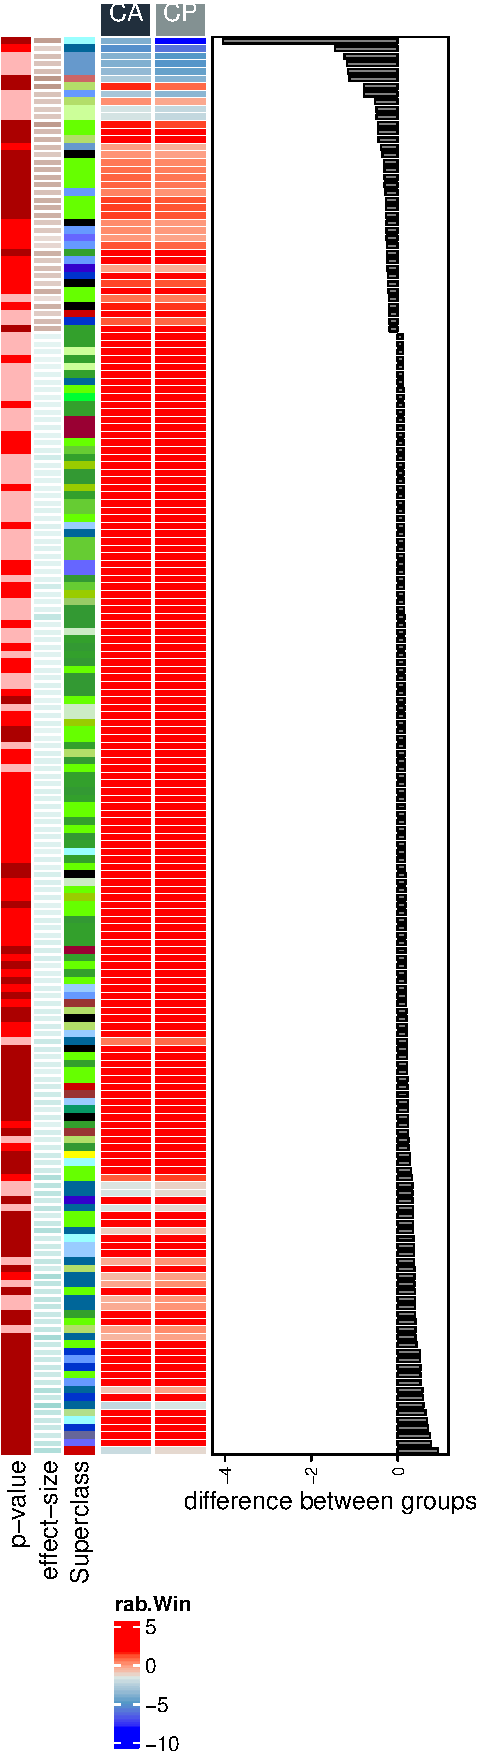
\includegraphics{Doc_pdf_files/figure-latex/unnamed-chunk-41-1} \end{center}

\begin{Shaded}
\begin{Highlighting}[]
\CommentTok{\#pdf("fig\_picrust\_TREATMENT2.pdf", width=7, height=20)}
\CommentTok{\#print(ht5.2)}
\CommentTok{\#dev.off()}

\CommentTok{\#pdf("fig\_picrust\_TREATMENT.pdf", width=10, height=10)}
\CommentTok{\#print(ht5)}
\CommentTok{\#dev.off()}
\end{Highlighting}
\end{Shaded}

\hypertarget{soil-picrust}{%
\subsubsection{Soil Picrust}\label{soil-picrust}}

\begin{Shaded}
\begin{Highlighting}[]
\NormalTok{aldex\_all\_dif}\OtherTok{\textless{}{-}} \FunctionTok{read\_tsv}\NormalTok{( }\StringTok{"../Data/aldex\_Soil\_picrust.tsv"}\NormalTok{)}

\NormalTok{annotation\_heatmap}\OtherTok{\textless{}{-}}\NormalTok{ aldex\_all\_dif}\SpecialCharTok{\%\textgreater{}\%} \FunctionTok{left\_join}\NormalTok{(levels, }\AttributeTok{by =} \FunctionTok{c}\NormalTok{(}
  \StringTok{"Feature.ID"}\OtherTok{=}\StringTok{"pathway"}\NormalTok{))}\SpecialCharTok{\%\textgreater{}\%}\NormalTok{ dplyr}\SpecialCharTok{::}\FunctionTok{select}\NormalTok{(}
\NormalTok{  level2, Feature.ID, p.Value, effect, diff.btw, rab.win.Rh, rab.win.Bs )}\SpecialCharTok{\%\textgreater{}\%} \FunctionTok{mutate\_at}\NormalTok{(}
    \FunctionTok{c}\NormalTok{(}\DecValTok{3}\NormalTok{), }\FunctionTok{funs}\NormalTok{(}\AttributeTok{p.value =} \FunctionTok{case\_when}\NormalTok{(}
\NormalTok{    . }\SpecialCharTok{\textless{}=} \FloatTok{0.001} \SpecialCharTok{\textasciitilde{}} \StringTok{"\textless{}0.001"}\NormalTok{,}
\NormalTok{    . }\SpecialCharTok{\textgreater{}}  \FloatTok{0.001} \SpecialCharTok{\&}\NormalTok{ .  }\SpecialCharTok{\textless{}=} \FloatTok{0.01} \SpecialCharTok{\textasciitilde{}} \StringTok{"\textless{}0.01"}\NormalTok{,}
\NormalTok{    . }\SpecialCharTok{\textgreater{}}  \FloatTok{0.01} \SpecialCharTok{\&}\NormalTok{ .  }\SpecialCharTok{\textless{}=} \FloatTok{0.05} \SpecialCharTok{\textasciitilde{}} \StringTok{"\textless{}0.05"}\NormalTok{)))}\SpecialCharTok{\%\textgreater{}\%} \FunctionTok{mutate}\NormalTok{(}
      \AttributeTok{diff.btw2 =}\NormalTok{ diff.btw}\SpecialCharTok{*{-}}\DecValTok{1}\NormalTok{, }\AttributeTok{effect2 =}\NormalTok{ effect}\SpecialCharTok{*{-}}\DecValTok{1}\NormalTok{ ) }\SpecialCharTok{\%\textgreater{}\%} \FunctionTok{arrange}\NormalTok{(}
\NormalTok{      diff.btw2)}\SpecialCharTok{\%\textgreater{}\%}\FunctionTok{column\_to\_rownames}\NormalTok{(}\AttributeTok{var =} \StringTok{"Feature.ID"}\NormalTok{)}

\NormalTok{data\_heatmap}\OtherTok{\textless{}{-}}\NormalTok{ annotation\_heatmap}\SpecialCharTok{\%\textgreater{}\%}\NormalTok{dplyr}\SpecialCharTok{::}\FunctionTok{select}\NormalTok{(}
\NormalTok{  rab.win.Bs, rab.win.Rh, diff.btw2 ) }\SpecialCharTok{\%\textgreater{}\%} \FunctionTok{arrange}\NormalTok{(}
\NormalTok{    diff.btw2)}

\NormalTok{color\_heatmap}\OtherTok{=} \FunctionTok{colorRamp2}\NormalTok{(}
  \FunctionTok{seq}\NormalTok{(}\FunctionTok{min}\NormalTok{(data\_heatmap), }\FunctionTok{max}\NormalTok{(data\_heatmap), }
  \AttributeTok{length =} \DecValTok{5}\NormalTok{), }\FunctionTok{c}\NormalTok{(}\StringTok{"\#0000FF"}\NormalTok{,}\StringTok{"\#5499C7"}\NormalTok{, }\StringTok{"\#DAE7E4"}\NormalTok{,  }\StringTok{"red"}\NormalTok{, }\StringTok{"\#FF0000"}\NormalTok{))}


\NormalTok{colAnn }\OtherTok{\textless{}{-}} \FunctionTok{HeatmapAnnotation}\NormalTok{(}\AttributeTok{Superclass =}\NormalTok{ annotation\_heatmap}\SpecialCharTok{$}\NormalTok{level2,}
                            \AttributeTok{which =} \StringTok{\textquotesingle{}row\textquotesingle{}}\NormalTok{,}
                            \AttributeTok{col =}\NormalTok{ cols\_ann,}
                            \AttributeTok{show\_legend =}\NormalTok{ F)}

\NormalTok{annP2 }\OtherTok{=} \FunctionTok{HeatmapAnnotation}\NormalTok{(}\StringTok{"p{-}value"} \OtherTok{=}\NormalTok{ annotation\_heatmap}\SpecialCharTok{$}\NormalTok{p.value,}
                          \AttributeTok{which =} \StringTok{"row"}\NormalTok{, }\AttributeTok{col =}\NormalTok{ cols\_pvalue,}
                          \AttributeTok{show\_legend =}\NormalTok{ F)}

\NormalTok{annEffect }\OtherTok{=} \FunctionTok{HeatmapAnnotation}\NormalTok{(}\StringTok{"effect{-}size"} \OtherTok{=}\NormalTok{ annotation\_heatmap}\SpecialCharTok{$}\NormalTok{effect,}
                              \AttributeTok{which =} \StringTok{"row"}\NormalTok{, }\AttributeTok{col =} \FunctionTok{list}\NormalTok{(}
                              \StringTok{"effect{-}size"} \OtherTok{=}\NormalTok{ effect\_col\_fun),}
                              \AttributeTok{show\_legend =}\NormalTok{ F, }
                              \AttributeTok{gp =} \FunctionTok{gpar}\NormalTok{(}\AttributeTok{col =} \StringTok{"white"}\NormalTok{))}

\NormalTok{bardif}\OtherTok{=} \FunctionTok{rowAnnotation}\NormalTok{(}
  \StringTok{"difference between groups"} \OtherTok{=} \FunctionTok{anno\_barplot}\NormalTok{(}
\NormalTok{    annotation\_heatmap}\SpecialCharTok{$}\NormalTok{diff.btw, }\AttributeTok{width =} \FunctionTok{unit}\NormalTok{(}\DecValTok{4}\NormalTok{, }\StringTok{"cm"}\NormalTok{)))}




\NormalTok{ht4}\OtherTok{\textless{}{-}}\NormalTok{ComplexHeatmap}\SpecialCharTok{::}\FunctionTok{Heatmap}\NormalTok{(}
\NormalTok{  data\_heatmap[}\SpecialCharTok{{-}}\DecValTok{3}\NormalTok{],  }\AttributeTok{row\_dend\_reorder =}\NormalTok{ F, }\AttributeTok{col =}\NormalTok{ color\_heatmap,}
  \AttributeTok{width =} \FunctionTok{ncol}\NormalTok{(data\_heatmap)}\SpecialCharTok{*}\FunctionTok{unit}\NormalTok{(}\FloatTok{0.6}\NormalTok{, }\StringTok{"cm"}\NormalTok{),}
  \AttributeTok{height =} \FunctionTok{ncol}\NormalTok{(data\_heatmap)}\SpecialCharTok{*}\FunctionTok{unit}\NormalTok{(}\DecValTok{8}\NormalTok{, }\StringTok{"cm"}\NormalTok{),}
  \AttributeTok{left\_annotation =}  \FunctionTok{c}\NormalTok{(annP2, annEffect, colAnn),}
  \AttributeTok{heatmap\_legend\_param =} \FunctionTok{list}\NormalTok{(}\AttributeTok{direction =} \StringTok{"vertical"}\NormalTok{ ),}
  \AttributeTok{right\_annotation =} \FunctionTok{c}\NormalTok{(bardif),}
  \AttributeTok{cluster\_column\_slices =} \ConstantTok{FALSE}\NormalTok{,}
  \AttributeTok{column\_split =} \FunctionTok{rep}\NormalTok{(}\FunctionTok{c}\NormalTok{(}\StringTok{"BS"}\NormalTok{, }\StringTok{"Rh"}\NormalTok{)),}
  \AttributeTok{show\_heatmap\_legend =}\NormalTok{ T,}
  \AttributeTok{cluster\_rows =}\NormalTok{ F,}
  \AttributeTok{column\_km =} \DecValTok{1}\NormalTok{, }\AttributeTok{column\_title\_gp =} \FunctionTok{gpar}\NormalTok{(}
  \AttributeTok{fill =} \FunctionTok{c}\NormalTok{(}\StringTok{"darkgoldenrod4"}\NormalTok{, }\StringTok{"\#365238"}\NormalTok{ ), }\AttributeTok{col=}\StringTok{"white"}\NormalTok{),}
  \AttributeTok{border =}\NormalTok{ F, }\AttributeTok{column\_gap =} \FunctionTok{unit}\NormalTok{(}\FloatTok{0.5}\NormalTok{, }\StringTok{"mm"}\NormalTok{),}
  \AttributeTok{row\_dend\_side =} \StringTok{"left"}\NormalTok{,}\AttributeTok{row\_names\_side =} \StringTok{"right"}\NormalTok{,}\AttributeTok{show\_row\_names =}\NormalTok{ F ,}
  \AttributeTok{rect\_gp =} \FunctionTok{gpar}\NormalTok{(}\AttributeTok{col =} \StringTok{"white"}\NormalTok{, }\AttributeTok{lwd =} \FloatTok{0.2}\NormalTok{), }\AttributeTok{row\_names\_gp =} \FunctionTok{gpar}\NormalTok{(}
  \AttributeTok{fontface =}\StringTok{"italic"}\NormalTok{, }\AttributeTok{fontsize=}\DecValTok{10}\NormalTok{),}
  \AttributeTok{cluster\_columns =}\NormalTok{ F,}
  \AttributeTok{show\_column\_names =}\NormalTok{ F, }\AttributeTok{name =} \StringTok{"rab.Win"}\NormalTok{)}

\NormalTok{ht4}\FloatTok{.2}\OtherTok{\textless{}{-}}\FunctionTok{draw}\NormalTok{(ht4, }\AttributeTok{heatmap\_legend\_side =} \StringTok{"bottom"}\NormalTok{)}
\end{Highlighting}
\end{Shaded}

\begin{center}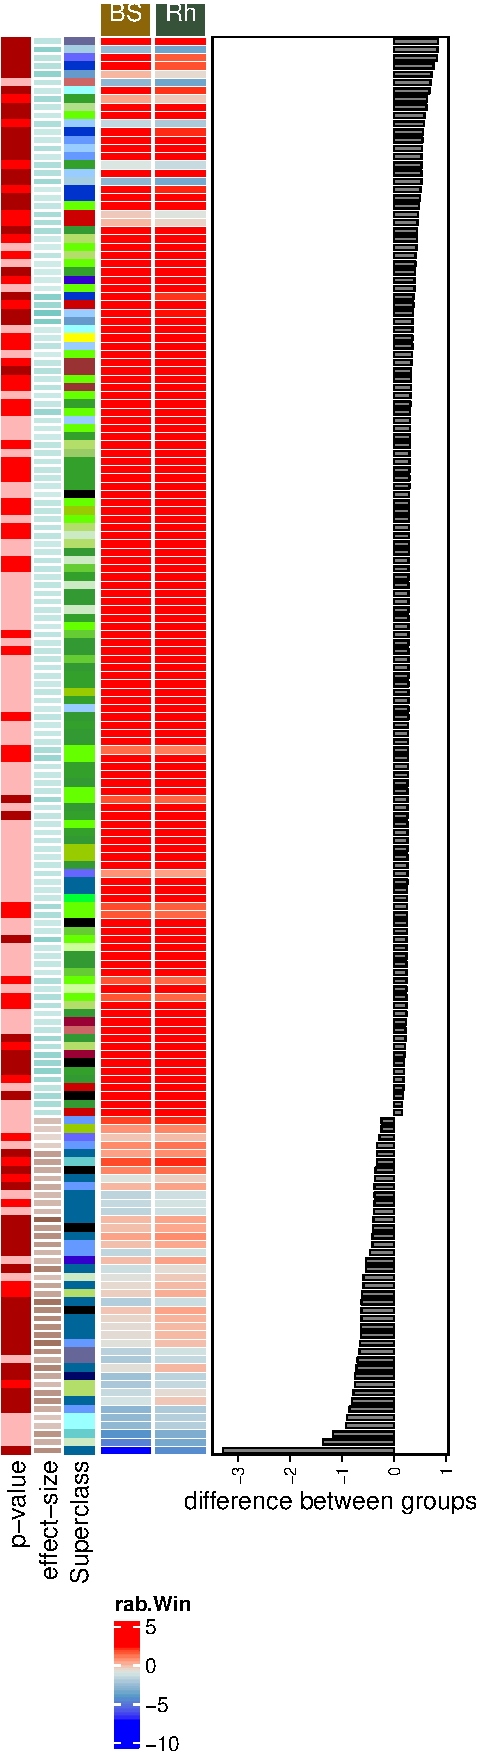
\includegraphics{Doc_pdf_files/figure-latex/unnamed-chunk-42-1} \end{center}

\begin{Shaded}
\begin{Highlighting}[]
\CommentTok{\#pdf("fig\_picrust\_soil2.pdf", width=7, height=20)}
\CommentTok{\#print(ht4.2)}
\CommentTok{\#dev.off()}

\CommentTok{\#pdf("fig\_picrust\_soil.pdf", width=10, height=10)}
\CommentTok{\#print(ht4)}
\CommentTok{\#dev.off()}
\end{Highlighting}
\end{Shaded}

\hypertarget{stage-picrust}{%
\subsubsection{Stage Picrust}\label{stage-picrust}}

\hypertarget{vegetative-vs-flowering}{%
\paragraph{Vegetative vs Flowering}\label{vegetative-vs-flowering}}

\begin{Shaded}
\begin{Highlighting}[]
\CommentTok{\# VvsF}
\NormalTok{aldex\_all\_dif}\OtherTok{\textless{}{-}} \FunctionTok{read\_tsv}\NormalTok{( }\StringTok{"../Data/aldex\_Stage\_vvsf\_picrust.tsv"}\NormalTok{)}


\CommentTok{\#contruct heatmap}
\NormalTok{annotation\_heatmap}\OtherTok{\textless{}{-}}\NormalTok{ aldex\_all\_dif}\SpecialCharTok{\%\textgreater{}\%} \FunctionTok{left\_join}\NormalTok{(}
\NormalTok{  levels, }\AttributeTok{by =} \FunctionTok{c}\NormalTok{(}\StringTok{"Feature.ID"}\OtherTok{=}\StringTok{"pathway"}\NormalTok{))}\SpecialCharTok{\%\textgreater{}\%}\NormalTok{ dplyr}\SpecialCharTok{::}\FunctionTok{select}\NormalTok{(}
\NormalTok{  level2, Feature.ID, p.Value, effect, diff.btw) }\SpecialCharTok{\%\textgreater{}\%} \FunctionTok{mutate\_at}\NormalTok{(}\FunctionTok{c}\NormalTok{(}\DecValTok{3}\NormalTok{), }\FunctionTok{funs}\NormalTok{(}
    \AttributeTok{p.value =} \FunctionTok{case\_when}\NormalTok{(}
\NormalTok{    . }\SpecialCharTok{\textless{}=} \FloatTok{0.001} \SpecialCharTok{\textasciitilde{}} \StringTok{"\textless{}0.001"}\NormalTok{,}
\NormalTok{    . }\SpecialCharTok{\textgreater{}}  \FloatTok{0.001} \SpecialCharTok{\&}\NormalTok{ .  }\SpecialCharTok{\textless{}=} \FloatTok{0.01} \SpecialCharTok{\textasciitilde{}} \StringTok{"\textless{}0.01"}\NormalTok{,}
\NormalTok{    . }\SpecialCharTok{\textgreater{}}  \FloatTok{0.01} \SpecialCharTok{\&}\NormalTok{ .  }\SpecialCharTok{\textless{}=} \FloatTok{0.05} \SpecialCharTok{\textasciitilde{}} \StringTok{"\textless{}0.05"}\NormalTok{)))}\SpecialCharTok{\%\textgreater{}\%}\FunctionTok{arrange}\NormalTok{(}
\NormalTok{      diff.btw)}\SpecialCharTok{\%\textgreater{}\%}\FunctionTok{column\_to\_rownames}\NormalTok{(}\AttributeTok{var =} \StringTok{"Feature.ID"}\NormalTok{)}

\NormalTok{data\_heatmap}\OtherTok{\textless{}{-}}\NormalTok{ aldex\_all\_dif }\SpecialCharTok{\%\textgreater{}\%} \FunctionTok{arrange}\NormalTok{(}
\NormalTok{  diff.btw)}\SpecialCharTok{\%\textgreater{}\%}\FunctionTok{column\_to\_rownames}\NormalTok{(}
\AttributeTok{var =} \StringTok{"Feature.ID"}\NormalTok{)}\SpecialCharTok{\%\textgreater{}\%}\NormalTok{dplyr}\SpecialCharTok{::}\FunctionTok{select}\NormalTok{(}
\NormalTok{  rab.win}\FloatTok{.0}\NormalTok{, rab.win}\FloatTok{.1}\NormalTok{, diff.btw) }\SpecialCharTok{\%\textgreater{}\%} \FunctionTok{rename}\NormalTok{(}
  \AttributeTok{Ve=}\NormalTok{rab.win}\FloatTok{.0}\NormalTok{ , }\AttributeTok{Fl=}\NormalTok{rab.win}\FloatTok{.1}\NormalTok{) }\SpecialCharTok{\%\textgreater{}\%} \FunctionTok{arrange}\NormalTok{(diff.btw)}

\NormalTok{colAnn }\OtherTok{\textless{}{-}} \FunctionTok{HeatmapAnnotation}\NormalTok{(}
  \AttributeTok{Superclass =}\NormalTok{ annotation\_heatmap}\SpecialCharTok{$}\NormalTok{level2,}
                            \AttributeTok{which =} \StringTok{\textquotesingle{}row\textquotesingle{}}\NormalTok{,}
                            \AttributeTok{col =}\NormalTok{ cols\_ann,}
                            \AttributeTok{show\_legend =}\NormalTok{ F)}


\NormalTok{annP2 }\OtherTok{=} \FunctionTok{HeatmapAnnotation}\NormalTok{(}\StringTok{"p{-}value"} \OtherTok{=}\NormalTok{ annotation\_heatmap}\SpecialCharTok{$}\NormalTok{p.value,}
                          \AttributeTok{which =} \StringTok{"row"}\NormalTok{, }\AttributeTok{col =}\NormalTok{ cols\_pvalue,}
                          \AttributeTok{show\_legend =}\NormalTok{ F)}


\CommentTok{\#effect annotation}

\NormalTok{annEffect }\OtherTok{=} \FunctionTok{HeatmapAnnotation}\NormalTok{(}
  \StringTok{"effect{-}size"} \OtherTok{=}\NormalTok{ annotation\_heatmap}\SpecialCharTok{$}\NormalTok{effect,}
   \AttributeTok{which =} \StringTok{"row"}\NormalTok{, }\AttributeTok{col =} \FunctionTok{list}\NormalTok{(}\StringTok{"effect{-}size"} \OtherTok{=}\NormalTok{ effect\_col\_fun),}
   \AttributeTok{show\_legend  =}\NormalTok{F, }
   \AttributeTok{gp =} \FunctionTok{gpar}\NormalTok{(}\AttributeTok{col =} \StringTok{"white"}\NormalTok{))}

\CommentTok{\#barplot annotation}
\NormalTok{bardif}\OtherTok{=} \FunctionTok{rowAnnotation}\NormalTok{(}
  \StringTok{"difference between groups"} \OtherTok{=} \FunctionTok{anno\_barplot}\NormalTok{(}
\NormalTok{    annotation\_heatmap}\SpecialCharTok{$}\NormalTok{diff.btw, }\AttributeTok{width =} \FunctionTok{unit}\NormalTok{(}\DecValTok{4}\NormalTok{, }\StringTok{"cm"}\NormalTok{)))}



\NormalTok{color\_heatmap}\OtherTok{=} \FunctionTok{colorRamp2}\NormalTok{(}
  \FunctionTok{seq}\NormalTok{(}\FunctionTok{min}\NormalTok{(data\_heatmap), }\FunctionTok{max}\NormalTok{(}
\NormalTok{    data\_heatmap), }\AttributeTok{length =} \DecValTok{5}\NormalTok{), }\FunctionTok{c}\NormalTok{(}
      \StringTok{"\#0000FF"}\NormalTok{,}\StringTok{"\#5499C7"}\NormalTok{, }\StringTok{"\#DAE7E4"}\NormalTok{,  }\StringTok{"red"}\NormalTok{, }\StringTok{"\#FF0000"}\NormalTok{))}

\NormalTok{htVvsF}\OtherTok{\textless{}{-}}\NormalTok{  ComplexHeatmap}\SpecialCharTok{::}\FunctionTok{Heatmap}\NormalTok{(}
  \FunctionTok{as.matrix}\NormalTok{(data\_heatmap[}\SpecialCharTok{{-}}\DecValTok{3}\NormalTok{]), }\AttributeTok{col =}\NormalTok{ color\_heatmap, }\AttributeTok{row\_dend\_reorder =}\NormalTok{ F, }
  \AttributeTok{width =} \FunctionTok{ncol}\NormalTok{(data\_heatmap)}\SpecialCharTok{*}\FunctionTok{unit}\NormalTok{(}\FloatTok{0.6}\NormalTok{, }\StringTok{"cm"}\NormalTok{),}
  \AttributeTok{height =} \FunctionTok{ncol}\NormalTok{(data\_heatmap)}\SpecialCharTok{*}\FunctionTok{unit}\NormalTok{(}\DecValTok{10}\NormalTok{, }\StringTok{"cm"}\NormalTok{),}
  \AttributeTok{left\_annotation =}  \FunctionTok{c}\NormalTok{(annP2,annEffect, colAnn),}
  \AttributeTok{heatmap\_legend\_param =} \FunctionTok{list}\NormalTok{(}\AttributeTok{direction =} \StringTok{"vertical"}\NormalTok{ ),}
  \AttributeTok{right\_annotation =} \FunctionTok{c}\NormalTok{(bardif),}
  \AttributeTok{column\_split =} \FunctionTok{factor}\NormalTok{(}\FunctionTok{rep}\NormalTok{(}\FunctionTok{c}\NormalTok{(}\StringTok{"V"}\NormalTok{, }\StringTok{"F"}\NormalTok{)), }\AttributeTok{levels =} \FunctionTok{c}\NormalTok{(}\StringTok{"V"}\NormalTok{, }\StringTok{"F"}\NormalTok{)),}
  \AttributeTok{cluster\_rows =}\NormalTok{ F,}
  \AttributeTok{column\_km =} \DecValTok{1}\NormalTok{, }
  \AttributeTok{column\_title\_gp =} \FunctionTok{gpar}\NormalTok{(}\AttributeTok{fill =} \FunctionTok{c}\NormalTok{(}
  \StringTok{"darkolivegreen1"}\NormalTok{,}\StringTok{"darkolivegreen3"}\NormalTok{), }\AttributeTok{col=}\StringTok{"white"}\NormalTok{),}
   \AttributeTok{border =}\NormalTok{ F, }\AttributeTok{column\_gap =} \FunctionTok{unit}\NormalTok{(}\FloatTok{0.5}\NormalTok{, }\StringTok{"mm"}\NormalTok{), }\AttributeTok{row\_dend\_side =} \StringTok{"left"}\NormalTok{,}
  \AttributeTok{row\_names\_side =} \StringTok{"right"}\NormalTok{,}\AttributeTok{show\_row\_names =}\NormalTok{ F ,}
  \AttributeTok{rect\_gp =} \FunctionTok{gpar}\NormalTok{(}\AttributeTok{col =} \StringTok{"white"}\NormalTok{, }\AttributeTok{lwd =} \FloatTok{0.2}\NormalTok{), }\AttributeTok{row\_names\_gp =} \FunctionTok{gpar}\NormalTok{(}
  \AttributeTok{fontface =}\StringTok{"italic"}\NormalTok{, }\AttributeTok{fontsize=}\DecValTok{10}\NormalTok{),}
  \AttributeTok{show\_column\_names =}\NormalTok{ F, }\AttributeTok{name =} \StringTok{"rab.Win"}\NormalTok{,}
  \AttributeTok{cluster\_columns =}\NormalTok{ F,}
  \AttributeTok{cluster\_column\_slices =}\NormalTok{ F)}

\NormalTok{htVvsF}
\end{Highlighting}
\end{Shaded}

\begin{center}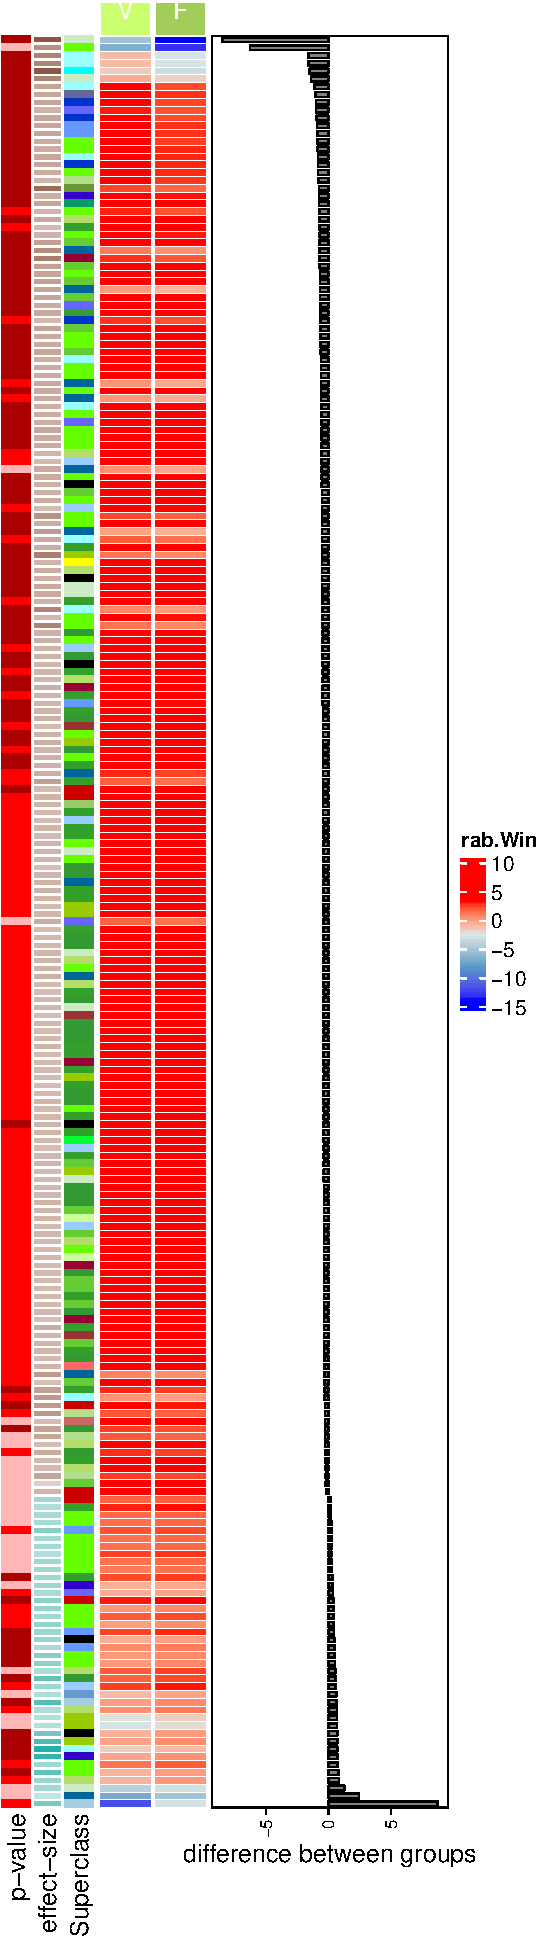
\includegraphics{Doc_pdf_files/figure-latex/unnamed-chunk-43-1} \end{center}

\begin{Shaded}
\begin{Highlighting}[]
\CommentTok{\#pdf("fig\_picrust\_VvsF.pdf", width=7, height=20)}
\CommentTok{\#print(htVvsF)}
\CommentTok{\#dev.off()}
\end{Highlighting}
\end{Shaded}

\hypertarget{vegetative-vs-grainfilling}{%
\paragraph{Vegetative vs
Grainfilling}\label{vegetative-vs-grainfilling}}

\begin{Shaded}
\begin{Highlighting}[]
\CommentTok{\# VvsF}
\NormalTok{aldex\_all\_dif}\OtherTok{\textless{}{-}} \FunctionTok{read\_tsv}\NormalTok{( }\StringTok{"../Data/aldex\_Stage\_vvsg\_picrust.tsv"}\NormalTok{)}


\CommentTok{\#construc heatmap}
\NormalTok{annotation\_heatmap}\OtherTok{\textless{}{-}}\NormalTok{ aldex\_all\_dif}\SpecialCharTok{\%\textgreater{}\%} \FunctionTok{left\_join}\NormalTok{(}
\NormalTok{  levels, }\AttributeTok{by =} \FunctionTok{c}\NormalTok{(}\StringTok{"Feature.ID"}\OtherTok{=}\StringTok{"pathway"}\NormalTok{))}\SpecialCharTok{\%\textgreater{}\%}\NormalTok{ dplyr}\SpecialCharTok{::}\FunctionTok{select}\NormalTok{(}
\NormalTok{  level2, Feature.ID, p.Value, effect, diff.btw) }\SpecialCharTok{\%\textgreater{}\%} \FunctionTok{mutate\_at}\NormalTok{(}
    \FunctionTok{c}\NormalTok{(}\DecValTok{3}\NormalTok{), }\FunctionTok{funs}\NormalTok{(}\AttributeTok{p.value =} \FunctionTok{case\_when}\NormalTok{(}
\NormalTok{    . }\SpecialCharTok{\textless{}=} \FloatTok{0.001} \SpecialCharTok{\textasciitilde{}} \StringTok{"\textless{}0.001"}\NormalTok{,}
\NormalTok{    . }\SpecialCharTok{\textgreater{}}  \FloatTok{0.001} \SpecialCharTok{\&}\NormalTok{ .  }\SpecialCharTok{\textless{}=} \FloatTok{0.01} \SpecialCharTok{\textasciitilde{}} \StringTok{"\textless{}0.01"}\NormalTok{,}
\NormalTok{    . }\SpecialCharTok{\textgreater{}}  \FloatTok{0.01} \SpecialCharTok{\&}\NormalTok{ .  }\SpecialCharTok{\textless{}=} \FloatTok{0.05} \SpecialCharTok{\textasciitilde{}} \StringTok{"\textless{}0.05"}\NormalTok{)))}\SpecialCharTok{\%\textgreater{}\%}\FunctionTok{arrange}\NormalTok{(}
\NormalTok{      diff.btw)}\SpecialCharTok{\%\textgreater{}\%}\FunctionTok{column\_to\_rownames}\NormalTok{(}\AttributeTok{var =} \StringTok{"Feature.ID"}\NormalTok{)}

\NormalTok{data\_heatmap}\OtherTok{\textless{}{-}}\NormalTok{ aldex\_all\_dif }\SpecialCharTok{\%\textgreater{}\%} \FunctionTok{arrange}\NormalTok{(}
\NormalTok{  diff.btw)}\SpecialCharTok{\%\textgreater{}\%}\FunctionTok{column\_to\_rownames}\NormalTok{(}
  \AttributeTok{var =} \StringTok{"Feature.ID"}\NormalTok{)}\SpecialCharTok{\%\textgreater{}\%}\NormalTok{dplyr}\SpecialCharTok{::}\FunctionTok{select}\NormalTok{(}
\NormalTok{    rab.win}\FloatTok{.0}\NormalTok{, rab.win}\FloatTok{.1}\NormalTok{) }\SpecialCharTok{\%\textgreater{}\%}  \FunctionTok{rename}\NormalTok{(}
  \AttributeTok{Ve=}\NormalTok{ rab.win}\FloatTok{.0}\NormalTok{, }\AttributeTok{Gr=}\NormalTok{ rab.win}\FloatTok{.1}\NormalTok{)}

\NormalTok{colAnn }\OtherTok{\textless{}{-}} \FunctionTok{HeatmapAnnotation}\NormalTok{(}
  \AttributeTok{Superclass =}\NormalTok{ annotation\_heatmap}\SpecialCharTok{$}\NormalTok{level2,}
  \AttributeTok{which =} \StringTok{\textquotesingle{}row\textquotesingle{}}\NormalTok{,}
  \AttributeTok{col =}\NormalTok{ cols\_ann,}
  \AttributeTok{show\_legend =}\NormalTok{ F)}

\NormalTok{cols\_pvalue }\OtherTok{\textless{}{-}} \FunctionTok{list}\NormalTok{(}
  \StringTok{\textquotesingle{}p{-}value\textquotesingle{}} \OtherTok{=} \FunctionTok{c}\NormalTok{(}\StringTok{"\textless{}0.001"} \OtherTok{=} \StringTok{\textquotesingle{}\#AB0000\textquotesingle{}}\NormalTok{,}
  \StringTok{"\textless{}0.01"} \OtherTok{=} \StringTok{\textquotesingle{}\#FF0000\textquotesingle{}}\NormalTok{,}
  \StringTok{"\textless{}0.05"}\OtherTok{=}\StringTok{"\#FFB6B6"}\NormalTok{))}

\NormalTok{annP2 }\OtherTok{=} \FunctionTok{HeatmapAnnotation}\NormalTok{(}
  \StringTok{"p{-}value"} \OtherTok{=}\NormalTok{ annotation\_heatmap}\SpecialCharTok{$}\NormalTok{p.value,}
   \AttributeTok{which =} \StringTok{"row"}\NormalTok{, }\AttributeTok{col =}\NormalTok{ cols\_pvalue,}
   \AttributeTok{show\_legend =}\NormalTok{ F)}


\CommentTok{\#effect annotation}
\NormalTok{annEffect }\OtherTok{=} \FunctionTok{HeatmapAnnotation}\NormalTok{(}
  \StringTok{"effect{-}size"} \OtherTok{=}\NormalTok{ annotation\_heatmap}\SpecialCharTok{$}\NormalTok{effect,}
  \AttributeTok{which =} \StringTok{"row"}\NormalTok{, }\AttributeTok{col =} \FunctionTok{list}\NormalTok{(}
  \StringTok{"effect{-}size"} \OtherTok{=}\NormalTok{ effect\_col\_fun),}
  \AttributeTok{show\_legend  =}\NormalTok{F, }
  \AttributeTok{gp =} \FunctionTok{gpar}\NormalTok{(}\AttributeTok{col =} \StringTok{"white"}\NormalTok{))}

\NormalTok{bardif}\OtherTok{=} \FunctionTok{rowAnnotation}\NormalTok{(}
  \StringTok{"difference between groups"} \OtherTok{=} \FunctionTok{anno\_barplot}\NormalTok{(}
\NormalTok{    annotation\_heatmap}\SpecialCharTok{$}\NormalTok{diff.btw, }\AttributeTok{width =} \FunctionTok{unit}\NormalTok{(}\DecValTok{4}\NormalTok{, }\StringTok{"cm"}\NormalTok{)))}



\NormalTok{htVvsG}\OtherTok{\textless{}{-}}\NormalTok{ComplexHeatmap}\SpecialCharTok{::}\FunctionTok{Heatmap}\NormalTok{(}
\NormalTok{  data\_heatmap, }\AttributeTok{col =}\NormalTok{ color\_heatmap, }\AttributeTok{row\_dend\_reorder =}\NormalTok{ F, }
  \AttributeTok{width =} \FunctionTok{ncol}\NormalTok{(data\_heatmap)}\SpecialCharTok{*}\FunctionTok{unit}\NormalTok{(}\FloatTok{0.9}\NormalTok{, }\StringTok{"cm"}\NormalTok{),}
  \AttributeTok{height =} \FunctionTok{ncol}\NormalTok{(data\_heatmap)}\SpecialCharTok{*}\FunctionTok{unit}\NormalTok{(}\DecValTok{14}\NormalTok{, }\StringTok{"cm"}\NormalTok{),}
  \AttributeTok{left\_annotation =}  \FunctionTok{c}\NormalTok{(annP2, annEffect, colAnn),}
  \AttributeTok{heatmap\_legend\_param =} \FunctionTok{list}\NormalTok{(}\AttributeTok{direction =} \StringTok{"vertical"}\NormalTok{ ),}
  \AttributeTok{right\_annotation =} \FunctionTok{c}\NormalTok{(bardif),}
  \AttributeTok{cluster\_column\_slices =} \ConstantTok{FALSE}\NormalTok{,}
  \AttributeTok{column\_split =} \FunctionTok{factor}\NormalTok{(}\FunctionTok{rep}\NormalTok{(}\FunctionTok{c}\NormalTok{(}\StringTok{"V"}\NormalTok{, }\StringTok{"G"}\NormalTok{)), }\AttributeTok{levels =} \FunctionTok{c}\NormalTok{(}\StringTok{"V"}\NormalTok{, }\StringTok{"G"}\NormalTok{)),}
  \AttributeTok{cluster\_rows =}\NormalTok{ F,}\AttributeTok{show\_heatmap\_legend =}\NormalTok{ T,}
  \AttributeTok{column\_km =} \DecValTok{1}\NormalTok{, }\AttributeTok{column\_title\_gp =} \FunctionTok{gpar}\NormalTok{(}\AttributeTok{fill =} \FunctionTok{c}\NormalTok{(}
  \StringTok{"darkolivegreen1"}\NormalTok{,}\StringTok{"darkolivegreen"}\NormalTok{), }\AttributeTok{col=}\StringTok{"white"}\NormalTok{),}
  \AttributeTok{border =}\NormalTok{ F, }\AttributeTok{column\_gap =} \FunctionTok{unit}\NormalTok{(}\FloatTok{0.5}\NormalTok{, }\StringTok{"mm"}\NormalTok{), }
  \AttributeTok{row\_dend\_side =} \StringTok{"left"}\NormalTok{,}\AttributeTok{row\_names\_side =} \StringTok{"right"}\NormalTok{,}\AttributeTok{show\_row\_names =}\NormalTok{ F ,}
  \AttributeTok{rect\_gp =} \FunctionTok{gpar}\NormalTok{(}\AttributeTok{col =} \StringTok{"white"}\NormalTok{, }\AttributeTok{lwd =} \FloatTok{0.2}\NormalTok{), }
  \AttributeTok{row\_names\_gp =} \FunctionTok{gpar}\NormalTok{(}\AttributeTok{fontface =}\StringTok{"italic"}\NormalTok{, }\AttributeTok{fontsize=}\DecValTok{10}\NormalTok{),}
  \AttributeTok{cluster\_columns =}\NormalTok{ F,}
  \AttributeTok{show\_column\_names =}\NormalTok{ F, }\AttributeTok{name =} \StringTok{"rab.Win"}\NormalTok{)}


\NormalTok{htVvsG   }
\end{Highlighting}
\end{Shaded}

\begin{center}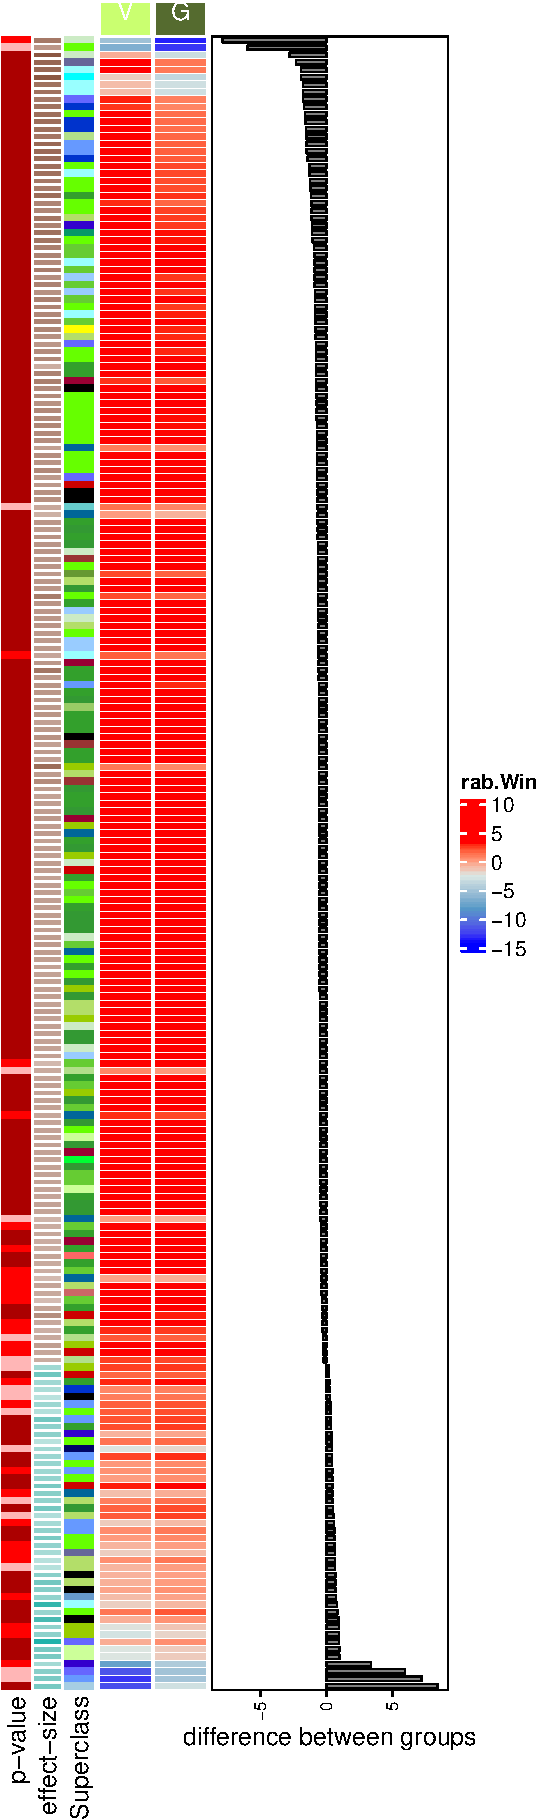
\includegraphics{Doc_pdf_files/figure-latex/unnamed-chunk-44-1} \end{center}

\begin{Shaded}
\begin{Highlighting}[]
\CommentTok{\#pdf("fig\_picrust\_VvsG.pdf", width=7, height=20)}
\CommentTok{\#print(htVvsG)}
\CommentTok{\#dev.off()}
\end{Highlighting}
\end{Shaded}

\hypertarget{flowering-vs-grainfilling}{%
\paragraph{Flowering vs Grainfilling}\label{flowering-vs-grainfilling}}

\begin{Shaded}
\begin{Highlighting}[]
\NormalTok{aldex\_all\_dif}\OtherTok{\textless{}{-}} \FunctionTok{read\_tsv}\NormalTok{( }\StringTok{"../Data/aldex\_Stage\_fvsg\_picrust.tsv"}\NormalTok{)}


\CommentTok{\#construc heatmap}
\NormalTok{annotation\_heatmap}\OtherTok{\textless{}{-}}\NormalTok{ aldex\_all\_dif}\SpecialCharTok{\%\textgreater{}\%} \FunctionTok{left\_join}\NormalTok{(}
\NormalTok{  levels, }\AttributeTok{by =} \FunctionTok{c}\NormalTok{(}\StringTok{"Feature.ID"}\OtherTok{=}\StringTok{"pathway"}\NormalTok{))}\SpecialCharTok{\%\textgreater{}\%}\NormalTok{ dplyr}\SpecialCharTok{::}\FunctionTok{select}\NormalTok{(}
\NormalTok{  level2, Feature.ID, p.Value, effect, diff.btw) }\SpecialCharTok{\%\textgreater{}\%} \FunctionTok{mutate\_at}\NormalTok{(}
  \FunctionTok{c}\NormalTok{(}\DecValTok{3}\NormalTok{), }\FunctionTok{funs}\NormalTok{(}\AttributeTok{p.value =} \FunctionTok{case\_when}\NormalTok{(}
\NormalTok{  . }\SpecialCharTok{\textless{}=} \FloatTok{0.001} \SpecialCharTok{\textasciitilde{}} \StringTok{"\textless{}0.001"}\NormalTok{,}
\NormalTok{  . }\SpecialCharTok{\textgreater{}}  \FloatTok{0.001} \SpecialCharTok{\&}\NormalTok{ .  }\SpecialCharTok{\textless{}=} \FloatTok{0.01} \SpecialCharTok{\textasciitilde{}} \StringTok{"\textless{}0.01"}\NormalTok{,}
\NormalTok{  . }\SpecialCharTok{\textgreater{}}  \FloatTok{0.01} \SpecialCharTok{\&}\NormalTok{ .  }\SpecialCharTok{\textless{}=} \FloatTok{0.05} \SpecialCharTok{\textasciitilde{}} \StringTok{"\textless{}0.05"}\NormalTok{)))}\SpecialCharTok{\%\textgreater{}\%}\FunctionTok{arrange}\NormalTok{(}
\NormalTok{  diff.btw)}\SpecialCharTok{\%\textgreater{}\%}\FunctionTok{column\_to\_rownames}\NormalTok{(}\AttributeTok{var =} \StringTok{"Feature.ID"}\NormalTok{)}

\NormalTok{data\_heatmap}\OtherTok{\textless{}{-}}\NormalTok{ aldex\_all\_dif }\SpecialCharTok{\%\textgreater{}\%} \FunctionTok{arrange}\NormalTok{(}
\NormalTok{  diff.btw)}\SpecialCharTok{\%\textgreater{}\%}\FunctionTok{column\_to\_rownames}\NormalTok{(}
  \AttributeTok{var =} \StringTok{"Feature.ID"}\NormalTok{)}\SpecialCharTok{\%\textgreater{}\%}\NormalTok{dplyr}\SpecialCharTok{::}\FunctionTok{select}\NormalTok{(}
\NormalTok{  rab.win}\FloatTok{.0}\NormalTok{, rab.win}\FloatTok{.1}\NormalTok{) }\SpecialCharTok{\%\textgreater{}\%} \FunctionTok{rename}\NormalTok{(}
  \AttributeTok{Fl =}\NormalTok{ rab.win}\FloatTok{.0}\NormalTok{, }\AttributeTok{Gr=}\NormalTok{ rab.win}\FloatTok{.1}\NormalTok{)}

\NormalTok{colAnn }\OtherTok{\textless{}{-}} \FunctionTok{HeatmapAnnotation}\NormalTok{(}
  \AttributeTok{Superclass =}\NormalTok{ annotation\_heatmap}\SpecialCharTok{$}\NormalTok{level2,}
  \AttributeTok{which =} \StringTok{\textquotesingle{}row\textquotesingle{}}\NormalTok{,}
  \AttributeTok{col =}\NormalTok{ cols\_ann,}
  \AttributeTok{show\_legend =}\NormalTok{ F)}

\NormalTok{cols\_pvalue }\OtherTok{\textless{}{-}} \FunctionTok{list}\NormalTok{(}
  \StringTok{\textquotesingle{}p{-}value\textquotesingle{}} \OtherTok{=} \FunctionTok{c}\NormalTok{(}\StringTok{"\textless{}0.001"} \OtherTok{=} \StringTok{\textquotesingle{}\#AB0000\textquotesingle{}}\NormalTok{,}
  \StringTok{"\textless{}0.01"} \OtherTok{=} \StringTok{\textquotesingle{}\#FF0000\textquotesingle{}}\NormalTok{,}
  \StringTok{"\textless{}0.05"}\OtherTok{=}\StringTok{"\#FFB6B6"}\NormalTok{))}

\NormalTok{annP2 }\OtherTok{=} \FunctionTok{HeatmapAnnotation}\NormalTok{(}
  \StringTok{"p{-}value"} \OtherTok{=}\NormalTok{ annotation\_heatmap}\SpecialCharTok{$}\NormalTok{p.value,}
   \AttributeTok{which =} \StringTok{"row"}\NormalTok{, }\AttributeTok{col =}\NormalTok{ cols\_pvalue,}
   \AttributeTok{show\_legend =}\NormalTok{ F)}

\CommentTok{\#effect annotation}

\NormalTok{annEffect }\OtherTok{=} \FunctionTok{HeatmapAnnotation}\NormalTok{(}
  \StringTok{"effect{-}size"} \OtherTok{=}\NormalTok{ annotation\_heatmap}\SpecialCharTok{$}\NormalTok{effect,}
   \AttributeTok{which =} \StringTok{"row"}\NormalTok{, }\AttributeTok{col =} \FunctionTok{list}\NormalTok{(}\StringTok{"effect{-}size"} \OtherTok{=}\NormalTok{ effect\_col\_fun),}
   \AttributeTok{show\_legend  =}\NormalTok{F, }
   \AttributeTok{gp =} \FunctionTok{gpar}\NormalTok{(}\AttributeTok{col =} \StringTok{"white"}\NormalTok{))}

\NormalTok{bardif}\OtherTok{=} \FunctionTok{rowAnnotation}\NormalTok{(}
  \StringTok{"difference between groups"} \OtherTok{=} \FunctionTok{anno\_barplot}\NormalTok{(}
\NormalTok{    annotation\_heatmap}\SpecialCharTok{$}\NormalTok{diff.btw, }\AttributeTok{width =} \FunctionTok{unit}\NormalTok{(}\DecValTok{4}\NormalTok{, }\StringTok{"cm"}\NormalTok{)))}



\NormalTok{htFvsG}\OtherTok{\textless{}{-}}\NormalTok{ComplexHeatmap}\SpecialCharTok{::}\FunctionTok{Heatmap}\NormalTok{(}
\NormalTok{  data\_heatmap, }\AttributeTok{col =}\NormalTok{ color\_heatmap, }\AttributeTok{row\_dend\_reorder =}\NormalTok{ F, }
  \AttributeTok{width =} \FunctionTok{ncol}\NormalTok{(data\_heatmap)}\SpecialCharTok{*}\FunctionTok{unit}\NormalTok{(}\FloatTok{0.9}\NormalTok{, }\StringTok{"cm"}\NormalTok{),}
  \AttributeTok{height =} \FunctionTok{ncol}\NormalTok{(data\_heatmap)}\SpecialCharTok{*}\FunctionTok{unit}\NormalTok{(}\DecValTok{7}\NormalTok{, }\StringTok{"cm"}\NormalTok{),}
  \AttributeTok{left\_annotation =}  \FunctionTok{c}\NormalTok{(annP2, annEffect, colAnn),}
  \AttributeTok{heatmap\_legend\_param =} \FunctionTok{list}\NormalTok{(}\AttributeTok{direction =} \StringTok{"vertical"}\NormalTok{ ),}
  \AttributeTok{right\_annotation =} \FunctionTok{c}\NormalTok{(bardif),}
  \AttributeTok{column\_split =} \FunctionTok{rep}\NormalTok{(}\FunctionTok{c}\NormalTok{(}\StringTok{"F"}\NormalTok{, }\StringTok{"G"}\NormalTok{)),}
  \AttributeTok{cluster\_rows =}\NormalTok{ F, }\AttributeTok{show\_heatmap\_legend =}\NormalTok{ T,}
  \AttributeTok{cluster\_column\_slices =}\NormalTok{ F,}
  \AttributeTok{column\_km =} \DecValTok{1}\NormalTok{, }\AttributeTok{column\_title\_gp =} \FunctionTok{gpar}\NormalTok{(}
  \AttributeTok{fill =} \FunctionTok{c}\NormalTok{(}\StringTok{"darkolivegreen3"}\NormalTok{,}\StringTok{"darkolivegreen"}\NormalTok{ ), }\AttributeTok{col=}\StringTok{"white"}\NormalTok{),}
  \AttributeTok{border =}\NormalTok{ F, }\AttributeTok{column\_gap =} \FunctionTok{unit}\NormalTok{(}\FloatTok{0.5}\NormalTok{, }\StringTok{"mm"}\NormalTok{),}
  \AttributeTok{cluster\_columns =}\NormalTok{ F,}
  \AttributeTok{row\_dend\_side =} \StringTok{"left"}\NormalTok{,}\AttributeTok{row\_names\_side =} \StringTok{"right"}\NormalTok{,}\AttributeTok{show\_row\_names =}\NormalTok{ F ,}
  \AttributeTok{rect\_gp =} \FunctionTok{gpar}\NormalTok{(}\AttributeTok{col =} \StringTok{"white"}\NormalTok{, }\AttributeTok{lwd =} \FloatTok{0.2}\NormalTok{), }\AttributeTok{row\_names\_gp =} \FunctionTok{gpar}\NormalTok{(}
  \AttributeTok{fontface =}\StringTok{"italic"}\NormalTok{, }\AttributeTok{fontsize=}\DecValTok{10}\NormalTok{),}\AttributeTok{show\_column\_names =}\NormalTok{ F, }\AttributeTok{name =} \StringTok{"rab.Win"}\NormalTok{)}

\NormalTok{htFvsG}
\end{Highlighting}
\end{Shaded}

\begin{center}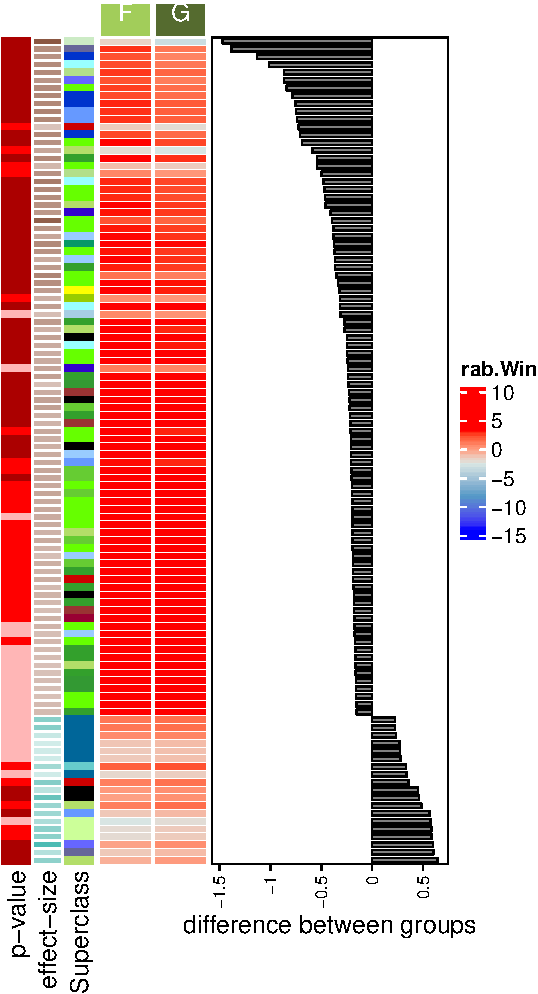
\includegraphics{Doc_pdf_files/figure-latex/unnamed-chunk-45-1} \end{center}

\begin{Shaded}
\begin{Highlighting}[]
\CommentTok{\#pdf("fig\_picrust\_FvsG.pdf", width=7, height=20)}
\CommentTok{\#print(htFvsG)}
\CommentTok{\#dev.off()}
\end{Highlighting}
\end{Shaded}

\hypertarget{viii.-picrust2-plot}{%
\section{VIII. PICRUST2 PLOT}\label{viii.-picrust2-plot}}

\hypertarget{loading-libraries-6}{%
\subsubsection{Loading libraries}\label{loading-libraries-6}}

\begin{Shaded}
\begin{Highlighting}[]
\FunctionTok{library}\NormalTok{(ComplexHeatmap)}
\FunctionTok{library}\NormalTok{(tidyverse)}
\FunctionTok{library}\NormalTok{(circlize)}
\FunctionTok{library}\NormalTok{(viridis)}
\FunctionTok{library}\NormalTok{(RColorBrewer)}
\FunctionTok{library}\NormalTok{(cowplot)}
\end{Highlighting}
\end{Shaded}

\hypertarget{loadings-files}{%
\subsubsection{Loadings files}\label{loadings-files}}

\begin{Shaded}
\begin{Highlighting}[]
\NormalTok{aldex\_all\_dif\_soil}\OtherTok{\textless{}{-}} \FunctionTok{read\_tsv}\NormalTok{( }\StringTok{"../Data/aldex\_Soil\_picrust.tsv"}\NormalTok{) }\SpecialCharTok{\%\textgreater{}\%} \FunctionTok{arrange}\NormalTok{(diff.btw)}
\NormalTok{aldex\_all\_dif\_Treatment}\OtherTok{\textless{}{-}} \FunctionTok{read\_tsv}\NormalTok{( }\StringTok{"../Data/aldex\_Treatment\_picrust.tsv"}\NormalTok{)}\SpecialCharTok{\%\textgreater{}\%} \FunctionTok{arrange}\NormalTok{(diff.btw)}
\NormalTok{aldex\_all\_dif\_Stage\_vvsf}\OtherTok{\textless{}{-}} \FunctionTok{read\_tsv}\NormalTok{( }\StringTok{"../Data/aldex\_Stage\_vvsf\_picrust.tsv"}\NormalTok{)}\SpecialCharTok{\%\textgreater{}\%} \FunctionTok{arrange}\NormalTok{(diff.btw)}
\NormalTok{aldex\_all\_dif\_Stage\_vvsg}\OtherTok{\textless{}{-}} \FunctionTok{read\_tsv}\NormalTok{( }\StringTok{"../Data/aldex\_Stage\_vvsg\_picrust.tsv"}\NormalTok{)}\SpecialCharTok{\%\textgreater{}\%} \FunctionTok{arrange}\NormalTok{(diff.btw)}
\NormalTok{aldex\_all\_dif\_Stage\_fvsg}\OtherTok{\textless{}{-}} \FunctionTok{read\_tsv}\NormalTok{( }\StringTok{"../Data/aldex\_Stage\_fvsg\_picrust.tsv"}\NormalTok{)}\SpecialCharTok{\%\textgreater{}\%} \FunctionTok{arrange}\NormalTok{(diff.btw)}
\end{Highlighting}
\end{Shaded}

\hypertarget{formatting-files}{%
\subsubsection{Formatting files}\label{formatting-files}}

\begin{Shaded}
\begin{Highlighting}[]
\NormalTok{a}\OtherTok{\textless{}{-}}\NormalTok{aldex\_all\_dif\_soil }\SpecialCharTok{\%\textgreater{}\%}  \FunctionTok{mutate}\NormalTok{(}\AttributeTok{Dif =} \FunctionTok{case\_when}\NormalTok{(}
\NormalTok{  diff.btw }\SpecialCharTok{\textless{}} \DecValTok{0} \SpecialCharTok{\textasciitilde{}} \StringTok{"RH"}\NormalTok{,}
\NormalTok{  diff.btw }\SpecialCharTok{\textgreater{}} \DecValTok{0}  \SpecialCharTok{\textasciitilde{}} \StringTok{"BS"}\NormalTok{)) }\SpecialCharTok{\%\textgreater{}\%} \FunctionTok{group\_by}\NormalTok{(Dif) }\SpecialCharTok{\%\textgreater{}\%}
  \FunctionTok{summarise}\NormalTok{(}\AttributeTok{n =} \FunctionTok{n}\NormalTok{()) }\SpecialCharTok{\%\textgreater{}\%} 
  \FunctionTok{mutate}\NormalTok{(}\AttributeTok{freq =} \FunctionTok{round}\NormalTok{(n }\SpecialCharTok{/} \FunctionTok{sum}\NormalTok{(n)}\SpecialCharTok{*}\DecValTok{100}\NormalTok{)) }\SpecialCharTok{\%\textgreater{}\%} \FunctionTok{mutate}\NormalTok{(}\AttributeTok{type =} \StringTok{"BS vs Rh }\SpecialCharTok{\textbackslash{}n}\StringTok{  Soil"}\NormalTok{)}

\NormalTok{b}\OtherTok{\textless{}{-}}\NormalTok{aldex\_all\_dif\_Treatment }\SpecialCharTok{\%\textgreater{}\%}  \FunctionTok{mutate}\NormalTok{(}\AttributeTok{Dif =} \FunctionTok{case\_when}\NormalTok{(}
\NormalTok{  diff.btw }\SpecialCharTok{\textless{}} \DecValTok{0} \SpecialCharTok{\textasciitilde{}} \StringTok{"CA"}\NormalTok{,}
\NormalTok{  diff.btw }\SpecialCharTok{\textgreater{}} \DecValTok{0}  \SpecialCharTok{\textasciitilde{}} \StringTok{"CP"}\NormalTok{)) }\SpecialCharTok{\%\textgreater{}\%} \FunctionTok{group\_by}\NormalTok{(Dif) }\SpecialCharTok{\%\textgreater{}\%}
  \FunctionTok{summarise}\NormalTok{(}\AttributeTok{n =} \FunctionTok{n}\NormalTok{()) }\SpecialCharTok{\%\textgreater{}\%}
  \FunctionTok{mutate}\NormalTok{(}\AttributeTok{freq =} \FunctionTok{round}\NormalTok{(n }\SpecialCharTok{/} \FunctionTok{sum}\NormalTok{(n)}\SpecialCharTok{*}\DecValTok{100}\NormalTok{))}\SpecialCharTok{\%\textgreater{}\%} \FunctionTok{mutate}\NormalTok{(}\AttributeTok{type =} \StringTok{"CA vs CP }\SpecialCharTok{\textbackslash{}n}\StringTok{ Practice"}\NormalTok{)}

\NormalTok{c}\OtherTok{\textless{}{-}}\NormalTok{aldex\_all\_dif\_Stage\_vvsf }\SpecialCharTok{\%\textgreater{}\%}  \FunctionTok{mutate}\NormalTok{(}\AttributeTok{Dif =} \FunctionTok{case\_when}\NormalTok{(}
\NormalTok{  diff.btw }\SpecialCharTok{\textless{}} \DecValTok{0} \SpecialCharTok{\textasciitilde{}} \StringTok{"V"}\NormalTok{,}
\NormalTok{  diff.btw }\SpecialCharTok{\textgreater{}} \DecValTok{0}  \SpecialCharTok{\textasciitilde{}} \StringTok{"F"}\NormalTok{)) }\SpecialCharTok{\%\textgreater{}\%} \FunctionTok{group\_by}\NormalTok{(Dif) }\SpecialCharTok{\%\textgreater{}\%}
  \FunctionTok{summarise}\NormalTok{(}\AttributeTok{n =} \FunctionTok{n}\NormalTok{()) }\SpecialCharTok{\%\textgreater{}\%}
  \FunctionTok{mutate}\NormalTok{(}\AttributeTok{freq =} \FunctionTok{round}\NormalTok{(n }\SpecialCharTok{/} \FunctionTok{sum}\NormalTok{(n)}\SpecialCharTok{*}\DecValTok{100}\NormalTok{))}\SpecialCharTok{\%\textgreater{}\%} \FunctionTok{mutate}\NormalTok{(}\AttributeTok{type =} \StringTok{"V vs F }\SpecialCharTok{\textbackslash{}n}\StringTok{  Stage"}\NormalTok{)}

\NormalTok{d}\OtherTok{\textless{}{-}}\NormalTok{aldex\_all\_dif\_Stage\_vvsg }\SpecialCharTok{\%\textgreater{}\%}  \FunctionTok{mutate}\NormalTok{(}\AttributeTok{Dif =} \FunctionTok{case\_when}\NormalTok{(}
\NormalTok{  diff.btw }\SpecialCharTok{\textless{}} \DecValTok{0} \SpecialCharTok{\textasciitilde{}} \StringTok{"V"}\NormalTok{,}
\NormalTok{  diff.btw }\SpecialCharTok{\textgreater{}} \DecValTok{0}  \SpecialCharTok{\textasciitilde{}} \StringTok{"G"}\NormalTok{)) }\SpecialCharTok{\%\textgreater{}\%} \FunctionTok{group\_by}\NormalTok{(Dif) }\SpecialCharTok{\%\textgreater{}\%}
  \FunctionTok{summarise}\NormalTok{(}\AttributeTok{n =} \FunctionTok{n}\NormalTok{()) }\SpecialCharTok{\%\textgreater{}\%}
  \FunctionTok{mutate}\NormalTok{(}\AttributeTok{freq =} \FunctionTok{round}\NormalTok{(n }\SpecialCharTok{/} \FunctionTok{sum}\NormalTok{(n)}\SpecialCharTok{*}\DecValTok{100}\NormalTok{))}\SpecialCharTok{\%\textgreater{}\%} \FunctionTok{mutate}\NormalTok{(}\AttributeTok{type =} \StringTok{"V vs G }\SpecialCharTok{\textbackslash{}n}\StringTok{  Stage"}\NormalTok{)}

\NormalTok{e}\OtherTok{\textless{}{-}}\NormalTok{aldex\_all\_dif\_Stage\_fvsg}\SpecialCharTok{\%\textgreater{}\%}  \FunctionTok{mutate}\NormalTok{(}\AttributeTok{Dif =} \FunctionTok{case\_when}\NormalTok{(}
\NormalTok{  diff.btw }\SpecialCharTok{\textless{}} \DecValTok{0} \SpecialCharTok{\textasciitilde{}} \StringTok{"F"}\NormalTok{,}
\NormalTok{  diff.btw }\SpecialCharTok{\textgreater{}} \DecValTok{0}  \SpecialCharTok{\textasciitilde{}} \StringTok{"G"}\NormalTok{)) }\SpecialCharTok{\%\textgreater{}\%} \FunctionTok{group\_by}\NormalTok{(Dif) }\SpecialCharTok{\%\textgreater{}\%}
  \FunctionTok{summarise}\NormalTok{(}\AttributeTok{n =} \FunctionTok{n}\NormalTok{()) }\SpecialCharTok{\%\textgreater{}\%}
  \FunctionTok{mutate}\NormalTok{(}\AttributeTok{freq =} \FunctionTok{round}\NormalTok{(n }\SpecialCharTok{/} \FunctionTok{sum}\NormalTok{(n)}\SpecialCharTok{*}\DecValTok{100}\NormalTok{))}\SpecialCharTok{\%\textgreater{}\%} \FunctionTok{mutate}\NormalTok{(}\AttributeTok{type =} \StringTok{"F vs G }\SpecialCharTok{\textbackslash{}n}\StringTok{ Stage"}\NormalTok{)}

\CommentTok{\#joining all files}
\NormalTok{graph}\OtherTok{\textless{}{-}} \FunctionTok{rbind}\NormalTok{(a,b,c,d,e) }\SpecialCharTok{\%\textgreater{}\%}\FunctionTok{mutate}\NormalTok{(}
  \AttributeTok{freq2=} \FunctionTok{paste}\NormalTok{(freq,}\StringTok{"\%"}\NormalTok{, }\AttributeTok{sep =} \StringTok{""}\NormalTok{))}

\CommentTok{\#setting labels (sum of n by type)}

\NormalTok{label2}\OtherTok{\textless{}{-}} \FunctionTok{paste}\NormalTok{(}\StringTok{"n="}\NormalTok{,graph}\SpecialCharTok{$}\NormalTok{n[}\DecValTok{1}\NormalTok{]}\SpecialCharTok{+}\NormalTok{graph}\SpecialCharTok{$}\NormalTok{n[}\DecValTok{2}\NormalTok{], }\AttributeTok{sep =} \StringTok{""}\NormalTok{)}
\NormalTok{label1}\OtherTok{\textless{}{-}} \FunctionTok{paste}\NormalTok{(}\StringTok{"n="}\NormalTok{,graph}\SpecialCharTok{$}\NormalTok{n[}\DecValTok{3}\NormalTok{]}\SpecialCharTok{+}\NormalTok{graph}\SpecialCharTok{$}\NormalTok{n[}\DecValTok{4}\NormalTok{], }\AttributeTok{sep =} \StringTok{""}\NormalTok{)}
\NormalTok{label5}\OtherTok{\textless{}{-}} \FunctionTok{paste}\NormalTok{(}\StringTok{"n="}\NormalTok{,graph}\SpecialCharTok{$}\NormalTok{n[}\DecValTok{5}\NormalTok{]}\SpecialCharTok{+}\NormalTok{graph}\SpecialCharTok{$}\NormalTok{n[}\DecValTok{6}\NormalTok{], }\AttributeTok{sep =} \StringTok{""}\NormalTok{)}
\NormalTok{label4}\OtherTok{\textless{}{-}} \FunctionTok{paste}\NormalTok{(}\StringTok{"n="}\NormalTok{,graph}\SpecialCharTok{$}\NormalTok{n[}\DecValTok{7}\NormalTok{]}\SpecialCharTok{+}\NormalTok{graph}\SpecialCharTok{$}\NormalTok{n[}\DecValTok{8}\NormalTok{], }\AttributeTok{sep =} \StringTok{""}\NormalTok{)}
\NormalTok{label3}\OtherTok{\textless{}{-}} \FunctionTok{paste}\NormalTok{(}\StringTok{"n="}\NormalTok{,graph}\SpecialCharTok{$}\NormalTok{n[}\DecValTok{9}\NormalTok{]}\SpecialCharTok{+}\NormalTok{graph}\SpecialCharTok{$}\NormalTok{n[}\DecValTok{10}\NormalTok{], }\AttributeTok{sep =} \StringTok{""}\NormalTok{)}


\FunctionTok{head}\NormalTok{(graph)}
\end{Highlighting}
\end{Shaded}

\begin{verbatim}
## # A tibble: 6 x 5
##   Dif       n  freq type                   freq2
##   <chr> <int> <dbl> <chr>                  <chr>
## 1 BS      131    76 "BS vs Rh \n  Soil"    76%  
## 2 RH       41    24 "BS vs Rh \n  Soil"    24%  
## 3 CA       39    21 "CA vs CP \n Practice" 21%  
## 4 CP      148    79 "CA vs CP \n Practice" 79%  
## 5 F        40    18 "V vs F \n  Stage"     18%  
## 6 V       187    82 "V vs F \n  Stage"     82%
\end{verbatim}

\hypertarget{barplot}{%
\subsubsection{Barplot}\label{barplot}}

\begin{Shaded}
\begin{Highlighting}[]
\CommentTok{\#annotation to facets}

\NormalTok{ann\_text}\OtherTok{\textless{}{-}}\FunctionTok{data.frame}\NormalTok{(}\AttributeTok{type=}\FunctionTok{c}\NormalTok{(}\StringTok{"BS vs Rh }\SpecialCharTok{\textbackslash{}n}\StringTok{  Soil"}\NormalTok{, }\StringTok{"CA vs CP }\SpecialCharTok{\textbackslash{}n}\StringTok{ Practice"}\NormalTok{,}
                            \StringTok{"F vs G }\SpecialCharTok{\textbackslash{}n}\StringTok{ Stage"}\NormalTok{,}\StringTok{"V vs F }\SpecialCharTok{\textbackslash{}n}\StringTok{  Stage"}\NormalTok{, }\StringTok{"V vs G }\SpecialCharTok{\textbackslash{}n}\StringTok{  Stage"}\NormalTok{),}
                     \AttributeTok{n=}\FunctionTok{c}\NormalTok{(}\DecValTok{200}\NormalTok{,}\DecValTok{200}\NormalTok{,}\DecValTok{120}\NormalTok{, }\DecValTok{250}\NormalTok{, }\DecValTok{250}\NormalTok{),}
                     \AttributeTok{Dif=}\FunctionTok{c}\NormalTok{(}\StringTok{"BS"}\NormalTok{,}\StringTok{"CA"}\NormalTok{,}\StringTok{"G"}\NormalTok{, }\StringTok{"F"}\NormalTok{, }\StringTok{"V"}\NormalTok{),}
                     \AttributeTok{label=}\FunctionTok{c}\NormalTok{(label2, label1, label3, label5, label4))}
\CommentTok{\#plot}

\NormalTok{graphs2}\OtherTok{=}\NormalTok{graph }\SpecialCharTok{\%\textgreater{}\%}  \FunctionTok{ggplot}\NormalTok{(}\FunctionTok{aes}\NormalTok{(}\AttributeTok{x =}\NormalTok{ type, }\AttributeTok{y =}\NormalTok{ n, }\AttributeTok{fill =}\NormalTok{ Dif))}\SpecialCharTok{+} \FunctionTok{geom\_bar}\NormalTok{(}\AttributeTok{stat =} \StringTok{"identity"}\NormalTok{,}\AttributeTok{color=}\StringTok{"black"}\NormalTok{)}\SpecialCharTok{+}\FunctionTok{facet\_wrap}\NormalTok{(}\FunctionTok{vars}\NormalTok{(type), }\AttributeTok{scales =} \StringTok{"free\_x"}\NormalTok{, }\AttributeTok{ncol =} \DecValTok{5}\NormalTok{)}\SpecialCharTok{+}
  \FunctionTok{ylab}\NormalTok{(}\StringTok{"No. of EC number differentially abundant"}\NormalTok{)}\SpecialCharTok{+}
  \FunctionTok{geom\_text}\NormalTok{(}\AttributeTok{data =}\NormalTok{ graph, }\FunctionTok{aes}\NormalTok{(}\AttributeTok{label=}\NormalTok{freq2),}\AttributeTok{position =} \FunctionTok{position\_stack}\NormalTok{(}\AttributeTok{vjust =} \FloatTok{0.5}\NormalTok{),  }\AttributeTok{size=}\DecValTok{4}\NormalTok{, }\AttributeTok{color =} \StringTok{"gold3"}\NormalTok{, }\AttributeTok{fontface=}\StringTok{"bold"}\NormalTok{)}\SpecialCharTok{+}
  \FunctionTok{geom\_text}\NormalTok{(}\AttributeTok{data =}\NormalTok{ ann\_text,}\AttributeTok{label=}\NormalTok{ann\_text}\SpecialCharTok{$}\NormalTok{label)  }\SpecialCharTok{+} \FunctionTok{theme\_bw}\NormalTok{()}\SpecialCharTok{+}
  \FunctionTok{theme}\NormalTok{(}\AttributeTok{panel.spacing=}\FunctionTok{unit}\NormalTok{(}\DecValTok{1}\NormalTok{,}\StringTok{"lines"}\NormalTok{), }
        \AttributeTok{strip.text.x =} \FunctionTok{element\_text}\NormalTok{(}\AttributeTok{size =} \DecValTok{12}\NormalTok{),}
        \AttributeTok{axis.text.y =}  \FunctionTok{element\_text}\NormalTok{(}\AttributeTok{colour =} \StringTok{"black"}\NormalTok{, }\AttributeTok{size =} \DecValTok{14}\NormalTok{),}
        \AttributeTok{axis.text.x =} \FunctionTok{element\_blank}\NormalTok{(),}
        \AttributeTok{axis.title.x =} \FunctionTok{element\_blank}\NormalTok{(), }
        \AttributeTok{axis.ticks.x=}\FunctionTok{element\_blank}\NormalTok{(), }
        \AttributeTok{axis.title.y =} \FunctionTok{element\_text}\NormalTok{(}\AttributeTok{size =} \DecValTok{14}\NormalTok{), }
        \AttributeTok{legend.title =} \FunctionTok{element\_text}\NormalTok{(}\AttributeTok{size =} \DecValTok{12}\NormalTok{),}
        \AttributeTok{legend.text =} \FunctionTok{element\_text}\NormalTok{(}\AttributeTok{size=}\DecValTok{12}\NormalTok{), }
        \AttributeTok{panel.grid.major =} \FunctionTok{element\_blank}\NormalTok{(), }\AttributeTok{panel.grid.minor =} \FunctionTok{element\_blank}\NormalTok{(),}
        \AttributeTok{legend.direction =} \StringTok{"vertical"}\NormalTok{ ,}
        \AttributeTok{legend.position =} \StringTok{"none"}\NormalTok{)}\SpecialCharTok{+}\FunctionTok{scale\_fill\_manual}\NormalTok{(}
          \AttributeTok{values =} \FunctionTok{c}\NormalTok{(}\StringTok{"darkgoldenrod4"}\NormalTok{,}
                     \StringTok{"\#212F3D"}\NormalTok{, }\StringTok{"\#839192"}\NormalTok{,}\StringTok{"darkolivegreen3"}\NormalTok{,}
                     \StringTok{"darkolivegreen"}\NormalTok{,}
                     \StringTok{"\#365238"}\NormalTok{, }\StringTok{"darkolivegreen1"}\NormalTok{))}
\NormalTok{   graphs2}
\end{Highlighting}
\end{Shaded}

\begin{center}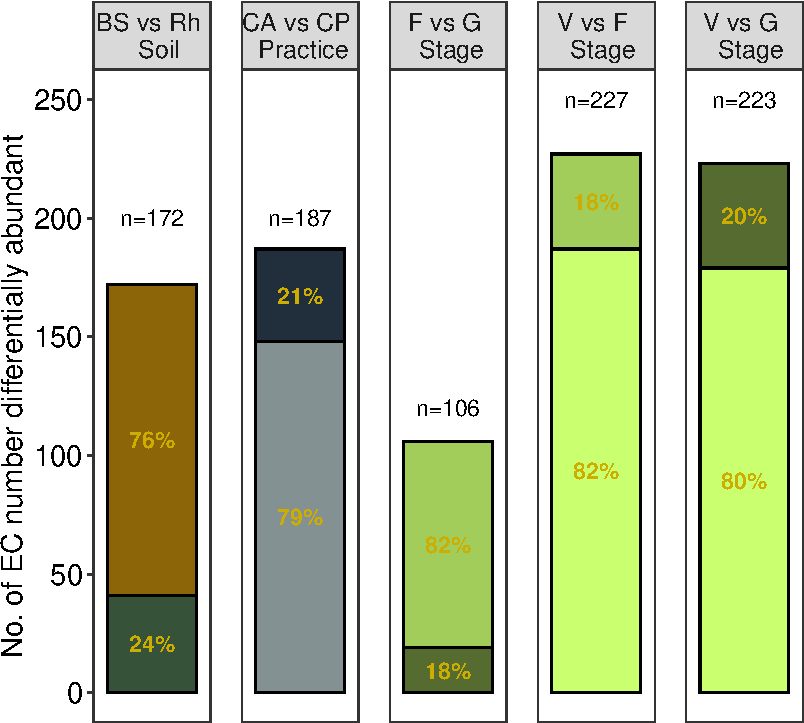
\includegraphics{Doc_pdf_files/figure-latex/unnamed-chunk-49-1} \end{center}

\begin{Shaded}
\begin{Highlighting}[]
\CommentTok{\#pdf("fig\_picrust\_ECnumber.pdf", width=5.5, height=5)}
\CommentTok{\#print(graphs2)}
\CommentTok{\#dev.off()}
\end{Highlighting}
\end{Shaded}


\bibliographystyle{tfcad}
\bibliography{references.bib}




\end{document}
